%&preformat-disser
\RequirePackage[l2tabu,orthodox]{nag} % Раскомментировав, можно в логе получать рекомендации относительно правильного использования пакетов и предупреждения об устаревших и нерекомендуемых пакетах
% Формат А4, 14pt (ГОСТ Р 7.0.11-2011, 5.3.6)
\documentclass[a4paper,14pt,oneside,openany]{memoir}

\input{common/setup}            % общие настройки шаблона
\input{common/packages}         % Пакеты общие для диссертации и автореферата
\synopsisfalse                      % Этот документ --- не автореферат
\input{Dissertation/dispackages}    % Пакеты для диссертации
\input{Dissertation/userpackages}   % Пакеты для специфических пользовательских задач

\input{Dissertation/setup}      % Упрощённые настройки шаблона

\input{common/newnames}         % Новые переменные, для всего проекта

%%% Основные сведения %%%
\newcommand{\thesisAuthorLastName}{Хилькевич}
\newcommand{\thesisAuthorOtherNames}{Евгений Михайлович}
\newcommand{\thesisAuthorInitials}{Е.\,М.}
\newcommand{\thesisAuthor}             % Диссертация, ФИО автора
{%
    \texorpdfstring{% \texorpdfstring takes two arguments and uses the first for (La)TeX and the second for pdf
        \thesisAuthorLastName~\thesisAuthorOtherNames% так будет отображаться на титульном листе или в тексте, где будет использоваться переменная
    }{%
        \thesisAuthorLastName, \thesisAuthorOtherNames% эта запись для свойств pdf-файла. В таком виде, если pdf будет обработан программами для сбора библиографических сведений, будет правильно представлена фамилия.
    }
}
\newcommand{\thesisAuthorShort}        % Диссертация, ФИО автора инициалами
{\thesisAuthorInitials~\thesisAuthorLastName}
%\newcommand{\thesisUdk}                % Диссертация, УДК
%{\fixme{xxx.xxx}}
\newcommand{\thesisTitle}              % Диссертация, название
{Восстановление распределений убегающих электронов в~плазме токамаков JET и ASDEX Upgrade
по измеренному жесткому рентгеновскому излучению}
\newcommand{\thesisSpecialtyNumber}    % Диссертация, специальность, номер
{01.04.08}
\newcommand{\thesisSpecialtyTitle}     % Диссертация, специальность, название (название взято с сайта ВАК для примера)
{Физика плазмы}
%% \newcommand{\thesisSpecialtyTwoNumber} % Диссертация, вторая специальность, номер
%% {\fixme{XX.XX.XX}}
%% \newcommand{\thesisSpecialtyTwoTitle}  % Диссертация, вторая специальность, название
%% {\fixme{Теория и~методика физического воспитания, спортивной тренировки,
%% оздоровительной и~адаптивной физической культуры}}
\newcommand{\thesisDegree}             % Диссертация, ученая степень
{кандидата физико-математических наук}
\newcommand{\thesisDegreeShort}        % Диссертация, ученая степень, краткая запись
{канд. физ.-мат. наук}
\newcommand{\thesisCity}               % Диссертация, город написания диссертации
{Санкт-Петербург}
\newcommand{\thesisYear}               % Диссертация, год написания диссертации
{\the\year}
\newcommand{\thesisOrganization}       % Диссертация, организация
{Федеральное государственное бюджетное учреждение науки
Физико-технический институт им. А.Ф.~Иоффе Российской академии наук}
\newcommand{\thesisOrganizationShort}  % Диссертация, краткое название организации для доклада
{ФТИ им. А.Ф. Иоффе}

\newcommand{\thesisInOrganization}     % Диссертация, организация в предложном падеже: Работа выполнена в ...
{федеральном государственном бюджетном учреждении науки
<<Физико-технический институт им. А.Ф.~Иоффе Российской академии наук>>}

%% \newcommand{\supervisorDead}{}           % Рисовать рамку вокруг фамилии
\newcommand{\supervisorFio}              % Научный руководитель, ФИО
{Шевелев Александр Евгеньевич}
\newcommand{\supervisorRegalia}          % Научный руководитель, регалии
{кандидат физико-математических наук}
\newcommand{\supervisorFioShort}         % Научный руководитель, ФИО
{А.\,Е.~Шевелев}
\newcommand{\supervisorRegaliaShort}     % Научный руководитель, регалии
{к. ф.-м. н.}

%% \newcommand{\supervisorTwoDead}{}        % Рисовать рамку вокруг фамилии
%% \newcommand{\supervisorTwoFio}           % Второй научный руководитель, ФИО
%% {\fixme{Фамилия Имя Отчество}}
%% \newcommand{\supervisorTwoRegalia}       % Второй научный руководитель, регалии
%% {\fixme{уч. степень, уч. звание}}
%% \newcommand{\supervisorTwoFioShort}      % Второй научный руководитель, ФИО
%% {\fixme{И.\,О.~Фамилия}}
%% \newcommand{\supervisorTwoRegaliaShort}  % Второй научный руководитель, регалии
%% {\fixme{уч.~ст.,~уч.~зв.}}

\newcommand{\opponentOneFio}           % Оппонент 1, ФИО
{\fixme{Фамилия Имя Отчество}}
\newcommand{\opponentOneRegalia}       % Оппонент 1, регалии
{\fixme{доктор физико-математических наук, профессор}}
\newcommand{\opponentOneJobPlace}      % Оппонент 1, место работы
{\fixme{Не очень длинное название для места работы}}
\newcommand{\opponentOneJobPost}       % Оппонент 1, должность
{\fixme{старший научный сотрудник}}

\newcommand{\opponentTwoFio}           % Оппонент 2, ФИО
{\fixme{Фамилия Имя Отчество}}
\newcommand{\opponentTwoRegalia}       % Оппонент 2, регалии
{\fixme{кандидат физико-математических наук}}
\newcommand{\opponentTwoJobPlace}      % Оппонент 2, место работы
{\fixme{Основное место работы c длинным длинным длинным длинным названием}}
\newcommand{\opponentTwoJobPost}       % Оппонент 2, должность
{\fixme{старший научный сотрудник}}

%% \newcommand{\opponentThreeFio}         % Оппонент 3, ФИО
%% {\fixme{Фамилия Имя Отчество}}
%% \newcommand{\opponentThreeRegalia}     % Оппонент 3, регалии
%% {\fixme{кандидат физико-математических наук}}
%% \newcommand{\opponentThreeJobPlace}    % Оппонент 3, место работы
%% {\fixme{Основное место работы c длинным длинным длинным длинным названием}}
%% \newcommand{\opponentThreeJobPost}     % Оппонент 3, должность
%% {\fixme{старший научный сотрудник}}

\newcommand{\leadingOrganizationTitle} % Ведущая организация, дополнительные строки. Удалить, чтобы не отображать в автореферате
{Федеральное государственное бюджетное образовательное учреждение высшего
профессионального образования с~длинным длинным длинным длинным названием}

\newcommand{\defenseDate}              % Защита, дата
{\fixme{DD mmmmmmmm YYYY~г.~в~XX часов}}
\newcommand{\defenseCouncilNumber}     % Защита, номер диссертационного совета
{\fixme{Д\,123.456.78}}
\newcommand{\defenseCouncilTitle}      % Защита, учреждение диссертационного совета
{\fixme{Название учреждения}}
\newcommand{\defenseCouncilAddress}    % Защита, адрес учреждение диссертационного совета
{\fixme{Адрес}}
\newcommand{\defenseCouncilPhone}      % Телефон для справок
{\fixme{+7~(0000)~00-00-00}}

\newcommand{\defenseSecretaryFio}      % Секретарь диссертационного совета, ФИО
{\fixme{Фамилия Имя Отчество}}
\newcommand{\defenseSecretaryRegalia}  % Секретарь диссертационного совета, регалии
{\fixme{д-р~физ.-мат. наук}}            % Для сокращений есть ГОСТы, например: ГОСТ Р 7.0.12-2011 + http://base.garant.ru/179724/#block_30000

\newcommand{\synopsisLibrary}          % Автореферат, название библиотеки
{\fixme{Название библиотеки}}
\newcommand{\synopsisDate}             % Автореферат, дата рассылки
{\fixme{DD mmmmmmmm}\the\year~года}

% To avoid conflict with beamer class use \providecommand
\providecommand{\keywords}%            % Ключевые слова для метаданных PDF диссертации и автореферата
{}
             % Основные сведения
\input{common/fonts}            % Определение шрифтов (частичное)
\input{common/styles}           % Стили общие для диссертации и автореферата
\input{Dissertation/disstyles}  % Стили для диссертации
\input{Dissertation/userstyles} % Стили для специфических пользовательских задач

%%% Библиография. Выбор движка для реализации %%%
% Здесь только проверка установленного ключа. Сама настройка выбора движка
% размещена в common/setup.tex
\ifnumequal{\value{bibliosel}}{0}{%
    \input{biblio/predefined}   % Встроенная реализация с загрузкой файла через движок bibtex8
}{
    %%% Реализация библиографии пакетами biblatex и biblatex-gost с использованием движка biber %%%

\usepackage{csquotes} % biblatex рекомендует его подключать. Пакет для оформления сложных блоков цитирования.
%%% Загрузка пакета с основными настройками %%%
\makeatletter
\ifnumequal{\value{draft}}{0}{% Чистовик
\usepackage[%
backend=biber,% движок
bibencoding=utf8,% кодировка bib файла
sorting=none,% настройка сортировки списка литературы
style=gost-numeric,% стиль цитирования и библиографии (по ГОСТ)
language=autobib,% получение языка из babel/polyglossia, default: autobib % если ставить autocite или auto, то цитаты в тексте с указанием страницы, получат указание страницы на языке оригинала
movenames=true, % Читаем - https://mirror.truenetwork.ru/CTAN/macros/latex/contrib/biblatex-contrib/biblatex-gost/doc/biblatex-gost.pdf
maxbibnames=100,
maxcitenames=100,
autolang=other,% многоязычная библиография
clearlang=true,% внутренний сброс поля language, если он совпадает с языком из babel/polyglossia
defernumbers=true,% нумерация проставляется после двух компиляций, зато позволяет выцеплять библиографию по ключевым словам и нумеровать не из большего списка
sortcites=true,% сортировать номера затекстовых ссылок при цитировании (если в квадратных скобках несколько ссылок, то отображаться будут отсортированно, а не абы как)
doi=false,% Показывать или нет ссылки на DOI
isbn=false,% Показывать или нет ISBN, ISSN, ISRN
]{biblatex}[2016/09/17]
\ltx@iffilelater{biblatex-gost.def}{2017/05/03}%
{\toggletrue{bbx:gostbibliography}%
\renewcommand*{\revsdnamepunct}{\addcomma}}{}
}{%Черновик
\usepackage[%
backend=biber,% движок
bibencoding=utf8,% кодировка bib файла
sorting=none,% настройка сортировки списка литературы
% defernumbers=true, % откомментируйте, если требуется правильная нумерация ссылок на литературу в режиме черновика. Замедляет сборку
]{biblatex}[2016/09/17]%
}
\makeatother

\providebool{blxmc} % biblatex version needs and has MakeCapital workaround
\boolfalse{blxmc} % setting our new boolean flag to default false
\ifxetexorluatex
\else
% Исправление случая неподдержки знака номера в pdflatex
    \DefineBibliographyStrings{russian}{number={\textnumero}}

% Исправление случая отсутствия прописных букв в некоторых случаях
% https://github.com/plk/biblatex/issues/960#issuecomment-596658282
    \ifdefmacro{\ExplSyntaxOn}{}{\usepackage{expl3}}
    \makeatletter
    \ltx@ifpackagelater{biblatex}{2020/02/23}{
    % Assuming this version of biblatex defines MakeCapital correctly
    }{
        \ltx@ifpackagelater{biblatex}{2019/12/01}{
            % Assuming this version of biblatex defines MakeCapital incorrectly
            \usepackage{expl3}[2020/02/25]
            \@ifpackagelater{expl3}{2020/02/25}{
                \booltrue{blxmc} % setting our new boolean flag to true
            }{}
        }{}
    }
    \makeatother
    \ifblxmc
        \typeout{Assuming this version of biblatex defines MakeCapital
        incorrectly}
        \usepackage{xparse}
        \makeatletter
        \ExplSyntaxOn
        \NewDocumentCommand \blx@maketext@lowercase {m}
          {
            \text_lowercase:n {#1}
          }

        \NewDocumentCommand \blx@maketext@uppercase {m}
          {
            \text_uppercase:n {#1}
          }

        \RenewDocumentCommand \MakeCapital {m}
          {
            \text_titlecase_first:n {#1}
          }
        \ExplSyntaxOff

        \protected\def\blx@biblcstring#1#2#3{%
          \blx@begunit
          \blx@hyphenreset
          \blx@bibstringsimple
          \lowercase{\edef\blx@tempa{#3}}%
          \ifcsundef{#2@\blx@tempa}
            {\blx@warn@nostring\blx@tempa
             \blx@endnounit}
            {#1{\blx@maketext@lowercase{\csuse{#2@\blx@tempa}}}%
             \blx@endunit}}

        \protected\def\blx@bibucstring#1#2#3{%
          \blx@begunit
          \blx@hyphenreset
          \blx@bibstringsimple
          \lowercase{\edef\blx@tempa{#3}}%
          \ifcsundef{#2@\blx@tempa}
            {\blx@warn@nostring\blx@tempa
             \blx@endnounit}
            {#1{\blx@maketext@uppercase{\csuse{#2@\blx@tempa}}}%
             \blx@endunit}}
        \makeatother
    \fi
\fi

\ifsynopsis
\ifnumgreater{\value{usefootcite}}{0}{
    \ExecuteBibliographyOptions{autocite=footnote}
    \newbibmacro*{cite:full}{%
        \printtext[bibhypertarget]{%
            \usedriver{%
                \DeclareNameAlias{sortname}{default}%
            }{%
                \thefield{entrytype}%
            }%
        }%
        \usebibmacro{shorthandintro}%
    }
    \DeclareCiteCommand{\smartcite}[\mkbibfootnote]{%
        \usebibmacro{prenote}%
    }{%
        \usebibmacro{citeindex}%
        \usebibmacro{cite:full}%
    }{%
        \multicitedelim%
    }{%
        \usebibmacro{postnote}%
    }
}{}
\fi

%%% Подключение файлов bib %%%
\addbibresource[label=bl-external]{biblio/external.bib}
\addbibresource[label=bl-author]{biblio/author.bib}
\addbibresource[label=bl-registered]{biblio/registered.bib}

%http://tex.stackexchange.com/a/141831/79756
%There is a way to automatically map the language field to the langid field. The following lines in the preamble should be enough to do that.
%This command will copy the language field into the langid field and will then delete the contents of the language field. The language field will only be deleted if it was successfully copied into the langid field.
\DeclareSourcemap{ %модификация bib файла перед тем, как им займётся biblatex
    \maps{
        \map{% перекидываем значения полей language в поля langid, которыми пользуется biblatex
            \step[fieldsource=language, fieldset=langid, origfieldval, final]
            \step[fieldset=language, null]
        }
        \map{% перекидываем значения полей numpages в поля pagetotal, которыми пользуется biblatex
            \step[fieldsource=numpages, fieldset=pagetotal, origfieldval, final]
            \step[fieldset=numpages, null]
        }
        \map{% перекидываем значения полей pagestotal в поля pagetotal, которыми пользуется biblatex
            \step[fieldsource=pagestotal, fieldset=pagetotal, origfieldval, final]
            \step[fieldset=pagestotal, null]
        }
        \map[overwrite]{% перекидываем значения полей shortjournal, если они есть, в поля journal, которыми пользуется biblatex
            \step[fieldsource=shortjournal, final]
            \step[fieldset=journal, origfieldval]
            \step[fieldset=shortjournal, null]
        }
        \map[overwrite]{% перекидываем значения полей shortbooktitle, если они есть, в поля booktitle, которыми пользуется biblatex
            \step[fieldsource=shortbooktitle, final]
            \step[fieldset=booktitle, origfieldval]
            \step[fieldset=shortbooktitle, null]
        }
        \map{% если в поле medium написано "Электронный ресурс", то устанавливаем поле media, которым пользуется biblatex, в значение eresource.
            \step[fieldsource=medium,
            match=\regexp{Электронный\s+ресурс},
            final]
            \step[fieldset=media, fieldvalue=eresource]
            \step[fieldset=medium, null]
        }
        \map[overwrite]{% стираем значения всех полей issn
            \step[fieldset=issn, null]
        }
        \map[overwrite]{% стираем значения всех полей abstract, поскольку ими не пользуемся, а там бывают "неприятные" латеху символы
            \step[fieldsource=abstract]
            \step[fieldset=abstract,null]
        }
        \map[overwrite]{ % переделка формата записи даты
            \step[fieldsource=urldate,
            match=\regexp{([0-9]{2})\.([0-9]{2})\.([0-9]{4})},
            replace={$3-$2-$1$4}, % $4 вставлен исключительно ради нормальной работы программ подсветки синтаксиса, которые некорректно обрабатывают $ в таких конструкциях
            final]
        }
        \map[overwrite]{ % стираем ключевые слова
            \step[fieldsource=keywords]
            \step[fieldset=keywords,null]
        }
        % реализация foreach различается для biblatex v3.12 и v3.13.
        % Для версии v3.13 эта конструкция заменяет последующие 7 структур map
        % \map[overwrite,foreach={authorvak,authorscopus,authorwos,authorconf,authorother,authorparent,authorprogram}]{ % записываем информацию о типе публикации в ключевые слова
        %     \step[fieldsource=$MAPLOOP,final=true]
        %     \step[fieldset=keywords,fieldvalue={,biblio$MAPLOOP},append=true]
        % }
        \map[overwrite]{ % записываем информацию о типе публикации в ключевые слова
            \step[fieldsource=authorvak,final=true]
            \step[fieldset=keywords,fieldvalue={,biblioauthorvak},append=true]
        }
        \map[overwrite]{ % записываем информацию о типе публикации в ключевые слова
            \step[fieldsource=authorscopus,final=true]
            \step[fieldset=keywords,fieldvalue={,biblioauthorscopus},append=true]
        }
        \map[overwrite]{ % записываем информацию о типе публикации в ключевые слова
            \step[fieldsource=authorwos,final=true]
            \step[fieldset=keywords,fieldvalue={,biblioauthorwos},append=true]
        }
        \map[overwrite]{ % записываем информацию о типе публикации в ключевые слова
            \step[fieldsource=authorconf,final=true]
            \step[fieldset=keywords,fieldvalue={,biblioauthorconf},append=true]
        }
        \map[overwrite]{ % записываем информацию о типе публикации в ключевые слова
            \step[fieldsource=authorother,final=true]
            \step[fieldset=keywords,fieldvalue={,biblioauthorother},append=true]
        }
        \map[overwrite]{ % записываем информацию о типе публикации в ключевые слова
            \step[fieldsource=authorpatent,final=true]
            \step[fieldset=keywords,fieldvalue={,biblioauthorpatent},append=true]
        }
        \map[overwrite]{ % записываем информацию о типе публикации в ключевые слова
            \step[fieldsource=authorprogram,final=true]
            \step[fieldset=keywords,fieldvalue={,biblioauthorprogram},append=true]
        }
        \map[overwrite]{ % добавляем ключевые слова, чтобы различать источники
            \perdatasource{biblio/external.bib}
            \step[fieldset=keywords, fieldvalue={,biblioexternal},append=true]
        }
        \map[overwrite]{ % добавляем ключевые слова, чтобы различать источники
            \perdatasource{biblio/author.bib}
            \step[fieldset=keywords, fieldvalue={,biblioauthor},append=true]
        }
        \map[overwrite]{ % добавляем ключевые слова, чтобы различать источники
            \perdatasource{biblio/registered.bib}
            \step[fieldset=keywords, fieldvalue={,biblioregistered},append=true]
        }
        \map[overwrite]{ % добавляем ключевые слова, чтобы различать источники
            \step[fieldset=keywords, fieldvalue={,bibliofull},append=true]
        }
%        \map[overwrite]{% стираем значения всех полей series
%            \step[fieldset=series, null]
%        }
        \map[overwrite]{% перекидываем значения полей howpublished в поля organization для типа online
            \step[typesource=online, typetarget=online, final]
            \step[fieldsource=howpublished, fieldset=organization, origfieldval]
            \step[fieldset=howpublished, null]
        }
    }
}

\ifnumequal{\value{mediadisplay}}{1}{
    \DeclareSourcemap{
        \maps{%
            \map{% использование media=text по умолчанию
                \step[fieldset=media, fieldvalue=text]
            }
        }
    }
}{}
\ifnumequal{\value{mediadisplay}}{2}{
    \DeclareSourcemap{
        \maps{%
            \map[overwrite]{% удаление всех записей media
                \step[fieldset=media, null]
            }
        }
    }
}{}
\ifnumequal{\value{mediadisplay}}{3}{
    \DeclareSourcemap{
        \maps{
            \map[overwrite]{% стираем значения всех полей media=text
                \step[fieldsource=media,match={text},final]
                \step[fieldset=media, null]
            }
        }
    }
}{}
\ifnumequal{\value{mediadisplay}}{4}{
    \DeclareSourcemap{
        \maps{
            \map[overwrite]{% стираем значения всех полей media=eresource
                \step[fieldsource=media,match={eresource},final]
                \step[fieldset=media, null]
            }
        }
    }
}{}

\ifsynopsis
\else
\DeclareSourcemap{ %модификация bib файла перед тем, как им займётся biblatex
    \maps{
        \map[overwrite]{% стираем значения всех полей addendum
            \perdatasource{biblio/author.bib}
            \step[fieldset=addendum, null] %чтобы избавиться от информации об объёме авторских статей, в отличие от автореферата
        }
    }
}
\fi

\ifpresentation
% удаляем лишние поля в списке литературы презентации
% их названия можно узнать в файле presentation.bbl
\DeclareSourcemap{
    \maps{
    \map[overwrite,foreach={%
        % {{{ Список лишних полей в презентации
        address,%
        chapter,%
        edition,%
        editor,%
        eid,%
        howpublished,%
        institution,%
        key,%
        month,%
        note,%
        number,%
        organization,%
        pages,%
        publisher,%
        school,%
        series,%
        type,%
        media,%
        url,%
        doi,%
        location,%
        volume,%
        % Список лишних полей в презентации }}}
    }]{
        \perdatasource{biblio/author.bib}
        \step[fieldset=$MAPLOOP,null]
    }
    }
}
\fi

\defbibfilter{vakscopuswos}{%
    keyword=biblioauthorvak or keyword=biblioauthorscopus or keyword=biblioauthorwos
}

\defbibfilter{scopuswos}{%
    keyword=biblioauthorscopus or keyword=biblioauthorwos
}

\defbibfilter{papersregistered}{%
    keyword=biblioauthor or keyword=biblioregistered
}

%%% Убираем неразрывные пробелы перед двоеточием и точкой с запятой %%%
%\makeatletter
%\ifnumequal{\value{draft}}{0}{% Чистовик
%    \renewcommand*{\addcolondelim}{%
%      \begingroup%
%      \def\abx@colon{%
%        \ifdim\lastkern>\z@\unkern\fi%
%        \abx@puncthook{:}\space}%
%      \addcolon%
%      \endgroup}
%
%    \renewcommand*{\addsemicolondelim}{%
%      \begingroup%
%      \def\abx@semicolon{%
%        \ifdim\lastkern>\z@\unkern\fi%
%        \abx@puncthook{;}\space}%
%      \addsemicolon%
%      \endgroup}
%}{}
%\makeatother

%%% Правка записей типа thesis, чтобы дважды не писался автор
%\ifnumequal{\value{draft}}{0}{% Чистовик
%\DeclareBibliographyDriver{thesis}{%
%  \usebibmacro{bibindex}%
%  \usebibmacro{begentry}%
%  \usebibmacro{heading}%
%  \newunit
%  \usebibmacro{author}%
%  \setunit*{\labelnamepunct}%
%  \usebibmacro{thesistitle}%
%  \setunit{\respdelim}%
%  %\printnames[last-first:full]{author}%Вот эту строчку нужно убрать, чтобы автор диссертации не дублировался
%  \newunit\newblock
%  \printlist[semicolondelim]{specdata}%
%  \newunit
%  \usebibmacro{institution+location+date}%
%  \newunit\newblock
%  \usebibmacro{chapter+pages}%
%  \newunit
%  \printfield{pagetotal}%
%  \newunit\newblock
%  \usebibmacro{doi+eprint+url+note}%
%  \newunit\newblock
%  \usebibmacro{addendum+pubstate}%
%  \setunit{\bibpagerefpunct}\newblock
%  \usebibmacro{pageref}%
%  \newunit\newblock
%  \usebibmacro{related:init}%
%  \usebibmacro{related}%
%  \usebibmacro{finentry}}
%}{}

%\newbibmacro{string+doi}[1]{% новая макрокоманда на простановку ссылки на doi
%    \iffieldundef{doi}{#1}{\href{http://dx.doi.org/\thefield{doi}}{#1}}}

%\ifnumequal{\value{draft}}{0}{% Чистовик
%\renewcommand*{\mkgostheading}[1]{\usebibmacro{string+doi}{#1}} % ссылка на doi с авторов. стоящих впереди записи
%\renewcommand*{\mkgostheading}[1]{#1} % только лишь убираем курсив с авторов
%}{}
%\DeclareFieldFormat{title}{\usebibmacro{string+doi}{#1}} % ссылка на doi с названия работы
%\DeclareFieldFormat{journaltitle}{\usebibmacro{string+doi}{#1}} % ссылка на doi с названия журнала
%%% Тире как разделитель в библиографии традиционной руской длины:
\renewcommand*{\newblockpunct}{\addperiod\addnbspace\cyrdash\space\bibsentence}
%%% Убрать тире из разделителей элементов в библиографии:
%\renewcommand*{\newblockpunct}{%
%    \addperiod\space\bibsentence}%block punct.,\bibsentence is for vol,etc.
%%% Изменение точки с запятой на запятую в перечислении библиографических
%%% ссылок:
%\renewcommand*{\multicitedelim}{\addcomma\space}

%%% Возвращаем запись «Режим доступа» %%%
%\DefineBibliographyStrings{english}{%
%    urlfrom = {Mode of access}
%}
%\DeclareFieldFormat{url}{\bibstring{urlfrom}\addcolon\space\url{#1}}

%%% В списке литературы обозначение одной буквой диапазона страниц англоязычного источника %%%
\DefineBibliographyStrings{english}{%
    pages = {p\adddot} %заглавность буквы затем по месту определяется работой самого biblatex
}

%%% В ссылке на источник в основном тексте с указанием конкретной страницы обозначение одной большой буквой %%%
%\DefineBibliographyStrings{russian}{%
%    page = {C\adddot}
%}

%%% Исправление длины тире в диапазонах %%%
% \cyrdash --- тире «русской» длины, \textendash --- en-dash
\DefineBibliographyExtras{russian}{%
  \protected\def\bibrangedash{%
    \cyrdash\penalty\value{abbrvpenalty}}% almost unbreakable dash
  \protected\def\bibdaterangesep{\bibrangedash}%тире для дат
}
\DefineBibliographyExtras{english}{%
  \protected\def\bibrangedash{%
    \cyrdash\penalty\value{abbrvpenalty}}% almost unbreakable dash
  \protected\def\bibdaterangesep{\bibrangedash}%тире для дат
}

%Set higher penalty for breaking in number, dates and pages ranges
\setcounter{abbrvpenalty}{10000} % default is \hyphenpenalty which is 12

%Set higher penalty for breaking in names
\setcounter{highnamepenalty}{10000} % If you prefer the traditional BibTeX behavior (no linebreaks at highnamepenalty breakpoints), set it to ‘infinite’ (10 000 or higher).
\setcounter{lownamepenalty}{10000}

%%% Set low penalties for breaks at uppercase letters and lowercase letters
%\setcounter{biburllcpenalty}{500} %управляет разрывами ссылок после маленьких букв RTFM biburllcpenalty
%\setcounter{biburlucpenalty}{3000} %управляет разрывами ссылок после больших букв, RTFM biburlucpenalty

%%% Список литературы с красной строки (без висячего отступа) %%%
%\defbibenvironment{bibliography} % переопределяем окружение библиографии из gost-numeric.bbx пакета biblatex-gost
%  {\list
%     {\printtext[labelnumberwidth]{%
%       \printfield{prefixnumber}%
%       \printfield{labelnumber}}}
%     {%
%      \setlength{\labelwidth}{\labelnumberwidth}%
%      \setlength{\leftmargin}{0pt}% default is \labelwidth
%      \setlength{\labelsep}{\widthof{\ }}% Управляет длиной отступа после точки % default is \biblabelsep
%      \setlength{\itemsep}{\bibitemsep}% Управление дополнительным вертикальным разрывом между записями. \bibitemsep по умолчанию соответствует \itemsep списков в документе.
%      \setlength{\itemindent}{\bibhang}% Пользуемся тем, что \bibhang по умолчанию принимает значение \parindent (абзацного отступа), который переназначен в styles.tex
%      \addtolength{\itemindent}{\labelwidth}% Сдвигаем правее на величину номера с точкой
%      \addtolength{\itemindent}{\labelsep}% Сдвигаем ещё правее на отступ после точки
%      \setlength{\parsep}{\bibparsep}%
%     }%
%      \renewcommand*{\makelabel}[1]{\hss##1}%
%  }
%  {\endlist}
%  {\item}

%%% Макросы автоматического подсчёта количества авторских публикаций.
% Печатают невидимую (пустую) библиографию, считая количество источников.
% http://tex.stackexchange.com/a/66851/79756
%
\makeatletter
    \newtotcounter{citenum}
    \defbibenvironment{counter}
        {\setcounter{citenum}{0}\renewcommand{\blx@driver}[1]{}} % begin code: убирает весь выводимый текст
        {} % end code
        {\stepcounter{citenum}} % item code: cчитает "печатаемые в библиографию" источники

    \newtotcounter{citeauthorvak}
    \defbibenvironment{countauthorvak}
        {\setcounter{citeauthorvak}{0}\renewcommand{\blx@driver}[1]{}}
        {}
        {\stepcounter{citeauthorvak}}

    \newtotcounter{citeauthorscopus}
    \defbibenvironment{countauthorscopus}
        {\setcounter{citeauthorscopus}{0}\renewcommand{\blx@driver}[1]{}}
        {}
        {\stepcounter{citeauthorscopus}}

    \newtotcounter{citeauthorwos}
    \defbibenvironment{countauthorwos}
        {\setcounter{citeauthorwos}{0}\renewcommand{\blx@driver}[1]{}}
        {}
        {\stepcounter{citeauthorwos}}

    \newtotcounter{citeauthorother}
    \defbibenvironment{countauthorother}
        {\setcounter{citeauthorother}{0}\renewcommand{\blx@driver}[1]{}}
        {}
        {\stepcounter{citeauthorother}}

    \newtotcounter{citeauthorconf}
    \defbibenvironment{countauthorconf}
        {\setcounter{citeauthorconf}{0}\renewcommand{\blx@driver}[1]{}}
        {}
        {\stepcounter{citeauthorconf}}

    \newtotcounter{citeauthor}
    \defbibenvironment{countauthor}
        {\setcounter{citeauthor}{0}\renewcommand{\blx@driver}[1]{}}
        {}
        {\stepcounter{citeauthor}}

    \newtotcounter{citeauthorvakscopuswos}
    \defbibenvironment{countauthorvakscopuswos}
        {\setcounter{citeauthorvakscopuswos}{0}\renewcommand{\blx@driver}[1]{}}
        {}
        {\stepcounter{citeauthorvakscopuswos}}

    \newtotcounter{citeauthorscopuswos}
    \defbibenvironment{countauthorscopuswos}
        {\setcounter{citeauthorscopuswos}{0}\renewcommand{\blx@driver}[1]{}}
        {}
        {\stepcounter{citeauthorscopuswos}}

    \newtotcounter{citeregistered}
    \defbibenvironment{countregistered}
        {\setcounter{citeregistered}{0}\renewcommand{\blx@driver}[1]{}}
        {}
        {\stepcounter{citeregistered}}

    \newtotcounter{citeauthorpatent}
    \defbibenvironment{countauthorpatent}
        {\setcounter{citeauthorpatent}{0}\renewcommand{\blx@driver}[1]{}}
        {}
        {\stepcounter{citeauthorpatent}}

    \newtotcounter{citeauthorprogram}
    \defbibenvironment{countauthorprogram}
        {\setcounter{citeauthorprogram}{0}\renewcommand{\blx@driver}[1]{}}
        {}
        {\stepcounter{citeauthorprogram}}

    \newtotcounter{citeexternal}
    \defbibenvironment{countexternal}
        {\setcounter{citeexternal}{0}\renewcommand{\blx@driver}[1]{}}
        {}
        {\stepcounter{citeexternal}}
\makeatother

\defbibheading{nobibheading}{} % пустой заголовок, для подсчёта публикаций с помощью невидимой библиографии
\defbibheading{pubgroup}{\section*{#1}} % обычный стиль, заголовок-секция
\defbibheading{pubsubgroup}{\noindent\textbf{#1}} % для подразделов "по типу источника"

%%%Сортировка списка литературы Русский-Английский (предварительно удалить dissertation.bbl) (начало)
%%%Источник: https://github.com/odomanov/biblatex-gost/wiki/%D0%9A%D0%B0%D0%BA-%D1%81%D0%B4%D0%B5%D0%BB%D0%B0%D1%82%D1%8C,-%D1%87%D1%82%D0%BE%D0%B1%D1%8B-%D1%80%D1%83%D1%81%D1%81%D0%BA%D0%BE%D1%8F%D0%B7%D1%8B%D1%87%D0%BD%D1%8B%D0%B5-%D0%B8%D1%81%D1%82%D0%BE%D1%87%D0%BD%D0%B8%D0%BA%D0%B8-%D0%BF%D1%80%D0%B5%D0%B4%D1%88%D0%B5%D1%81%D1%82%D0%B2%D0%BE%D0%B2%D0%B0%D0%BB%D0%B8-%D0%BE%D1%81%D1%82%D0%B0%D0%BB%D1%8C%D0%BD%D1%8B%D0%BC
%\DeclareSourcemap{
%    \maps[datatype=bibtex]{
%        \map{
%            \step[fieldset=langid, fieldvalue={tempruorder}]
%        }
%        \map[overwrite]{
%            \step[fieldsource=langid, match=russian, final]
%            \step[fieldsource=presort,
%            match=\regexp{(.+)},
%            replace=\regexp{aa$1}]
%        }
%        \map{
%            \step[fieldsource=langid, match=russian, final]
%            \step[fieldset=presort, fieldvalue={az}]
%        }
%        \map[overwrite]{
%            \step[fieldsource=langid, notmatch=russian, final]
%            \step[fieldsource=presort,
%            match=\regexp{(.+)},
%            replace=\regexp{za$1}]
%        }
%        \map{
%            \step[fieldsource=langid, notmatch=russian, final]
%            \step[fieldset=presort, fieldvalue={zz}]
%        }
%        \map{
%            \step[fieldsource=langid, match={tempruorder}, final]
%            \step[fieldset=langid, null]
%        }
%    }
%}
%Сортировка списка литературы (конец)

%%% Создание команд для вывода списка литературы %%%
\newcommand*{\insertbibliofull}{
    \printbibliography[keyword=bibliofull,section=0,title=\bibtitlefull]
    \ifnumequal{\value{draft}}{0}{
      \printbibliography[heading=nobibheading,env=counter,keyword=bibliofull,section=0]
    }{}
}
\newcommand*{\insertbiblioauthor}{
    \printbibliography[heading=pubgroup, section=0, filter=papersregistered, title=\bibtitleauthor]
}
\newcommand*{\insertbiblioauthorimportant}{
    \printbibliography[heading=pubgroup, section=2, filter=papersregistered, title=\bibtitleauthorimportant]
}

% Вариант вывода печатных работ автора, с группировкой по типу источника.
% Порядок команд `\printbibliography` должен соответствовать порядку в файле common/characteristic.tex
\newcommand*{\insertbiblioauthorgrouped}{
    \section*{\bibtitleauthor}
    \ifsynopsis
    \printbibliography[heading=pubsubgroup, section=0, keyword=biblioauthorvak,    title=\bibtitleauthorvak,resetnumbers=true] % Работы автора из списка ВАК (сброс нумерации)
    \else
    \printbibliography[heading=pubsubgroup, section=0, keyword=biblioauthorvak,    title=\bibtitleauthorvak,resetnumbers=false] % Работы автора из списка ВАК (сквозная нумерация)
    \fi
    \printbibliography[heading=pubsubgroup, section=0, keyword=biblioauthorwos,    title=\bibtitleauthorwos,resetnumbers=false]% Работы автора, индексируемые Web of Science
    \printbibliography[heading=pubsubgroup, section=0, keyword=biblioauthorscopus, title=\bibtitleauthorscopus,resetnumbers=false]% Работы автора, индексируемые Scopus
    \printbibliography[heading=pubsubgroup, section=0, keyword=biblioauthorpatent, title=\bibtitleauthorpatent,resetnumbers=false]% Патенты
    \printbibliography[heading=pubsubgroup, section=0, keyword=biblioauthorprogram,title=\bibtitleauthorprogram,resetnumbers=false]% Программы для ЭВМ
    \printbibliography[heading=pubsubgroup, section=0, keyword=biblioauthorconf,   title=\bibtitleauthorconf,resetnumbers=false]% Тезисы конференций
    \printbibliography[heading=pubsubgroup, section=0, keyword=biblioauthorother,  title=\bibtitleauthorother,resetnumbers=false]% Прочие работы автора
}

\newcommand*{\insertbiblioexternal}{
    \printbibliography[heading=pubgroup,    section=0, keyword=biblioexternal,     title=\bibtitlefull]
}
     % Реализация пакетом biblatex через движок biber
}

% Вывести информацию о выбранных опциях в лог сборки
\typeout{Selected options:}
\typeout{Draft mode: \arabic{draft}}
\typeout{Font: \arabic{fontfamily}}
\typeout{AltFont: \arabic{usealtfont}}
\typeout{Bibliography backend: \arabic{bibliosel}}
\typeout{Precompile images: \arabic{imgprecompile}}
% Вывести информацию о версиях используемых библиотек в лог сборки
\listfiles

%%% Управление компиляцией отдельных частей диссертации %%%
% Необходимо сначала иметь полностью скомпилированный документ, чтобы все
% промежуточные файлы были в наличии
% Затем, для вывода отдельных частей можно воспользоваться командой \includeonly
% Ниже примеры использования команды:
%
%\includeonly{Dissertation/part2}
%\includeonly{Dissertation/contents,Dissertation/appendix,Dissertation/conclusion}
%
% Если все команды закомментированы, то документ будет выведен в PDF файл полностью

\begin{document}
%%% Переопределение именований типовых разделов
% https://tex.stackexchange.com/a/156050
\gappto\captionsrussian{\input{common/renames}\unskip} % for polyglossia and babel
\input{common/renames}

%%% Структура диссертации (ГОСТ Р 7.0.11-2011, 4)
\include{Dissertation/title}           % Титульный лист
\include{Dissertation/contents}        % Оглавление
\ifnumequal{\value{contnumfig}}{1}{}{\counterwithout{figure}{chapter}}
\ifnumequal{\value{contnumtab}}{1}{}{\counterwithout{table}{chapter}}
\include{Dissertation/introduction}    % Введение
\ifnumequal{\value{contnumfig}}{1}{\counterwithout{figure}{chapter}
}{\counterwithin{figure}{chapter}}
\ifnumequal{\value{contnumtab}}{1}{\counterwithout{table}{chapter}
}{\counterwithin{table}{chapter}}
\chapter{Оформление различных элементов}\label{ch:ch1}

\section{Форматирование текста}\label{sec:ch1/sec1}

Мы можем сделать \textbf{жирный текст} и \textit{курсив}.

\section{Ссылки}\label{sec:ch1/sec2}

Сошлёмся на библиографию.
Одна ссылка: \cite[с.~54]{Sokolov}\cite[с.~36]{Gaidaenko}.
Две ссылки: \cite{Sokolov,Gaidaenko}.
Ссылка на собственные работы: \cite{vakbib1, confbib2}.

МОИ ССЫЛКИ: \cite{Khilkevitch2020} \cite{Reux2015}

Много ссылок: %\cite[с.~54]{Lermontov,Management,Borozda} % такой «фокус»
%вызывает biblatex warning относительно опции sortcites, потому что неясно, к
%какому источнику относится уточнение о страницах, а bibtex об этой проблеме
%даже не предупреждает
\cite{Lermontov, Management, Borozda, Marketing, Constitution, FamilyCode,
    Gost.7.0.53, Razumovski, Lagkueva, Pokrovski, Methodology, Berestova,
    Kriger}%
\ifnumequal{\value{bibliosel}}{0}{% Примеры для bibtex8
    \cite{Sirotko, Lukina, Encyclopedia, Nasirova}%
}{% Примеры для biblatex через движок biber
    \cite{Sirotko2, Lukina2, Encyclopedia2, Nasirova2}%
}%
.
И~ещё немного ссылок:~\cite{Article,Book,Booklet,Conference,Inbook,Incollection,Manual,Mastersthesis,
    Misc,Phdthesis,Proceedings,Techreport,Unpublished}
% Следует обратить внимание, что пробел после запятой внутри \cite{}
% обрабатывается ожидаемо, а пробел перед запятой, может вызывать проблемы при
% обработке ссылок.
\cite{medvedev2006jelektronnye, CEAT:CEAT581, doi:10.1080/01932691.2010.513279,
    Gosele1999161,Li2007StressAnalysis, Shoji199895, test:eisner-sample,
    test:eisner-sample-shorted, AB_patent_Pomerantz_1968, iofis_patent1960}%
\ifnumequal{\value{bibliosel}}{0}{% Примеры для bibtex8
}{% Примеры для biblatex через движок biber
    \cite{patent2h, patent3h, patent2}%
}%
.

\ifnumequal{\value{bibliosel}}{0}{% Примеры для bibtex8
Попытка реализовать несколько ссылок на конкретные страницы
для \texttt{bibtex} реализации библиографии:
[\citenum{Sokolov}, с.~54; \citenum{Gaidaenko}, с.~36].
}{% Примеры для biblatex через движок biber
Несколько источников (мультицитата):
% Тут специально написано по-разному тире, для демонстрации, что
% применение специальных тире в настоящий момент в biblatex приводит к непоказу
% "с.".
\cites[vii--x, 5, 7]{Sokolov}[v"--~x, 25, 526]{Gaidaenko}[vii--x, 5, 7]{Techreport},
работает только в \texttt{biblatex} реализации библиографии.
}%

Ссылки на собственные работы:~\cite{vakbib1, confbib1}.

Сошлёмся на приложения: Приложение~\cref{app:A}, Приложение~\cref{app:B2}.

Сошлёмся на формулу: формула~\cref{eq:equation1}.

Сошлёмся на изображение: рисунок~\cref{fig:knuth}.

Стандартной практикой является добавление к ссылкам префикса, характеризующего тип элемента.
Это не является строгим требованием, но~позволяет лучше ориентироваться в документах большого размера.
Например, для ссылок на~рисунки используется префикс \textit{fig},
для ссылки на~таблицу "--- \textit{tab}.

В таблице \cref{tab:tab_pref} приложения~\cref{app:B4} приведён список рекомендуемых
к использованию стандартных префиксов.

В некоторых ситуациях возникает необходимость отойти от требований ГОСТ по оформлению ссылок на
литературу.
В таком случае можно воспользоваться дополнительными опциями пакета \verb+biblatex+.

Например, в ссылке на книгу~\cite{sobenin_kdv} использование опции \verb+maxnames=4+ позволяет
вывести имена всех четырёх авторов.
По ГОСТ имена последних трёх авторов опускаются.

Кроме того, часто возникают проблемы с транслитерованными инициалами. Некоторые буквы русского
алфавита по правилам транслитерации записываются двумя буквами латинского алфавита (ю-yu, ё-yo и
т.д.).
Такие инициалы \verb+biblatex+ будет сокращать до одной буквы, что неверно.
Поправить его работу можно использовав опцию \verb+giveninits=false+.
Пример использования этой опции можно видеть в ссылке~\cite{initials}.

\section{Формулы}\label{sec:ch1/sec3}

Благодаря пакету \textit{icomma}, \LaTeX~одинаково хорошо воспринимает
в~качестве десятичного разделителя и запятую (\(3,1415\)), и точку (\(3.1415\)).

\subsection{Ненумерованные одиночные формулы}\label{subsec:ch1/sec3/sub1}

Вот так может выглядеть формула, которую необходимо вставить в~строку
по~тексту: \(x \approx \sin x\) при \(x \to 0\).

А вот так выглядит ненумерованная отдельностоящая формула c подстрочными
и надстрочными индексами:
\[
    (x_1+x_2)^2 = x_1^2 + 2 x_1 x_2 + x_2^2
\]

Формула с неопределенным интегралом:
\[
    \int f(\alpha+x)=\sum\beta
\]

При использовании дробей формулы могут получаться очень высокие:
\[
    \frac{1}{\sqrt{2}+
        \displaystyle\frac{1}{\sqrt{2}+
            \displaystyle\frac{1}{\sqrt{2}+\cdots}}}
\]

В формулах можно использовать греческие буквы:
%Все \original... команды заранее, ради этого примера, определены в Dissertation\userstyles.tex
\[
    \alpha\beta\gamma\delta\originalepsilon\epsilon\zeta\eta\theta%
    \vartheta\iota\kappa\varkappa\lambda\mu\nu\xi\pi\varpi\rho\varrho%
    \sigma\varsigma\tau\upsilon\originalphi\phi\chi\psi\omega\Gamma\Delta%
    \Theta\Lambda\Xi\Pi\Sigma\Upsilon\Phi\Psi\Omega
\]
\[%https://texfaq.org/FAQ-boldgreek
    \boldsymbol{\alpha\beta\gamma\delta\originalepsilon\epsilon\zeta\eta%
        \theta\vartheta\iota\kappa\varkappa\lambda\mu\nu\xi\pi\varpi\rho%
        \varrho\sigma\varsigma\tau\upsilon\originalphi\phi\chi\psi\omega\Gamma%
        \Delta\Theta\Lambda\Xi\Pi\Sigma\Upsilon\Phi\Psi\Omega}
\]

Для добавления формул можно использовать пары \verb+$+\dots\verb+$+ и \verb+$$+\dots\verb+$$+,
но~они считаются устаревшими.
Лучше использовать их функциональные аналоги \verb+\(+\dots\verb+\)+ и \verb+\[+\dots\verb+\]+.

\subsection{Ненумерованные многострочные формулы}\label{subsec:ch1/sec3/sub2}

Вот так можно написать две формулы, не нумеруя их, чтобы знаки <<равно>> были
строго друг под другом:
\begin{align}
    f_W & =  \min \left( 1, \max \left( 0, \frac{W_{soil} / W_{max}}{W_{crit}} \right)  \right), \nonumber \\
    f_T & =  \min \left( 1, \max \left( 0, \frac{T_s / T_{melt}}{T_{crit}} \right)  \right), \nonumber
\end{align}

Выровнять систему ещё и по переменной \( x \) можно, используя окружение
\verb|alignedat| из пакета \verb|amsmath|. Вот так:
\[
|x| = \left\{
\begin{alignedat}{2}
    &&x, \quad &\text{eсли } x\geqslant 0 \\
    &-&x, \quad & \text{eсли } x<0
\end{alignedat}
\right.
\]
Здесь первый амперсанд (в исходном \LaTeX\ описании формулы) означает
выравнивание по~левому краю, второй "--- по~\( x \), а~третий "--- по~слову
<<если>>. Команда \verb|\quad| делает большой горизонтальный пробел.

Ещё вариант:
\[
    |x|=
    \begin{cases}
        \phantom{-}x, \text{если } x \geqslant 0 \\
        -x, \text{если } x<0
    \end{cases}
\]

Кроме того, для  нумерованных формул \verb|alignedat| делает вертикальное
выравнивание номера формулы по центру формулы. Например, выравнивание
компонент вектора:
\begin{equation}
    \label{eq:2p3}
    \begin{alignedat}{2}
        {\mathbf{N}}_{o1n}^{(j)} = \,{\sin} \phi\,n\!\left(n+1\right)
        {\sin}\theta\,
        \pi_n\!\left({\cos} \theta\right)
        \frac{
        z_n^{(j)}\!\left( \rho \right)
        }{\rho}\,
        &{\boldsymbol{\hat{\mathrm e}}}_{r}\,+   \\
        +\,
        {\sin} \phi\,
        \tau_n\!\left({\cos} \theta\right)
        \frac{
        \left[\rho z_n^{(j)}\!\left( \rho \right)\right]^{\prime}
        }{\rho}\,
        &{\boldsymbol{\hat{\mathrm e}}}_{\theta}\,+   \\
        +\,
        {\cos} \phi\,
        \pi_n\!\left({\cos} \theta\right)
        \frac{
        \left[\rho z_n^{(j)}\!\left( \rho \right)\right]^{\prime}
        }{\rho}\,
        &{\boldsymbol{\hat{\mathrm e}}}_{\phi}\:.
    \end{alignedat}
\end{equation}

Ещё об отступах. Иногда для лучшей <<читаемости>> формул полезно
немного исправить стандартные интервалы \LaTeX\ с учётом логической
структуры самой формулы. Например в формуле~\cref{eq:2p3} добавлен
небольшой отступ \verb+\,+ между основными сомножителями, ниже
результат применения всех вариантов отступа:
\begin{align*}
    \backslash!             & \quad f(x) = x^2\! +3x\! +2         \\
    \mbox{по-умолчанию}     & \quad f(x) = x^2+3x+2               \\
    \backslash,             & \quad f(x) = x^2\, +3x\, +2         \\
    \backslash{:}           & \quad f(x) = x^2\: +3x\: +2         \\
    \backslash;             & \quad f(x) = x^2\; +3x\; +2         \\
    \backslash \mbox{space} & \quad f(x) = x^2\ +3x\ +2           \\
    \backslash \mbox{quad}  & \quad f(x) = x^2\quad +3x\quad +2   \\
    \backslash \mbox{qquad} & \quad f(x) = x^2\qquad +3x\qquad +2
\end{align*}

Можно использовать разные математические алфавиты:
\begin{align}
    \mathcal{ABCDEFGHIJKLMNOPQRSTUVWXYZ} \nonumber  \\
    \mathfrak{ABCDEFGHIJKLMNOPQRSTUVWXYZ} \nonumber \\
    \mathbb{ABCDEFGHIJKLMNOPQRSTUVWXYZ} \nonumber
\end{align}

Посмотрим на систему уравнений на примере аттрактора Лоренца:

\[
\left\{
\begin{array}{rl}
    \dot x = & \sigma (y-x)  \\
    \dot y = & x (r - z) - y \\
    \dot z = & xy - bz
\end{array}
\right.
\]

А для вёрстки матриц удобно использовать многоточия:
\[
    \left(
        \begin{array}{ccc}
            a_{11} & \ldots & a_{1n} \\
            \vdots & \ddots & \vdots \\
            a_{n1} & \ldots & a_{nn} \\
        \end{array}
    \right)
\]

\subsection{Нумерованные формулы}\label{subsec:ch1/sec3/sub3}

А вот так пишется нумерованная формула:
\begin{equation}
    \label{eq:equation1}
    e = \lim_{n \to \infty} \left( 1+\frac{1}{n} \right) ^n
\end{equation}

Нумерованных формул может быть несколько:
\begin{equation}
    \label{eq:equation2}
    \lim_{n \to \infty} \sum_{k=1}^n \frac{1}{k^2} = \frac{\pi^2}{6}
\end{equation}

Впоследствии на формулы~\cref{eq:equation1, eq:equation2} можно ссылаться.

Сделать так, чтобы номер формулы стоял напротив средней строки, можно,
используя окружение \verb|multlined| (пакет \verb|mathtools|) вместо
\verb|multline| внутри окружения \verb|equation|. Вот так:
\begin{equation} % \tag{S} % tag - вписывает свой текст
    \label{eq:equation3}
    \begin{multlined}
        1+ 2+3+4+5+6+7+\dots + \\
        + 50+51+52+53+54+55+56+57 + \dots + \\
        + 96+97+98+99+100=5050
    \end{multlined}
\end{equation}

Уравнения~\cref{eq:subeq_1,eq:subeq_2} демонстрируют возможности
окружения \verb|\subequations|.
\begin{subequations}
    \label{eq:subeq_1}
    \begin{gather}
        y = x^2 + 1 \label{eq:subeq_1-1} \\
        y = 2 x^2 - x + 1 \label{eq:subeq_1-2}
    \end{gather}
\end{subequations}
Ссылки на отдельные уравнения~\cref{eq:subeq_1-1,eq:subeq_1-2,eq:subeq_2-1}.
\begin{subequations}
    \label{eq:subeq_2}
    \begin{align}
        y & = x^3 + x^2 + x + 1 \label{eq:subeq_2-1} \\
        y & = x^2
    \end{align}
\end{subequations}

\subsection{Форматирование чисел и размерностей величин}\label{sec:units}

Числа форматируются при помощи команды \verb|\num|:
\num{5,3};
\num{2,3e8};
\num{12345,67890};
\num{2,6 d4};
\num{1+-2i};
\num{.3e45};
\num[exponent-base=2]{5 e64};
\num[exponent-base=2,exponent-to-prefix]{5 e64};
\num{1.654 x 2.34 x 3.430}
\num{1 2 x 3 / 4}.
Для написания последовательности чисел можно использовать команды \verb|\numlist| и \verb|\numrange|:
\numlist{10;30;50;70}; \numrange{10}{30}.
Значения углов можно форматировать при помощи команды \verb|\ang|:
\ang{2.67};
\ang{30,3};
\ang{-1;;};
\ang{;-2;};
\ang{;;-3};
\ang{300;10;1}.

Обратите внимание, что ГОСТ запрещает использование знака <<->> для обозначения отрицательных чисел
за исключением формул, таблиц и~рисунков.
Вместо него следует использовать слово <<минус>>.

Размерности можно записывать при помощи команд \verb|\si| и \verb|\SI|:
\si{\farad\squared\lumen\candela};
\si{\joule\per\mole\per\kelvin};
\si[per-mode = symbol-or-fraction]{\joule\per\mole\per\kelvin};
\si{\metre\per\second\squared};
\SI{0.10(5)}{\neper};
\SI{1.2-3i e5}{\joule\per\mole\per\kelvin};
\SIlist{1;2;3;4}{\tesla};
\SIrange{50}{100}{\volt}.
Список единиц измерений приведён в таблицах~\cref{tab:unit:base,
    tab:unit:derived,tab:unit:accepted,tab:unit:physical,tab:unit:other}.
Приставки единиц приведены в~таблице~\cref{tab:unit:prefix}.

С дополнительными опциями форматирования можно ознакомиться в~описании пакета \texttt{siunitx};
изменить или добавить единицы измерений можно в~файле \texttt{siunitx.cfg}.

\begin{table}
    \centering
    \captionsetup{justification=centering} % выравнивание подписи по-центру
    \caption{Основные величины СИ}\label{tab:unit:base}
    \begin{tabular}{llc}
        \toprule
        Название  & Команда                 & Символ         \\
        \midrule
        Ампер     & \verb|\ampere| & \si{\ampere}   \\
        Кандела   & \verb|\candela| & \si{\candela}  \\
        Кельвин   & \verb|\kelvin| & \si{\kelvin}   \\
        Килограмм & \verb|\kilogram| & \si{\kilogram} \\
        Метр      & \verb|\metre| & \si{\metre}    \\
        Моль      & \verb|\mole| & \si{\mole}     \\
        Секунда   & \verb|\second| & \si{\second}   \\
        \bottomrule
    \end{tabular}
\end{table}

\begin{table}
    \small
    \centering
    \begin{threeparttable}% выравнивание подписи по границам таблицы
        \caption{Производные единицы СИ}\label{tab:unit:derived}
        \begin{tabular}{llc|llc}
            \toprule
            Название       & Команда                 & Символ              & Название & Команда & Символ \\
            \midrule
            Беккерель      & \verb|\becquerel| & \si{\becquerel}     &
            Ньютон         & \verb|\newton| & \si{\newton}                                      \\
            Градус Цельсия & \verb|\degreeCelsius| & \si{\degreeCelsius} &
            Ом             & \verb|\ohm| & \si{\ohm}                                         \\
            Кулон          & \verb|\coulomb| & \si{\coulomb}       &
            Паскаль        & \verb|\pascal| & \si{\pascal}                                      \\
            Фарад          & \verb|\farad| & \si{\farad}         &
            Радиан         & \verb|\radian| & \si{\radian}                                      \\
            Грей           & \verb|\gray| & \si{\gray}          &
            Сименс         & \verb|\siemens| & \si{\siemens}                                     \\
            Герц           & \verb|\hertz| & \si{\hertz}         &
            Зиверт         & \verb|\sievert| & \si{\sievert}                                     \\
            Генри          & \verb|\henry| & \si{\henry}         &
            Стерадиан      & \verb|\steradian| & \si{\steradian}                                   \\
            Джоуль         & \verb|\joule| & \si{\joule}         &
            Тесла          & \verb|\tesla| & \si{\tesla}                                       \\
            Катал          & \verb|\katal| & \si{\katal}         &
            Вольт          & \verb|\volt| & \si{\volt}                                        \\
            Люмен          & \verb|\lumen| & \si{\lumen}         &
            Ватт           & \verb|\watt| & \si{\watt}                                        \\
            Люкс           & \verb|\lux| & \si{\lux}           &
            Вебер          & \verb|\weber| & \si{\weber}                                       \\
            \bottomrule
        \end{tabular}
    \end{threeparttable}
\end{table}

\begin{table}
    \centering
    \begin{threeparttable}% выравнивание подписи по границам таблицы
        \caption{Внесистемные единицы}\label{tab:unit:accepted}

        \begin{tabular}{llc}
            \toprule
            Название        & Команда                 & Символ          \\
            \midrule
            День            & \verb|\day| & \si{\day}       \\
            Градус          & \verb|\degree| & \si{\degree}    \\
            Гектар          & \verb|\hectare| & \si{\hectare}   \\
            Час             & \verb|\hour| & \si{\hour}      \\
            Литр            & \verb|\litre| & \si{\litre}     \\
            Угловая минута  & \verb|\arcminute| & \si{\arcminute} \\
            Угловая секунда & \verb|\arcsecond| & \si{\arcsecond} \\ %
            Минута          & \verb|\minute| & \si{\minute}    \\
            Тонна           & \verb|\tonne| & \si{\tonne}     \\
            \bottomrule
        \end{tabular}
    \end{threeparttable}
\end{table}

\begin{table}
    \centering
    \captionsetup{justification=centering}
    \caption{Внесистемные единицы, получаемые из эксперимента}\label{tab:unit:physical}
    \begin{tabular}{llc}
        \toprule
        Название                & Команда                 & Символ                 \\
        \midrule
        Астрономическая единица & \verb|\astronomicalunit| & \si{\astronomicalunit} \\
        Атомная единица массы   & \verb|\atomicmassunit| & \si{\atomicmassunit}   \\
        Боровский радиус        & \verb|\bohr| & \si{\bohr}             \\
        Скорость света          & \verb|\clight| & \si{\clight}           \\
        Дальтон                 & \verb|\dalton| & \si{\dalton}           \\
        Масса электрона         & \verb|\electronmass| & \si{\electronmass}     \\
        Электрон Вольт          & \verb|\electronvolt| & \si{\electronvolt}     \\
        Элементарный заряд      & \verb|\elementarycharge| & \si{\elementarycharge} \\
        Энергия Хартри          & \verb|\hartree| & \si{\hartree}          \\
        Постоянная Планка       & \verb|\planckbar| & \si{\planckbar}        \\
        \bottomrule
    \end{tabular}
\end{table}

\begin{table}
    \centering
    \begin{threeparttable}% выравнивание подписи по границам таблицы
        \caption{Другие внесистемные единицы}\label{tab:unit:other}
        \begin{tabular}{llc}
            \toprule
            Название                  & Команда                 & Символ             \\
            \midrule
            Ангстрем                  & \verb|\angstrom| & \si{\angstrom}     \\
            Бар                       & \verb|\bar| & \si{\bar}          \\
            Барн                      & \verb|\barn| & \si{\barn}         \\
            Бел                       & \verb|\bel| & \si{\bel}          \\
            Децибел                   & \verb|\decibel| & \si{\decibel}      \\
            Узел                      & \verb|\knot| & \si{\knot}         \\
            Миллиметр ртутного столба & \verb|\mmHg| & \si{\mmHg}         \\
            Морская миля              & \verb|\nauticalmile| & \si{\nauticalmile} \\
            Непер                     & \verb|\neper| & \si{\neper}        \\
            \bottomrule
        \end{tabular}
    \end{threeparttable}
\end{table}

\begin{table}
    \small
    \centering
    \begin{threeparttable}% выравнивание подписи по границам таблицы
        \caption{Приставки СИ}\label{tab:unit:prefix}
        \begin{tabular}{llcc|llcc}
            \toprule
            Приставка & Команда                  & Символ      & Степень &
            Приставка & Команда                  & Символ      & Степень   \\
            \midrule
            Иокто     & \verb|\yocto|  & \si{\yocto} & -24     &
            Дека      & \verb|\deca|  & \si{\deca}  & 1         \\
            Зепто     & \verb|\zepto|  & \si{\zepto} & -21     &
            Гекто     & \verb|\hecto|  & \si{\hecto} & 2         \\
            Атто      & \verb|\atto|  & \si{\atto}  & -18     &
            Кило      & \verb|\kilo|  & \si{\kilo}  & 3         \\
            Фемто     & \verb|\femto|  & \si{\femto} & -15     &
            Мега      & \verb|\mega|  & \si{\mega}  & 6         \\
            Пико      & \verb|\pico|  & \si{\pico}  & -12     &
            Гига      & \verb|\giga|  & \si{\giga}  & 9         \\
            Нано      & \verb|\nano|  & \si{\nano}  & -9      &
            Терра     & \verb|\tera|  & \si{\tera}  & 12        \\
            Микро     & \verb|\micro|  & \si{\micro} & -6      &
            Пета      & \verb|\peta|  & \si{\peta}  & 15        \\
            Милли     & \verb|\milli|  & \si{\milli} & -3      &
            Екса      & \verb|\exa|  & \si{\exa}   & 18        \\
            Санти     & \verb|\centi|  & \si{\centi} & -2      &
            Зетта     & \verb|\zetta|  & \si{\zetta} & 21        \\
            Деци      & \verb|\deci| & \si{\deci}  & -1      &
            Иотта     & \verb|\yotta| & \si{\yotta} & 24        \\
            \bottomrule
        \end{tabular}
    \end{threeparttable}
\end{table}

\subsection{Заголовки с формулами: \texorpdfstring{\(a^2 + b^2 = c^2\)}{%
        a\texttwosuperior\ + b\texttwosuperior\ = c\texttwosuperior},
    \texorpdfstring{\(\left\vert\textrm{{Im}}\Sigma\left(
            \protect\varepsilon\right)\right\vert\approx const\)}{|ImΣ (ε)| ≈ const},
    \texorpdfstring{\(\sigma_{xx}^{(1)}\)}{σ\_\{xx\}\textasciicircum\{(1)\}}
}\label{subsec:with_math}

Пакет \texttt{hyperref} берёт текст для закладок в pdf-файле из~аргументов
команд типа \verb|\section|, которые могут содержать математические формулы,
а~также изменения цвета текста или шрифта, которые не отображаются в~закладках.
Чтобы использование формул в заголовках не вызывало в~логе компиляции появление
предупреждений типа <<\texttt{Token not allowed in~a~PDF string
    (Unicode):(hyperref) removing...}>>, следует использовать конструкцию
\verb|\texorpdfstring{}{}|, где в~первых фигурных скобках указывается
формула, а~во~вторых "--- запись формулы для закладок.

\section{Рецензирование текста}\label{sec:markup}

В шаблоне для диссертации и автореферата заданы команды рецензирования.
Они видны при компиляции шаблона в режиме черновика или при установке
соответствующей настройки (\verb+showmarkup+) в~файле \verb+common/setup.tex+.

Команда \verb+\todo+ отмечает текст красным цветом.
\todo{Например, так.}

Команда \verb+\note+ позволяет выбрать цвет текста.
\note{Чёрный, } \note[red]{красный, } \note[green]{зелёный, }
\note[blue]{синий.} \note[orange]{Обратите внимание на ширину и расстановку
    формирующихся пробелов, в~результате приведённой записи (зависит также
    от~применяемого компилятора).}

Окружение \verb+commentbox+ также позволяет выбрать цвет.

\begin{commentbox}[red]
    Красный текст.

    Несколько параграфов красного текста.
\end{commentbox}

\begin{commentbox}[blue]
    Синяя формула.

    \begin{equation}
        \alpha + \beta = \gamma
    \end{equation}
\end{commentbox}

\verb+commentbox+ позволяет закомментировать участок кода в~режиме чистовика.
Чтобы убрать кусок кода для всех режимов, можно использовать окружение
\verb+comment+.

\begin{comment}
Этот текст всегда скрыт.
\end{comment}

\section{Работа со списком сокращений и~условных обозначений}\label{sec:acronyms}

С помощью пакета \texttt{nomencl} можно создавать удобный сортированный список
сокращений и условных обозначений во время написания текста. Вызов
\verb+\nomenclature+ добавляет нужный символ или сокращение с~описанием
в~список, который затем печатается вызовом \verb+\printnomenclature+
в~соответствующем разделе.
Для того, чтобы эти операции прошли, потребуется дополнительный вызов
\verb+makeindex -s nomencl.ist -o %.nls %.nlo+ в~командной строке, где вместо
\verb+%+ следует подставить имя главного файла проекта (\verb+dissertation+
для этого шаблона).
Затем потребуется один или два дополнительных вызова компилятора проекта.
\begin{equation}
    \omega = c k,
\end{equation}
где \( \omega \) "--- частота света, \( c \) "--- скорость света, \( k \) "---
модуль волнового вектора.
\nomenclature{\(\omega\)}{частота света\nomrefeq}
\nomenclature{\(c\)}{скорость света\nomrefpage}
\nomenclature{\(k\)}{модуль волнового вектора\nomrefeqpage}
Использование
\begin{verbatim}
\nomenclature{\(\omega\)}{частота света\nomrefeq}
\nomenclature{\(c\)}{скорость света\nomrefpage}
\nomenclature{\(k\)}{модуль волнового вектора\nomrefeqpage}
\end{verbatim}
после уравнения добавит в список условных обозначений три записи.
Ссылки \verb+\nomrefeq+ на последнее уравнение, \verb+\nomrefpage+ "--- на
страницу, \verb+\nomrefeqpage+ "--- сразу на~последнее уравнение и~на~страницу,
можно опускать и~не~использовать.

Группировкой и сортировкой пунктов в списке можно управлять с~помощью указания
дополнительных аргументов к команде \verb+nomenclature+.
Например, при вызове
\begin{verbatim}
\nomenclature[03]{\( \hbar \)}{постоянная Планка}
\nomenclature[01]{\( G \)}{гравитационная постоянная}
\end{verbatim}
\( G \) будет стоять в списке выше, чем \( \hbar \).
Для корректных вертикальных отступов между строками в описании лучше
не~использовать многострочные формулы в~списке обозначений.

\nomenclature{%
    \( \begin{rcases}
        a_n \\
        b_n
    \end{rcases} \)%
}{коэффициенты разложения Ми в дальнем поле соответствующие электрическим и
    магнитным мультиполям}
\nomenclature[a\( e \)]{\( {\boldsymbol{\hat{\mathrm e}}} \)}{единичный вектор}
\nomenclature{\( E_0 \)}{амплитуда падающего поля}
\nomenclature{\( j \)}{тип функции Бесселя}
\nomenclature{\( k \)}{волновой вектор падающей волны}
\nomenclature{%
    \( \begin{rcases}
        a_n \\
        b_n
    \end{rcases} \)%
}{и снова коэффициенты разложения Ми в дальнем поле соответствующие
    электрическим и магнитным мультиполям. Добавлено много текста, так что
    описание группы условных обозначений значительно превысило высоту этой
    группы...}
\nomenclature{\( L \)}{общее число слоёв}
\nomenclature{\( l \)}{номер слоя внутри стратифицированной сферы}
\nomenclature{\( \lambda \)}{длина волны электромагнитного излучения в вакууме}
\nomenclature{\( n \)}{порядок мультиполя}
\nomenclature{%
    \( \begin{rcases}
        {\mathbf{N}}_{e1n}^{(j)} & {\mathbf{N}}_{o1n}^{(j)} \\
        {\mathbf{M}_{o1n}^{(j)}} & {\mathbf{M}_{e1n}^{(j)}}
    \end{rcases} \)%
}{сферические векторные гармоники}
\nomenclature{\( \mu \)}{магнитная проницаемость в вакууме}
\nomenclature{\( r, \theta, \phi \)}{полярные координаты}
\nomenclature{\( \omega \)}{частота падающей волны}

С помощью \verb+nomenclature+ можно включать в~список сокращения,
не~используя их~в~тексте.
% запись сокращения в список происходит командой \nomenclature,
% а не употреблением самого сокращения
\nomenclature{FEM}{finite element method, метод конечных элементов}
\nomenclature{FIT}{finite integration technique, метод конечных интегралов}
\nomenclature{FMM}{fast multipole method, быстрый метод многополюсника}
\nomenclature{FVTD}{finite volume time-domain, метод конечных объёмов
    во~временной области}
\nomenclature{MLFMA}{multilevel fast multipole algorithm, многоуровневый
    быстрый алгоритм многополюсника}
\nomenclature{BEM}{boundary element method, метод граничных элементов}
\nomenclature{CST MWS}{Computer Simulation Technology Microwave Studio
    программа для компьютерного моделирования уравнен Максвелла}
\nomenclature{DDA}{discrete dipole approximation, приближение дискретиных
    диполей}
\nomenclature{FDFD}{finite difference frequency domain, метод конечных
    разностей в~частотной области}
\nomenclature{FDTD}{finite difference time domain, метод конечных разностей
    во~временной области}
\nomenclature{MoM}{method of moments, метод моментов}
\nomenclature{MSTM}{multiple sphere T-Matrix, метод Т-матриц для множества
    сфер}
\nomenclature{PSTD}{pseudospectral time domain method, псевдоспектральный метод
    во~временной области}
\nomenclature{TLM}{transmission line matrix method, метод матриц линий передач}

\FloatBarrier
           % Глава 1
\chapter{Обработка сигналов со сцинтилляционных детекторов с разделением наложенных импульсов}
\label{ch:ch2}

% ==========================================================

\section{Проблемы обработки сигнала сцинтилляционных детекторов}

При регистрации гамма кванта веществом сцинтиллятора происходит вспышка света, которая с помощью ФЭУ может быть преобразована в электрический сигнал с амплитудой, прямо пропорциональной поглощённой сцинтиллятором энергии. Для кристаллов NaI, LaBr3(Ce), BGO, и др. форма импульса детектора зависит от характеристик кристалла и светоприёмника, и не меняется в зависимости от энергии поглощённого гамма кванта \cite{Gin2008}. Также форма импульса их может меняться при изменении температуры, напряжения смещения или загрузки \cite{Renker2009,Grodzicka2015}. При регистрации нейтронов органическими сцинтилляторами импульсы, вызванные протонами отдачи, отличаются по форме.  Обработка таких сигналов, особенно в присутствии высокого гамма-фона, является отдельной задачей (которая тоже может быть решена с использованием модифицированных методов, описанных в настоящей главе, однако этот вопрос выходит за пределы темы настоящей работы \cite{Iliasova2020}), поэтому мы ограничиваемся рассмотрением обработки сигналов гамма-детекторов. 

Сигнал с детектора может быть записан с помощью АЦП и проанализирован во время измерения, либо после его окончания. Одна из основных проблем получения спектра при большой загрузке заключается в том, что большое число импульсов, генерируемых гамма квантами при поглощении веществом сцинтиллятора, оказываются наложенными друг на друга. Доля наложенных импульсов зависит от времени высвечивания сцинтилляционного кристалла и от числа регистрируемых сигналов в единицу времени (загрузки детектора). Таким образом, выбор кристалла с меньшим временем высвечивания и использование высокоскоростного АЦП позволяет уменьшить число таких импульсов. С другой стороны, можно проводить дополнительную цифровую обработку сигнала, измеряемого на выходе спектрометрического тракта, с целью получения информации о событиях, сигналы которых оказались наложены друг на друга. А комбинация <<быстрого>> кристалла и алгоритмов цифровой обработки совместно позволяет ещё более увеличить максимальную скорость счёта детектора, при которой возможна работа диагностики токамака.

В настоящей работе описано два алгоритма, которые могут быть применены для цифровой обработки сигнала сцинтилляционного гамма-детектора в условиях регистрации с большим числом наложенных импульсов. Первый из них --- метод фиттинга, является модификацией разработанного в нашей группе метода \cite{Gin2008}. Второй --- метод деконволюции, который так же является нашей оригинальной разработкой в применении к осциллограммам. Проведено сравнение этих алгоритмов как между собой, так и с двумя тривиальными алгоритмами обработки осциллограмм (по максимуму и по сумме под пиком) в применении для обработки как модельных сигналов, так и измеренных сигналов.

Все описанные алгоритмы реализованы как часть компьютерного кода DeGaSum, разработанного автором, который так же позволяет обрабатывать спектры гамма излучения и на их основе получать функции распределения убегающих электронов и быстрых ионов \cite{Khilkevitch2020}.

% ==========================================================

\section{Генерация модельного сигнала}
\label{sec:SignalGeneration}

Для тестирования и изучения характеристик алгоритмов анализа амплитуды импульсов мы смоделировали форму сигнала с детектора (осциллограммы) с известным количеством событий с известными амплитудами. Сгенерированная осциллограмма может быть описана следующей формулой:
\begin{equation}
  \label{eq:OscShapeBase}
  s(t) = z(t) + n(t) + \sum\limits_{j = 0}^{L} A_j p(t-t_j)
\end{equation}
где $t$ --- время, $s(t)$ --- измеряемый сигнал, $z(t)$ --- нулевая линия (постоянная или меняющаяся во времени медленно по сравнению с длиной испульса от события регистрации гамма кванта), $n(t)$ --- шум, $L$ --- число зарегистрированных событий, $A_j$ и $t_j$ --- амплитуда и время события регистрации гамма кванта, $p(t)$ --- форма импульса, которая регистрируется при попадании гамма кванта в детектор. 

Для записи сигнала обычно используется <<быстрое>> АЦП с частотой регистрации намного болше, чем характерные времена роста и спада импульа (например, для детекторов на основе кристаллов NaI(Ti) можно использовать АЦП с частотой 30~МГц \cite{Shevelev2004}, для детекторов на основе LaBr3(Ce) испоьзуются АЦП с частотой 250~МГц \cite{Shevelev2014,Shevelev2018,Khilkevitch2020}). Далее предполагается, что время указано в отсчетах АЦП. Поскольку АЦП измеряют сигналы дискретно, используется дискретная форма выражения~\ref{eq:OscShapeBase}:
\begin{equation*}
  s_i = z_i + n_i + \sum\limits_{j = 0}^{L} A_j p(i-t_j)
\end{equation*}
где $i$ --- номер отсчёта АЦП ($ t_i \equiv i $).

Шумовая составляющая сигнала обусловлена как собственным шумом АЦП, так и внешними причинами (наводки от внешних устройсв, шумы детектора, и т.п.). Значения шума в различные моменты времени считаются независимыми. Для моделирования мы предполагаем, что $n(t) = R^g( \sigma_n )$, где $R^g(\sigma_n)$ --- случайное число с гауссовым распределением со средним значением, равным 0, и стандартным отклонением, равным $\sigma_n$.

Форма импульса $p(t)$ зависит от материала сцинтиллятора и размера кристалла, высоковольтного смещения ФЭУ, характеристик детектора, спектрометрического тракта и частоты дискретизации АЦП. Форма импульса не зависит от времени и амплитуды регистрации события. Предполагается, что $\lim_{t \to \pm \infty} p(t) = 0$ и $\max_{t} | p(t)| = 1$. Форму импульса, вызванного гамма-квантом в сцинтилляционном детекторе, можно аппроксимировать следующей аналитической формулой \cite{Gin2008,Shevelev2004,Shevelev2016,Khilkevitch2020}:
\begin{equation}
  \label{eq:PulseShape}
  p(t) = \begin{cases} 
    t > 0   & P_n \left( 1 - e^{-t/t1} \right)^k \cdot \left( e^{-t/t2} + B e^{-t/t3} \right) \\ 
            t \le 0 & 0
         \end{cases}
\end{equation}
где $P_n$ --- нормировочный коэффициент, $t_1$, $t_2$, $t_3$, $B$, $k$ --- численные параметры импульса, зависящие от характеристик кристалла и светоприемника. В некоторых случаях лучше описывает форму импульса иное выражение \cite{Khilkevitch2020}: 
\begin{equation*}
  p(t) = P_n \cdot \frac{1}{ \left( 1 + e^{-\frac{t + t_1/2}{t_2}} \right) \cdot \left( 1 - e^{-\frac{t - t_1/2}{t_3}} \right) }
\end{equation*}
где $t_1$, $t_2$, $t_3$ --- параметры импульса. Выбор конкретной формулы для аппроксимации формы волны определяется эмпирически: для конкретного детектора выбирается та, которая лучше описывает сигнал. Во время моделирования случайным образом генерируются времена записи событий $t_j = t_{max} \cdot R^u$, где  $t_{max}$ --- общее время измерения, $R^u$ --- равномерно распрелённое случайное число в диапазоне от 0 до 1. Амплитуды событий так же генерируются случайным оборазом на основе заданного распределения:
\begin{equation*}
  A_j = W^{-1}(R^u)
\end{equation*}
где функция
\begin{equation*}
  W(x) = \frac{ \int\limits_0^{x} g(\varepsilon) d\varepsilon }{ \int\limits_0^{\infty} g(\varepsilon) d\varepsilon }
\end{equation*}
где $g(\varepsilon)$ --- желаемое распределение событий по амплитудам, $W^{-1}(x)$ --- обратная функция к $W(x)$.


\begin{table} [htbp]
    \centering
    \begin{threeparttable}
        \caption{Параметры формы импульса, использованные для генерации модельного сигнала.}
        \label{tab:PulseShapeFt2}
        \begin{tabular}{| p{3cm} | p{3cm} |}
            \hline
            Параметр   & Значение \\
            \hline
            $k$ & 4  \\
            $t_1$ & 2.64893 \\
            $t_2$ & 2.90428 \\
            $t_3$ & 7.79602 \\
            $B$ & 0.323497 \\
            \hline
        \end{tabular}
    \end{threeparttable}
\end{table}

Численные параметры, использованные для генерации модельного сигнала, примерно соответствовали параметрам реального сигнала, полученного при измерениях на токамаке ФТ-2 с использованием детектора LaBr3(Ce) и АЦП с частотой дискретизации 250~МГц, и приведены в таблице~\ref{tab:PulseShapeFt2}. Подробное описание детектора приведено в работе \cite{Shevelev2017}. 

На рисунке~\ref{fig:pulseShapeFt2} показан единичный импульс, зарегистрированный детектором LaBr3(Ce) во время измерений на токамаке ФТ-2, а так же его аппроксимация аналитической формулой~\ref{eq:PulseShape} с параметрами из таблицы~\ref{tab:PulseShapeFt2}. Обычно сигнал детектора имеет отрицательную полярность, но при обработке это не играет роли, так как сигнал всегда можно умножить на коэффициент $-1$. 

\begin{figure}[ht!]
  \centerfloat{ 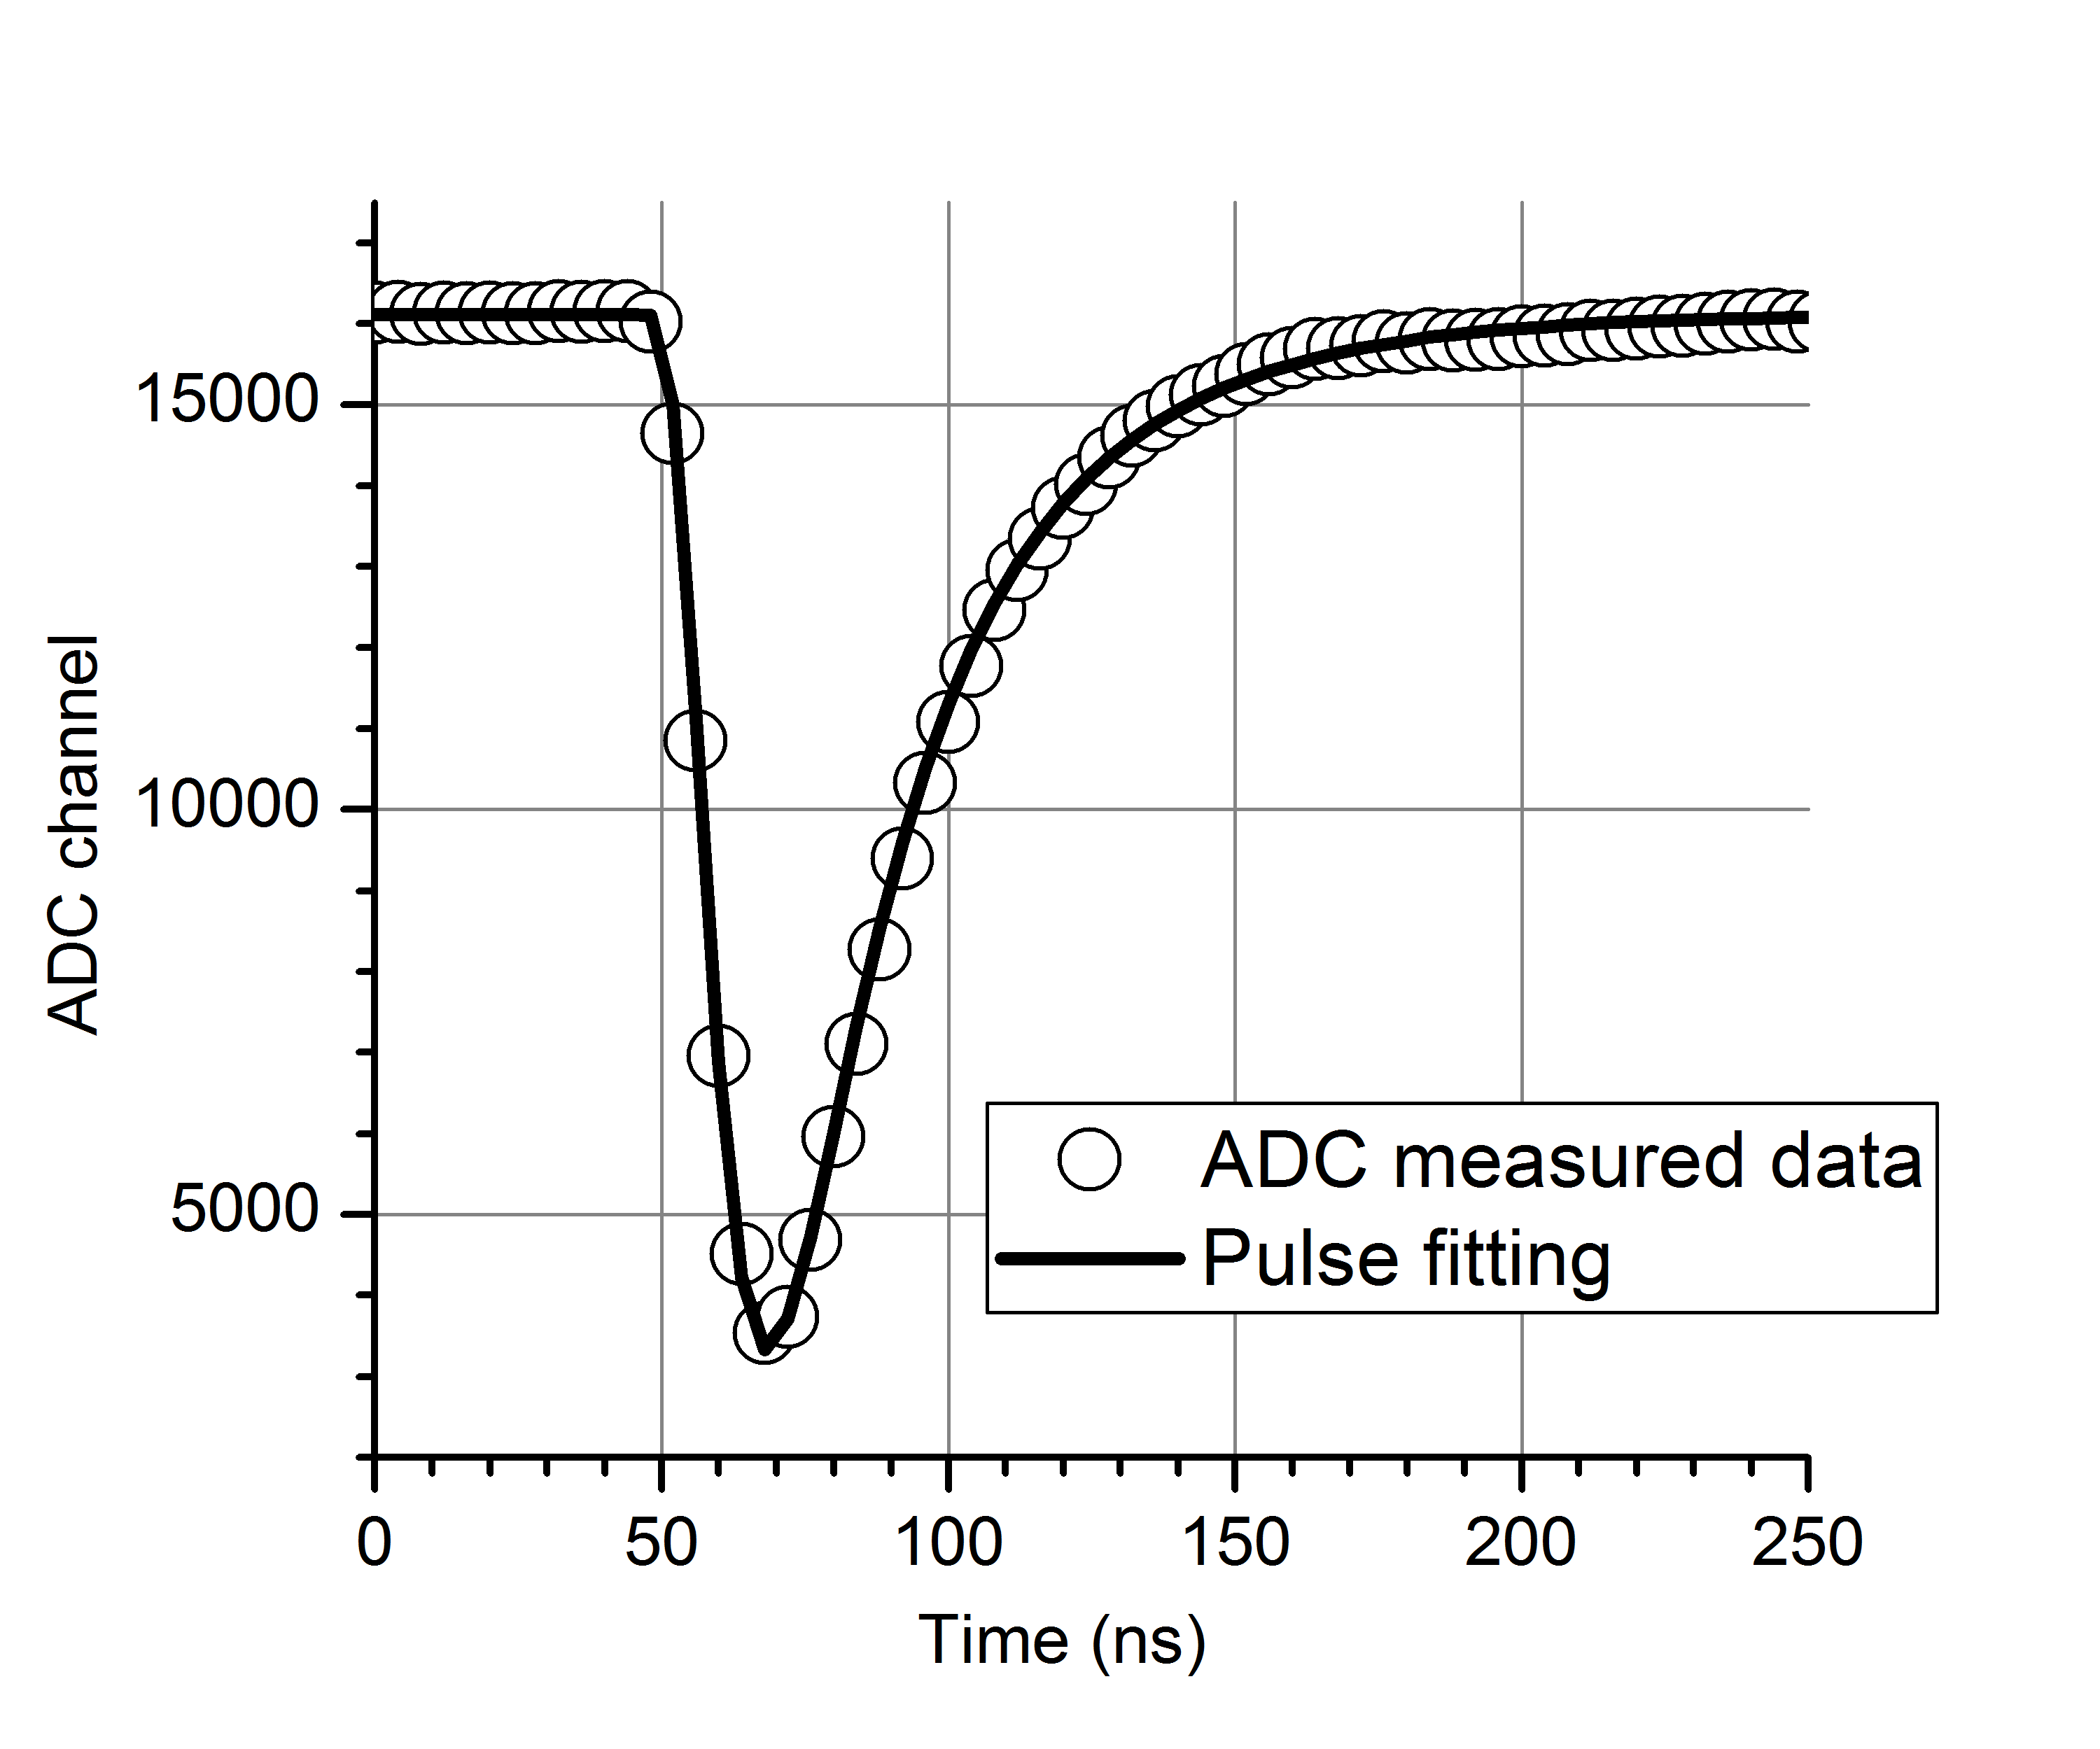
\includegraphics[width=0.60\linewidth]{pulseShapeFt2} }
  \caption{ Единчиный импульс, зарегистрированный детектором LaBr3(Ce) во время измерений на токамаке ФТ-2, а так же его аппроксимация аналитической формулой~\cite{Khilkevitch2020}.}
  \label{fig:pulseShapeFt2}
\end{figure}

\begin{figure}[ht!]
  \centerfloat{ 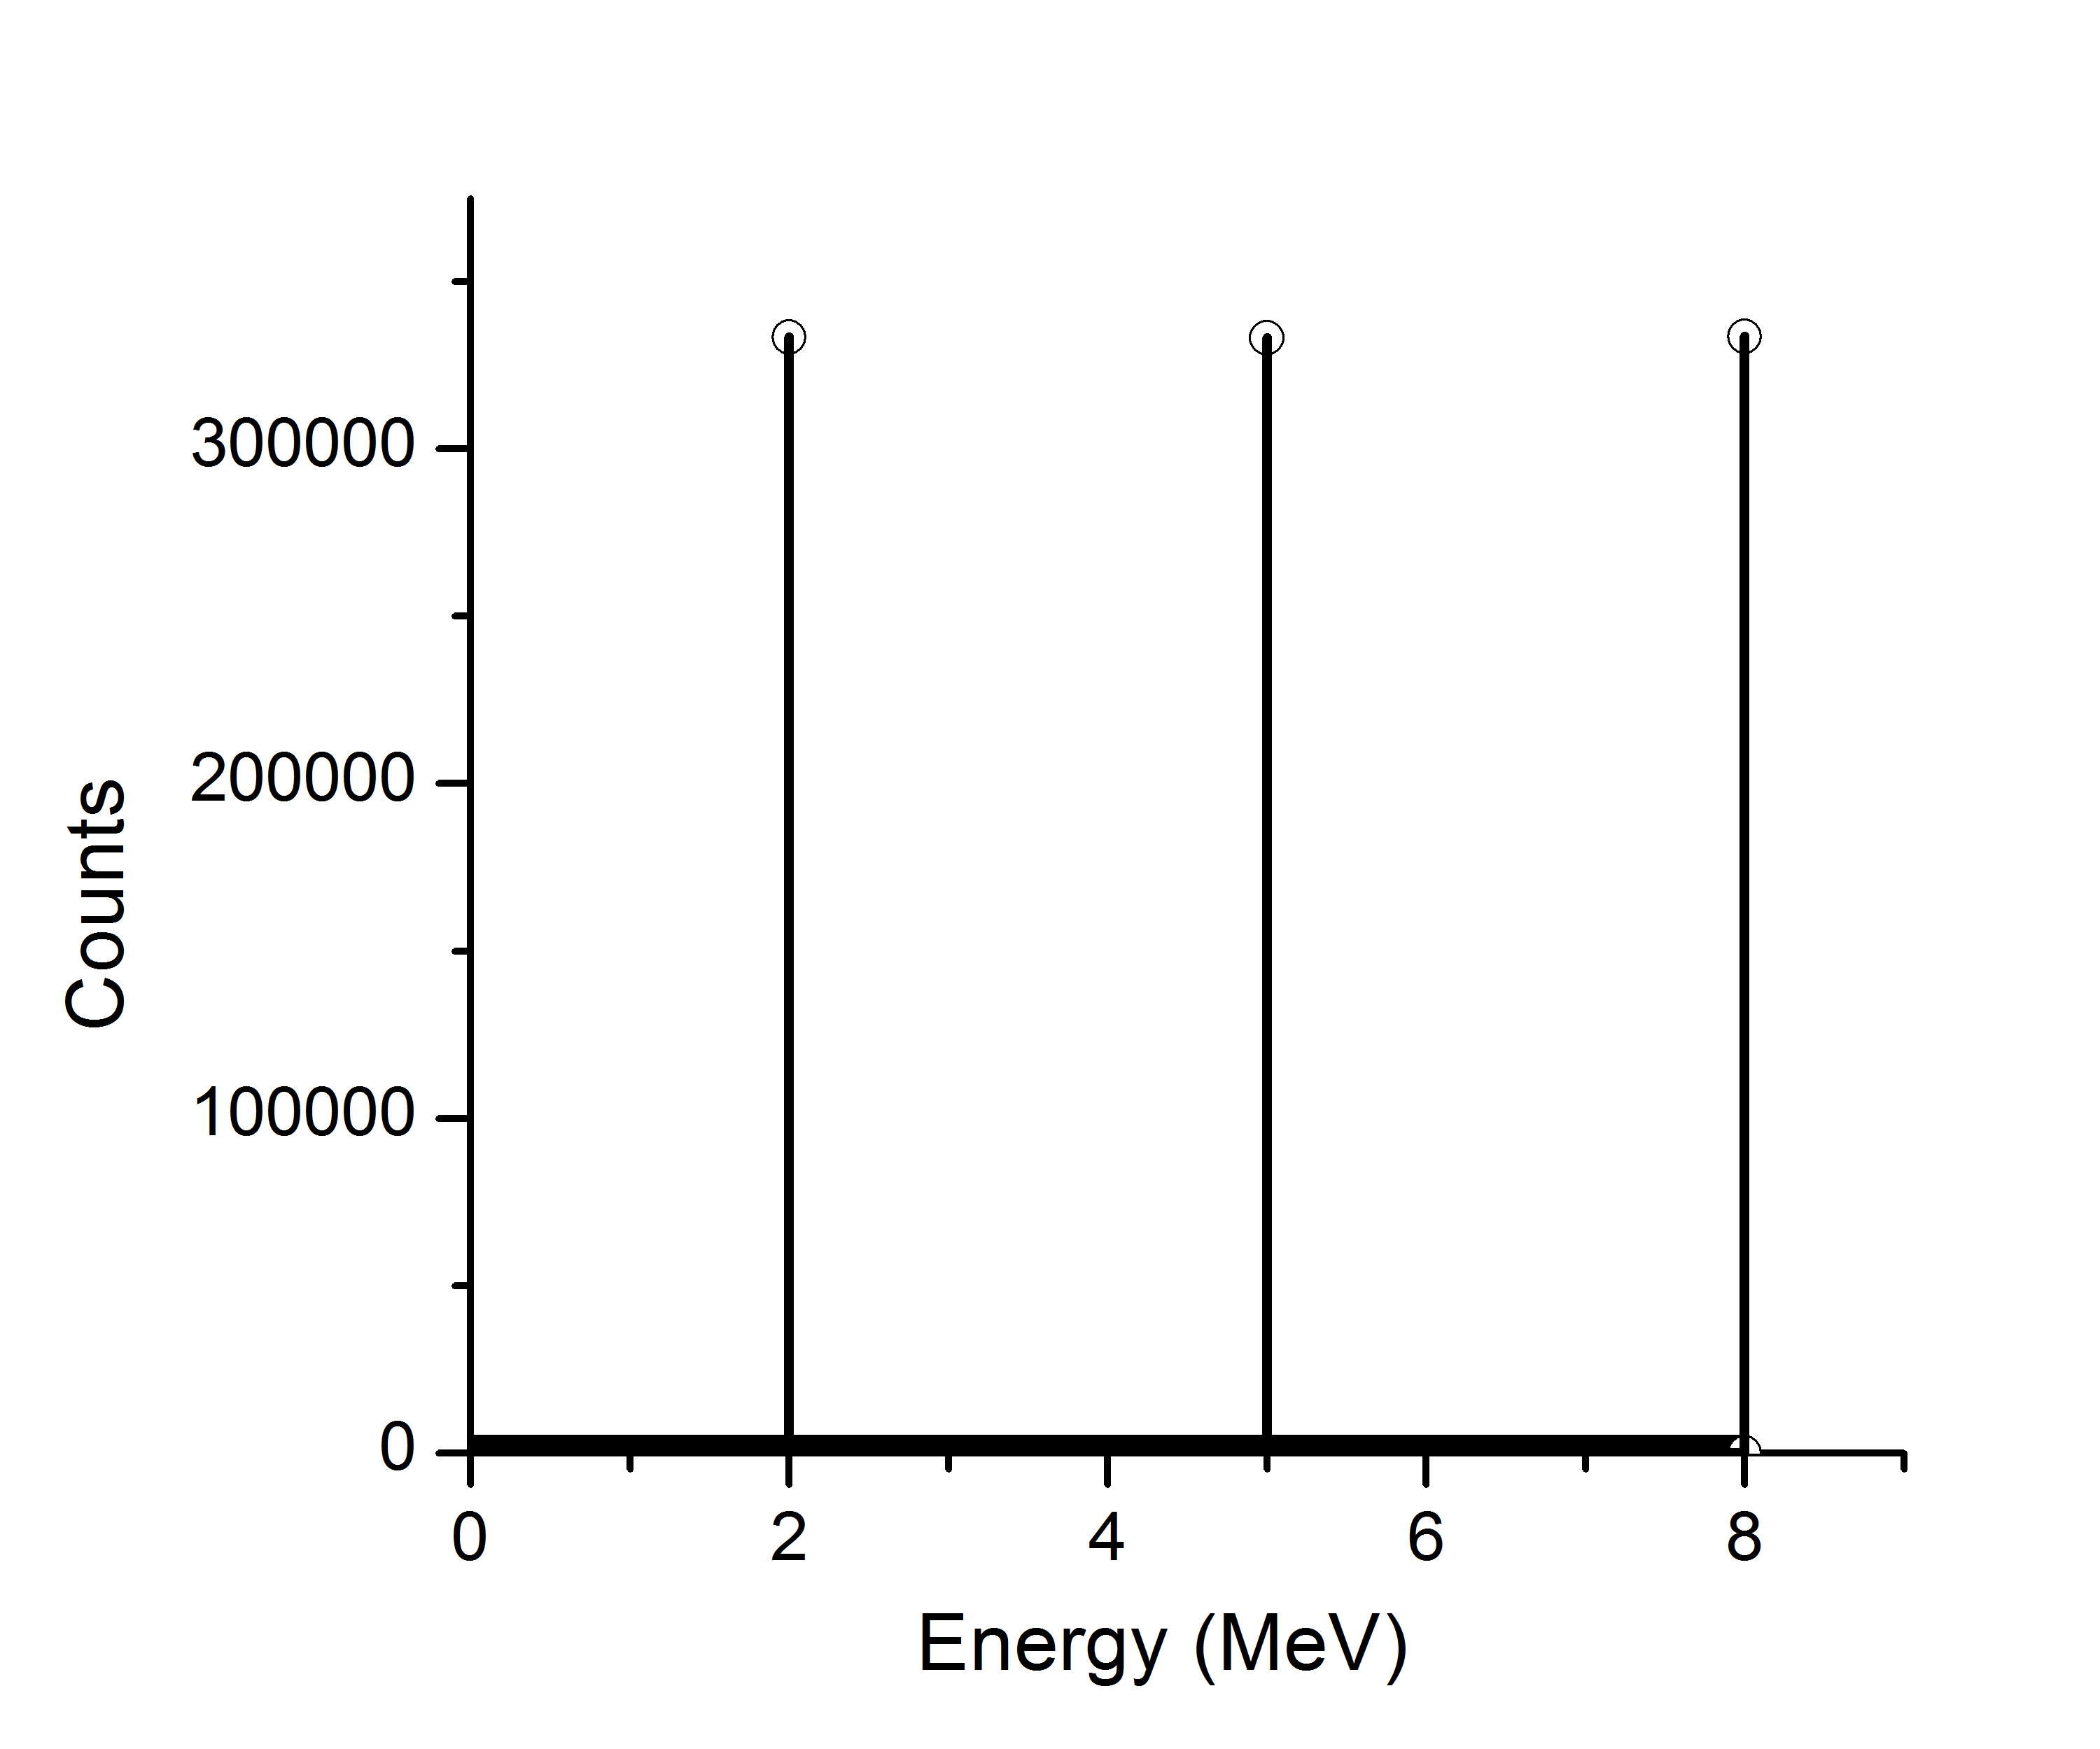
\includegraphics[width=0.60\linewidth]{testModelSpectrum} }
  \caption{ Распределение событий по энергии, которое использовалось при создании модельных сигналов~\cite{Khilkevitch2020}.}
  \label{fig:testModelSpectrum}
\end{figure}

\begin{figure}[ht!]
  \centerfloat{ 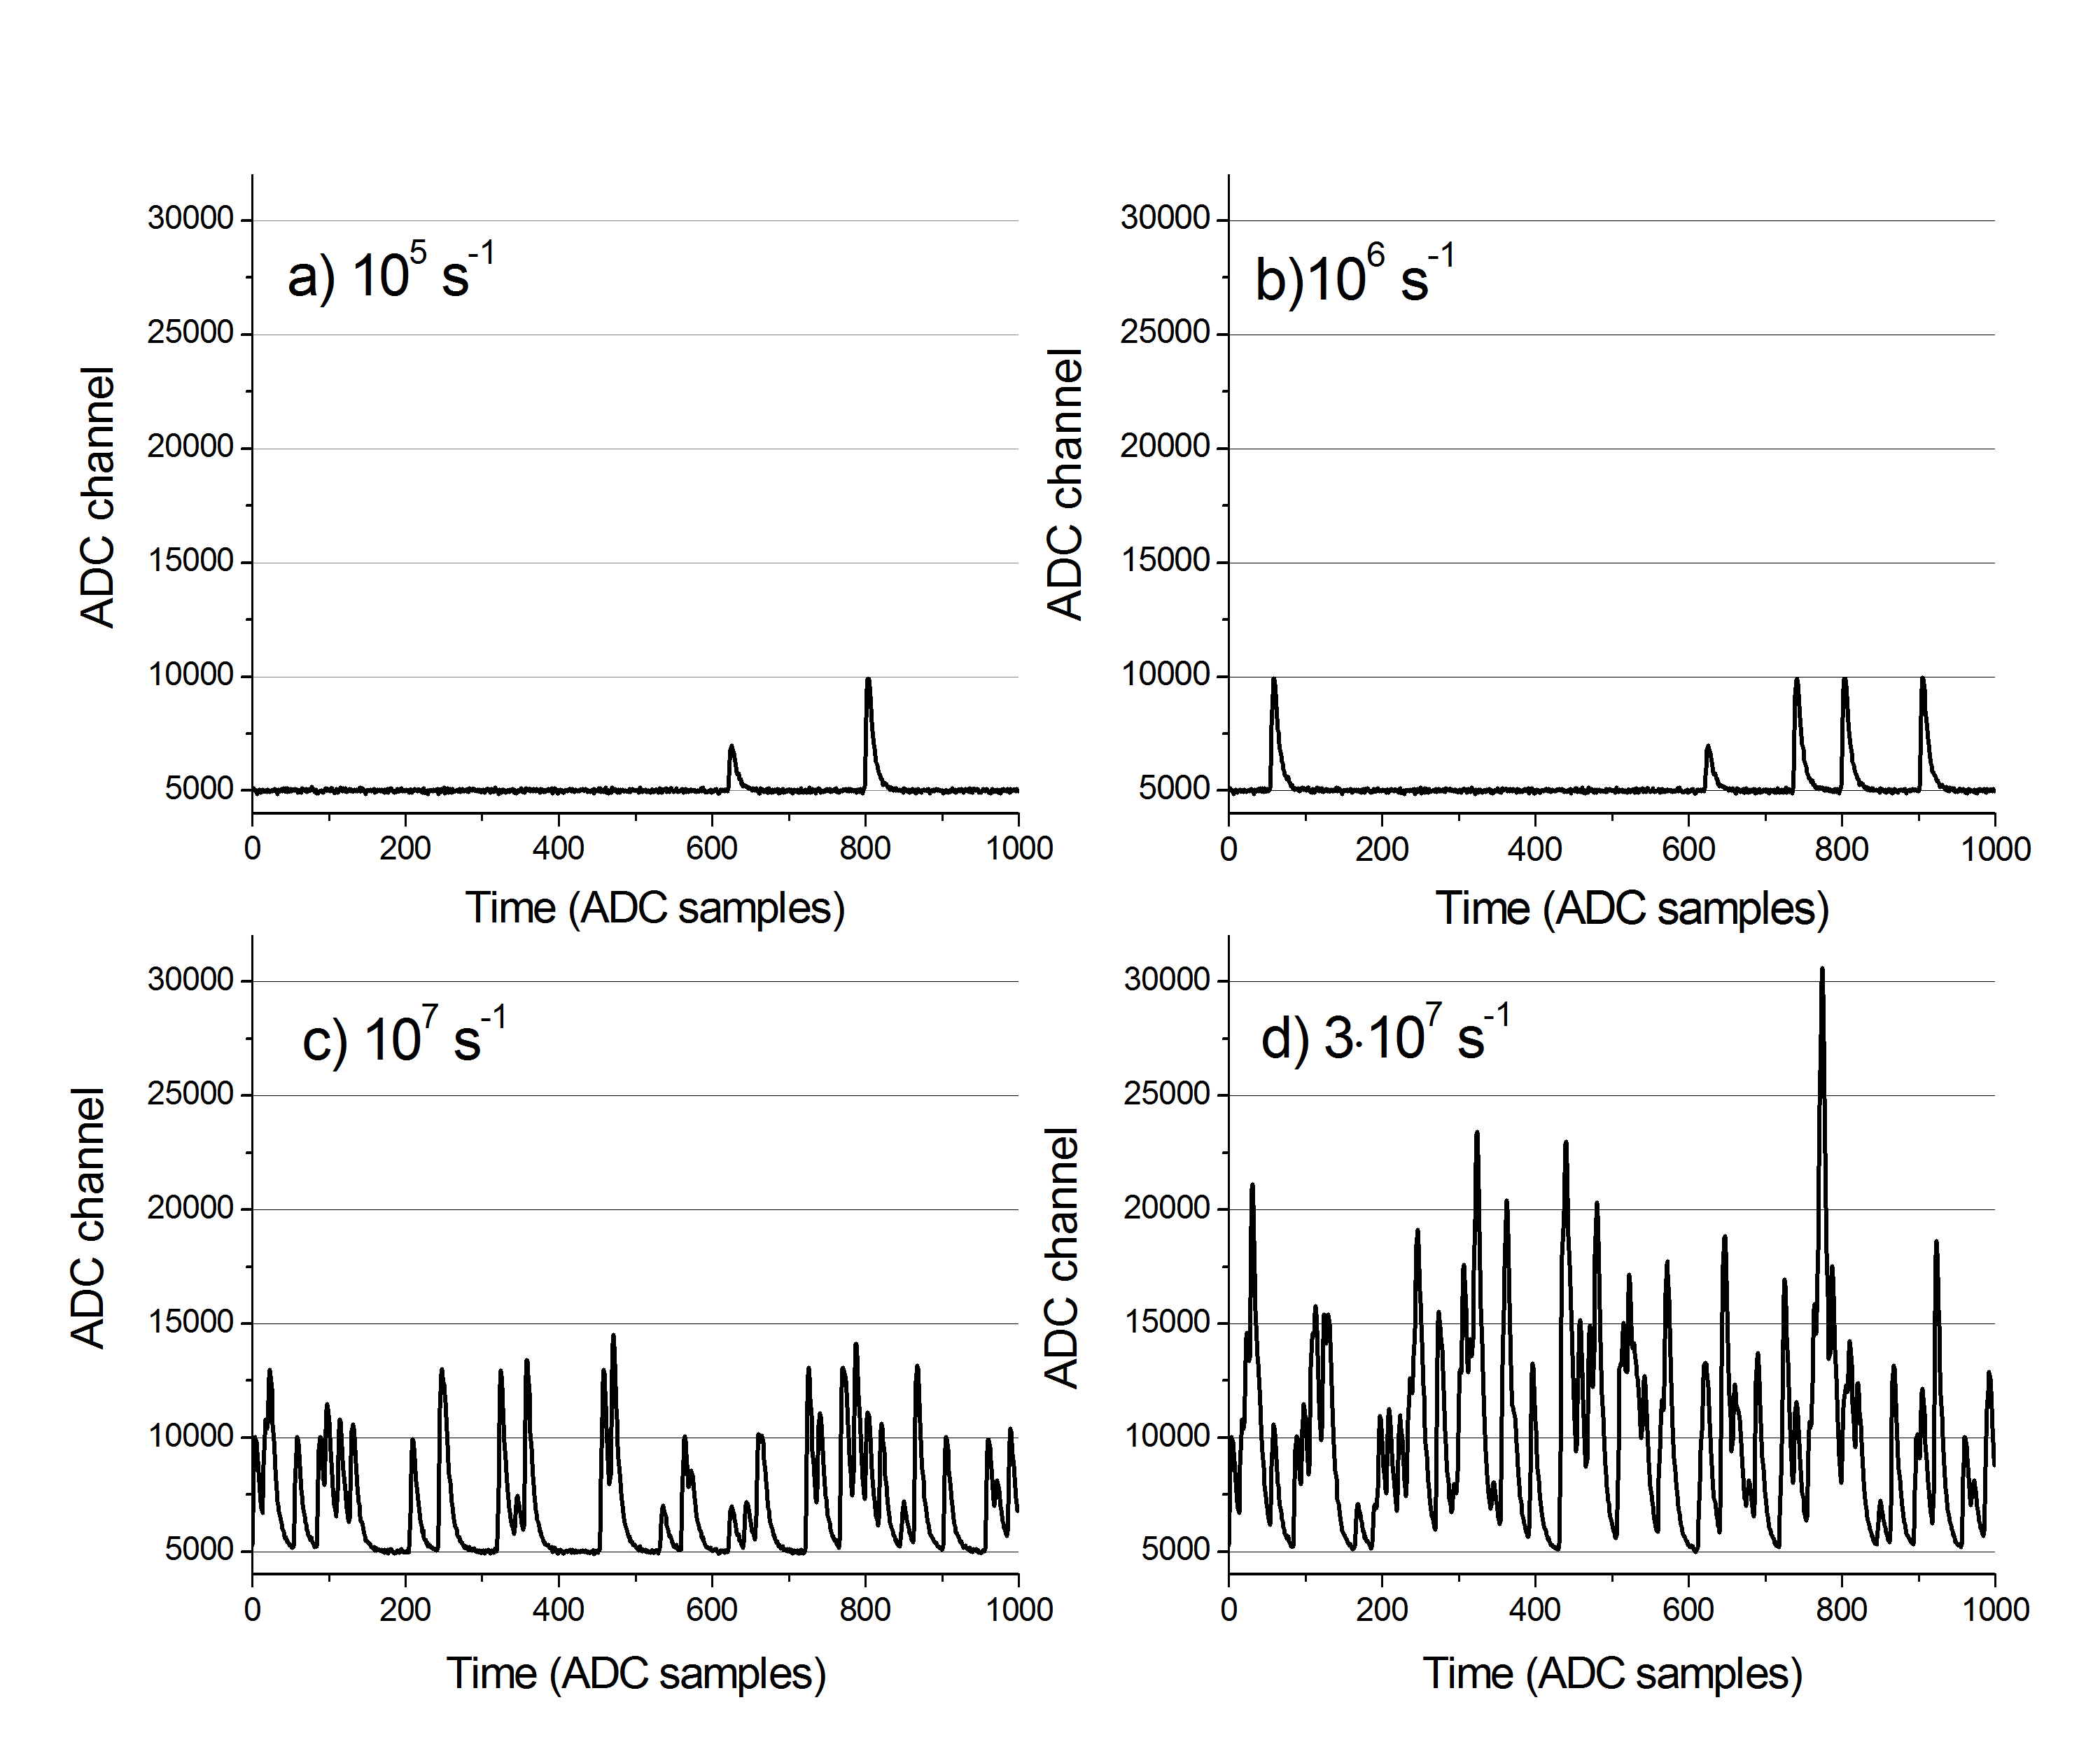
\includegraphics[width=0.96\linewidth]{testModelSignal} }
  \caption{ Модельные сигналы с разной скоростью счета: $10^5$~с${}^{-1}$~(a), $10^6$~с${}^{-1}$~(b), $10^7$~с${}^{-1}$~(c), $3\times10^7$~с${}^{-1}$~(d). При генерации использовалось одинаковое начальное значение генератора случайных чисел, поэтому по мере увеличения нагрузки в осциллограмму добавлялись новые события, а существующие события сохранялись.~\cite{Khilkevitch2020}.}
  \label{fig:testModelSignal}
\end{figure}

Для тестирования был сгенерирован набор модельных сигналов со скоростями счета $10^5$, $10^6$, $3\times10^6$, $10^7$, $2\times10^7$ и $3\times10^7$ импульсов в секунду (с${}^{-1}$). Моделирование проводилось для сигналов длительностью $t_{max} = 0.1$~с, генерируемых с частотой дискретизации 250~МГц. Использовался шум с гауссовым распределением $\sigma_n = 50$ и постоянным базовым значением $z = 5000$. События были случайным образом распределены во времени. Тестовые сигналы были откалиброваны для 1000~отчётов АЦП, соответствующих энергии гамма-излучения 1~МэВ --- по порядку величины это близко к реально используемым параметрам детектора (так, для детектора на токамаке ФТ-2 калибровка составляет примерно 1800 отсчётов на 1~МэВ). При калибровке полный диапазон энергий, измеряемый 14-разрядным АЦП, равнялся 16~МэВ. Это значение примерно соответствовало типичным параметрам, выбранным для измерения на токамаках ФТ-2 \cite{Shevelev2016,Shevelev2017} и Туман-3М \cite{Shevelev2018}. Сигналы генерировались с дискретным распределением амплитуды, показанным на рисунке~\ref{fig:testModelSpectrum}. Модельные сигналы для различных нагрузок показаны на рисунке~\ref{fig:testModelSignal}.  \cite{Khilkevitch2020}

% ==========================================================

\section{Определение нулевого уровня}

Определение нулевого уровня сигнала необходимо для дальнейшего применения методов обработки сигнала. Метод определения базовой линии должен работать при высоких скоростях счета, когда значение сигнала обычно $s(t) \gg z + n(t)$. Если значение нулевой линии во время измерения изменяется незначительно, можно использовать заданное вручную постоянное значение нулевой линии или, при обработке сигнала разряда токамака, нулевую линию можно определить автоматически в начале сигнала при низкой нагрузке детектора. Однако на практике значение нулевой линии в некоторых ситуациях существенно меняется во время разряда, например, из-за медленных периодических наводок от различного оборудования токамаков. В этом случае необходимо проводить периодические коррекции значения нулевой линии, и определять его динамически.

Целесообразно не искать значение нулевой линии в каждой точке сигнала, а ограничится периодическим определением этого значения через каждые $N_{zp}$ отсчетов АЦП. Это сокращает время обработки и позволяет отслеживать медленные изменения нулевой линии с характерным временем изменения $t_z \gg N_{zp}$. Для определения нулевого уровня можно использовать отдельные интервалы, выборки сигнала размером $N_{zd} \le N_{zp}$ в начале каждого интервала из $N_{zp}$ точек. В интервале $( k \cdot N_{zp} + N_{zd} ) \ldots ((k + 1) \cdot N_{zp})$, где $k$ --- номер интервала из точек $N_{zp}$, можно считать значение нулевой линии таким же, как и в ближайшем к нему интервале, на котором происходило вычисление значения нулевой линии. \cite{Khilkevitch2020}

% ----------------------------------------------------------

\subsection{Среднее значение и медиана}

Самый простой способ определения нулевой линии --- вычислить среднее значение:
\begin{equation*}
  z_{avg} = \frac{1}{N_{zd}} \sum\limits_{i = k \cdot N_{zp}}^{  k \cdot N_{zp} + N_{zd} } s_i 
\end{equation*}
Однако при высоких загрзуках полученное таким образом значение оказывается сильно смещено при высокой загрузке детектора (это верно для униполярного сигнала; если на АЦП приходит биполярный сигнал и $ \int_{-\infty}^{+\infty} p(t) dt = 0 $, то среднее значение вполне адекватно описывает значение нулевой линии).  

Второй очевидный способ вычисления значения нулевой линии --- это медиана, то есть такое число $z_{med}$, что половина значений сигнала $s_i$ в интервале $(k \cdot N_{zp}) \ldots (k \cdot N_{zp} + N_{zd})$ больше него, а вторая половина --- меньше. Такой сопосб вычисления нулевого уровня меньше подвержен эффекту смещения, однако всё равно даёт неудовлетворительные результаты при скорости счёта $10^7$~с${}^{-1}$ и выше. \cite{Khilkevitch2020}

% ----------------------------------------------------------

\subsection{Среднее значение по выборке}

Хороший результат дает объединение среднего и медианы в следующем итерационном алгоритме, который можно назвать <<среднее по выборке>> (<<аveraging over the selection set>>). Для неупорядоченного множества значений отсчетов $P_e$, изначально включающего в себя все значения отсчетов $s_i$ в интервале $(k \cdot N_{zp}) \ldots (k \cdot N_{zp} + N_{zd})$ определяются среднее арифметическое значение $z_{avg}$ и медиана $z_{med}$. Если 
\begin{equation}
  \label{eq:AvgOverSetCondition}
  | z_{avg} - z_{med} | < \delta z
\end{equation}
где $\delta z$ --- минимальная разность (значение этой величины является параметром алгоритма), то среднее арифметическое $z_{avg}$ можно считать равным значению нулевой линией. Типичное значение $\delta z$ составляет $0.1$--$1$; меньшие значения увеличивают время работы, при этом точность определения базовой линии с помощью алгоритма является избыточной, а большие значения приводят к недостаточной точности определения базовой линии. 

Если же условие~\ref{eq:AvgOverSetCondition} оказывается не выполненным, то из набора $P_e$ удаляются <<лишние>> значения. Количество удаляемых значений составляет $\max( \rho |P_e|, 1 )$, где $|P_e|$ --- число значений в множестве $P_e$, а величина $0 < \rho < 1$ является параметром алгоритма, обычно $\rho = 0.2$. Если $z_{avg} > z_{med}$ то из набора $P_e$ удаляются самые большие значения, а если  $z_{avg} < z_{med}$ --- то самые маленькие. После чего опять происходит вычисление $z_{avg}$ и $z_{med}$ для уменьшенного набора, и проверяется критерий~\ref{eq:AvgOverSetCondition}. Процедура повторяется до тех пор, пока этот критерий не будет выполнен. Алгоритм завершается за конечное число итераций, потому что на каждом шаге число значений в множестве $P_e$ уменьшается, а при $|P_e| = 1$ условие~\ref{eq:AvgOverSetCondition} оказывается выполнено автоматически. \cite{Khilkevitch2020}

Заметим, что для сигнала без событий $z_{avg} \approx z_{med}$. Регистрируемые события приводят к тому, что значения $z_{avg}$ и $z_{med}$ начинают смещаться от значения нулевой линии (для положительных импульсов --- в большую сторону, для отрицательных --- в меньшую). Величина смещения различается: среднее значение смещается больше, чем медиана. В данном алгоритме на каждом шаге из набора значений $P_e$ удаляются значения, вызывающие наибольшее смещение, то есть вершины импульсов. После удаления таких значений величины $z_{avg}$ и $z_{med}$ оказываются ближе к истинному значению нулевой линии. 

Работа алгоритма для участка модельного сигнала показана на рисунке~\ref{fig:baselineMethodAvgOverSet}. На первой итерации вычисления происходят для всех точек, $z_{avg} = 6921$, $z_{med} = 5969$. На второй итерации отбрасывается 20\% точек сигнала с самыми большими значениями, $z_{avg} = 5972$, $z_{med} = 5489$ --- значения стали ближе друг к другу и ближе к истинному значению нулевой линии. На третьей итерации отбрасывается ещё 20\% точек сигнала с самыми большими значениями, $z_{avg} = 5258$, $z_{med} = 5141$. На восьмой итерации $z_{avg} = 5013.02$, $z_{med} = 5013.0$, то есть значения $z_{avg}$, $z_{med}$ почти совпали; для $\delta z = 0.2$ алгоритм сходится за 8~итераций для данного участка сигнала.~\cite{Khilkevitch2020}

\begin{figure}[ht!]
  \centerfloat{ 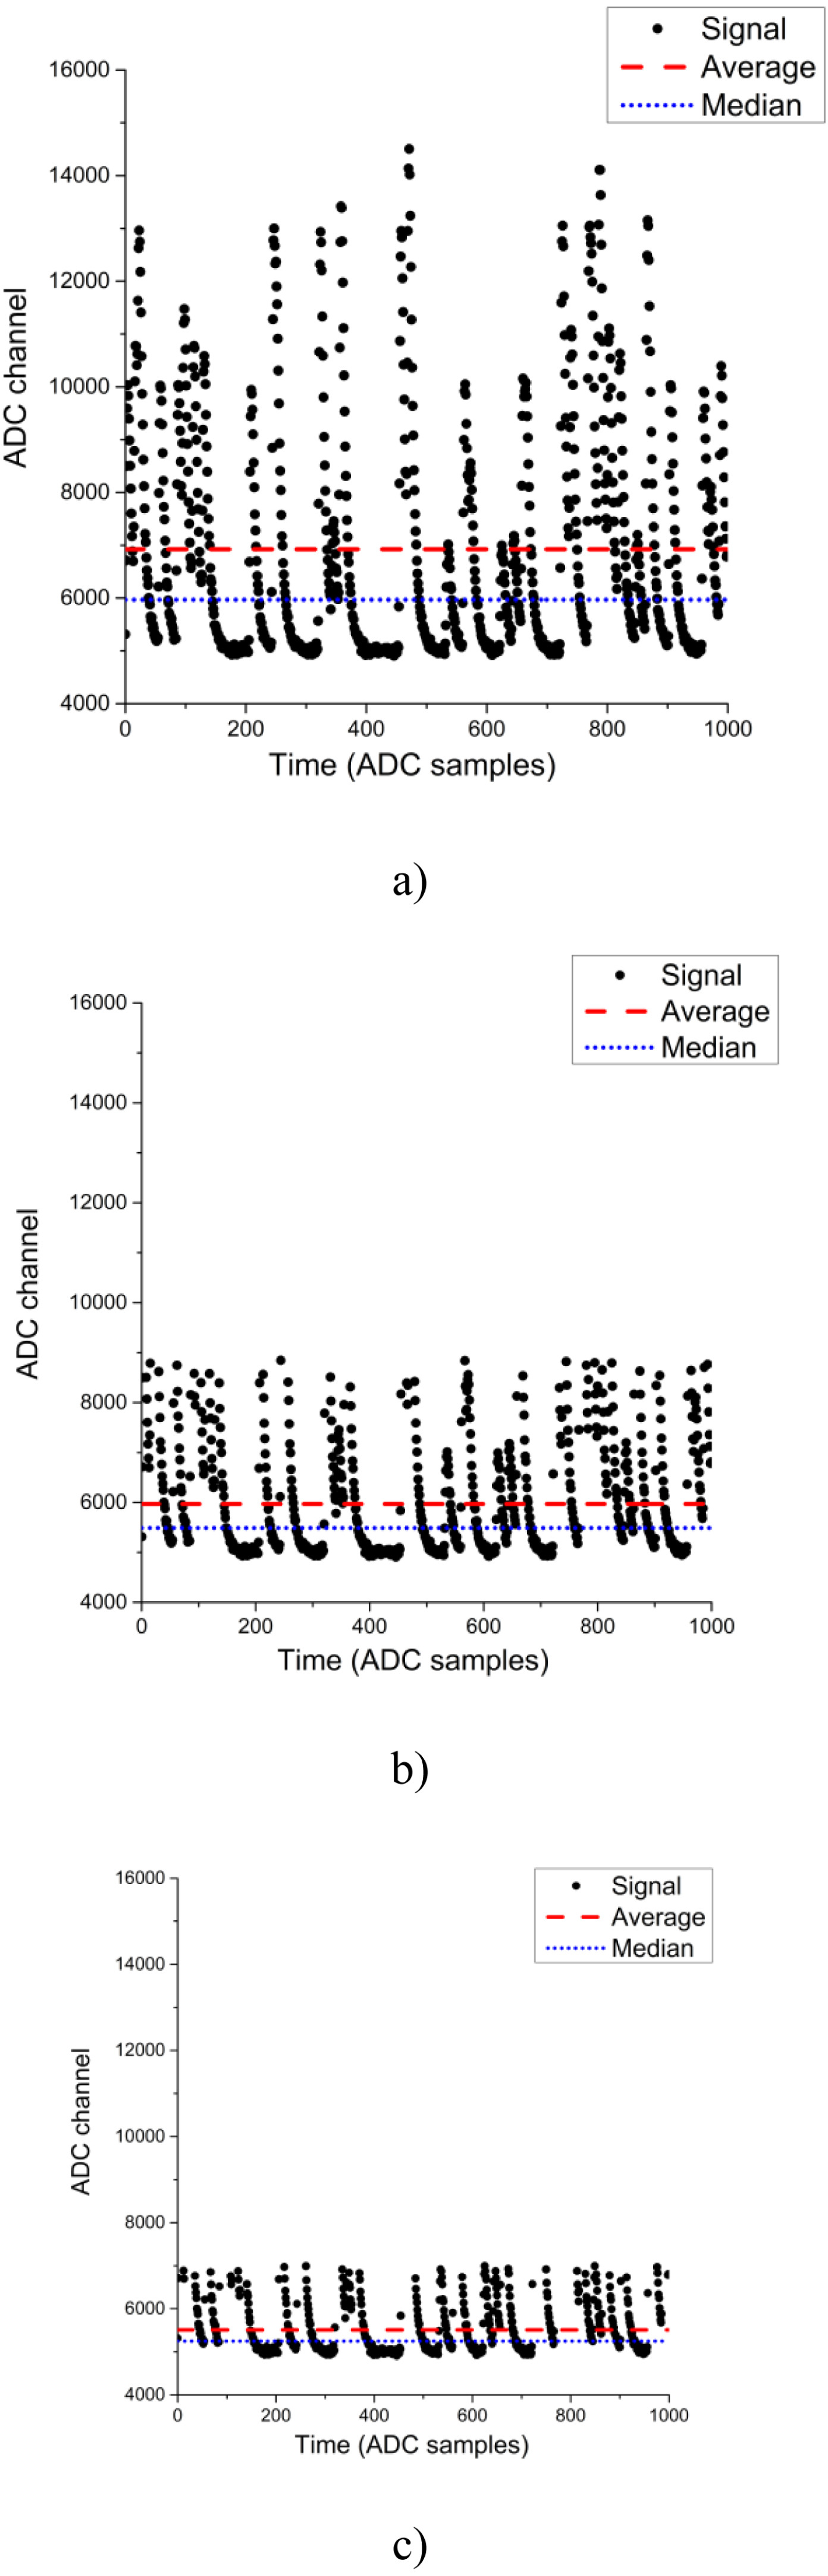
\includegraphics[width=0.40\linewidth]{baselineMethodAvgOverSet} }
  \caption{ Работа алгоритма <<среднее по выборке>> на примере участка модельного сигнала длиной 1000~точек с загрузкой $10^7$~с${}^{-1}$. Значение нулевой линии равно 5000. Чёрными точками обозначен сигнал, красным пунктиром --- среднее значение, синий линией --- медианное значение. Показаны первые три итерации алгоритма (рисуики а--в).~\cite{Khilkevitch2020}}
  \label{fig:baselineMethodAvgOverSet}
\end{figure}

% ----------------------------------------------------------

\subsection{Среднее значение по выборке плоских участков сигнала}

Описанный выше алгоритм <<среднего по выборке>> можно усовершенствовать, если из сигнала предварительно выделить плоские фрагменты (т.е. области, на которые не попадает значимый уровень сигнала от импульсов). Для этого в исходный набор данных $P_e$ для алгоритма включаются только те отсчеты $i$, для которых выполнены условия
\begin{equation}
  \label{eq:baselineMethodAvgOverFlatSet}
  \left|  s_i - \frac{1}{N_w} \sum \limits_{j=i-N_w}^{i-1} s_j  \right| < r, \hspace{5mm}
  \left|  s_i - \frac{1}{N_w} \sum \limits_{j=i+1}^{i+N_w} s_j  \right| < r 
\end{equation}
где $r$ --- пороговое значение (параметр алгоритма, выбранное типичное значение, которое больше уровня шума, но меньше чем характерный интервал между точками на фронте импульса), $N_w$ --- размер плоского участка импульса (параметр алгоритма, типичное значение 3--10), $N_w \ll N_{zd}$. Таким образом, в выборку попадают только значения таких точек, где значение сигнала лишь немного (на величину $r$) отличается от среднего уровня впереди и позади него, то есть только отсчеты, расположенные на достаточно ровных участках сигнала длительностью не более $2 \cdot N_w$. Затем к множеству таких значений применяется описанный выше алгоритм <<среднего по выборке>>. Этот метод можно назвать <<средним по выборке плоских участков>> (<<averaging over the flat chunk selection set>>). Иллюстрация работы алгоритма представлена на рисунке~\ref{fig:baselineMethodAvgOverFlatSet}.~\cite{Khilkevitch2020}

\begin{figure}[ht!!]
  \centerfloat{ 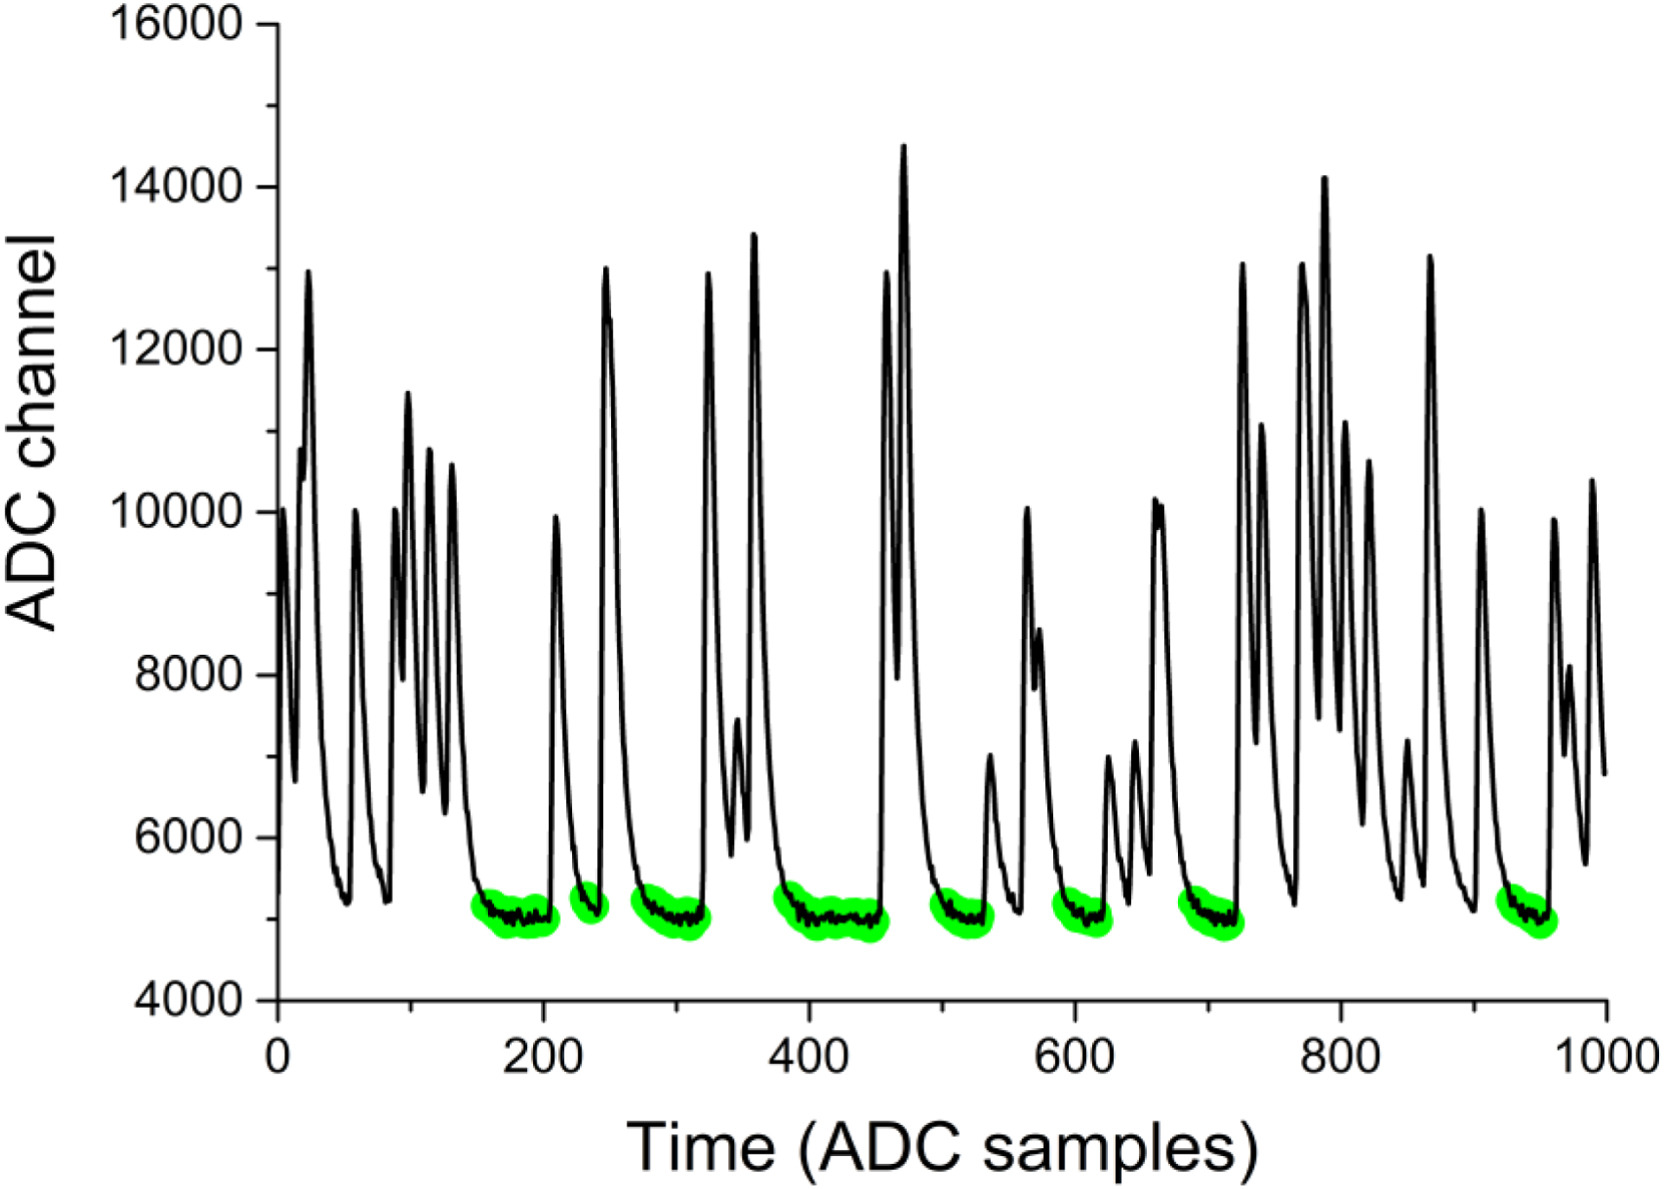
\includegraphics[width=0.50\linewidth]{baselineMethodAvgOverFlatSet} }
  \caption{ Работа алгоритма <<среднее по выборке плоских участков>> на примере участка модельного сигнала длиной 1000~точек с загрузкой $10^7$~с${}^{-1}$. Значение нулевой линии равно 5000. Чёрными точками обозначен сигнал, зелёным подсвечены участки сигнала, точки в которых удовлетворяют критерию~\ref{eq:baselineMethodAvgOverFlatSet}.~\cite{Khilkevitch2020}}
  \label{fig:baselineMethodAvgOverFlatSet}
\end{figure}

% ----------------------------------------------------------

\subsection{Сравнение методов определения значения нулевой линии}

Сравнение описанных выше методов показано на рисунке~\ref{fig:baselineMethodsComparison} при разных значениях скорости счета. Ошибка определения базовой линии равна абсолютной величине разницы между известным сгенерированным значением базовой линии модельного сигнала ($z = 5000$) и значением, полученным с помощью описанных выше алгоритмов. Наилучшие результаты демонстрирует алгоритм <<среднее по выборке плоских участков>>. При загрузке детектора $3 \times 10^7$ с${}^{-1}$ и выше погрешности определения базовой линии оказываются неприемлемо велики для всех алгоритмов, так как погрешность определения нулевой линии превышает 200 отсчётов при использовании любого рассмотренного алгоритма для выбранных событий. Это происходит из-за того, что при настолько значительной скорости счёта детектора в осциллограмме почти нет участков, где значение сигнала равно $s(t) \approx z + n(t)$ без влияния импульсов от регистрации гамма квантов.

\begin{figure}[ht!]
  \centerfloat{ 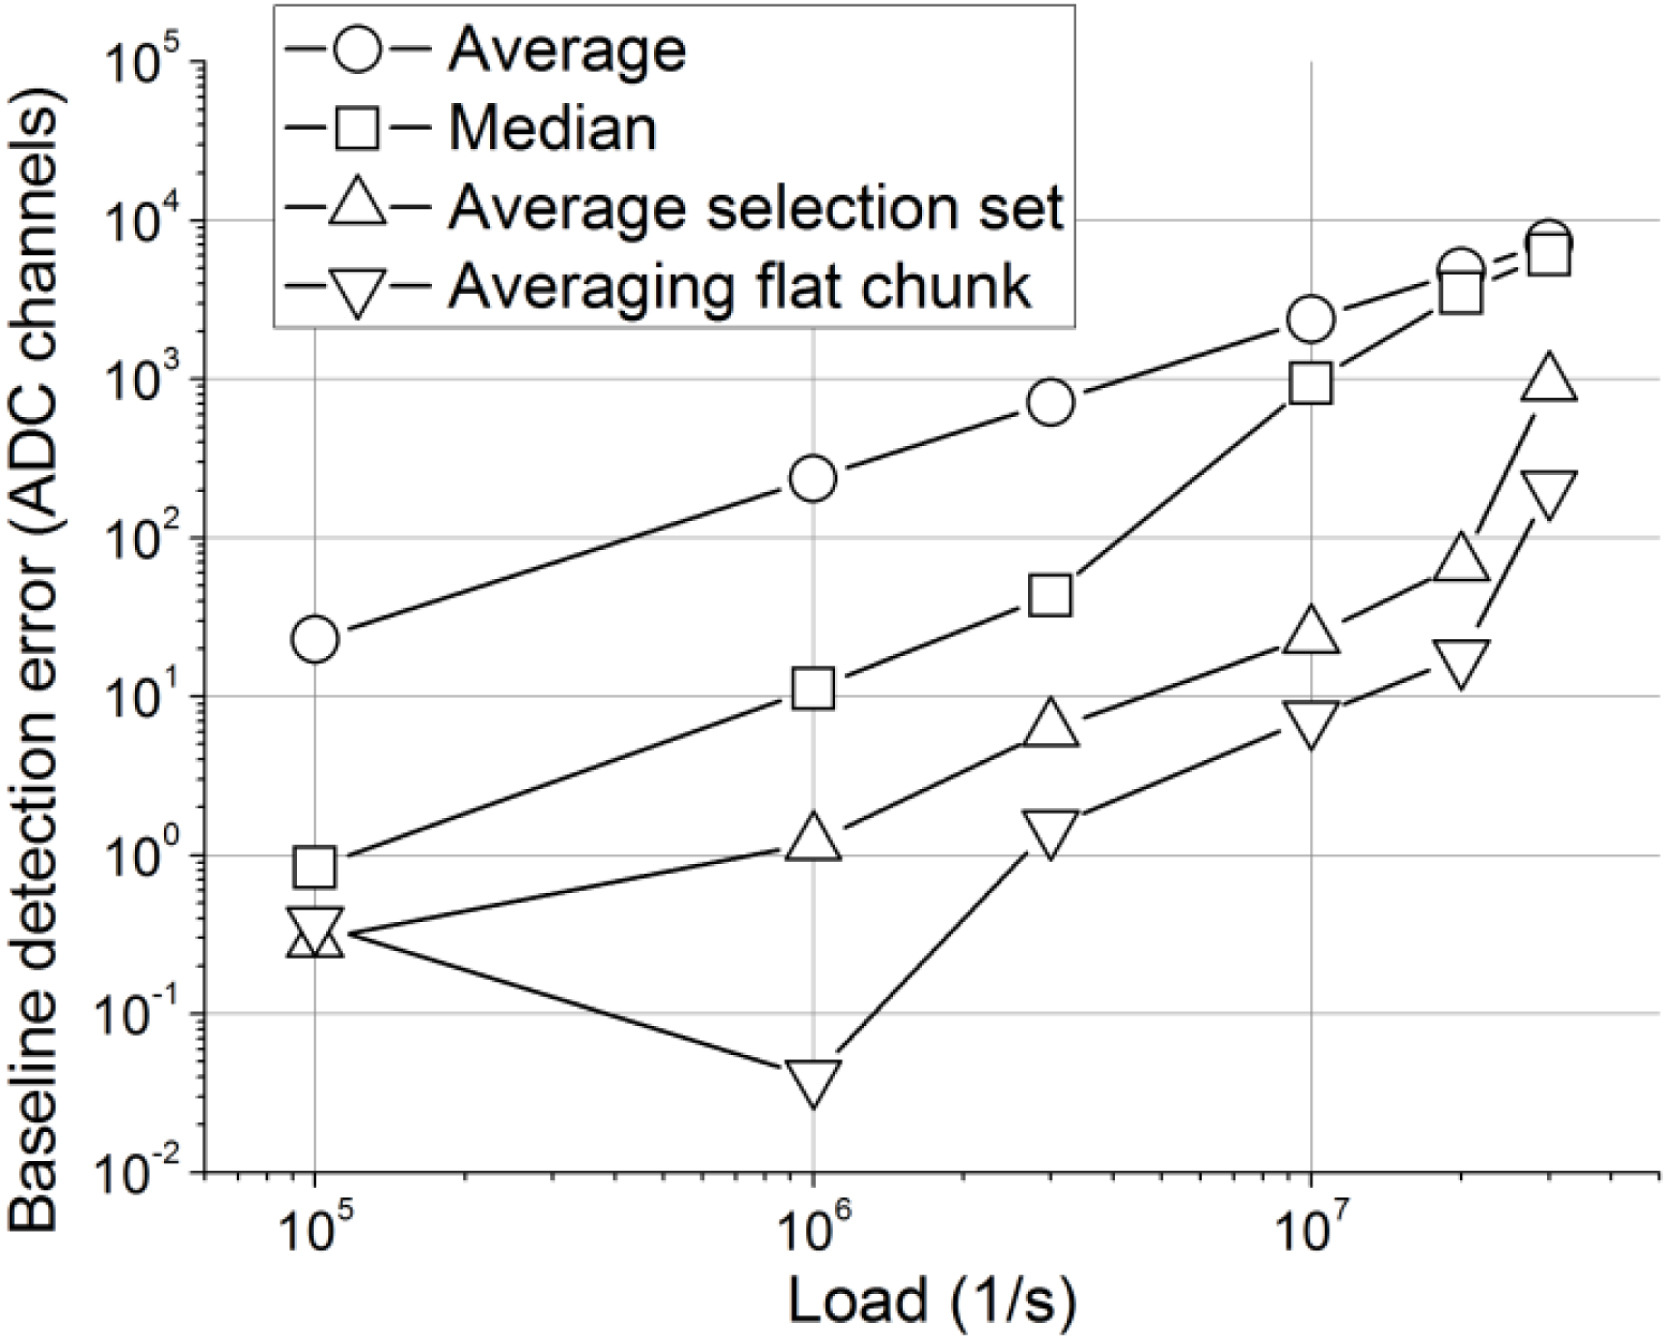
\includegraphics[width=0.60\linewidth]{baselineMethodsComparison} }
  \caption{ Ошибка в определении базового значения, полученного для различных нагрузок с использованием различных алгоритмов. По оси~Y показана ошибка в каналах АЦП модельного сигнала. Параметры алгоритмов: $N_{zd} = 10000$, $\delta z = 0.2$, $N_w = 10$, $r = 30$.  Немонотонное поведение ошибок алгоритма <<средним по выборке плоских участков>> объясняется случайными флуктуациями. В немонотонной области значение ошибки составляет менее $0.01$ отсчетов АЦП и пренебрежимо мало на практике.~\cite{Khilkevitch2020}}
  \label{fig:baselineMethodsComparison}
\end{figure}

\FloatBarrier

% ==========================================================

\section{Определение амплитуд и времени регистрации гамма квантов}

Перед определением амплитуд и времени регистрации импульсов из сигнала $s(t)$ вычитается значение нулевой линии $z$, определяемой по одному из ранее описанных алгоритмов. В дальнейшем будем считать, что определение и вычитание нулевой линии уже выполнено, поэтому $z = 0$. Предполагается, что форма импульса описывается известным уравнением и равна $p(t)$. Предполагается также, что $p(0) = 1$, $\forall t: p(t) \le p(0)$ --- импульс нормирован так, чтобы его максимальное значение было равно 1, и максимум достигался при значении $t = 0$. Для каждого события необходимо найти значения $t_j$ и $A_j$ из выражения~\ref{eq:OscShapeBase}.~\cite{Khilkevitch2020}

% ----------------------------------------------------------

\subsection{Максимальное значение}

Самый простой способ определить амплитуды событий --- найти максимальное значение импульса. Для сигнала $s_i$ необходимо найти все интервалы индексов $B_j \ldots E_j$, для которых которых $\forall i \in \left[ B_j \ldots E_j \right]: |s_j| > r$, где $r$ --- пороговое значение дискриминации. Также необходимо найти локальный максимум на каждом из этих интервалов. Это максимальное значение считается равным амплитуде события $A_j$, а время, при котором сигнал достигает локального максимума, равно времени регистрации события $t_j$.

Этот алгоритм прост и демонстрирует очень хорошую скорость обработки сигнала. Однако даже при небольшой нагрузке он обеспечивает посредственное определение истинных амплитуд импульсов, так как найденное значение чувствительно к шуму сигнала. Также из-за дискретности АЦП даже в сигнале без шумовой составляющей значение $t_j$, определённое таким образом, может отличаться на один отсчет от истинного значения времени регистрации сигнала и, соответственно, это приводит к ошибке определения амплитуды, поскольку в таком случае $ \max_{ti} p(t_i - t_j ) < 1 $. Кроме того, этот алгоритм не может адекватно определить амплитуды наложенных импульсов. Поэтому при больших загрузках определённые с помощью такого алгоритма значения $(t_j, A_j)$ будут значительно отличаться от истинных.~\cite{Khilkevitch2020}

% ----------------------------------------------------------

\subsection{Сумма}
\label{sec:ProcessingSum}

Для исключения влияния шума на результаты расчета амплитуды можно использовать и сумму отсчётов по импульсу в интервале:
\begin{equation*}
  S_j = \sum \limits_{i = B_j}^{E_j} s_i
\end{equation*}
Эта сумма зависит от того, какая часть импульса попадает в этот интервал: для импульса с большей амплитудой в интервал суммирования попадает больше точек. Поэтому имеет смысл использовать значение амплитуды импульса
\begin{equation*}
  A_j = \frac{ \sum\limits_{i=B_j}^{E_j} s_i }{ \sum\limits_{i=B_j}^{E_j} p( i - t_j ) }
\end{equation*}
где время регистрации события $t_j$ неизвестно. Приравнивание $t_j$ к времени достижения локального максимума не является точным из-за влияния возможного шума; кроме того, реальное время $t_j$ может иметь ненулевую дробную часть (т.е. событие произошло в промежутке времени между соседними сэмплами АЦП), а определённое таким образом значение заведомо является целым числом. Можно подобрать такое значение $t_j$, чтобы разность между положением центра масс измеряемого сигнала и единичной формой импульса $p(t)$ со сдвигом была минимальной:
\begin{equation*}
  \min \left( \left| \frac{ \sum \limits_{i = B_j}^{E_j} s_i \cdot (i - t_j^{max}) }{\sum \limits_{i = B_j}^{E_j} s_i} - 
                     \frac{ \sum \limits_{i = B_j}^{E_j} p( i - t_j ) \cdot (i - t_j^{max}) }{\sum \limits_{i = B_j}^{E_j} p(i - t_j) }   \right| \right) 
\end{equation*}
где $t_j^{max}$ --- время, при котором сигнал $s_i$ на интервале $\left[ B_j \ldots E_j \right] $ достигает максимального значения. 

Этот алгоритм также не может определять амплитуды наложенных импульсов. События, для которых 
\begin{equation}
  \label{eq:UnresolvedSumCrit}
  B_j - E_{j-1} < \delta i 
\end{equation}
где $\delta i$ --- параметр алгоритма (типичное значение около характерного времени спада импульса или чуть меньше), следует отбросить, так как для таких событий амплитуда второго события будет существенно искажена влиянием первого события: эти близкие события считаются неразрешёнными. Однако влияние неразрешённых событий также может быть учтено. Для таких неразрешенных событий можно оценить их суммарную амплитуду равной
\begin{equation}
  \label{eq:UnresolvedAmplitude}
  A_j^u = \frac{  \sum \limits_{i = B^u_j}^{E^u_j} s_i }{ \sum \limits_{i = -\infty}^{+\infty} p(i) }
\end{equation}
где $\left[ B_j^u \ldots E_j^u \right] $ --- объединённый интервал для всех соседних событий, не удовлетворяющих условию~\ref{eq:UnresolvedSumCrit}. Можно предположить, что распределение амплитуд неразрешенных событий примерно соответствует распределению разрешённых событий в их непосредственной близости. Для учета неразрешенных событий каждому событию присваивается вес $w_j$. При условии отсутствия неразрешённых событий этот вес изначально равен $1$ для всех событий. Однако если событие $j$ не разрешено (не соответствует критерию~\ref{eq:UnresolvedSumCrit}), то для каждого события в интервале $i_b \ldots i_e$ вблизи события $j$ этот вес увеличивается на величину
\begin{equation*}
  \Delta w = \frac{ A_j^u }{ \sum \limits_{i=i_b}^{i_e} A_i } 
\end{equation*}
Величину интервала $i_b \ldots i_e$ можно определять разными способами, например как $i_b = j - N_{uw}$, $i_e = j + N_{uw}$, где величина $N_{uw}$ --- параметр алгоритма, типичное значение, используемое нами, обычно равно 1000. При построении спектра значение в энергетическом интервале $i$ в диапазоне энергий $\varepsilon_i \ldots \varepsilon_{i+1}$ определяется как сумма
\begin{equation*}
  \sum_j w_j | \varepsilon_i \le A_j < \varepsilon_{i+1}
\end{equation*}
Аналогично при построении зависимости скорости счёта детектора от времени число событий во временном интервале $t_i \ldots t_{i+1}$ определяется как
\begin{equation*}
  \sum_j w_j | t_i \le t_j < t_{i+1}
\end{equation*}
Спектр, полученный этим методом, можно зазывать скорректированным спектром. Заметим, что построенный таким образом спектр, учитывающий неразрешённые значения, может содержать нецелые значения, в отличие от <<обычного>> спектра, где в каждом интервале содержится всегда целое число событий.~\cite{Khilkevitch2020}

% ----------------------------------------------------------

\subsection{Фиттинг по форме импульса}
\label{sec:FittingProcessing}

В качестве усовершенствованного метода определения амплитуды, обеспечивающего разделение наложенных импульсов, можно использовать подгонку (фиттинг) фрагмента осциллограммы известной формой импульса $p(t)$, в результате чего определить амплитуду и время регистрации события. Первоначальный метод был описан в \cite{Gin2008}, однако в \cite{Khilkevitch2020} он был модифицирован для повышения точности.

Будем для каждого события $j$ искать такие параметры $A_j$ и $t_j$, чтобы минимизировать невязку
\begin{equation}
  \label{eq:FittingResidual}
  R(t_j,A_j) =   \sum \limits_{i=B^f_j}^{E^f_j} \left| s'_i - A_j \cdot p( i - t_j ) \right|
\end{equation}
где $B^f_j < t_j^{max}$ и $E^f_j > t_j^{max}$ определяют интервал, в котором проводится фиттинг. Заметим, что эти значения не обязательно равны значениям $B_j$ и $E_j$. Значение 
\begin{equation*}
  s'_i = s_i - \sum \limits_{k=0}^{j-1} A_k \cdot p( i - t_k )
\end{equation*}
учитывает влияние медленно спадающих <<хвостов>> предыдущих импульсов при анализе импульса $j$. Поскольку сигнал обрабатывается последовательно, то все значения $A_k$ и $t_k$ для $k<j$ известны.

При заданном значении $t_j$ минимум невязки $R(A_j)$ может быть определён методом наименьших квадратов и равен
\begin{equation}
  \label{eq:FittingAmplitude}
  A_j = \frac{ \sum \limits_{i=B^f_j}^{E^f_j} s' \cdot p(i - t_j) }{ \sum \limits_{i=B^f_j}^{E^f_j} p^2(i-t_j) }
\end{equation}
Соответственно, необходимо найти такое значение $t_j$ на интервале $\left[ B_j \ldots E_j \right] $, такое чтобы чтобы невязка из выражения~\ref{eq:FittingResidual} со значением амплитуды их \ref{eq:FittingAmplitude} принимала наименьшее значение. Это можно сделать методом троичного поиска \cite{Scherer2017}, который, с одной стороны, работает достаточно быстро, а с другой стороны, обеспечивает достаточную для гамма-спектрометрии точность определения значения $t_j$ (обычно нам требуется знать $t_j$ с точностью не более долей единицы). Поиск ведется на дискретной сетке с шагом $1/t_v$, где целочисленное значение $t_v \ge 1$ (это параметр алгоритма, обычно используемые нами значения равны 2 или 4, оно определяется желаемой точностью определения $t_j$). Интервал поиска равен $ t_j^{max} - \Delta^b \ldots  t_j^{max} + \Delta^e$, где $\Delta^b$ и $\Delta^e$ --- параметры алгоритма, которые определяются шириной импульса и уровнем шума; обычно $\Delta^b = \Delta^e = 3..10$.

%Если для вычисленных значений  $A_j$ и $t_j$ невязка оказалась больше некоторого значения
%\begin{equation}
%  \label{eq:ResidualCondition}
%  R( A_j, t_j ) \ge R^{max}
%\end{equation}
%где  $R^{max}$ --- параметр алгоритма, обычно это значение в 2--3 раза больше уровня шума, то считается что импульс не удалось разрешить, так как его форма слишком сильно отличается от эталонной формы $p(t)$. В этом случае можно применить ту же коррекцию итогового спектра на неразрешённые импульсы, что была описана выше в разделе~\ref{sec:ProcessingSum}, и рассчитать суммарную амплитуду неразрешённых сигналов по той же формуле~\ref{eq:UnresolvedAmplitude}~\cite{Khilkevitch2020}.


Если значение невязки больше некоторого порогового значения 
\begin{equation*}
  \frac{ R(t_j,A_j) }{ E_j - B_j } > R^{max}
\end{equation*}
где $R^{max}$ --- параметр алгоритма, обычно это значение в 2--3 раза больше уровня шума, то предполагается, что форма импульса слишком сильно отличается от $p(t)$, а значения $A_j$ и $t_j$ определены неверно. Это может произойти из-за очень близкого наложения двух или более импульсов, так что хотя сигнал $s_i$ имеет только один локальный максимум в интервале $\left[ B_j \ldots E_j \right] $, но реально было зарегистрировано более одного события. В этом случае можно считать, что события не удалось разрешить. Однако и эти неразрешённые события можно учитывать так же, как и в разделе~\ref{sec:ProcessingSum}.


После определения времени и амплитуды события $j$ хвост импульса вычитается из остаточного сигнала перед его обработкой по формуле
\begin{equation*}
  s'_i = s_i - A_j \cdot p( t - t_j )
\end{equation*}
Эта процедура учитывает влияние события $j$ на последующие события.

Пример работы алгоритма показан на рисунке~\ref{fig:FittingProcessing}.

\begin{figure}[ht]
    \begin{minipage}[b][][b]{0.95\linewidth}\centering
        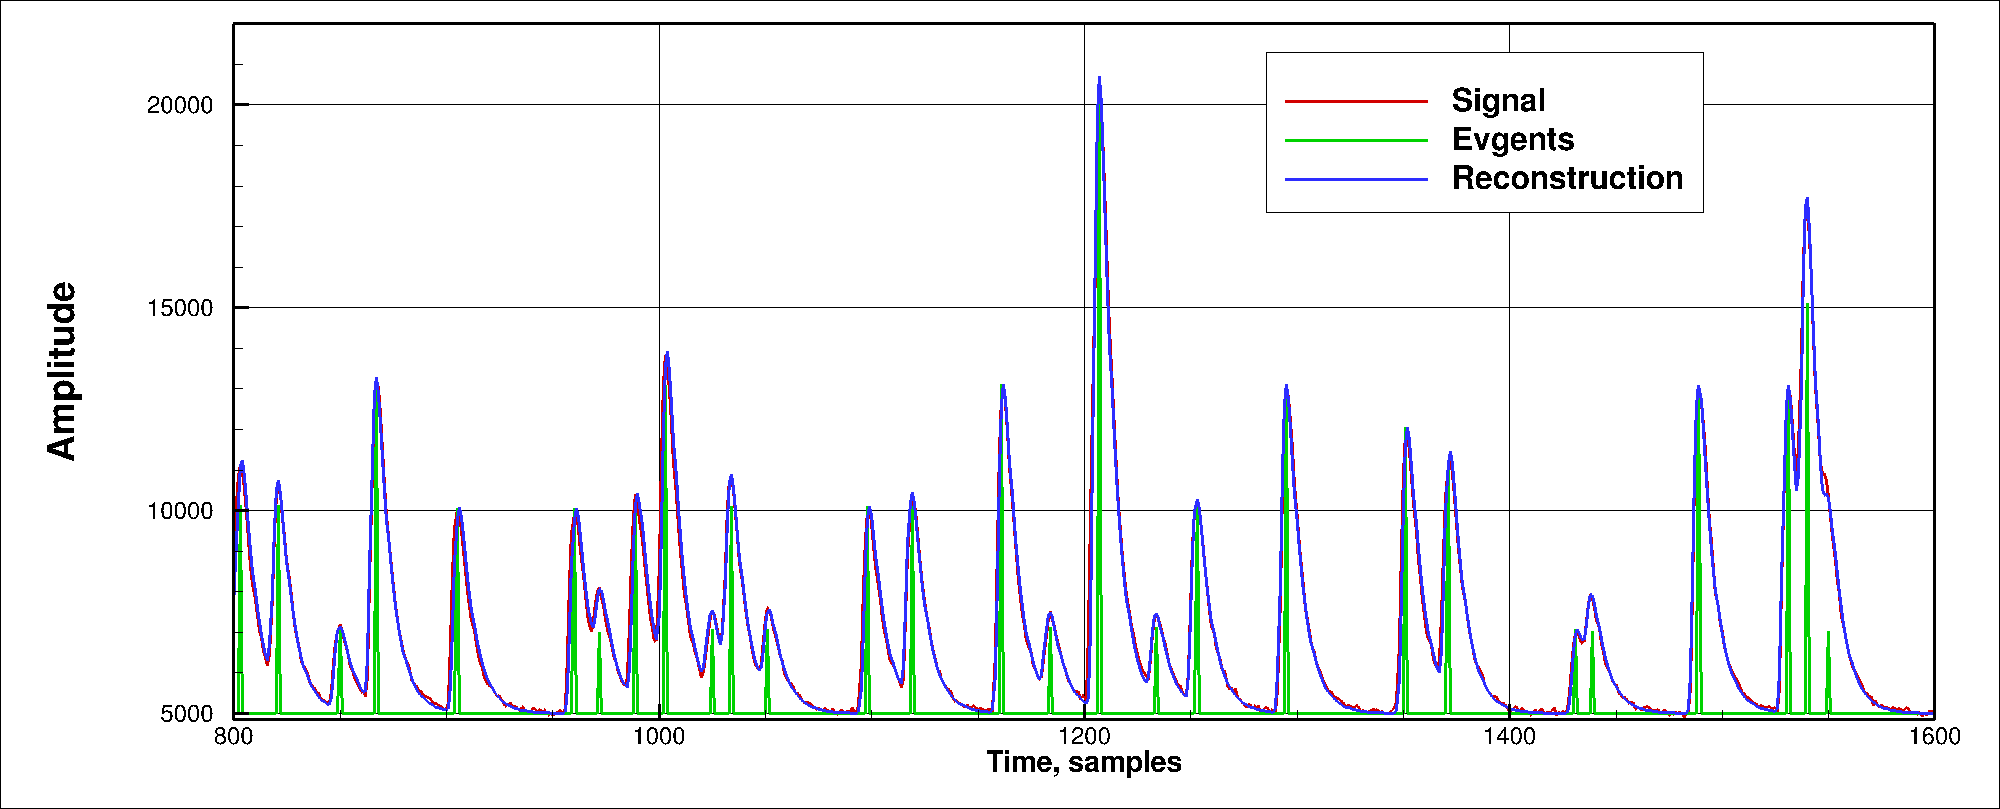
\includegraphics[width=0.95\linewidth]{fittingProcessing1e7} \\ а)
    \end{minipage}
    \vfill
    \begin{minipage}[b][][b]{0.95\linewidth}\centering
        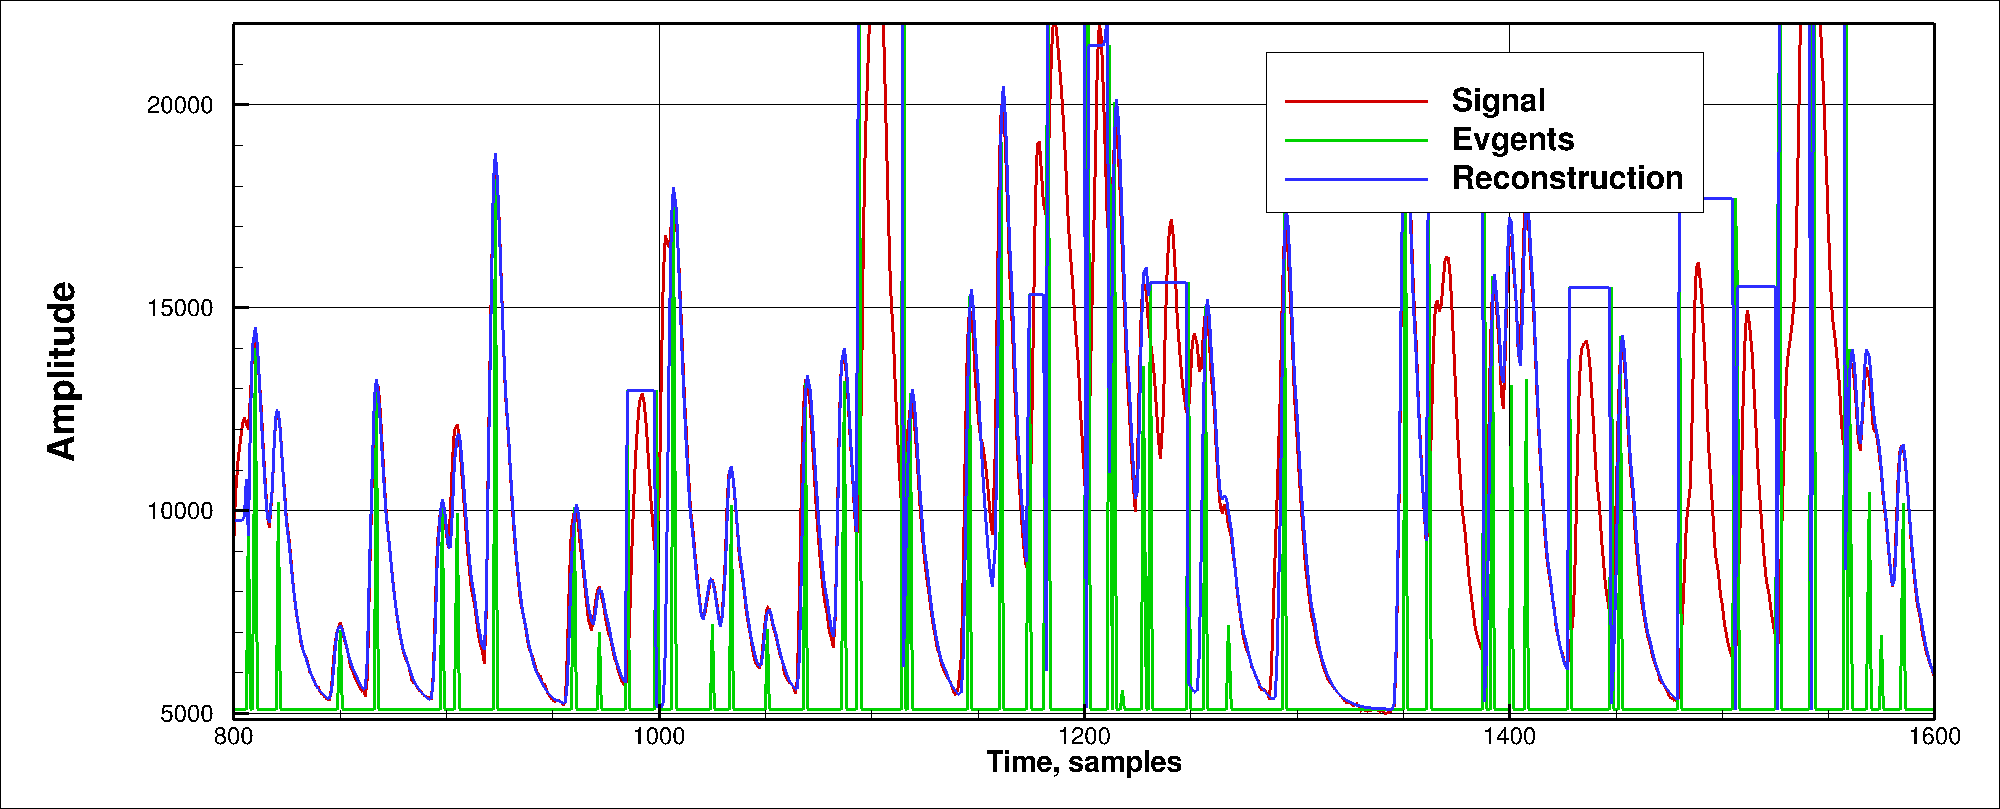
\includegraphics[width=0.95\linewidth]{fittingProcessing3e7} \\ б)
    \end{minipage}
    \vspace{5mm}
    \caption{ Пример работы алгоритма при обработке сигнала с загрузкой $10^7$~с${}^{-1}$~(а) и $3 \times 10^7$~с${}^{-1}$~(б). Красной линией обозначен модельный сигнал. Зелёным показан результат обработки сигнала с помощью алгоритма: импульсы, для которых $R/(E-B)<R^{max}$ и которые считаются успешно разобранными, представлены в виде единичных импульсов, а для импульсов, где $R/(E-B)>R^{max}$, на рисунке нарисован прямоугольник. Синим показан результат операции $z + \sum A_j p(t - t_j)$, то есть это такой сигнал, который соответствует разобранным импульсам; аналогично, для неразрешённых импульсов нарисован прямоугольник.~\cite{Khilkevitch2020}. }
    \label{fig:FittingProcessing}
\end{figure}

% ----------------------------------------------------------

\subsection{Деконволюция сигнала}

Методы деконволюции можно использовать для разделения сильно наложенных импульсов. Сигнал может быть представлен в виде свертки множества дельта-функций с ядром свертки, представляющим собой форму одиночного импульса: 
\begin{equation}
  \label{eq:SignalAsConvolution}
  s(t) = \int \limits_{-\infty}^{+\infty} p( t' - t ) \sum \limits_{i=0}{L} A_j \cdot \delta(t' - t_i) dt' + n(t)
\end{equation}
где $L$ --- количество гамма-событий. В дискретной форме, если пренебречь шумовой составляющей $n(t)$, это выражение приблизительно переписать как 
\begin{equation}
  s = P \cdot A
\end{equation}
где $s$ --- вектор отсчетов АЦП $s_i$, $P$ --- квадратная матрица свертки, $A$ --- вектор амплитуд импульсов. Значения матрицы $P$ равны
\begin{equation*}
  P_{i,j} = p( j - i )
\end{equation*}
Если время зарегистрированного события $t_j$ является целым числом, то значение вектора $A_{tj}$ равно значению амплитуды события. Если же вемя $t_j$ имеет дробную составляющую, то предполагается, что сумма двух соседних элементов вектора $A$ примерно равна амплитуде события $A_j$ при достаточно высокой частоте дискретизации АЦП по сравнению с длительностью импульса. Численный эксперимент показывает, что разница между суммой $A_{tj} + A_{tj+1}$ и истинной амплитудой $A_j$ не превышает 0.62\% для тестовой формы импульса.

Процедура деконволюции с использованием методов преобразования Фурье сложна из-за малой длительности импульса $p(t)$, часто около 20 отсчетов АЦП и менее, и желаемого дельта-образного решения~\cite{Morhac2011}. Можно использовать итерационные алгоритмы, такие как алгоритм Голда~\cite{Gold1964}. На каждой итерации этого алгоритма новое значение вычисляется как
\begin{equation*}
  A_i^k = \max \left( 0, \frac{A_i^{k-1} \cdot \widetilde{S_i} }{ \sum_{m=1}^{N} \widetilde{ P_{i,m} } \cdot A_m^{k-1} } \right)
\end{equation*}
где $k$ --- номер итерации, $\widetilde{S} = P^{T} \cdot S $, $\widetilde{P} = P^{T} \cdot P$, $N$ --- размер квадратной матрицы $P$ и вектора $A$.

В качестве начального условия можно выбирать значение сигналоа $A_i^0 = s_i$. Для обработки сигналов число итераций алгоритма можно сделать фиксированным, и равным некоторому значению, подбираемым опытным путем (например, 100~итераций). В процессе деконволюции для ускорения сходимости алгоритма через каждые несколько (например, 30) итераций можно проводить преобразование вида $A_i^k = \left( A_i^k \right)^g$, где значение степени $g$ --- параметр алгоритма, оно должно быть равным или чуть больше 1.0 (например, 1.05)~\cite{Morhac2011, Khilkevitch2020}.

На практике решение полного уравнения для всего сигнала целиком невозможно из-за чрезмерно большой размерности задачи, которая часто превышает $10^9$. Однако, поскольку функция отклика убывает, можно рассматривать за раз не весь сигнал целиком, а отдельные фрагменты сигнала, где его значение превышает порог $r$, и проводить деконволюцию только участков $\left[ B_j \ldots E_j \right] $. 

После деконволюции сигнала со значительным уровнем шума результатом является вектор $A$, в котором значения элементов часто не полностью соответствуют ожидаемым значениям: есть пики, не соответствующие никаким импульсам, которые возникли из-за шума исходного сигнала; но при этом одному реальному событию часто соответствует несколько соседних элементов вектора. Для получения амплитуд событий проводится суммирование групп соседних ненулевых значений вектора $A$. Все события меньше некоторого порога $r_A$ отбрасываются.

После вычисления амплитуд импульсов в интервале вычисляется невязка $R$. Если невязка больше определенного порогового значения $R^{max}$, то, как и в описанных выше алгортимах, можно считать что время и амплитуда событий на интервале были определены некорректно. В этом случае для коррекции спектра с учётом неразрешенных событий можно применить ту же процедуру, что и для методов фиттинга и суммирования.

Пример работы алгоритма показан на рисунке~\ref{fig:DeconvProcessing}.

\begin{figure}[ht]
    \begin{minipage}[b][][b]{0.95\linewidth}\centering
        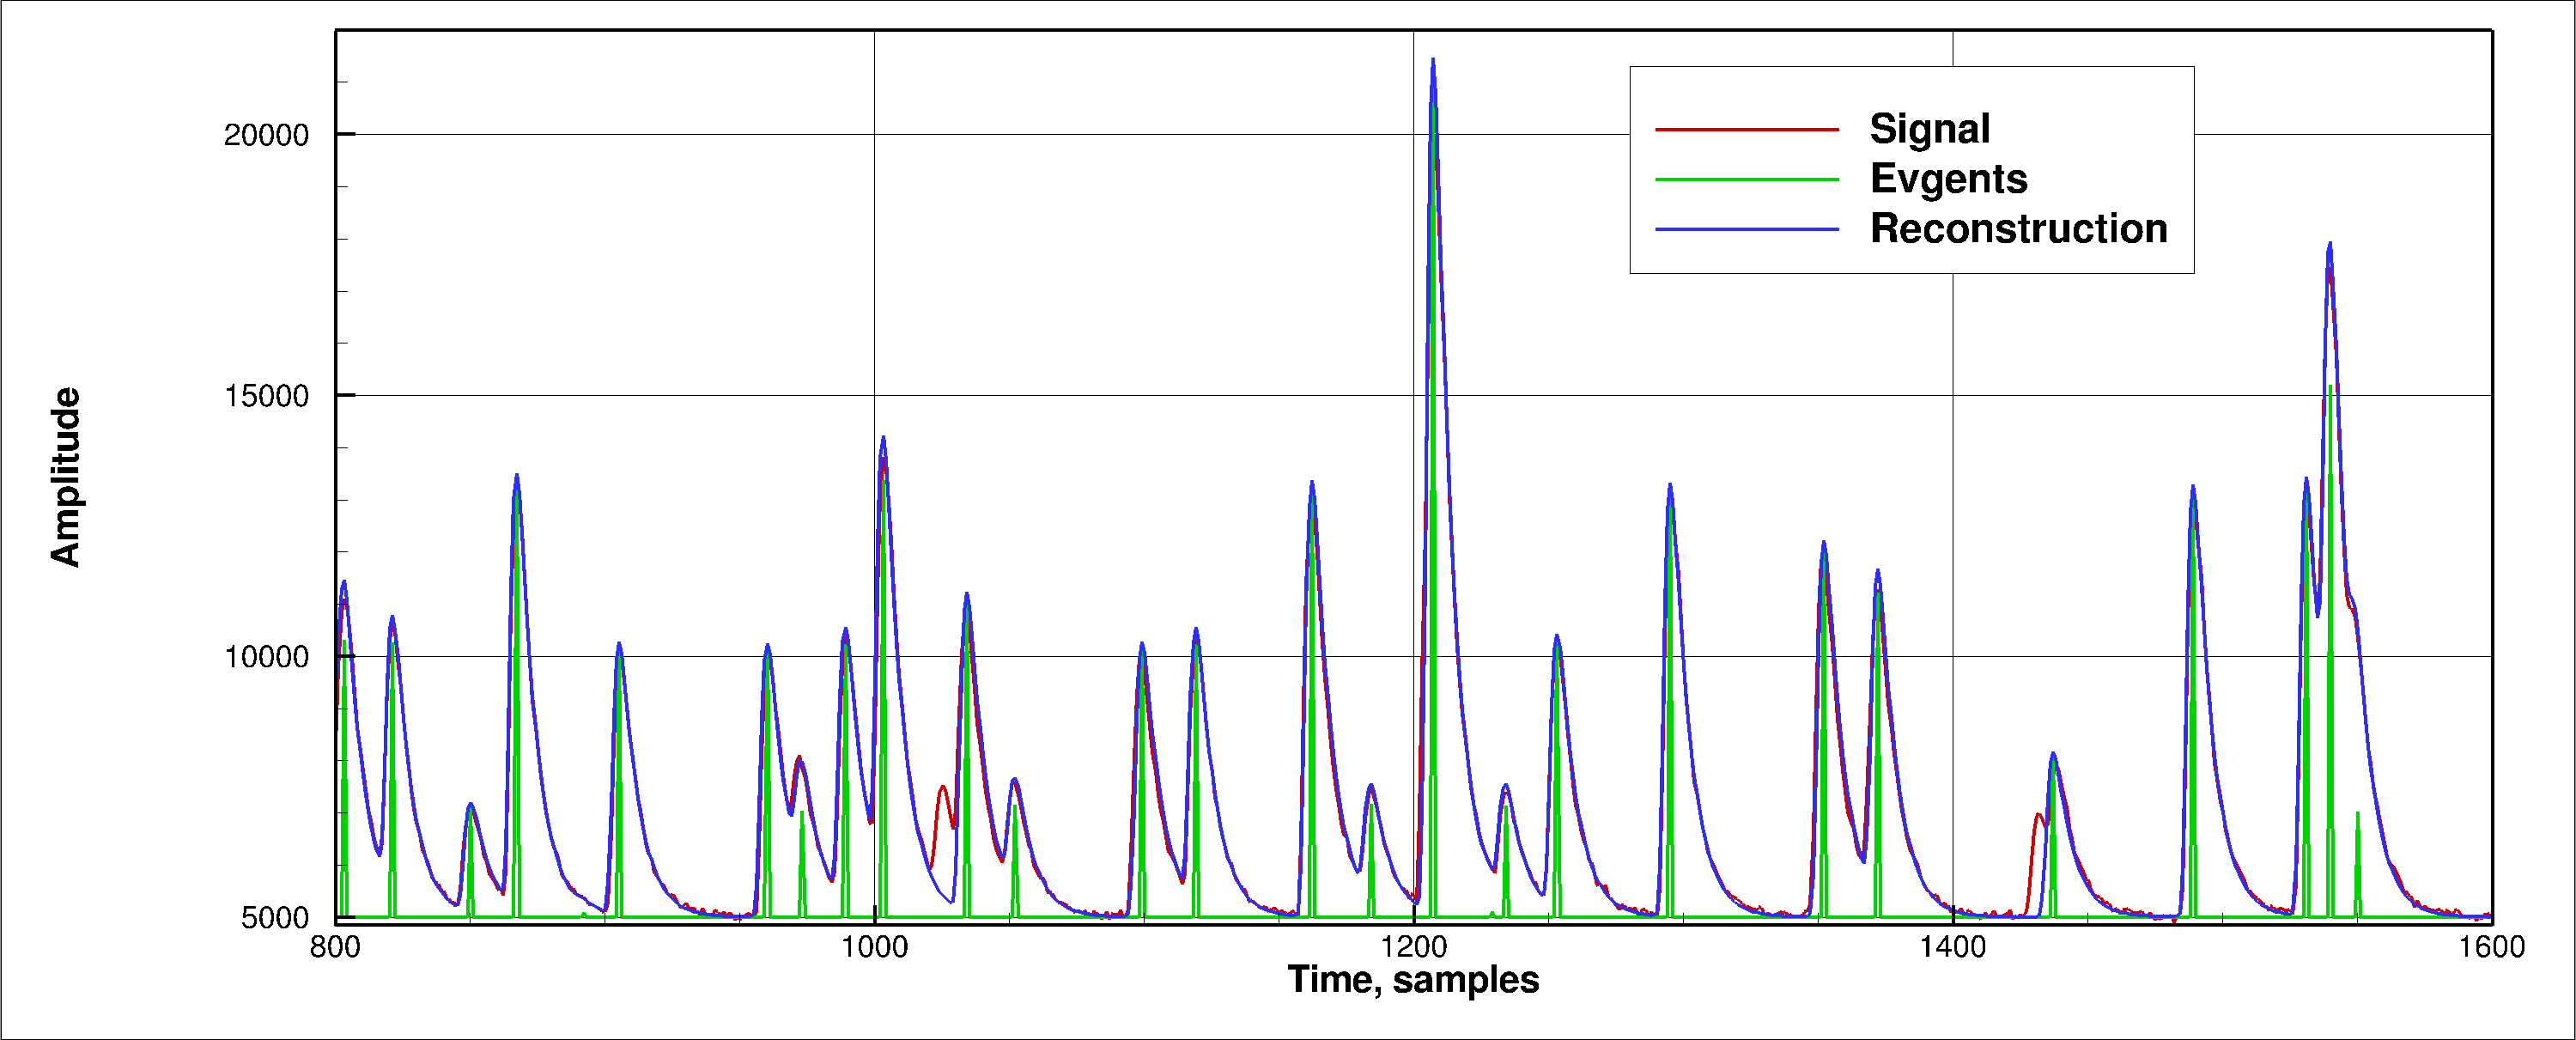
\includegraphics[width=0.95\linewidth]{deconvProcessing1e7} \\ а)
    \end{minipage}
    \vfill
    \begin{minipage}[b][][b]{0.95\linewidth}\centering
        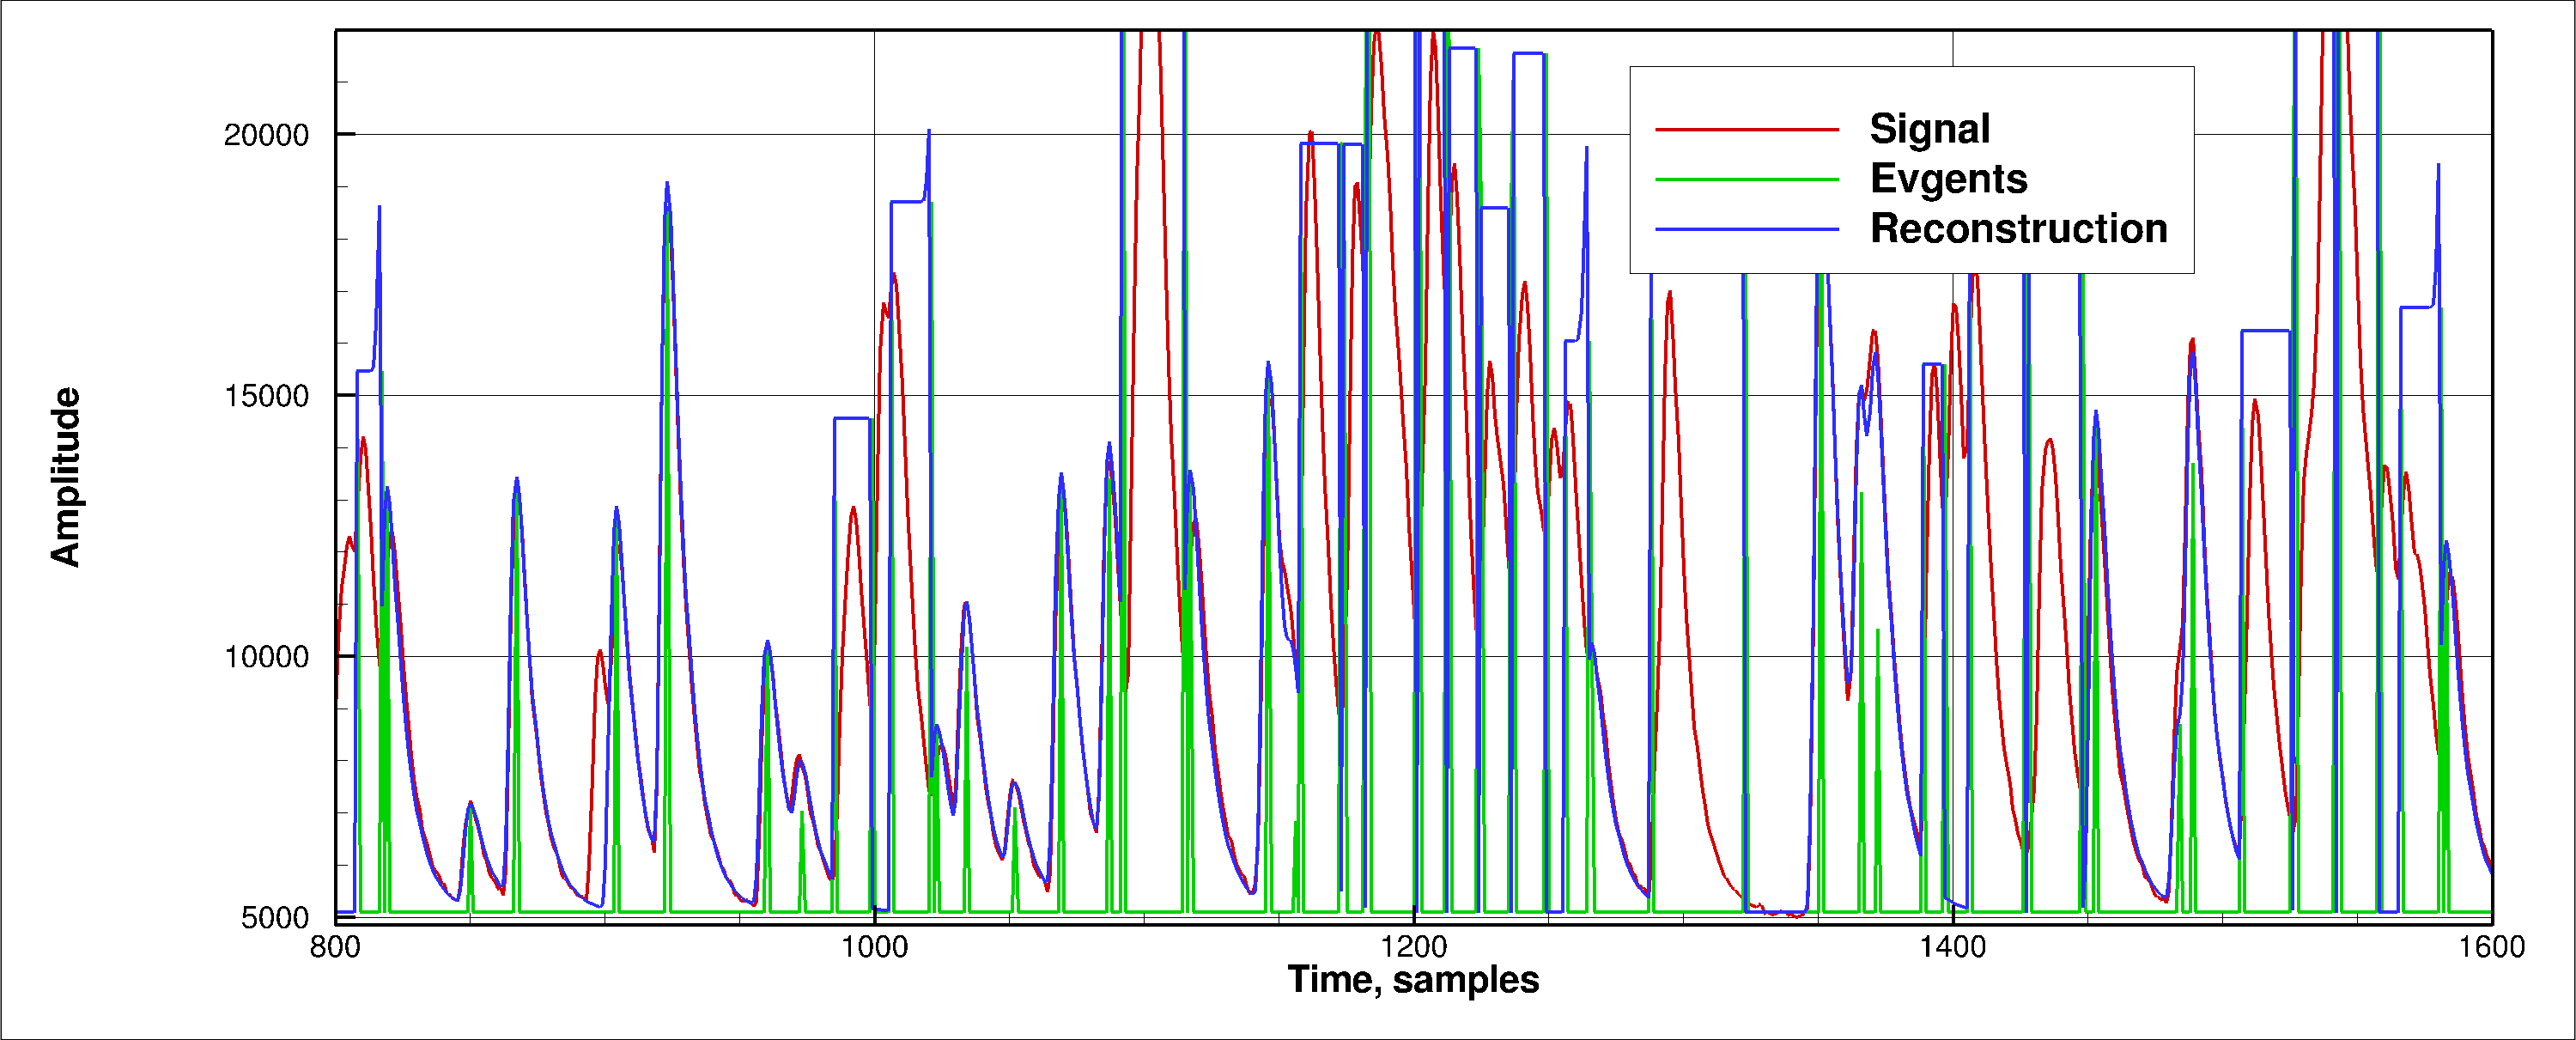
\includegraphics[width=0.95\linewidth]{deconvProcessing3e7} \\ б)
    \end{minipage}
    \vspace{5mm}
    \caption{ Пример работы алгоритма при обработке сигнала с загрузкой $10^7$~с${}^{-1}$~(а) и $3 \times 10^7$~с${}^{-1}$~(б). Красной линией обозначен модельный сигнал. Зелёным показан результат обработки сигнала с помощью алгоритма: импульсы, для которых $R/(E-B)<R^{max}$ и которые считаются успешно разобранными, представлены в виде единичных импульсов, а для импульсов, где $R/(E-B)>R^{max}$, на рисунке нарисован прямоугольник. Синим показан результат операции $z + \sum A_j p(t - t_j)$, то есть это такой сигнал, который соответствует разобранным импульсам; аналогично, для неразрешённых импульсов нарисован прямоугольник.~\cite{Khilkevitch2020}. }
    \label{fig:DeconvProcessing}
\end{figure}

% ----------------------------------------------------------

\subsection{Сравнение методов обрабоки сигнала}

Сравнение методов, описанных выше, для различных значений загрузки детектора, представлено на рисунках~\ref{fig:processingTotalCountRate},  \ref{fig:processingByWindowCountRate}, \ref{fig:processingByWindowFwhm}, \ref{fig:processingSpectrumCmpByMethods}, \ref{fig:processingSpectrumCmpByCountRate}. 

\begin{figure}[ht!]
  \centerfloat{ 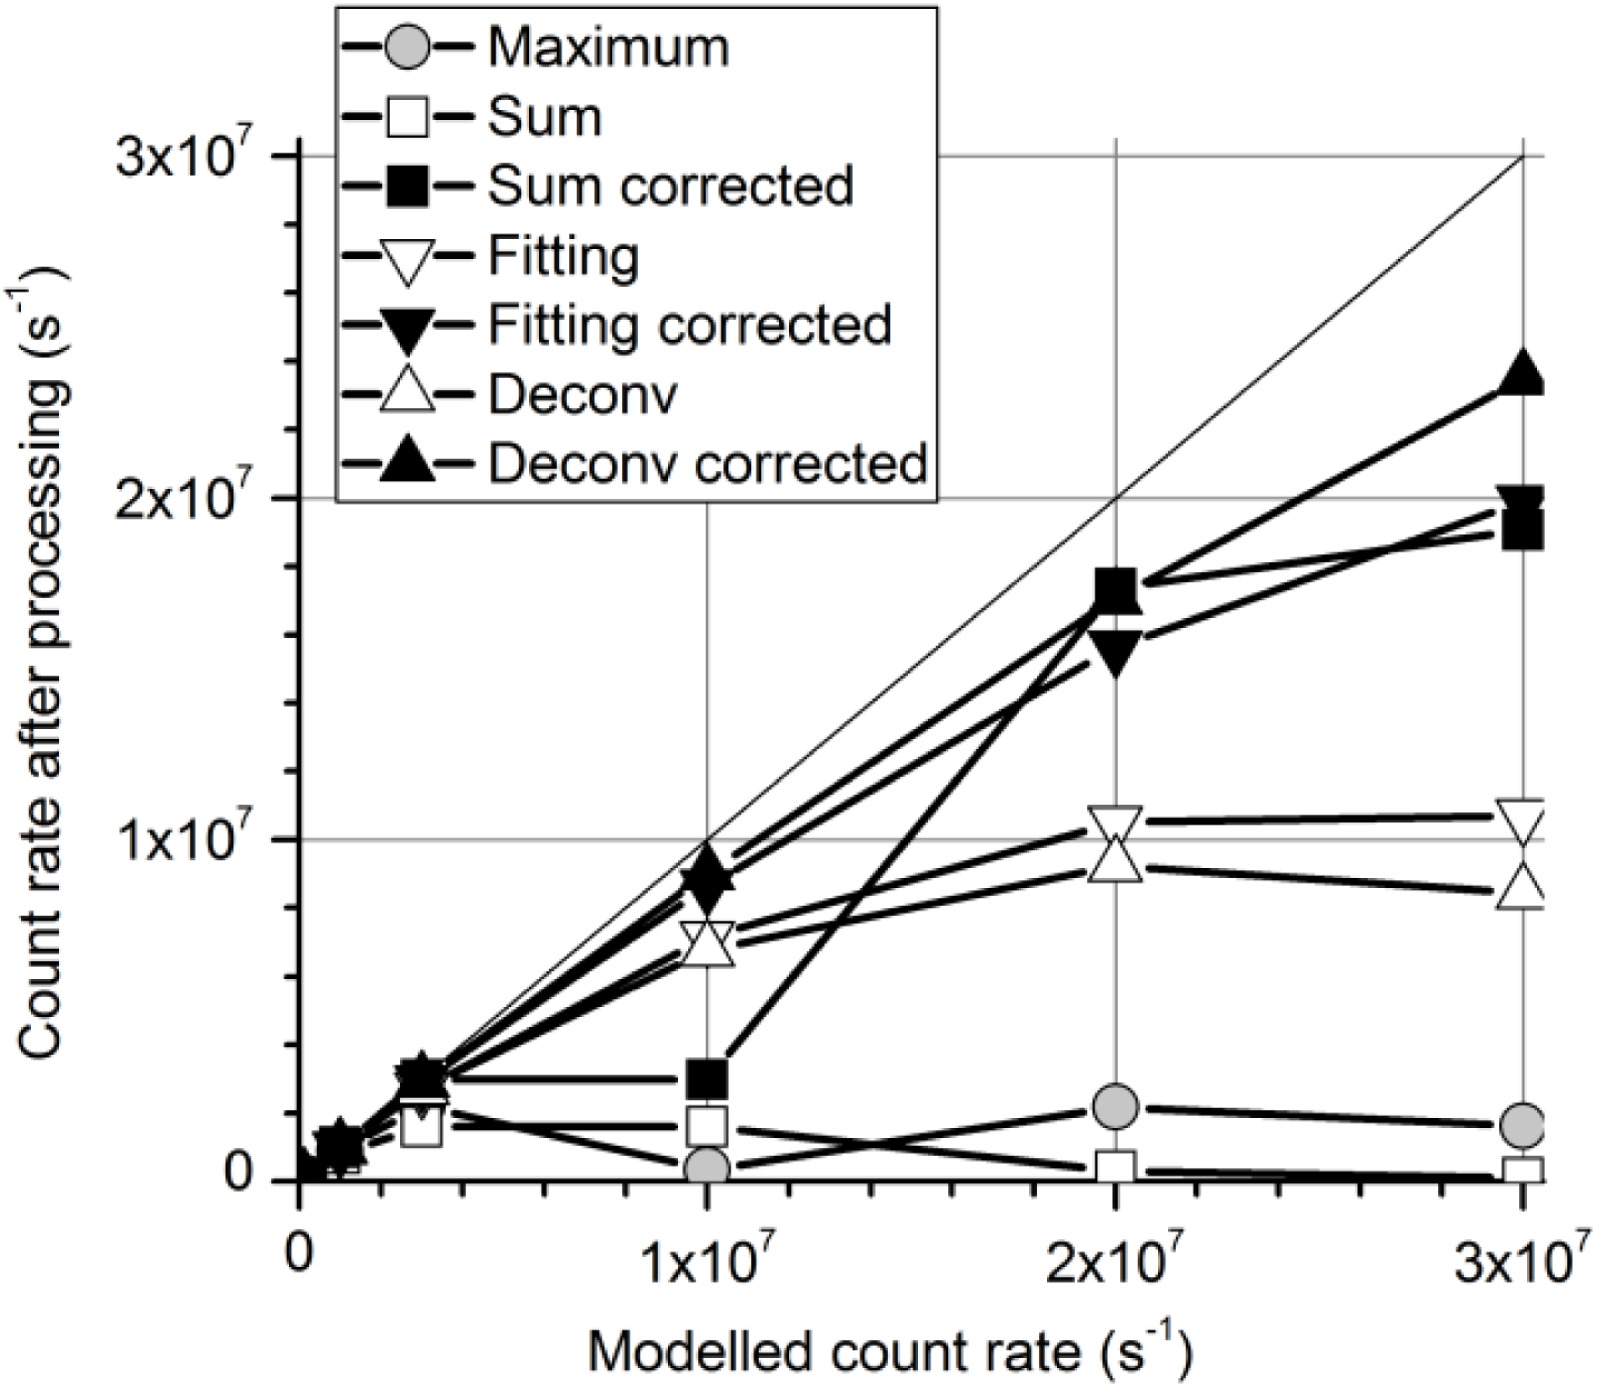
\includegraphics[width=0.60\linewidth]{processingTotalCountRate} }
  \caption{Общее количество зарегистрированных событий с энергиями выше 1~МэВ. В идеальном случае количество обнаруженных событий должно совпадать с количеством сгенерированных событий (сплошная линия). Однако из-за наложений во время обработки обнаруживается меньшее количество событий.~\cite{Khilkevitch2020} }
  \label{fig:processingTotalCountRate}
\end{figure}

\begin{figure}[ht!]
  \centerfloat{ 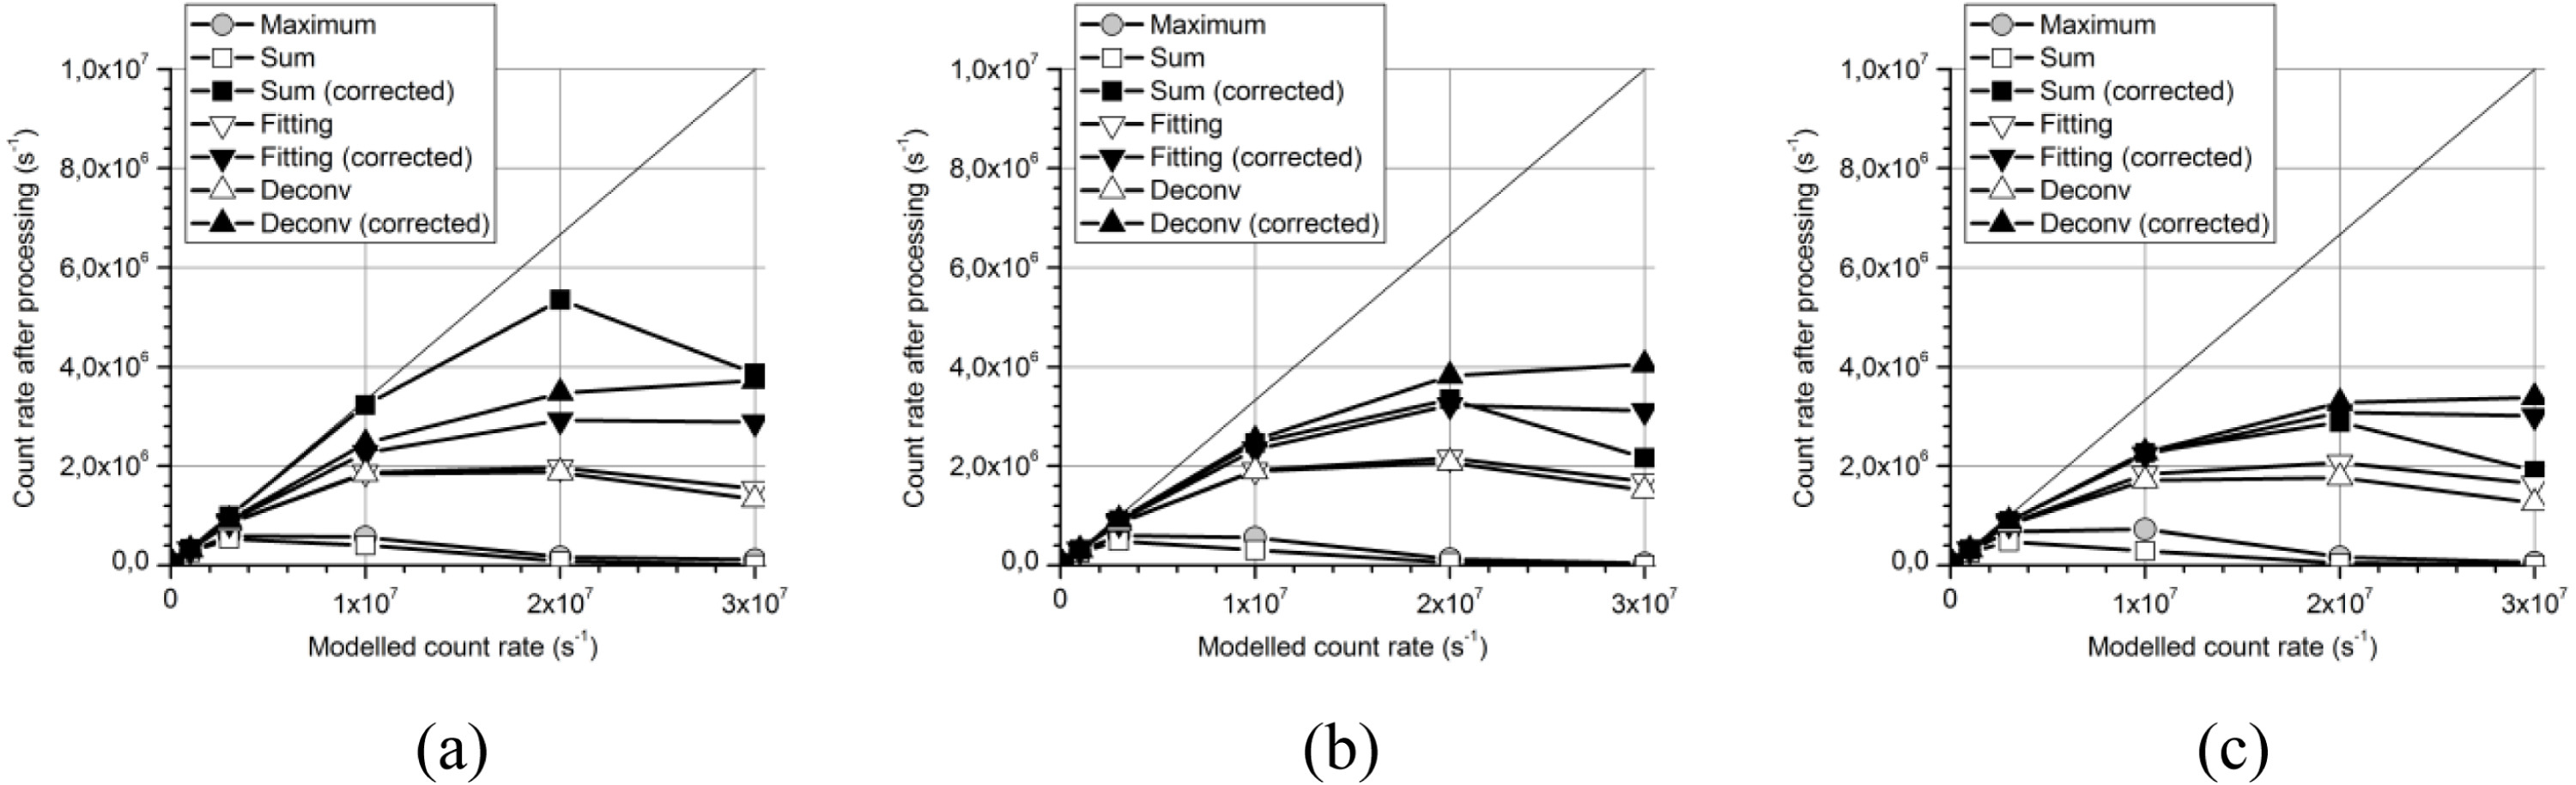
\includegraphics[width=0.95\linewidth]{processingByWindowCountRate} }
  \caption{ Количество событий в пиках с энергиями 2~МэВ~(а), 5~МэВ~(b) и 8~МэВ~(c) (в окне шириной 1~МэВ), полученных с использованием различных алгоритмов обработки. В идеальном случае количество обнаруженных событий должно быть равно одной трети количества сгенерированных событий (сплошные линии).~\cite{Khilkevitch2020} }
  \label{fig:processingByWindowCountRate}
\end{figure}

\begin{figure}[ht!]
  \centerfloat{ 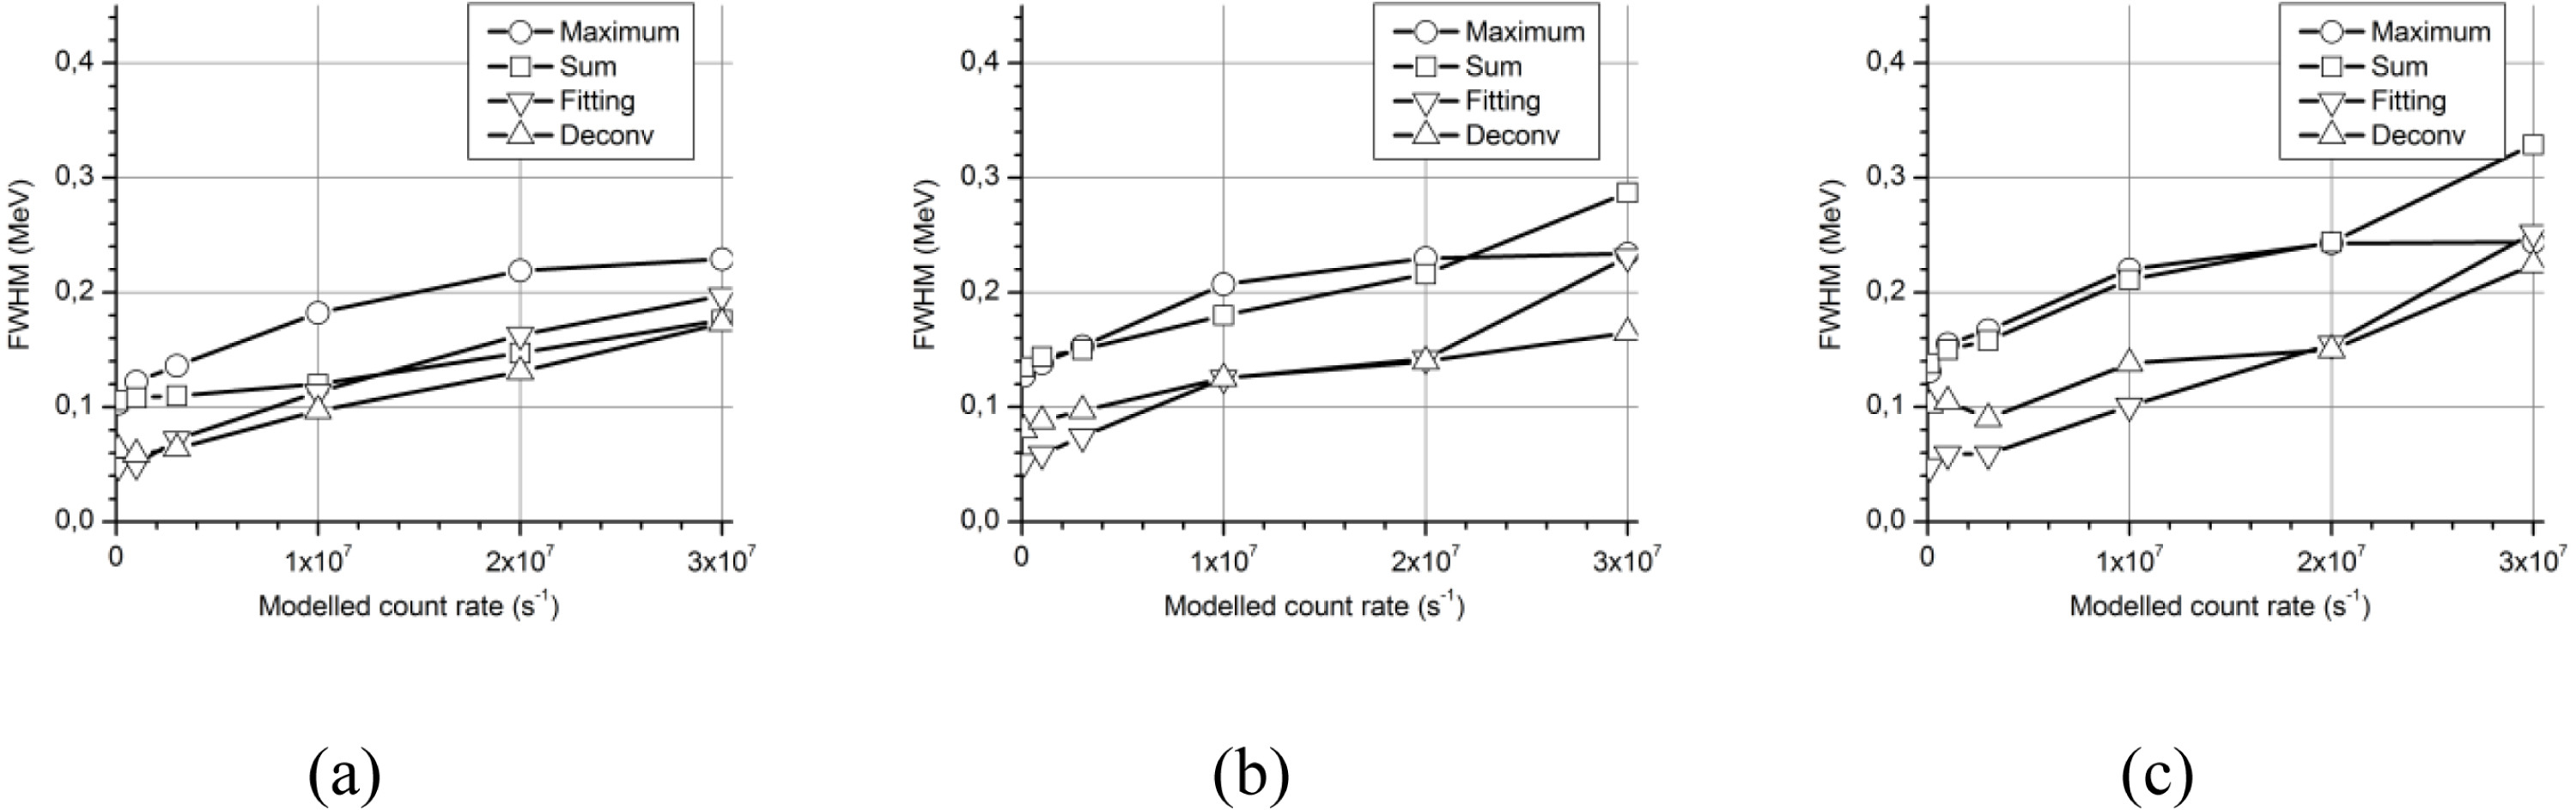
\includegraphics[width=0.95\linewidth]{processingByWindowFwhm} }
  \caption{ Полная ширина на полувысоте (FWHM) пиков при разных энергиях: 2~МэВ~(а), 5~МэВ~(b), 8~МэВ~(c).~\cite{Khilkevitch2020} }
  \label{fig:processingByWindowFwhm}
\end{figure}

\begin{figure}[ht!]
  \centerfloat{ 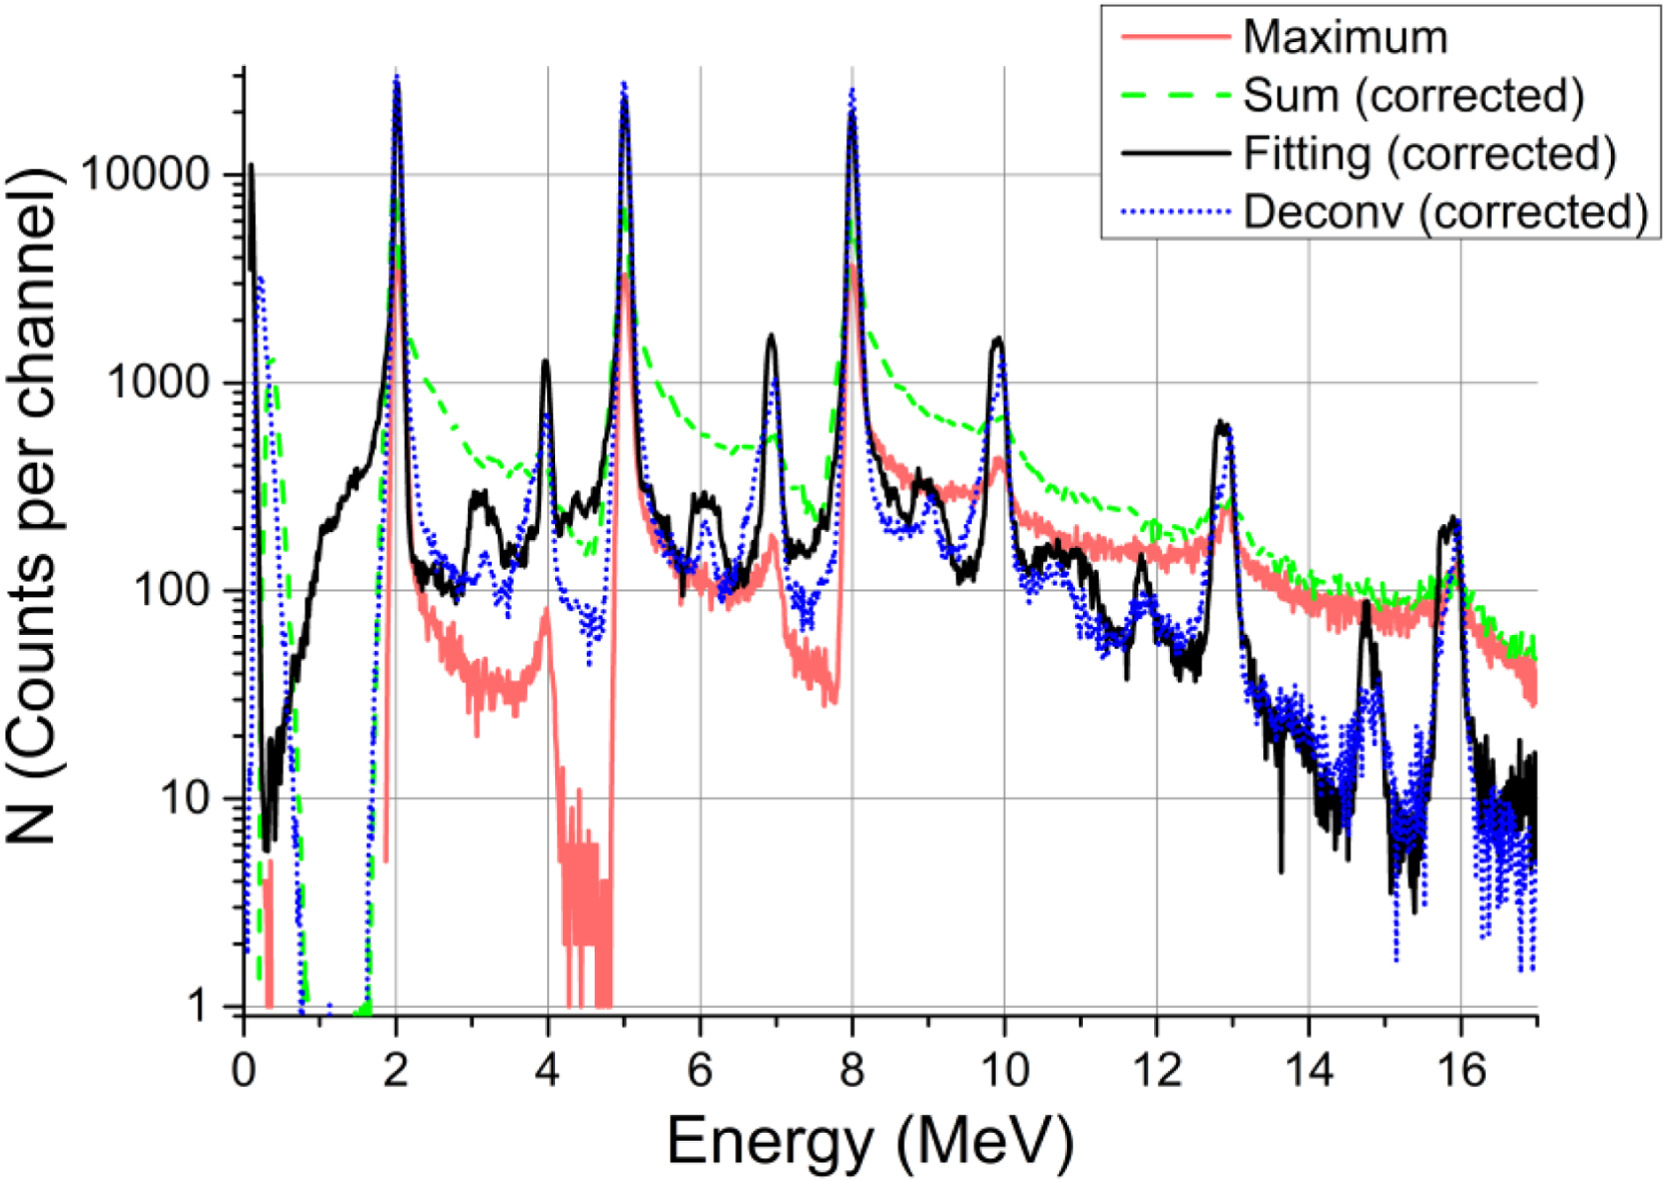
\includegraphics[width=0.60\linewidth]{processingSpectrumCmpByMethods} }
  \caption{ Спектры, полученные разными методами при загрузке детектора $10^7$~с${}^{-1}$. Спектры, полученные в ходе применения методов суммы, фиттигна и деконволюции показаны с коррекцией неразрешенных событий.~\cite{Khilkevitch2020} }
  \label{fig:processingSpectrumCmpByMethods}
\end{figure}

\begin{figure}[ht!]
  \centerfloat{ 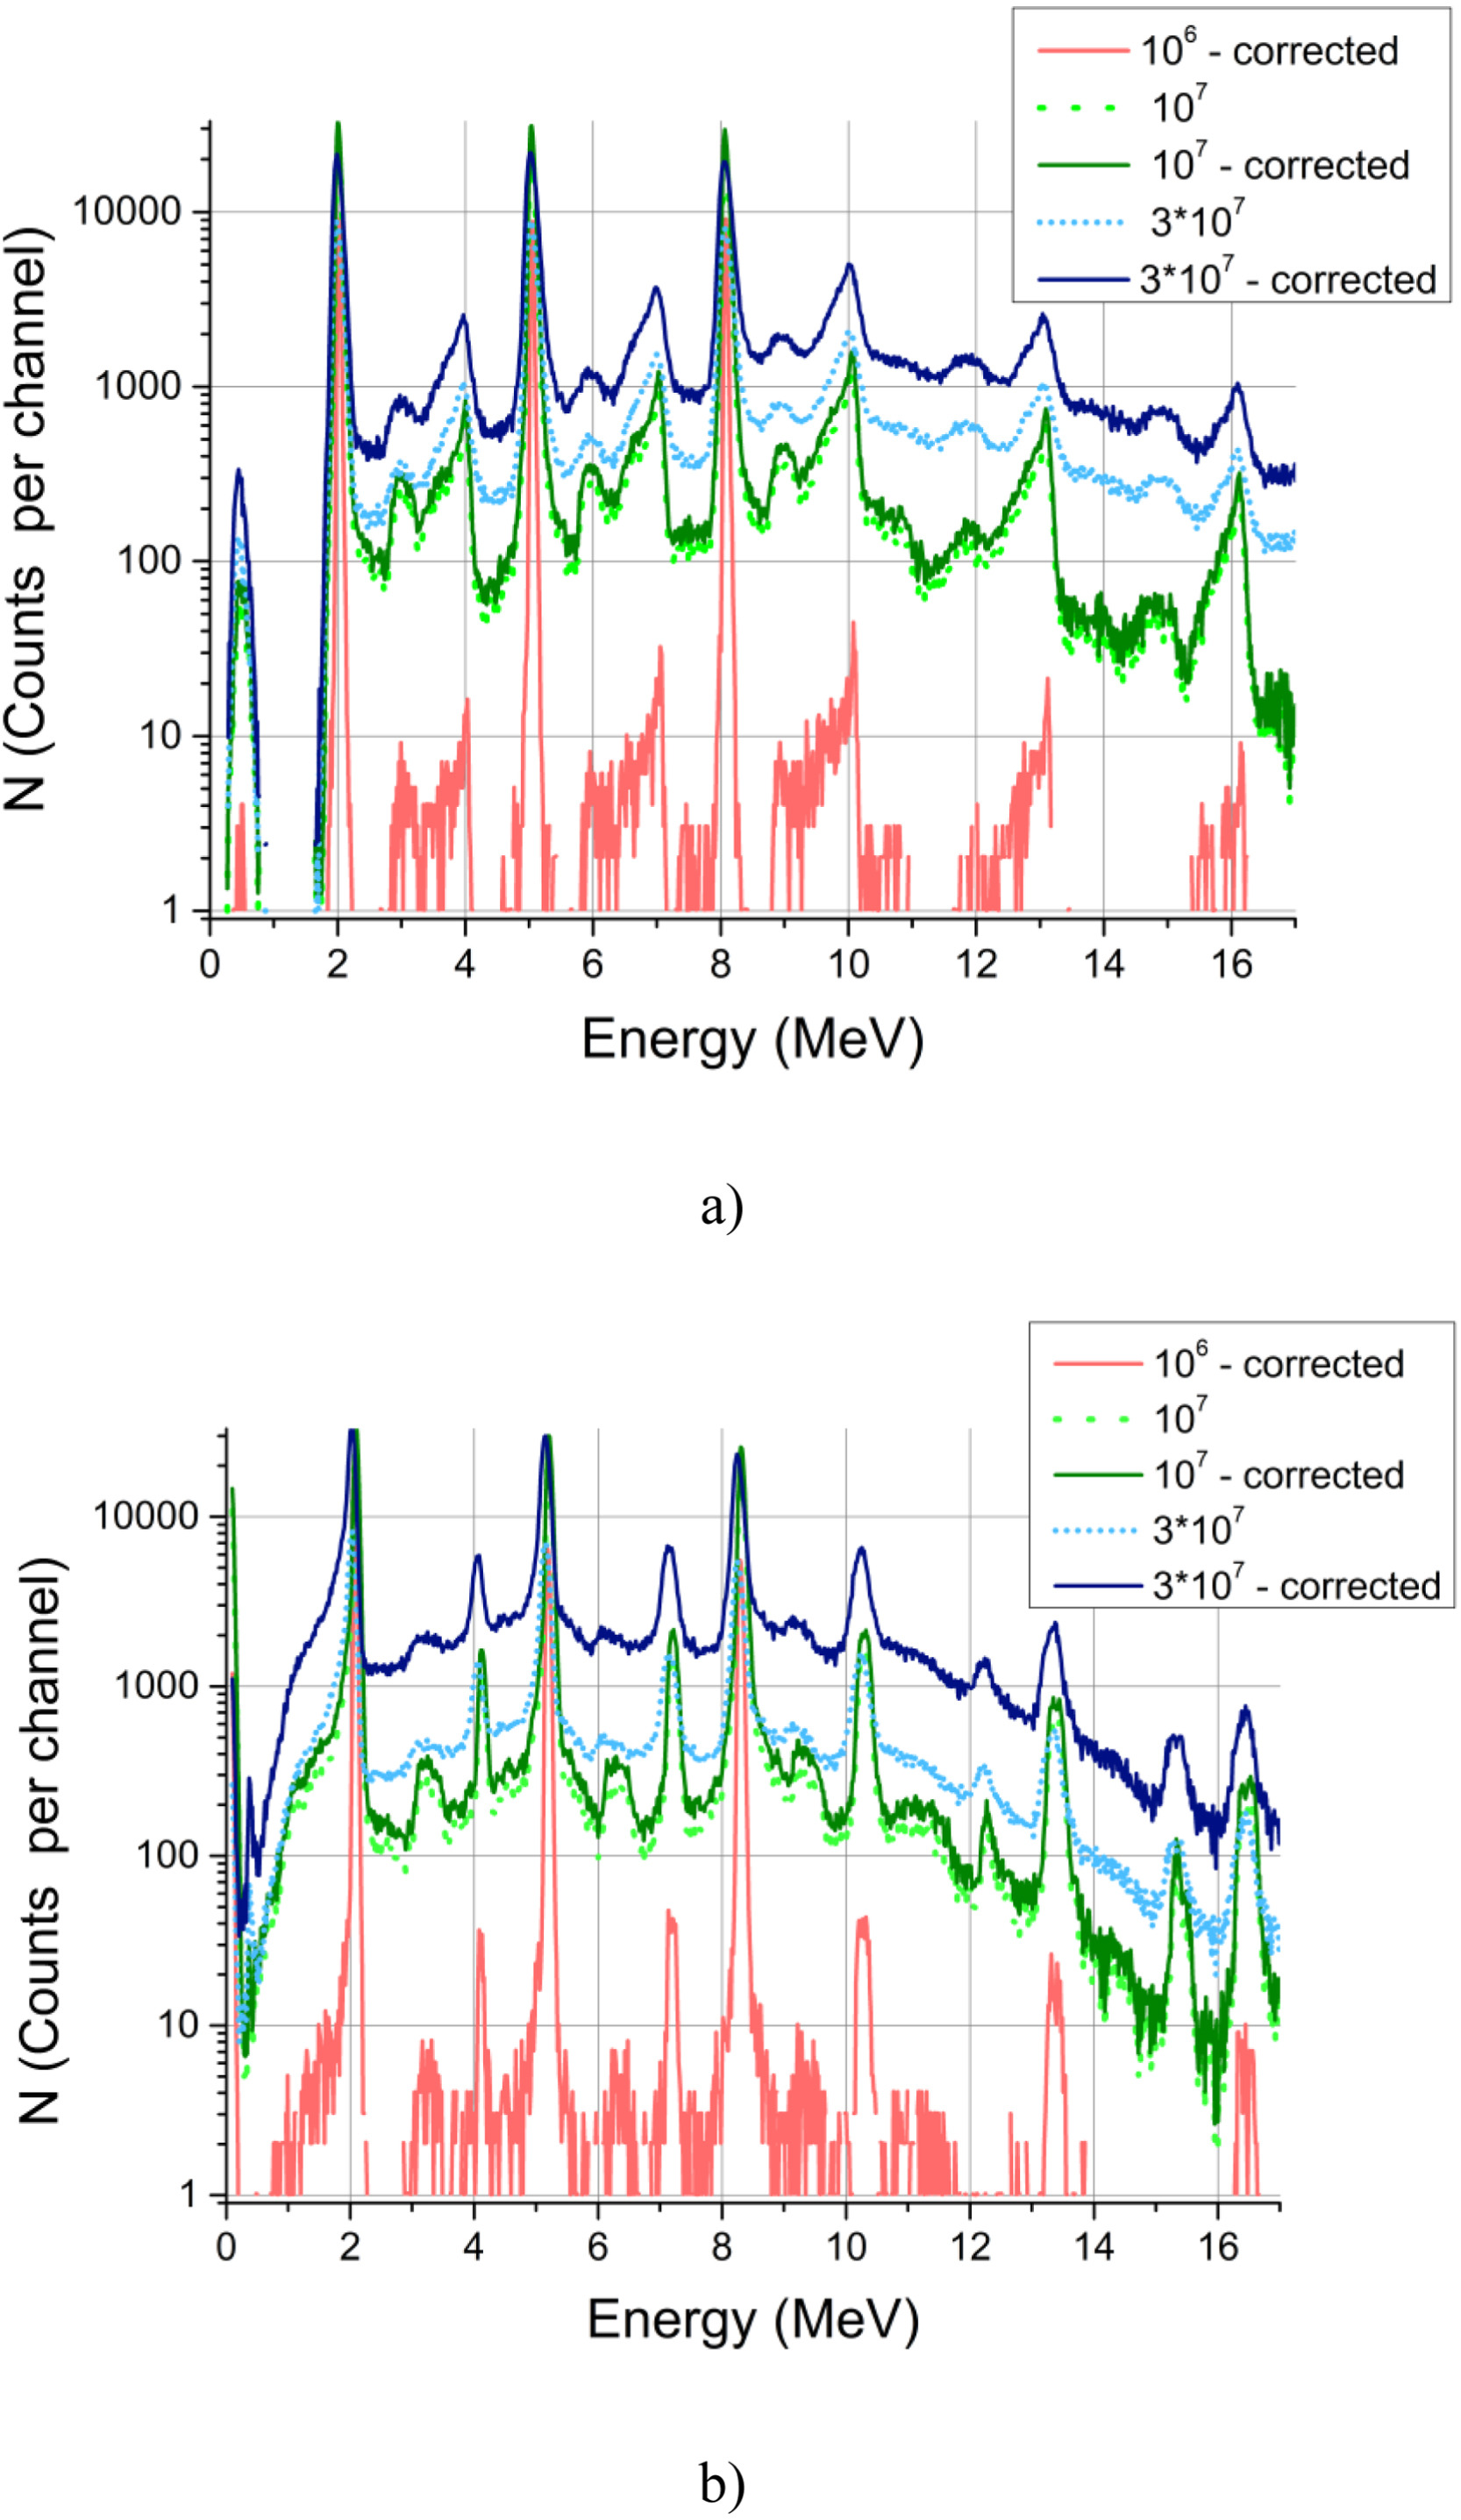
\includegraphics[width=0.60\linewidth]{processingSpectrumCmpByCountRate} }
  \caption{ Спектры, полученные методами фиттинга~(a) и деконволюции~(b). Линии, обозначенные как <<скорректированные>>, представляют собой спектры с коррекцией неразрешенных импульсов. При нагрузке $10^6$~с${}^{-1}$ спектры практически идентичны и их трудно различить на рисунках.~\cite{Khilkevitch2020} }
  \label{fig:processingSpectrumCmpByCountRate}
\end{figure}


Использованы модельные данные, созданные в разделе~\ref{sec:SignalGeneration}. На этих рисунках обозначения <<Sum corrected>>, <<Fitting corrected>> и <<Deconv corrected>> соответствуют данным, полученным с помощью алгоритмов <<суммы>>, <<фиттинга>> и <<деконволюции>> с учетом неразрешенных событий по ранее описанная процедуре. Эта поправка не влияет на форму результирующего спектра для стационарного источника излчения, как в модельном сигнале (однако, если спектр излучения меняется во времени, то это утверждение перестаёт быть верным). Однако такая коррекция позволяет получить более близкое к истинному количество событий, зарегистрированных детектором.

Использование метода <<максимум>> совершенно нецелесообразно при скоростях счета выше $3 \times 10^6$~с${}^{-1}$, так же как и использование метода <<суммы>> без коррекции неразрешённых событий из-за весьма высоких ошибок определения как общего числа событий, так и числа событий в одиночных пиках. Коррекция неразрешенных наложенных импульсов любым методом позволяет значительно улучшить результаты обработки сигнала. Наилучшие результаты определения числа импульсов в пиках дает метод деконволюции с коррекцией, дающий ошибку определения скорости счета при нагрузке $3 \times 10^7$~с${}^{-1}$ равной 21\%. Метод фиттинга с коррекцией менее точен, он дает погрешность скорости счета 33\% при той же нагрузке. Эта ошибка коррекции, по-видимому, увеличивается из-за роста количества слишком близких друг к другу импульсов, что приводит к тому, что они распознаются как одиночный импульс суммарной амплитуды. Метод суммы позволяет хорошо определить общее количество импульсов после коррекции, но количество неразрешенных событий при использовании этого алгоритма чрезвычайно велико при высоких нагрузках, что затрудняет его использование при измерении гамма-излучения высокотемпературной плазмы токамака, в котором спектр может значительно изменяться за короткие промежутки времени.

При определении интенсивностей отдельных пиков картина меняется. Погрешность определения интенсивности одиночных пиков при нагрузке свыше $10^7$~с${}^{-1}$ быстро возрастает. Это можно объяснить тем, что, хотя методы позволяют разделить наложенные импульсы, ошибки в определении их амплитуды становятся очень значительными для всех алгоритмов.

На рисунке~\ref{fig:processingByWindowFwhm} показано разрешение (полная ширина на полувысоте, FWHM) пиков с энергиями 2~МэВ, 5~МэВ и 8~МэВ с при обработке сигнала различными алгоритмами. Алгоритмы фиттинга и деконволюции позволяют получить разрешение отдельных пиков намного лучше, чем алгоритмы максимума и суммы. Алгоритм деконволюции несколько лучше алгоритма фиттинга при высоких значениях нагрузки ($2 \times 10^7$~с${}^{-1}$ и выше) и немного хуже при низких значениях нагрузки. По-видимому, это связано с тем, что данный алгоритм вносит дополнительную погрешность при учете событий, время регистрации которых находится между соседними отсчетами АЦП. Однако этот алгоритм позволяет лучше разделять очень близко наложенные друг на друга события, что важно при высокой загрузке детектора. При высоких нагрузках  алгоритм <<по максимуму>> имеет разрешение, сравнимое с более сложными алгоритмами; однако, принимая во внимание тот факт, что при такой нагрузке он позволяет регистрировать лишь около 5\% всех событий, трудно говорить о его применимости для таких нагрузок детекторов.

Спектры, построенные с использованием различных методов определения амплитуды импульса, представлены на рисунках~\ref{fig:processingSpectrumCmpByMethods} и \ref{fig:processingSpectrumCmpByCountRate}. На спектрах различимы пики с энергиями 4~МэВ, 7~МэВ и 10~МэВ, тогда как в исходном сигнале были сгенерированы только пики с энергиями 2~МэВ~, 5~МэВ, 8~МэВ. Пики появляются из-за очень близко наложенных событий, которые не могут быть разрешены с помощью алгоритмов. Такие пики практически неотличимы от единичного события с амплитудой, равной сумме этих событий. Видны пики с энергией 4~МэВ (сумма двух событий с энергией 2~МэВ), 7~МэВ (сумма двух событий с энергией 2~МэВ и 5~МэВ), 10~МэВ (сумма двух событий с энергией 5~МэВ или с энергиями 2~МэВ и 8~МэВ), 13~МэВ (сумма двух событий с энергиями 5~МэВ и 8~МэВ).

Форма и амплитуда пиков, полученные методами максимума и суммы, сильно искажаются даже при нагрузке $10^7$~с${}^{-1}$. Форма пиков в спектрах, построенных с помощью методов фиттинга и деконволюции, остаётся симметричной даже при загрузках до $3 \times 10^7$~с${}^{-1}$. Для такой загрузке метод деконволюции сохранил симметрию формы и для пиков, являющихся суммами событий. В стационарном источнике спектры с коррекцией отличаются от спектров без нее лишь постоянным множителем~\cite{Khilkevitch2020}.

% ----------------------------------------------------------

\subsection{Влияние шума на результаты обработки}

Для демонстрации влияния шума на результаты различных алгоритмов был сгенерирован дополнительный набор модельных сигналов с нагрузкой $10^7$~с${}^{-1}$ и различными значениями уровня шума $\sigma_n$ в диапазоне от 10 до 500. Остальные параметры сигнала такие же, как описано в разделе~\ref{sec:SignalGeneration}, включая калибровку. Эти тестовые сигналы обрабатывались с использованием различных алгоритмов. Влияние шума на результаты алгоритмов иллюстрируют рисунки~\ref{fig:processingNoiceByWindowCountRate}, \ref{fig:processingNoiceByWindowFwhm}, \ref{fig:processingSpectrumCmpByNoice}.

\begin{figure}[ht!]
  \centerfloat{ 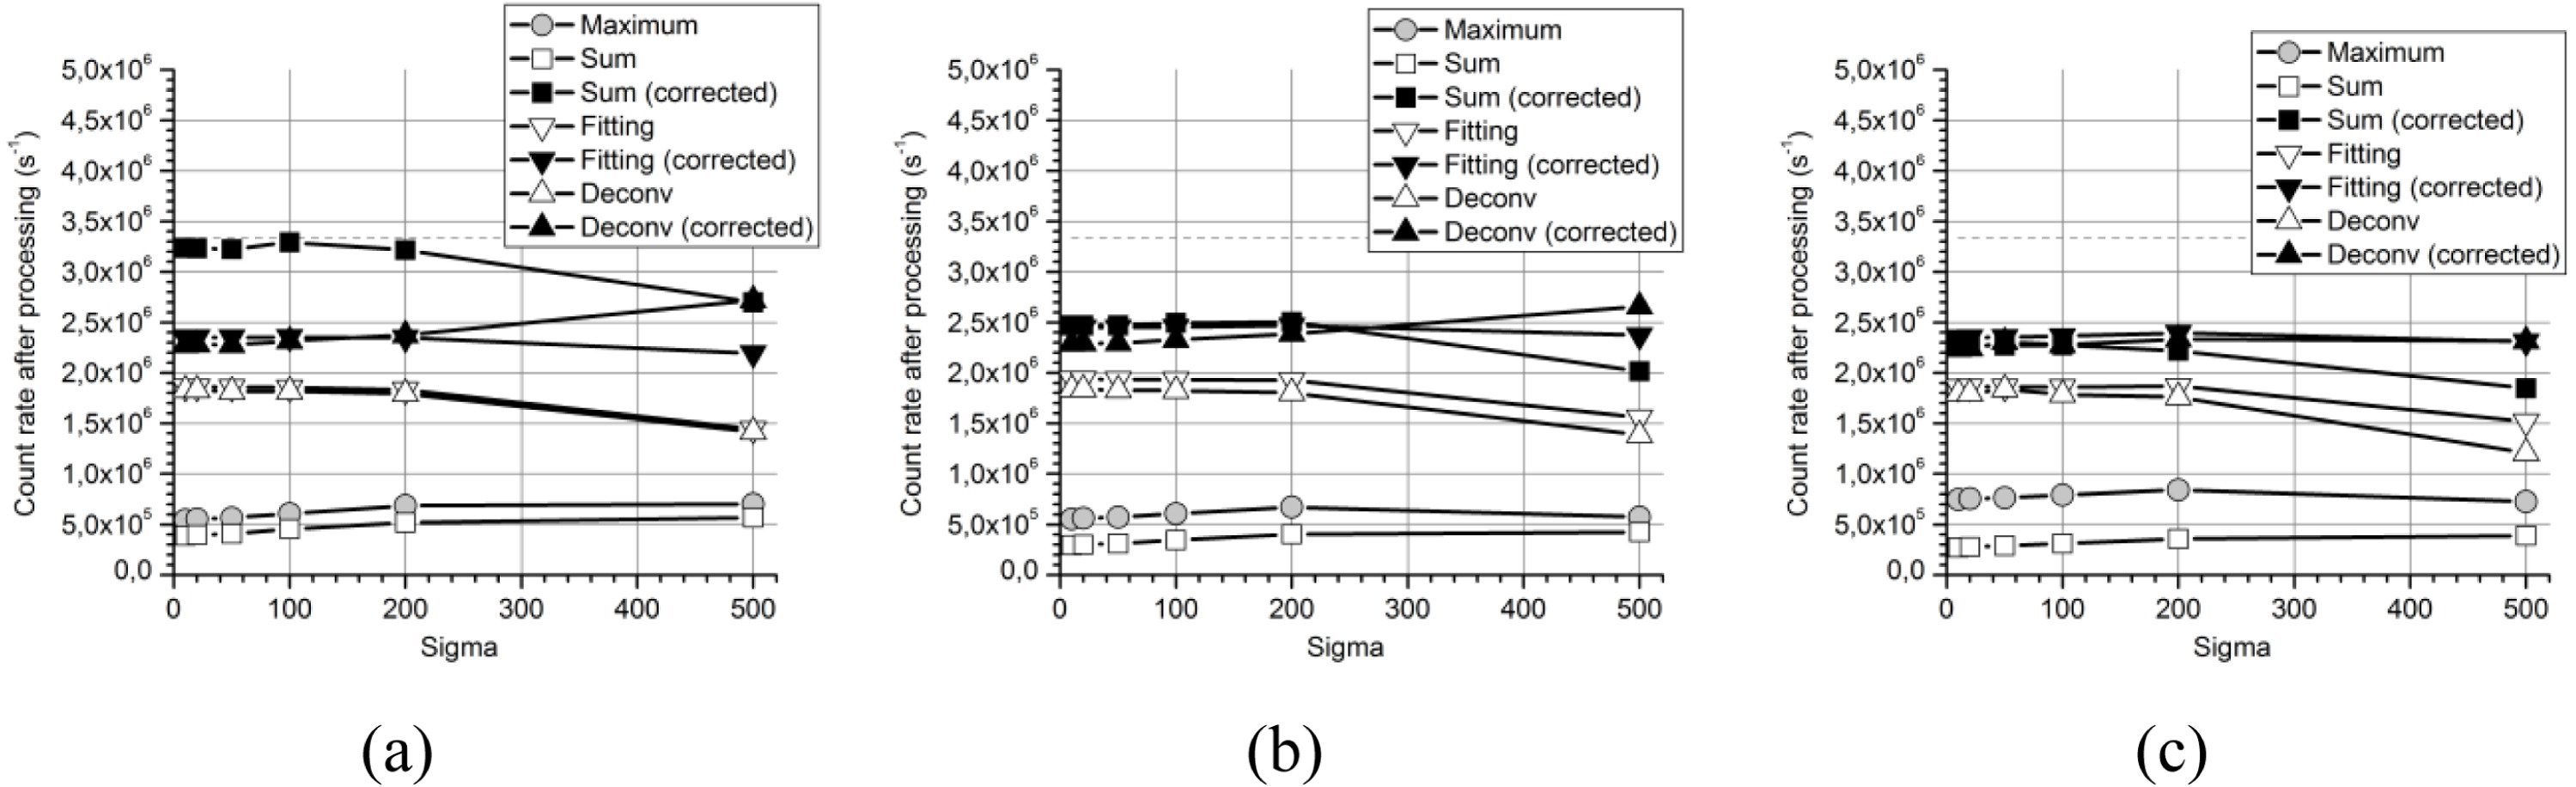
\includegraphics[width=0.95\linewidth]{processingNoiceByWindowCountRate} }
  \caption{ Количество событий в пиках с энергиями: 2~МэВ~(a), 5~МэВ~(b) и 8~МэВ~(c) (в окне шириной 1~МэВ), полученных с использованием различных алгоритмов обработки при разных значениях $\sigma_n$. Количество событий в идеальном случае равно $3.33 \times 10^6$.~\cite{Khilkevitch2020} }
  \label{fig:processingNoiceByWindowCountRate}
\end{figure}


\begin{figure}[ht!]
  \centerfloat{ 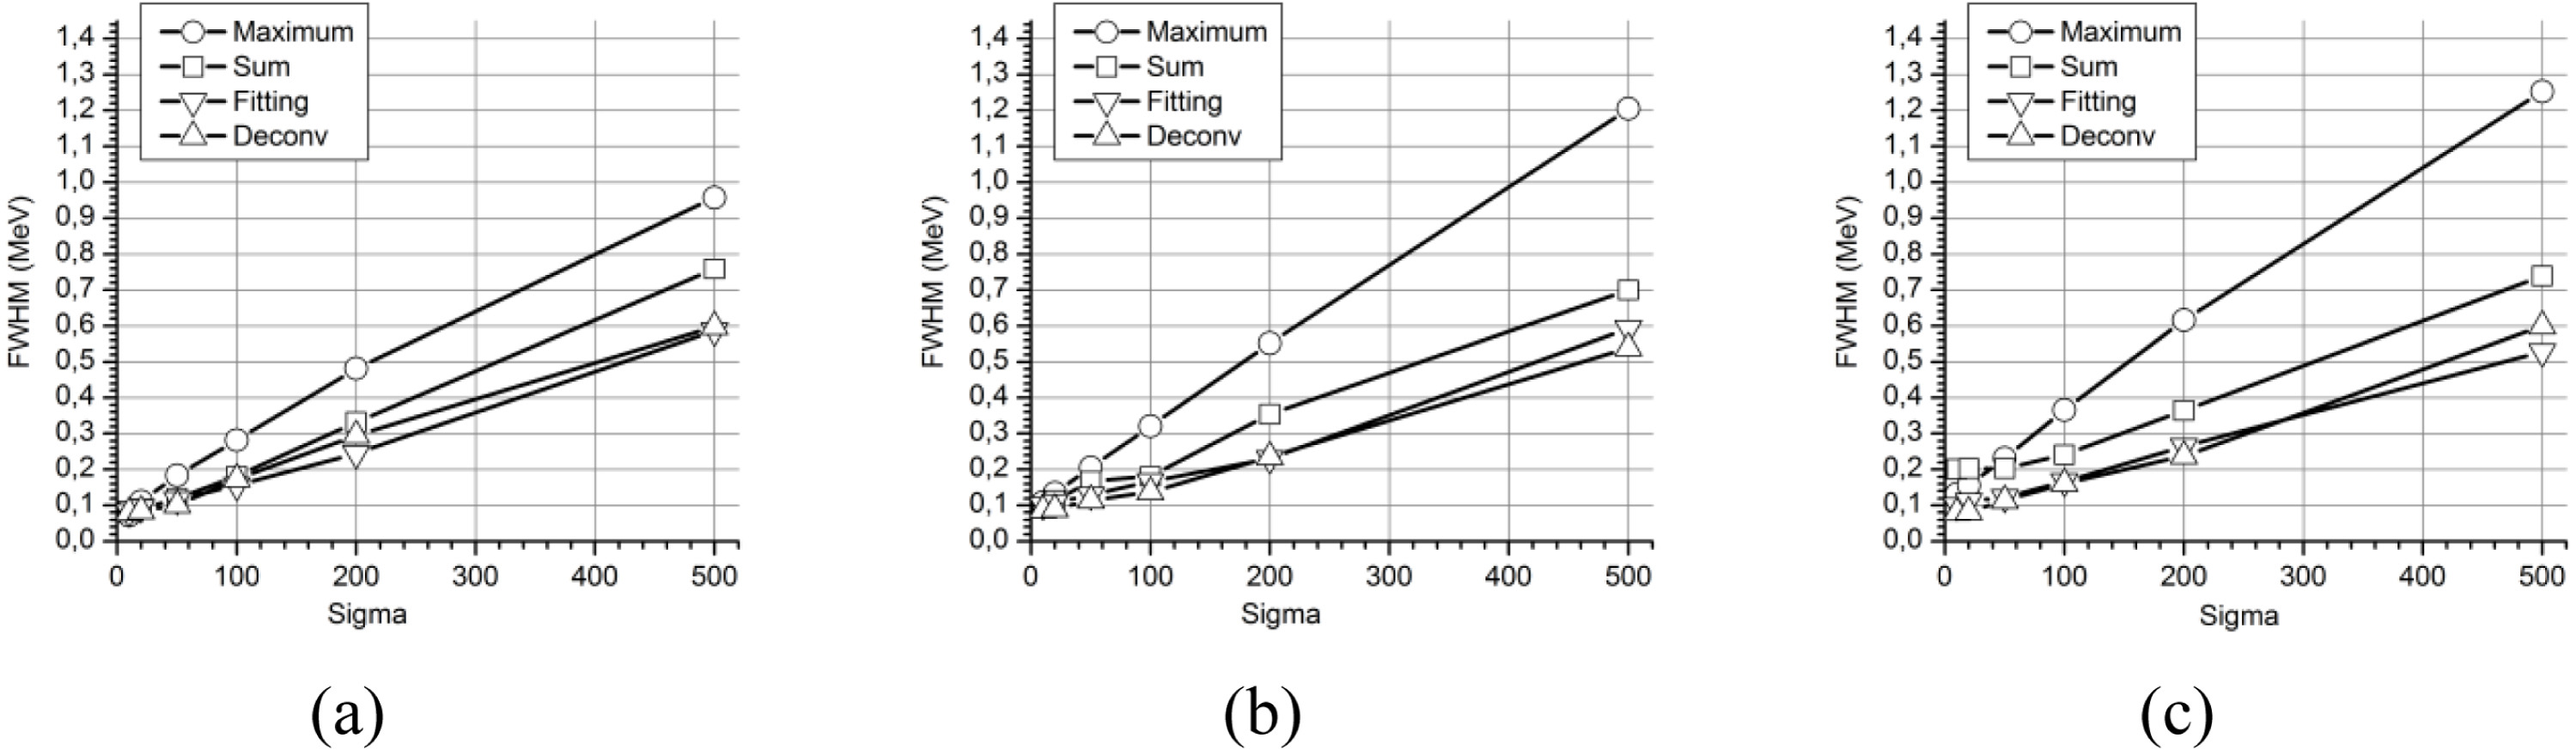
\includegraphics[width=0.95\linewidth]{processingNoiceByWindowFwhm} }
  \caption{ Полная ширина на полувысоте (FWHM) для пиков с энергиями: 2~МэВ~(a), 5~МэВ~(b) и 8~МэВ~(c), полученные с использованием различных алгоритмов обработки при разных значениях $\sigma_n$.~\cite{Khilkevitch2020} }
  \label{fig:processingNoiceByWindowFwhm}
\end{figure}

\begin{figure}[ht!]
  \centerfloat{ 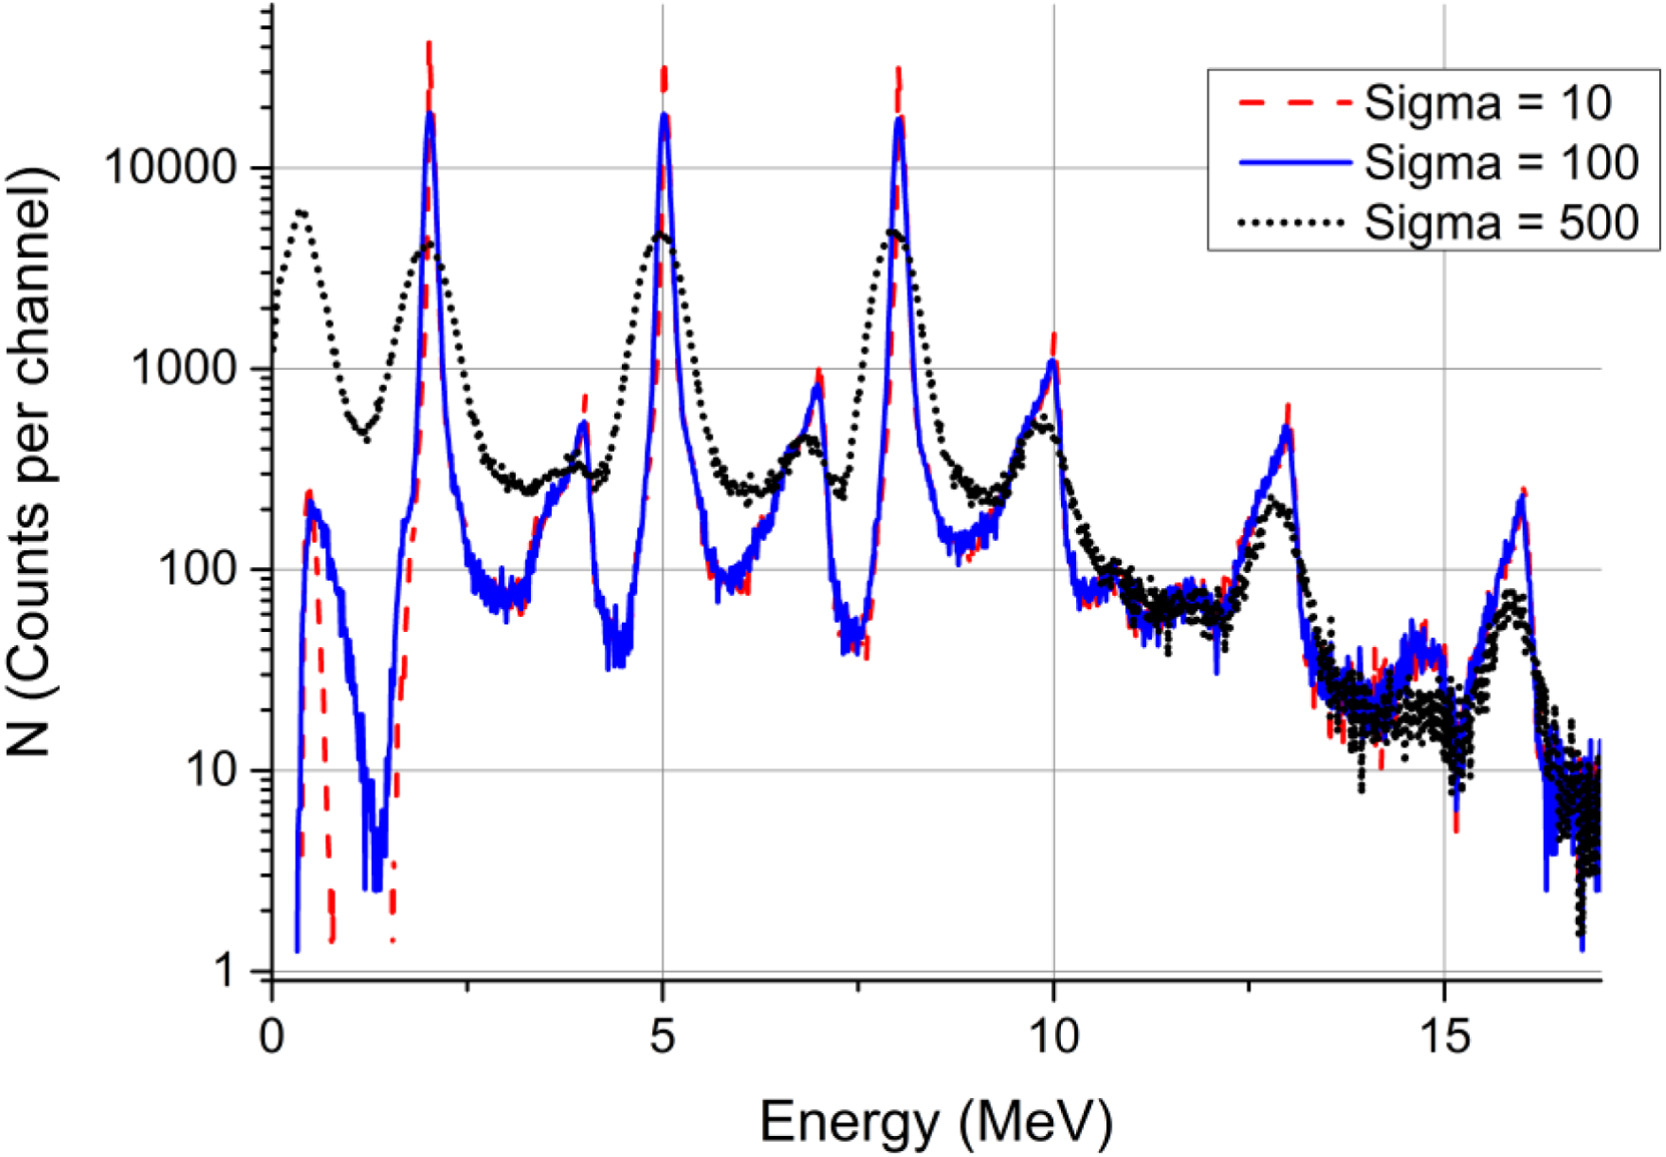
\includegraphics[width=0.65\linewidth]{processingSpectrumCmpByNoice} }
  \caption{ Спектры, полученные при обработке сигнала при нагрузке $10^7$~с${}^{-1}$ методом фиттинга с коррекцией спектра при различных значениях $\sigma_n$.~\cite{Khilkevitch2020} }
  \label{fig:processingSpectrumCmpByNoice}
\end{figure}


При уровне шума $\sigma_n \le 200$ количество отсчетов в пиках существенно не меняется при обработке любым из алгоритмов. При $\sigma_n = 500$ в отсутствие коррекции число событий на пиках, полученных при разделении импульсов, уменьшается. Это связано с тем, что ширина пика становится такой, что не все пиковые события попадают в энергетическое окно шириной 1~МэВ, как показано на рисунке~\ref{fig:processingSpectrumCmpByNoice}.

Полная ширина на полувысоте увеличивается в зависимости от уровня шума. При низких уровнях шума различия между алгоритмами практически несущественны. Однако при обработке алгоритмом <<по максимуму>> полуширина быстро линейно возрастает, что является очевидным свойством этого метода. Темпы роста ширины на полувысоте для спектров, полученных с помощью других алгоритмов, значительно ниже. Зависимость разрешения от уровня шума для спектров, полученных с помощью методов деконволюции и фиттинга, очень похожа.~\cite{Khilkevitch2020}

% ----------------------------------------------------------

\subsection{Время обработки сигнала}

Описанные выше алгоритмы имеют существенно разную алгоритмическую сложность. Время работы программы, в которой они были реализованы, зависит от конкретной программной реализации, аппаратной мощности компьютера, параметров обработки сигналов, а так же нагрузки детектора. Эти алгоритмы реализованы в компьютерном коде <<DeGaSum>>~\cite{Khilkevitch2020}. Код написан на языке программирования C++, а обработка происходит в несколько потоков с использованием SIMD-инструкций процессора.

\begin{figure}[ht!]
  \centerfloat{ 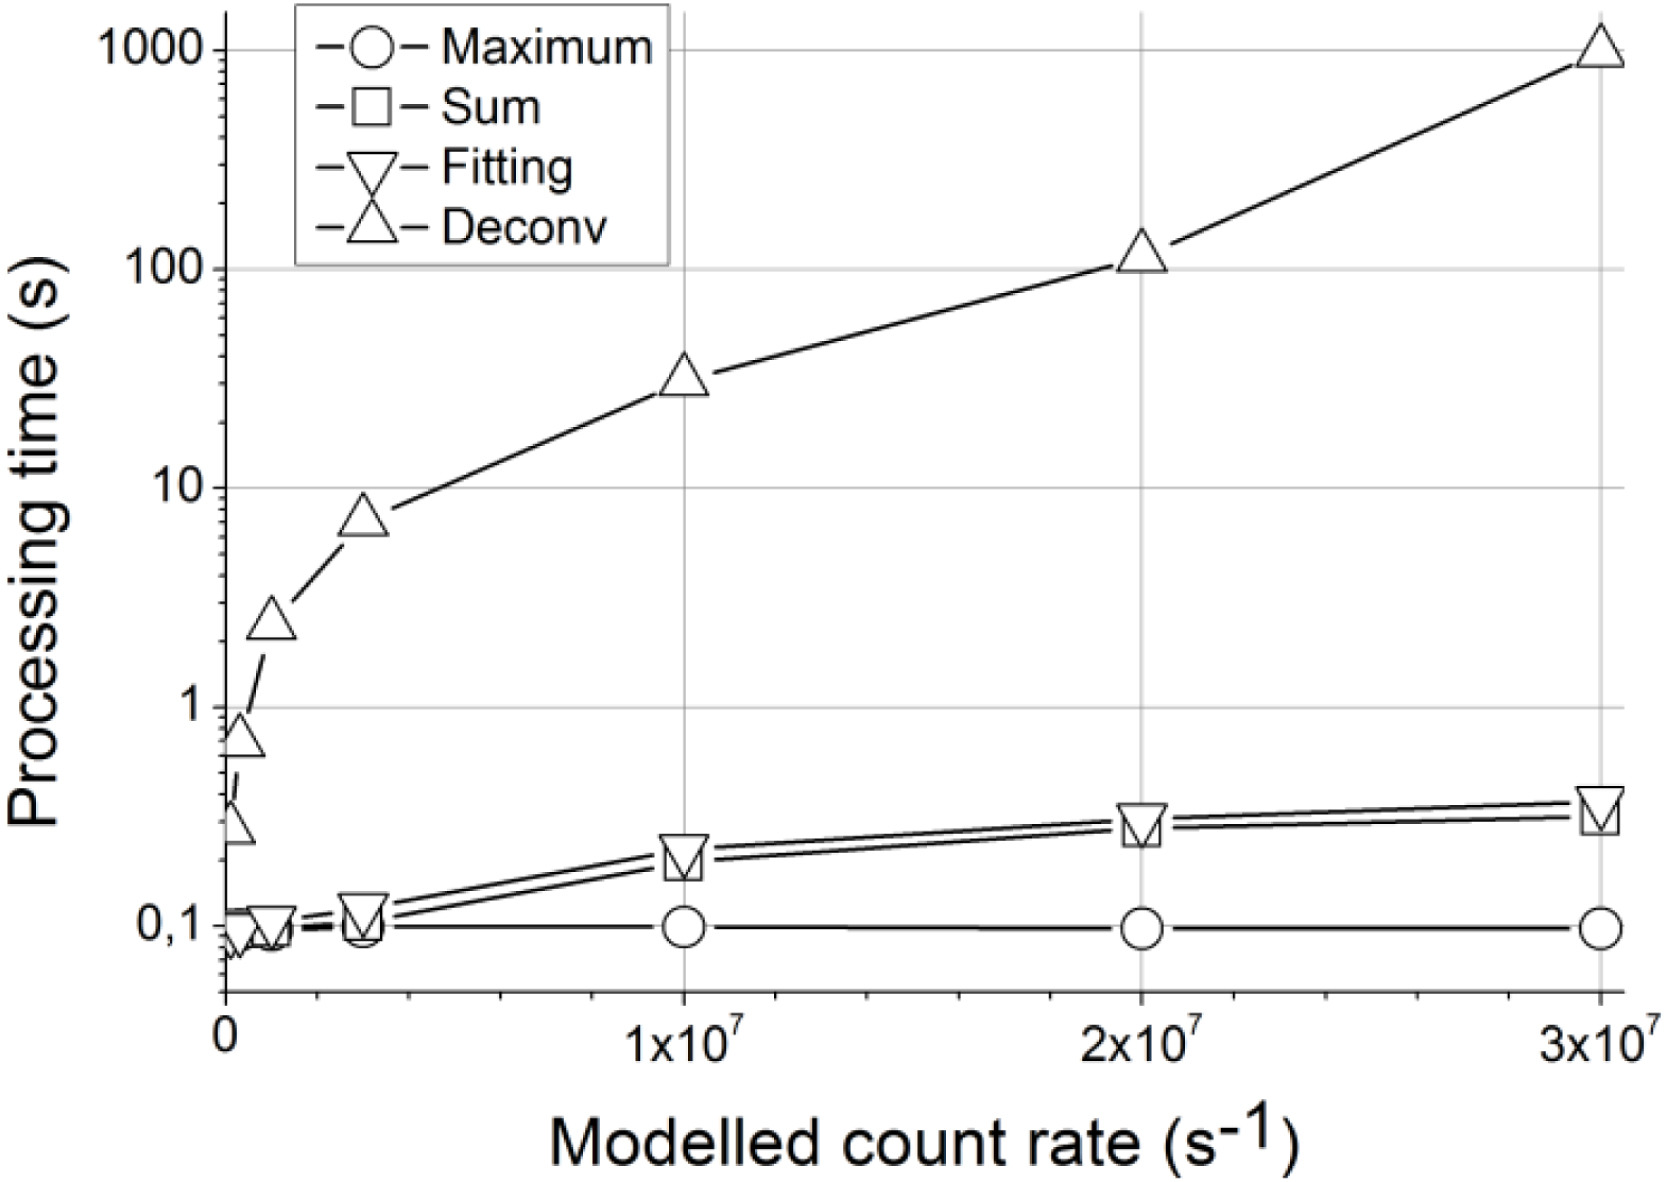
\includegraphics[width=0.65\linewidth]{processingTime} }
  \caption{ Время обработки смоделированного в разделе~\ref{sec:SignalGeneration} сигналов с использованием кода DeGaSum различными алгоритмами. В процессе обработки значение нулевой линии рассчитывалось по первым 10000 точкам сигнала. Модельный сигнал соответствуют длительности сбора данных 0.1~с при частоте дискретизации АЦП 250~МГц. Для обработки использовался ПК с процессором Intel Core i7-2700K@3.50~ГГц, 32~ГБ оперативной памяти, операционная система Debian Linux~10.4, код был скомпилирован с помощью g++~8.3.~\cite{Khilkevitch2020} }
  \label{fig:processingTime}
\end{figure}

На рисунке~\ref{fig:processingTime} показано время обработки модельного сигнала с использованием различных алгоритмов. Метод определения по максимум является простейшим вычислительным методом. Его производительность практически не зависит от загрузки детектора. Это связано с тем, что для его реализации необходим только последовательный поиск локальных максимумов. Другие методы требуют дополнительной обработки в областях, где значение сигнала превышает пороговый уровень, поэтому время их работы зависит от загрузки детектора. Метод деконволюции является наиболее затратным по вычислительным ресурсам, превосходя другие методы на порядки, особенно при больших нагрузках детектора. Это связано с тем, что его реализация требует дорогостоящих вычислительных операций для умножения матрицы и вектора.~\cite{Khilkevitch2020}

% ==========================================================

\section{Применение методов обработки на измеренных сигналах в экспериментах}

Для демонстрации работы алгоритмов был использован сигнал, полученный в ходе измерений, проведенных на циклотроне ФТИ им. А.Ф.~Иоффе~\cite{Lemberg1987}. Во время измерений пучок альфа-частиц направлялся на бериллиевую мишень, вызывая ядерную реакцию ${}^9Be(\alpha,n\gamma){}^{12}C$ с испусканием гамма-квантов с энергией 4,44~МэВ. Для измерений использовался сцинтилляционный детектор LaBr3(Ce) диаметром 76~мм с ФЭУ Hamamatsu R10233-100. Сигнал детектора оцифровывался с помощью платы АЦП ADP201X1/ADM214x400M/2A производства ЗАО <<Инструментальные системы>> с частотой дискретизации 250~МГц и записывался на жёсткий диск компьютера. Во время измерений менялся ток ионного пучка, что позволяло получать разные уровни загрузки детектора. Циклотрон работал в импульсном режиме.

\begin{figure}[ht!]
  \centerfloat{ 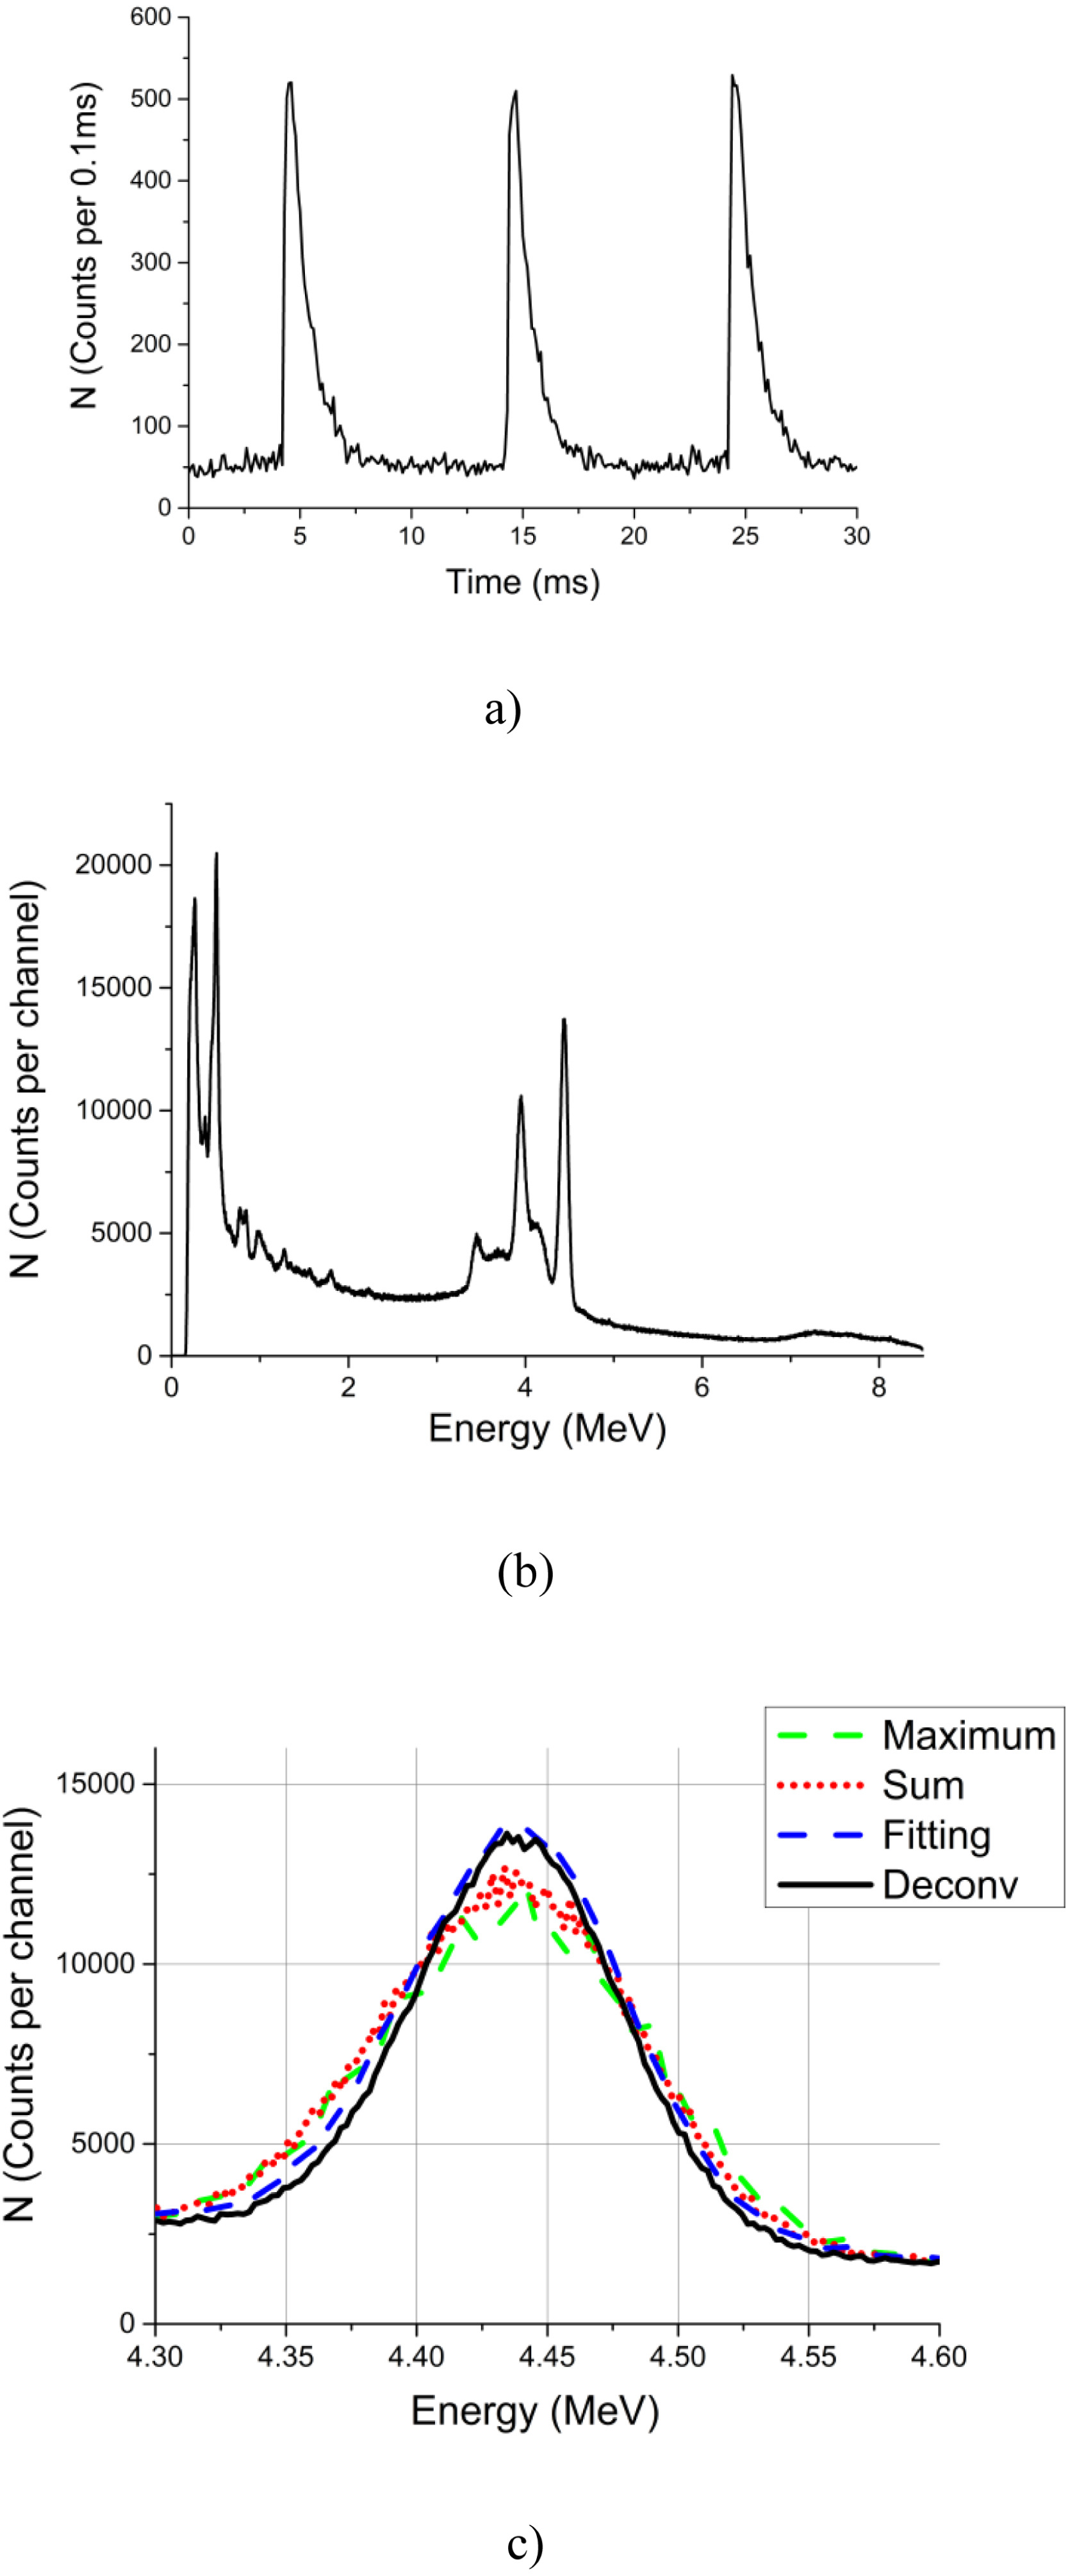
\includegraphics[width=0.51\linewidth]{processingCycloSignal} }
  \caption{ Результаты обработки сигнала, полученного в ходе измерений на циклотронне. a --- зависимость нагрузки детектора от времени (использовалась обработка методом фиттинга с коррекцией неразрешенных событий); b --- спектры гамма-излучения, полученные после обработки сигнала методом фиттинга; с --- cпектры гамма-излучения, полученные разными методами (построены вблизи пика 4.4~МэВ).~\cite{Khilkevitch2020} }
  \label{fig:processingCycloSignal}
\end{figure}

Результаты измерений представлены на рисунке~\ref{fig:processingCycloSignal}. Полная ширина на полувысоте (FWHM) пика 4.44~МэВ, полученная после обработки сигнала при максимальной нагрузке различными методами, представлена в таблице~\ref{tab:processingCycloSignal}. Видно что методы фиттинга и деконволюции имеют лучшее разрешение. Следует отметить, что линия 4.44~МэВ от реакции ${}^9Be(\alpha,n\gamma){}^{12}C$ уширена за счет эффекта Доплера. Доплеровская ширина линии для толстой бериллиевой мишени и пучка альфа-частиц с энергией 6~МэВ, ускоренного циклотроном, составляет примерно 51~кэВ.

\begin{table} [htbp]
    \centering
    \begin{threeparttable}
      \caption{ Полуширина пика с энергией 4.44~МэВ, полученная после обработки сигналов с использованием различных алгоритмов.~\cite{Khilkevitch2020} }
        \label{tab:processingCycloSignal}
        \begin{tabular}{| p{4cm} | p{6cm} | p{6cm} | }
            \hline
            Алгоритм   & Ширина линии, МэВ & \makecell{ Ошибка определения \\ ширины линии, МэВ } \\
            \hline
            По максимуму & 0.138 & 0.0019 \\
            Сумма &	0.135 &	0.0016\\
          Деконволюция &	0.093 &	0.0012 \\
          Фиттинг &	0.098 &	0.0012 \\
            \hline
        \end{tabular}
    \end{threeparttable}
\end{table}

С учетом эффекта Доплера рассчитанное энергетическое разрешение для линии 662~кэВ составило примерно 4.5\%. Однако следует отметить, что при таких нагрузках становится существенным эффект насыщения ФЭУ.

% ----------------------------------------------------------

\FloatBarrier
           % Глава 2
\chapter{Восстановление функции распределения убегающих электронов по измеренному спектру жёсткого рентгеновского излучения}
\label{ch:ch3}

% ==========================================================

\section{Восстановление исходного спектра гамма излучения по измеренному спектру}

В ходе применения описанных в главе~\ref{ch:ch2} процедур из записанной с помощью АЦП осциллограммы можно получить массив данных <<время-амплитуда>>, на основании которого построить спектр зарегистрированных событий. Однако полученный таким образом спектр не является спектром гамма-излучения, испущенным источником гамма квантов. 

Задача восстановления исходного распределения является весьма актуальной при обработке спектров и изображений в астрофизике~\cite{JungRichardt2016}, биологии и медицине~\cite{Vardi1985}, гамма и рентгеновской спектроскопии. Попытки восстановления исходного энергетического распределения из спектров, измеренных сцинтилляционными и полупроводниковыми детекторами, проводились ранее, например, в работах~\cite{Raad2008,Meng2000} и других.

Актуальность задачи привела к созданию большого числа различных методов деконволюции спектров и изображений. В ряде работ, например~\cite{Meng2000,Lanteri1999,Morhac2011,Jeffrey1986,Bouchet1995}, производилось сравнение между различными методами с целью выбрать наиболее подходящий для обработки спектров. Показано, что метод максимальной вероятной оценки с использованием ожидаемой максимизации (maximum likelihood estimation using expectation maximization, ML-EM)~\cite{Vardi1985}, известный так же как метод Ричардсона-Луси~\cite{Richardson1972,Lucy1974}, является одним из лучших при восстановлении гамма спектров: он демонстрирует хорошую устойчивость к шумам исходных данных и позволяет сравнительно точно восстанавливать исходные спектры~\cite{Meng2000,Morhac2011}.

Во всех упомянутых работах методы деконволюции применялись к случаю, когда исходный спектр является дискретным. Кроме того, предполагалась большая статистика спектров. В то же время спектры, получаемые в экспериментах на токамаках, обычно имеют весьма малую статистику~(\cite{Khilkevitch2013,Shevelev2018,Reux2022,Chugunov2011,Shevelev2013} и другие). Помимо этого, в спектрах зачастую присутствует вклад нейтронного излучения. Спектры жёсткого рентгеновского излучения, генерируемые убегающими электронами, почти всегда имеют непрерывный характер~\cite{Shevelev2013}. Всё это усложняет применение описанных выше алгоритмов к экспериментальным данным.~\cite{Khilkevitch2013} 

В этой главе описаны методы, с помощью которых возможно на основе измененных амплитудных спектров событий, зарегистрированных с помощью детекторов, восстановить энергетические спектры гамма излучения; кроме того, будет описано применение методов для восстановления функции распределения убегающих электронов по энергии.

% ==========================================================

\section{ Восстановление спектра гамма излучения по измеренному спектру излучения }

% ----------------------------------------------------------

\subsection{ Использование метода ML-EM для восстановления спектра излучения }

Измеренный с помощью гамма детектора спектр $s(\varepsilon)$ может быть представлен в следующем виде:
\begin{equation}
  \label{eq:BaseConvolution}
  s(\varepsilon) = \int \limits_0^{+\infty} g( \varepsilon' ) h( \varepsilon, \varepsilon' ) d \varepsilon' + n(\varepsilon)
\end{equation}
где $g(\varepsilon)$ --- спектр гамма излучения от источника излучения, $n(\varepsilon)$ --- статистический пуассоновский шум, $ h( \varepsilon, \varepsilon' ) $ --- передаточная функция, $\varepsilon$ --- энергия. Задача восстановления заключается в нахождении спектра гамма излучения $g$ по измеренному спектру $s$ при известной передаточной функции $h$.~\cite{Khilkevitch2013}

Для решения уравнения~\ref{eq:BaseConvolution} необходимо знать функцию $ h( \varepsilon, \varepsilon' ) $. Это --- передаточная функция, её физический смысл следующий: для моноэнергетического пучка гамма квантов с энергией $\varepsilon'$, испускаемый источником, с помощью детектора будет зарегистрирован спектр, равный $s(\varepsilon) = h(\varepsilon, \varepsilon') \cdot N_{\gamma}$ без учёта шума, где $N_{\gamma}$ --- количество гамма квантов, испущенных источником. Передаточная функция $h$ зависит от характеристик самого детектора (площади, материала, эффективности, относительного влияния на зарегистрированный спектр таких эффектов как комптоновское рассеяние, интенсивности пиков полного поглощения, одиночного и двойного вылета, и тому подобное), от процессов, произошедших с квантом после его испускания на пути к детектору (поглощение в конструкциях, размещённых на пути гамма кванта от источника к детектору, отражение от окружающих конструкций, и так далее), от распределения испускаемого излучения по углам и от геометрического расположения детектора относительно источника гамма квантов. Функция $h$ может быть измерена экспериментально, однако на практике проще получить её с помощью численного моделирования с помощью одного из кодов, например с помощью компьютерного кода MCNP (Monte Carlo N-Particle code) и программы MCAM (Monte Carlo Automatic Modeling Program for Radiation Transport Simulation)~\cite{Hendricks2004,Fischer2005,Wu2009}.

Задачи определения неизвестного $x$ вида 
\begin{equation*}
  y = A x, x \in X, y \in Y
\end{equation*}
где $X$ и $Y$ --- некоторые пространства, $A$ --- оператор: $ A : X \rightarrow Y $, называются корректными по Адамару, если для каждого фиксированного $y$ решение $x$ существует, единственно и устойчиво. Под устойчивостью тут подразумевается то, что при малом изменении $y$ значение решения $x$ так же изменится мало~\cite{Liskovets1982}. Решение уравнения~\ref{eq:BaseConvolution} представляет собой некорректно поставленную по Адамару задачу, близкую к задаче деконволюции. Для решения подобного класса задач известен целый ряд методов, часть из которых могут быть применены и в задачах гамма-спектрометрии.

Уравнение~\ref{eq:BaseConvolution} можно переписать в дискретной форме:
\begin{equation}
  \label{eq:BaseConvolutionMatrix}
  s = H \cdot g + n 
\end{equation}
где $s$, $g$, $n$ --- вектора, $H$ --- матрица. Для выбранной дискретной сетке по энергиям размерностью $N$ в интервале $ \varepsilon_0 \ldots \varepsilon_N $ элементы векторов оказываются равными значениям
\begin{equation*}
  s_i = \int \limits_{\varepsilon_i}^{\varepsilon_{i+1}} s( \varepsilon' ) d \varepsilon'
\end{equation*}
Для простоты можно считать, что эта сетка одинаковая для измеренного спектра и исходного спектра гамма излучения, но в общем случае это может быть и не так

Метод ML-EM \cite{Vardi1985,Richardson1972,Lucy1974} может быть применён для решения уравнений вида \ref{eq:BaseConvolutionMatrix}.~\cite{Khilkevitch2013,Shevelev2013} Это итеративный алгоритм, на каждой итерации следующее значение вычисляется как
\begin{equation*}
  g_i^{p+1} = g_i^p \cdot \sum \limits_{j = 0 }^{N} h_{j,i} \frac{ s_j }{ \sum \limits_{k=0}^{N} h_{j,k} g_k^p }
\end{equation*}
где верхний индекс $p$ --- номер итерации. На каждом шаге алгоритма выполняется преобразование 
\begin{equation*}
  g_i^p = \max \left( g_i^p, 0 \right)
\end{equation*}
которое обеспечивает неотрицательность решения --- очевидно, что искомая интенсивность гамма излучения не может быть отрицательной. В качестве начального приближения для работы алгоритма можно использовать значение
\begin{equation*}
  g^0 = \frac{ s }{ \| H s \| }
\end{equation*}
где $ \| H s \| $ --- норма вектора $ H s $. Условие для окончания работы алгоритма можно задать следующим образом:
\begin{equation*}
  \| s - H g^{p-1} \| - \| s - H g^p \| < \epsilon \cdot N
\end{equation*}
где $\epsilon$ --- параметр алгоритма.~\cite{Shevelev2013} 

Базовый алгоритм может быть модифицирован. В задачах гамма-диагностики о функции $g$ обычно имеется хотя бы минимальная априорная информация. Так, для спектра излучения, который образуется в результате ядерных реакций, присутствует ряд дискретных линий. Эти линии могут быть уширены за счёт доплеровского уширения линий. Для такого спектра можно использовать процедуру, основанную на работе~\cite{Morhac2011} и модифицированную в~\cite{Khilkevitch2013,Shevelev2013}: на каждом k-том шаге проводить <<вытягивание>> линий с помощью процедуры
\begin{equation}
  \label{eq:BoostMlemDisturb}
  g^{p, boost}_i = \left( g^p_i \right)^{\beta} \cdot \frac{ \sum_j g^p_i }{ \sum_j g^{p, boost}_j }
\end{equation}
где значение степени $\beta$ --- параметр алгоритма, он должен быть чуть больше 1.0 (например, 1.01). 

Спектр излучения, генерируемого убегающими электронами, обычно имеет непрерывный характер. В это случае предлагается использовать другую модификацию: на каждом l-ом шаге сглаживать полученное решение. Можно использовать линейное сглаживание с весом:
\begin{equation*}
  g^{p, smooth}_i = w \cdot \left( g^p_{i-1} + g^p_i + g^p_{i+1} \right)/3 + ( 1 - w ) \cdot g^p_i
\end{equation*}
где коэффициент $w$ --- параметр алгоритма. Тут использовано сглаживание по трём точкам, но аналогично можно использовать линейное сглаживание по пяти или семи точкам, или другие способы сглаживания.~\cite{Khilkevitch2013} При линейном сглаживании необходимо обратить внимание на следующую особенность функции отклика $h$, используемую при восстановлении функции распределения убегающих электронов: электроны с энергией $\varepsilon_e$ генерируют гамма кванты с энергией преимущественно $\varepsilon_{\gamma} \ll \varepsilon_e$. Это приводит к тому, что значение вектора $g_i$ определяется с очень большой ошибкой при малых значениях индекса $i$; а процедура сглаживания приводит к нежелательному распространению этой ошибки в область больших энергий. Для того, чтобы этого избежать, в некоторых случаях имеет смысл сглаживать промежуточное решение только начиная с некоторого $i_{smooth} > 0$, значение которого --- параметр алгоритма (обычно в районе 10--20)~\cite{Khilkevitch2013}.

В случае, если искомая функция $g$ имеет смешанный характер, то есть содержит как гладкую непрерывную часть, так и дискретные пики, восстановление становится особенно сложным, поскольку решение имеет тенденцию к осцилляциям. В этом случае приходится эврестически подбирать параметры выполнения процедуры восстановления.

Для определения ошибок определения амплитуды может быть применён метод Монте-Карло~\cite{Shirk1985}. Для этого генерируется $M$ наборов векторов 
\begin{equation*}
  {{s'}_i}^{m} = R^{psn}(s_i)
\end{equation*}
где $ R^{psn}(x) $ --- случайное число с пуассоновским распределением и среднем значением $x$. Затем для каждого вектора ${s'}^{m}$ ищется соответствующее ему решение ${g'}^{m}$ с помощью описанного выше алгоритма ML-EM. Затем ищутся величины
\begin{equation*}
  \Delta_i = \sqrt{ \frac{1}{M} \sum \limits_{ m = 0 }^{M} \left( {g'_i}^{m} - g_i \right)^2 }
\end{equation*}
которые представляют собой среднеквадратичные отклонения для найденного решения $g$.~\cite{Shevelev2013}

Описанный выше алгоритм реализован в программном коде <<DeGaSum>>.~\cite{Khilkevitch2013}

% ----------------------------------------------------------

\subsection{ Проверка корректности восстановления и отработка методики для калибровочных источников излучения }

Для проверки корректности было проведено несколько экспериментов в лабораторных условиях с использованием калибровочных источников с известной интенсивностью излучения. 

В первом эксперименте использовались источники ${}^{60}$Co и ${}^{137}$Cs. Для восстановления спектра необходимо предварительно провести расчеты аппаратных функций детектора с реалистичными геометрическими и техническими параметрами в широком диапазоне энергий с как можно меньшими шагами по энергии, а так же рассчитать эффекты, возникающие при движении гамма кванта к детектору. Примеры аппаратных функций сцинтилляционного детектора, рассчитанных по программе MCNP (Monte-Carlo N-Particle), представлены на рисунке~\ref{fig:mcnpInstFunctionsNaI}; расчёты выполнял А.~Е.~Шевелев. Расчёты проводились для коллимированного пучка гамма-излучения. Полученные спектры нормировались на число гамма-квантов, вышедших из модельного источника, и ширину шага по энергии. В спектрах можно увидеть большие пики полного поглощения энергии, более мелкие пики одинарного вылета и непрерывные участки, соответствующие комптоновскому рассеянию гамма-излучения. Пики двойного вылета очень малы из-за большого размера и высокой эффективности сцинтилляционного кристалла. Моделирование проводилось для детектора NaI(Tl) размером $\varnothing$127$\times$152~мм с энергетическим разрешением 7\% на линии 662~кэВ. Использование детектора NaI(Tl) обусловлено желанием проверить алгоритм в более сложных условиях, используя детектор с заведомо низким разрешением по сравнению с более современными детекторами LaBr3(Ce).

\begin{figure}[ht!]
  \centerfloat{ 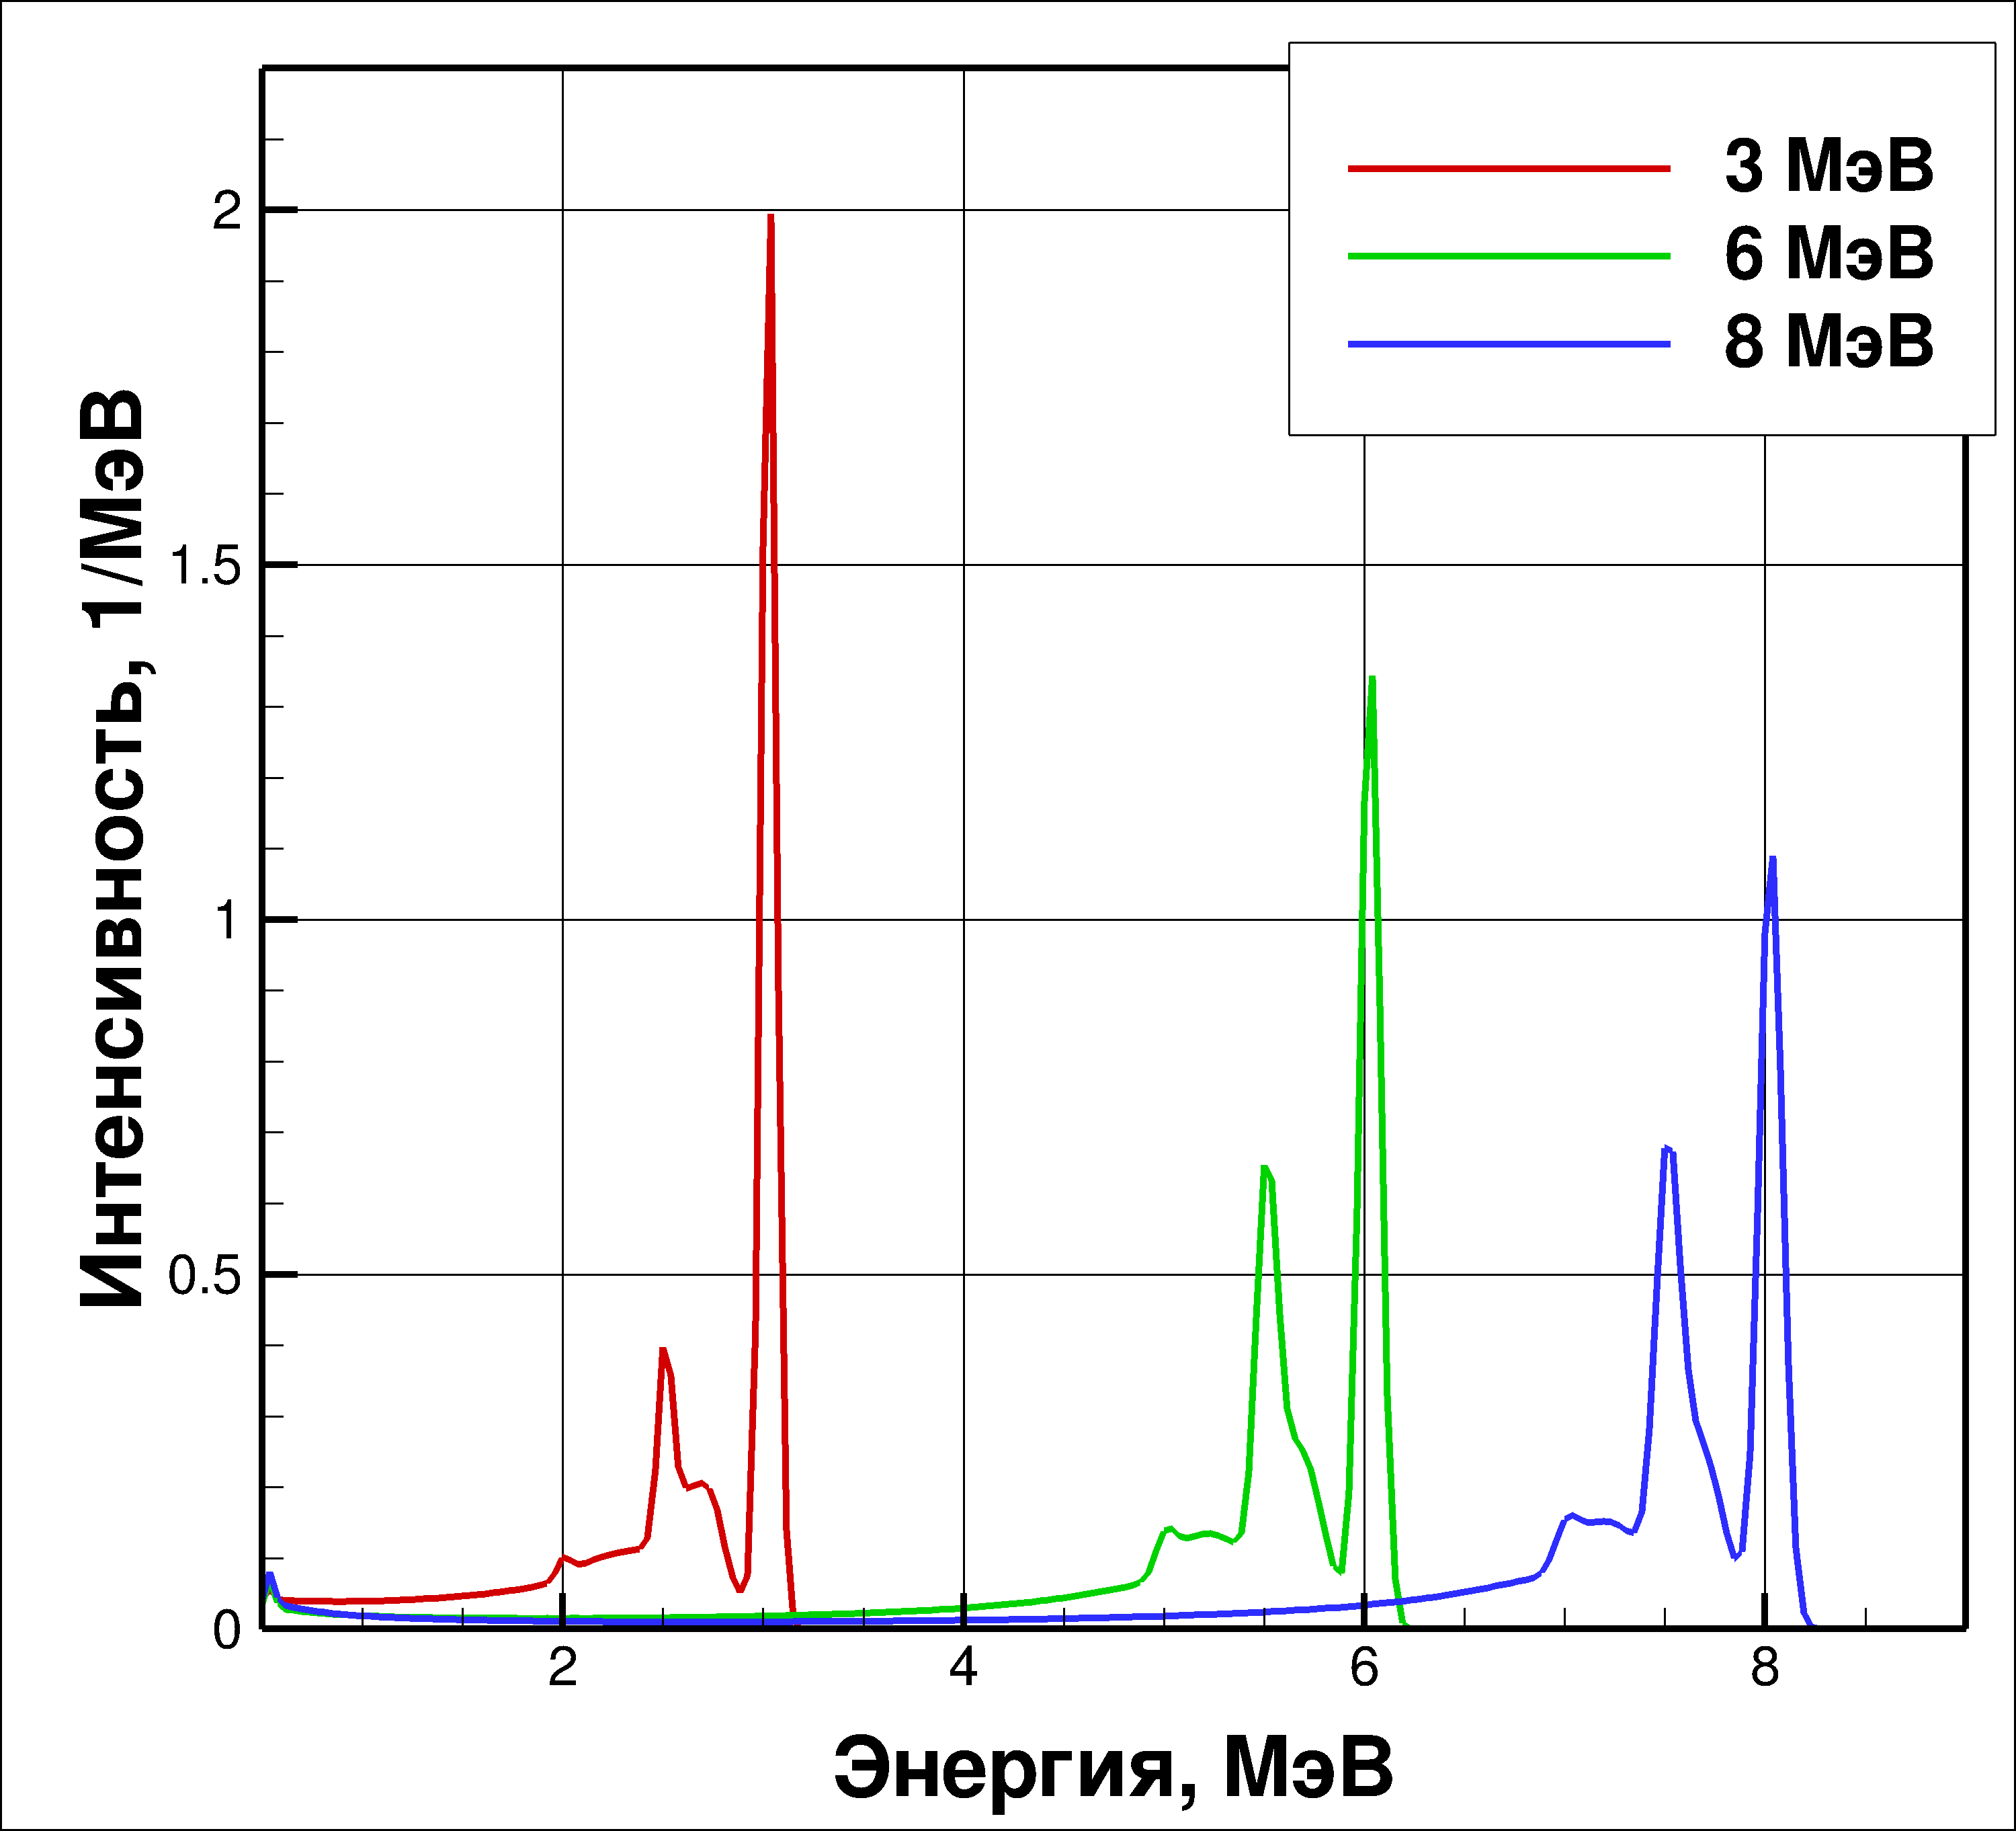
\includegraphics[width=0.52\linewidth]{mcnpInstFunctionsNaI} }
  \caption{ Примеры аппаратных функций, рассчитанных с помощью кода MCNP для детектора NaI(Tl) для различных значений энергии поглощаемых гамма квантов.~\cite{Shevelev2013} }
  \label{fig:mcnpInstFunctionsNaI}
\end{figure}

Были проведены измерения с использованием детектора NaI(Tl) размером $\varnothing$150$\times$100~мм с энергетическим разрешением 11,5\% на линии 661.6~кэВ. Функции отклика этого детектора рассчитывались по программе MCNP в диапазоне энергий 60--3000~кэВ с шагом 20~кэВ; расчёты выполнял А.~Е.~Шевелев. В разработанной расчетной модели источник изотропного гамма-излучения располагался на расстоянии 25.5~см от детектора. На одинаковом расстоянии от реального детектора для проведения измерений были установлены радиоактивные источники ${}^{60}$Co и ${}^{137}$Cs с известной активностью распада. Результаты обработки измеренного спектра показаны на рисунке~\ref{fig:cocsReconstructIoffe}. Время набора первого спектра составляет 150~секунд, время набора второго спектра --- 2~секунды, оба спектра были набраны в одинаковой геометрии. Обработка второго спектра иллюстрирует способность алгоритма работать с данными с низкой статистикой. Количество событий в восстановленных пиках соответствует количеству гамма-квантов, испущенных радиоактивными источниками во время регистрации спектра. Применяемая методика позволила определить активность радиоактивных источников с точностью 1.5\% для спектра с временем набора 150~секунд и 2.4\% для спектра с временем набора 2~секунды.~\cite{Shevelev2013}

\begin{figure}[ht!]
    \begin{minipage}[b][][b]{0.95\linewidth}\centering
        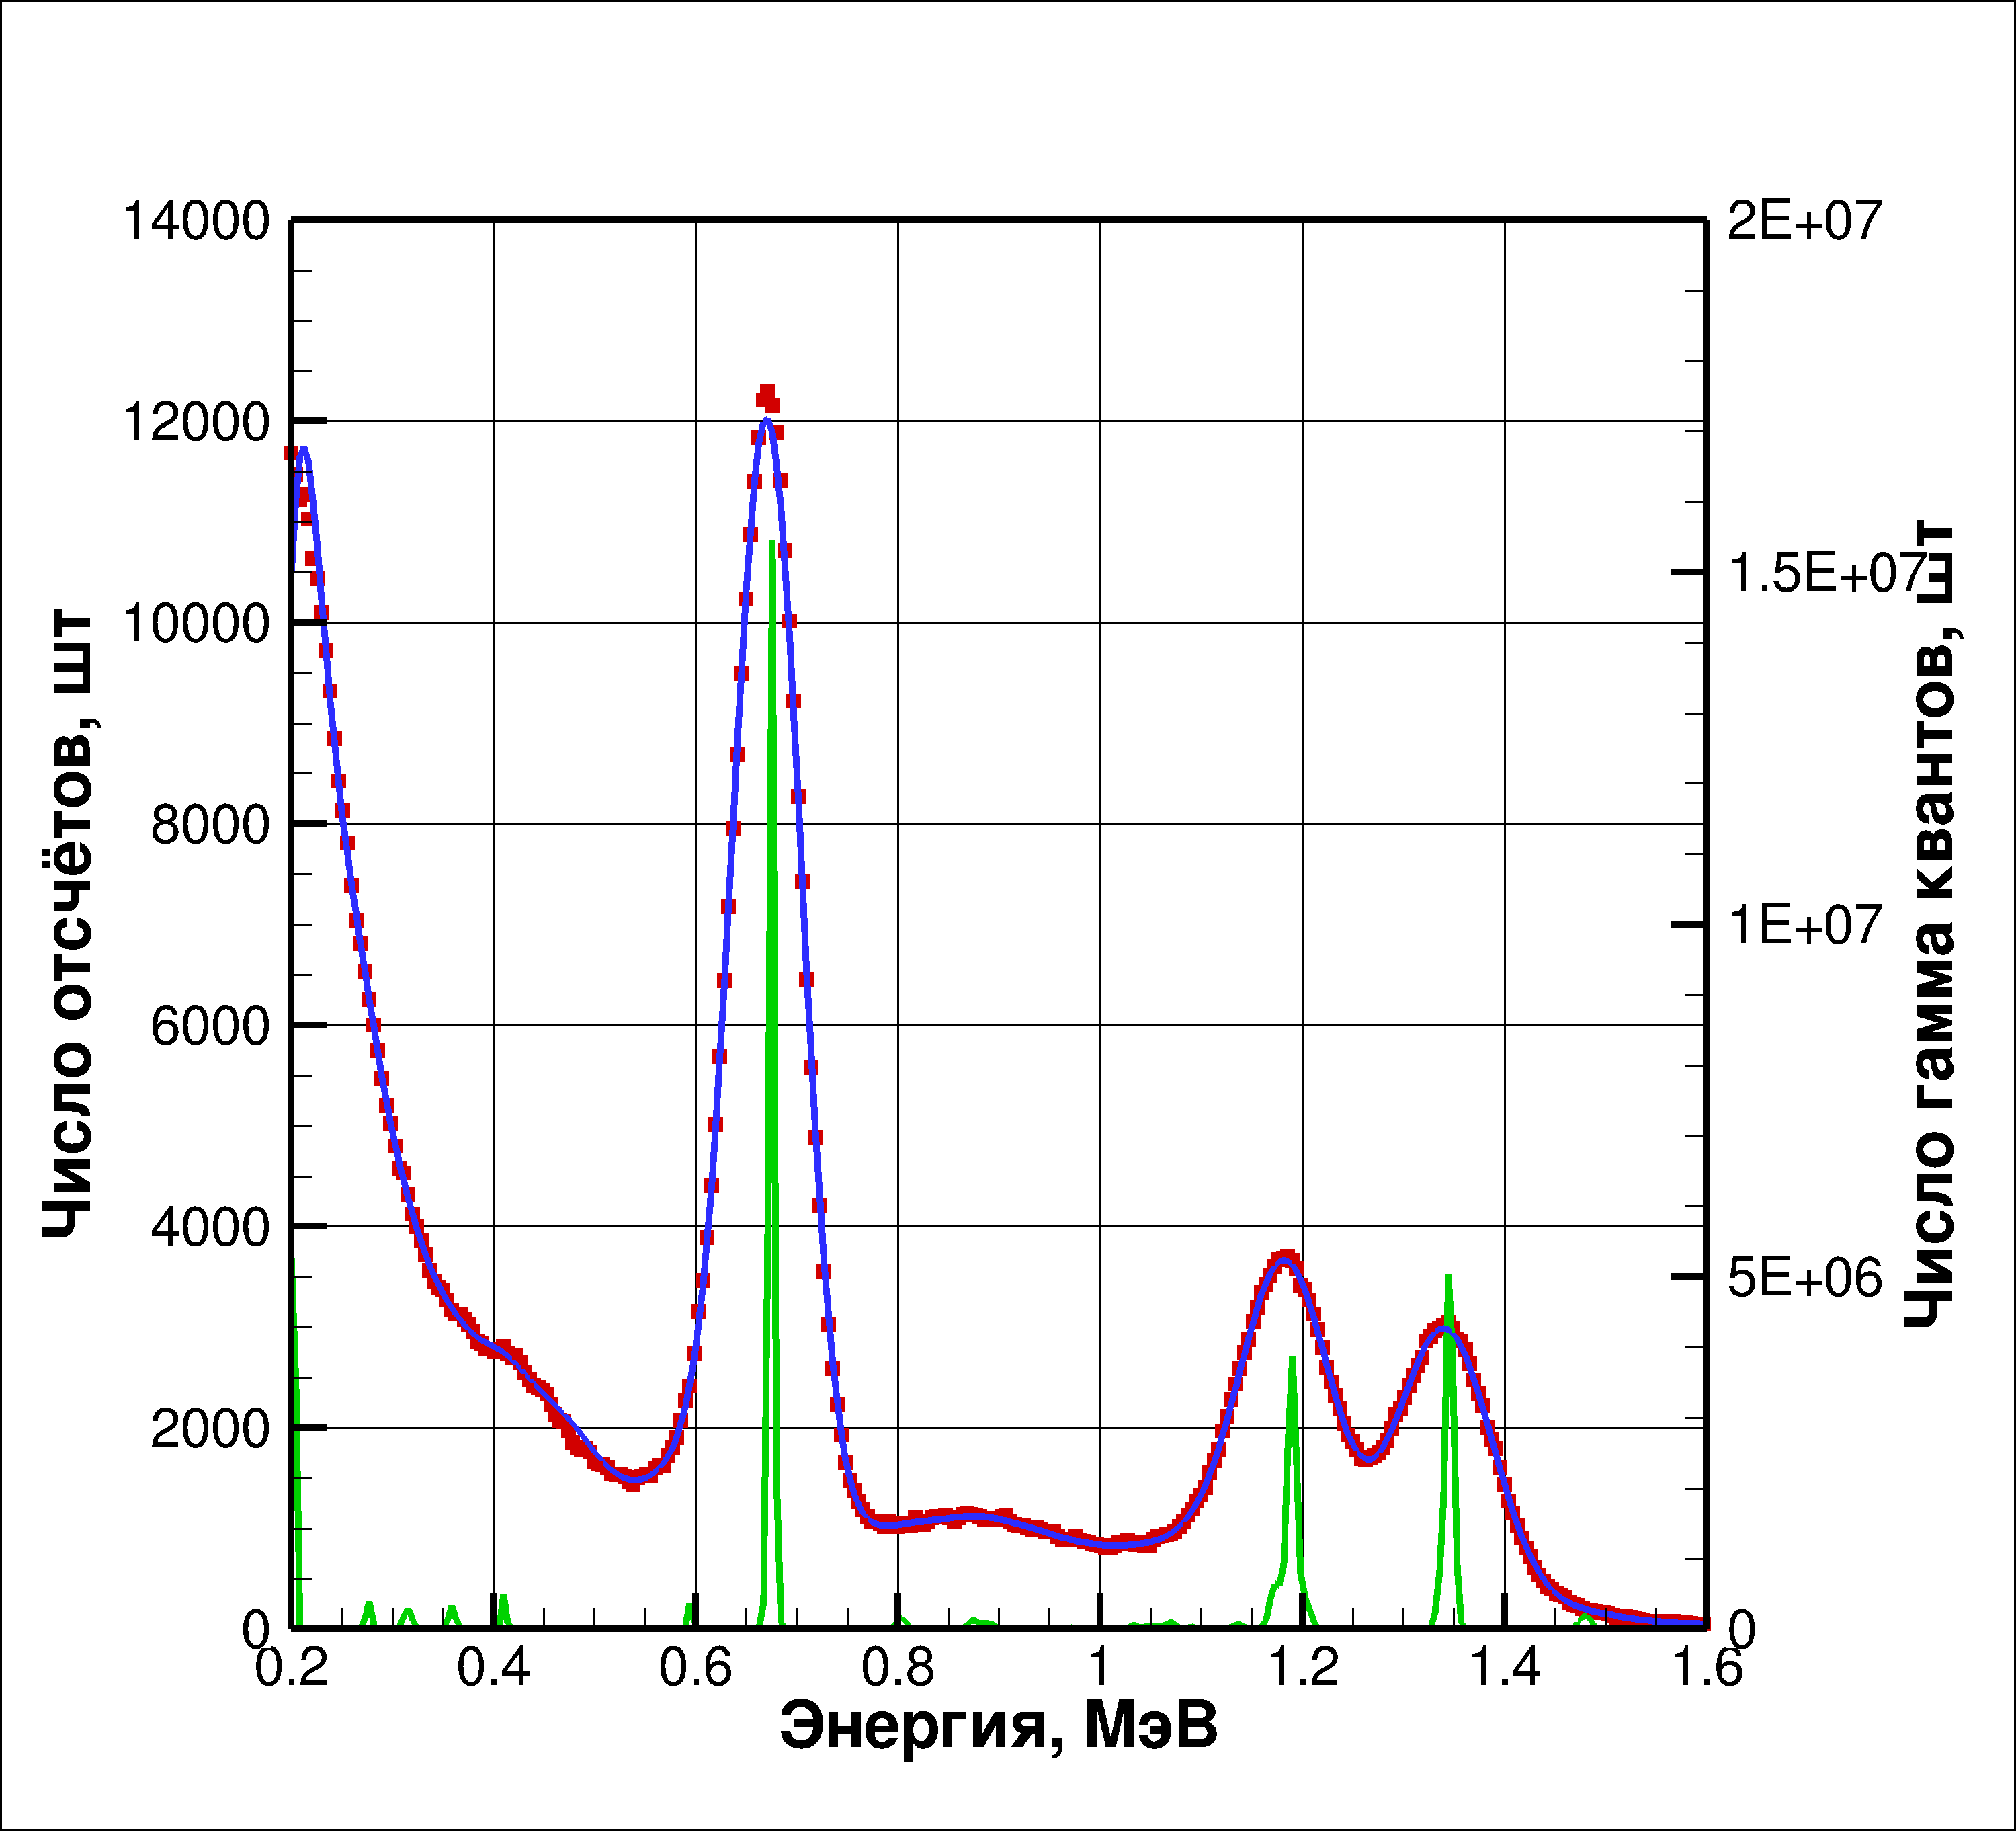
\includegraphics[width=0.52\linewidth]{cocsReconstructIoffe300s} \\ а) \\
    \end{minipage}
    \vfill
    \begin{minipage}[b][][b]{0.95\linewidth}\centering
        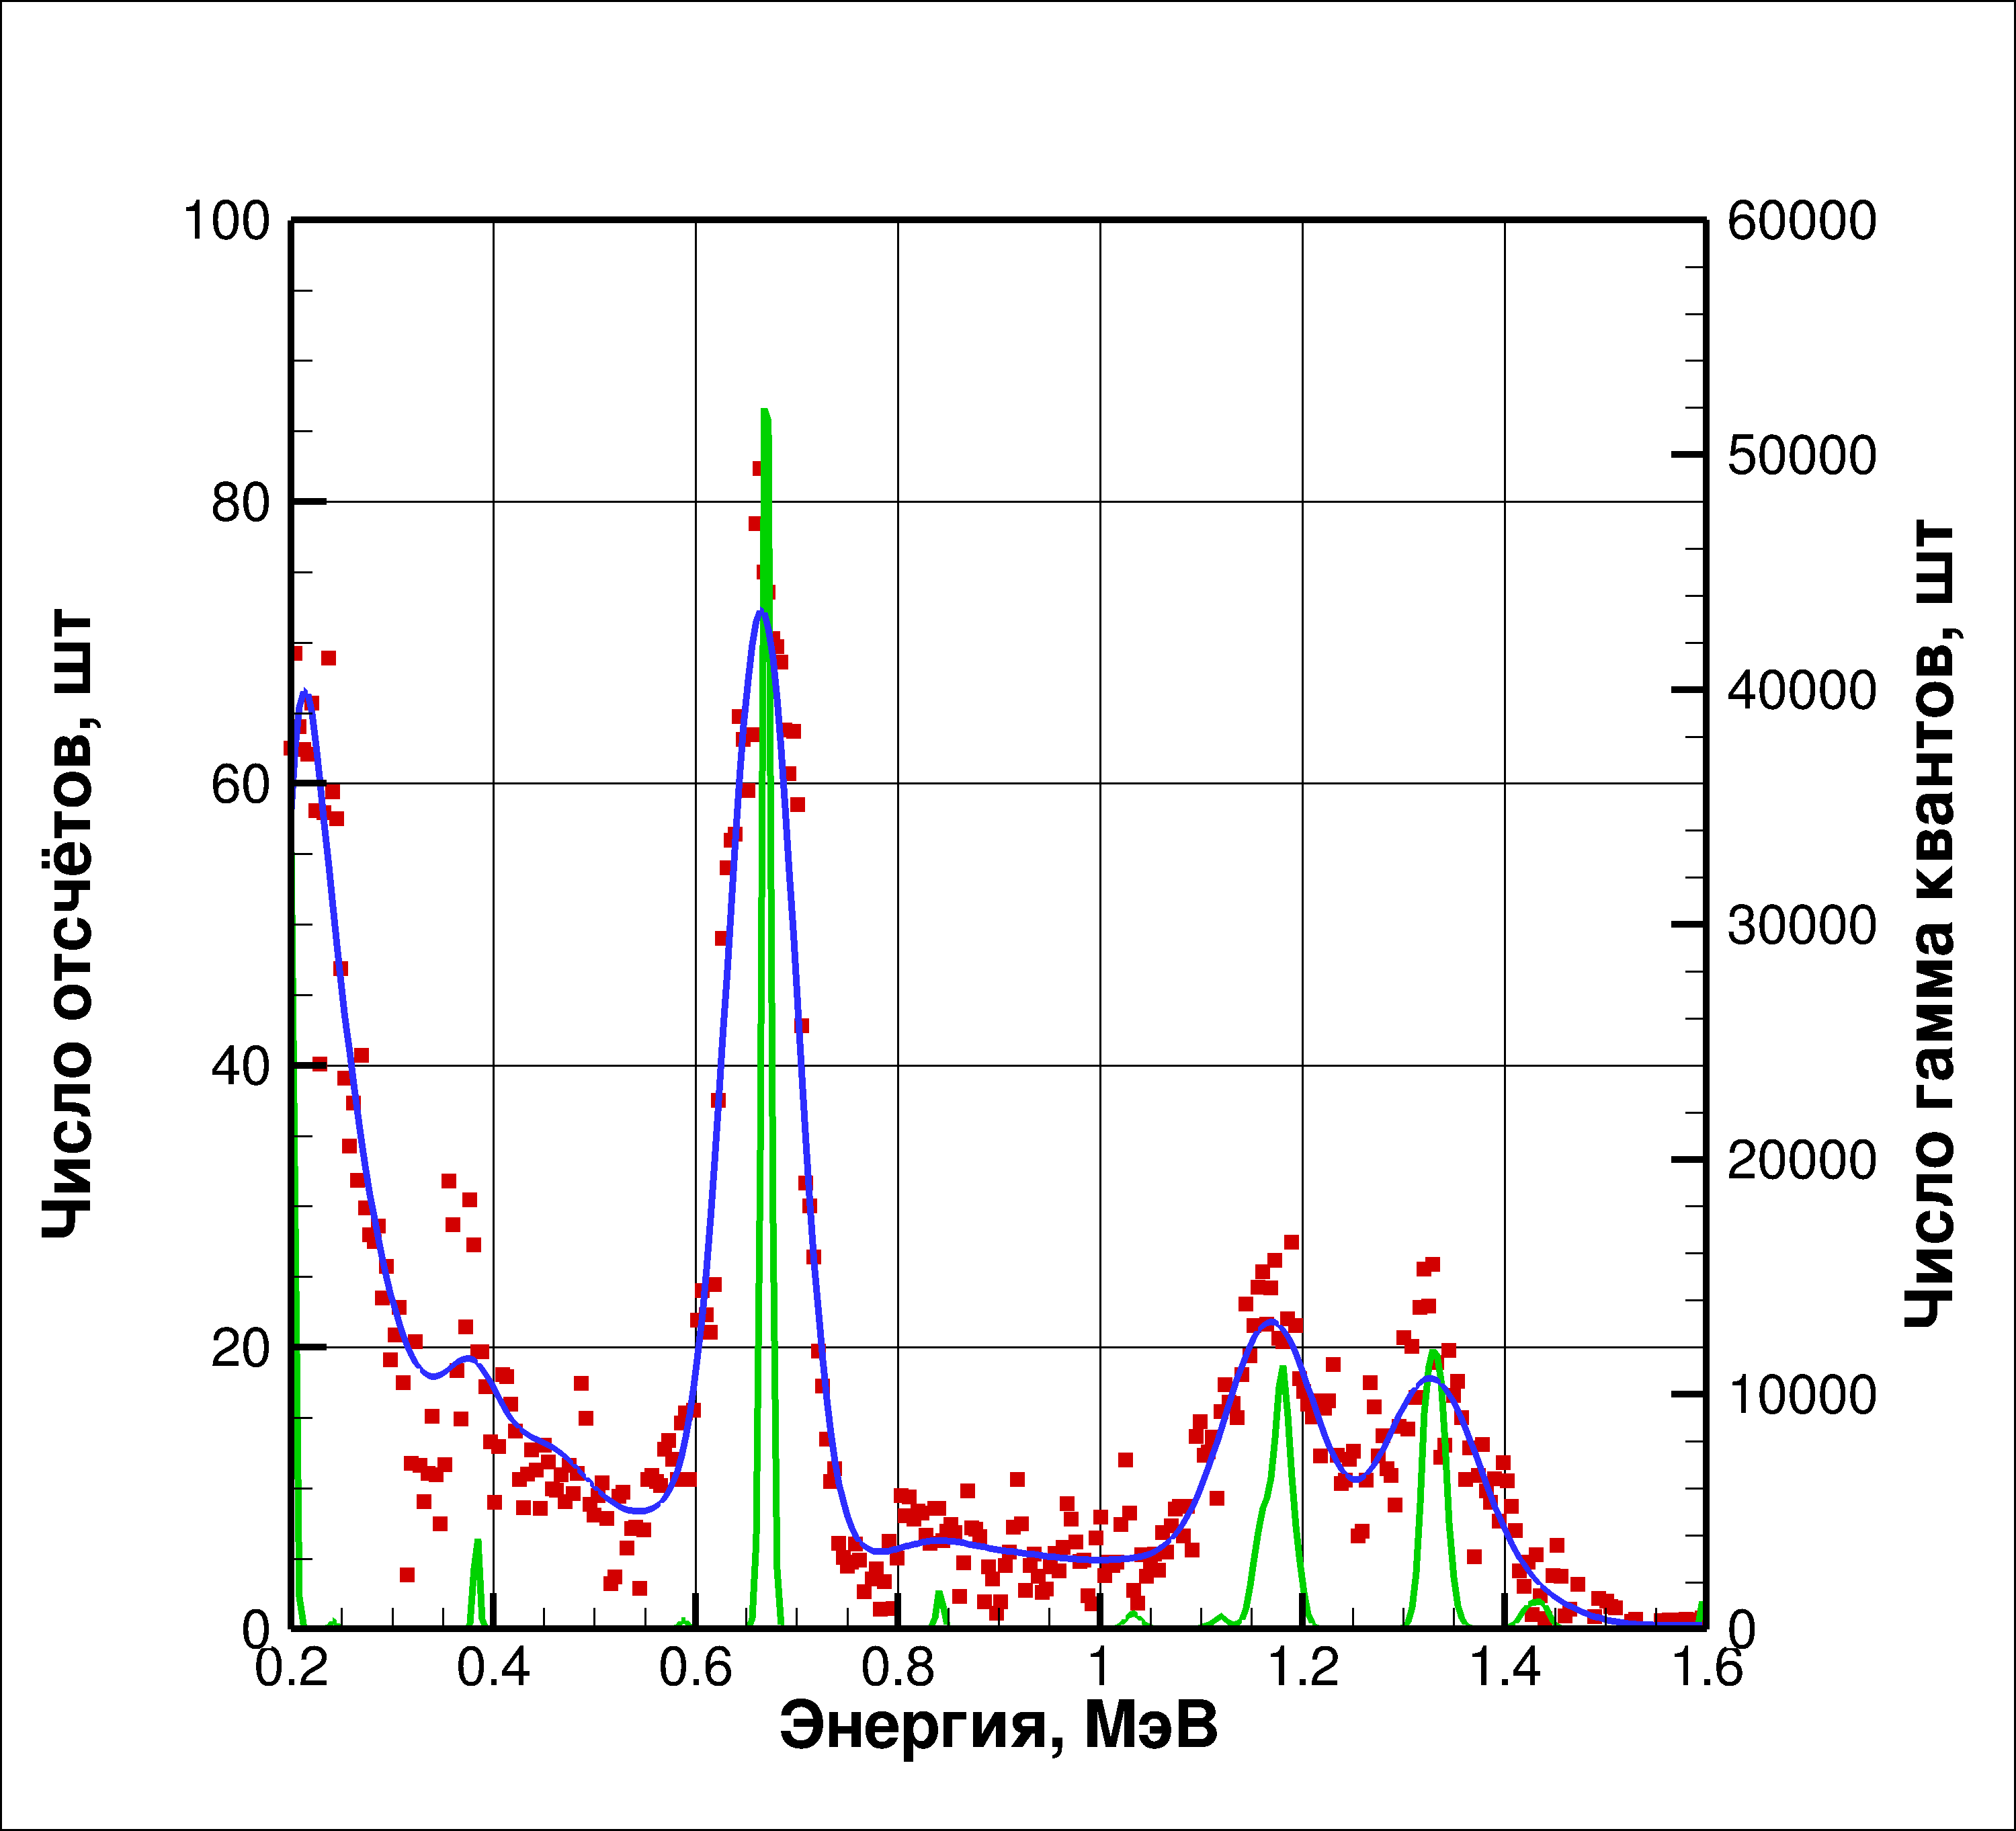
\includegraphics[width=0.52\linewidth]{cocsReconstructIoffe2s} \\ б) \\
    \end{minipage}
    \vspace{5mm}
    \caption{ Спектр источников ${}^{60}$Co и ${}^{137}$Cs, время набора 150 секунд (а) и 2 секунды (б). Красной линией показан измеренный детектором спектр, зелйной линией --- восстановленный спектр источников гамма излучения, синим --- результат <<прямой свёртки>>, интегрирования восстановленного спектра с передаточной функцией детектора (аппаратной функцией с учётом геометрии источника и детектора). В случае идеального восстановления спектра синяя кривая должна совпадать с красными точками.~\cite{Shevelev2013}. }
    \label{fig:cocsReconstructIoffe}
\end{figure}
\FloatBarrier

В другом эксперименте в измерениях использовался тот же самый NaI(Tl) детектор с размерами $\varnothing$150$\times$100~мм. Использовался источник гамма-излучения ${}^{152}$Eu с известной активностью распада. Результат обработки спектра источника ${}^{152}$Eu показан на рисунке~\ref{fig:euReconstructedSpectrum} и в таблице~\ref{tab:euReconstructedLines}. Из этого спектра был предварительно вычтен измеренный спектр фонового излучения. Восстановленный спектр позволил определить все основные линии источника ${}^{152}$Eu. Ошибка определения линий с высокой интенсивностью оказывается сравнительно небольшой. Она может быть объяснена  неточным  определением расстояния до источника. Метод позволил выявить линии с крайне малой интенсивностью 1.212~МэВ, 1.299~МэВ, 0.688~МэВ, 0.586~МэВ, 0.563~МэВ, невидимые в исходном спектре, хотя и с большой относительной ошибкой при определении амплитуды. Удалось обнаружить так же невидимую в исходном спектре линию 0.867~МэВ и сравнительно точно определить её интенсивность. Удалось разрешить близко расположенные пары линий 0.411 и 0.444~МэВ, 1.085 и 1.112~МэВ.~\cite{Khilkevitch2013}

\begin{figure}[ht!]
  \centerfloat{ 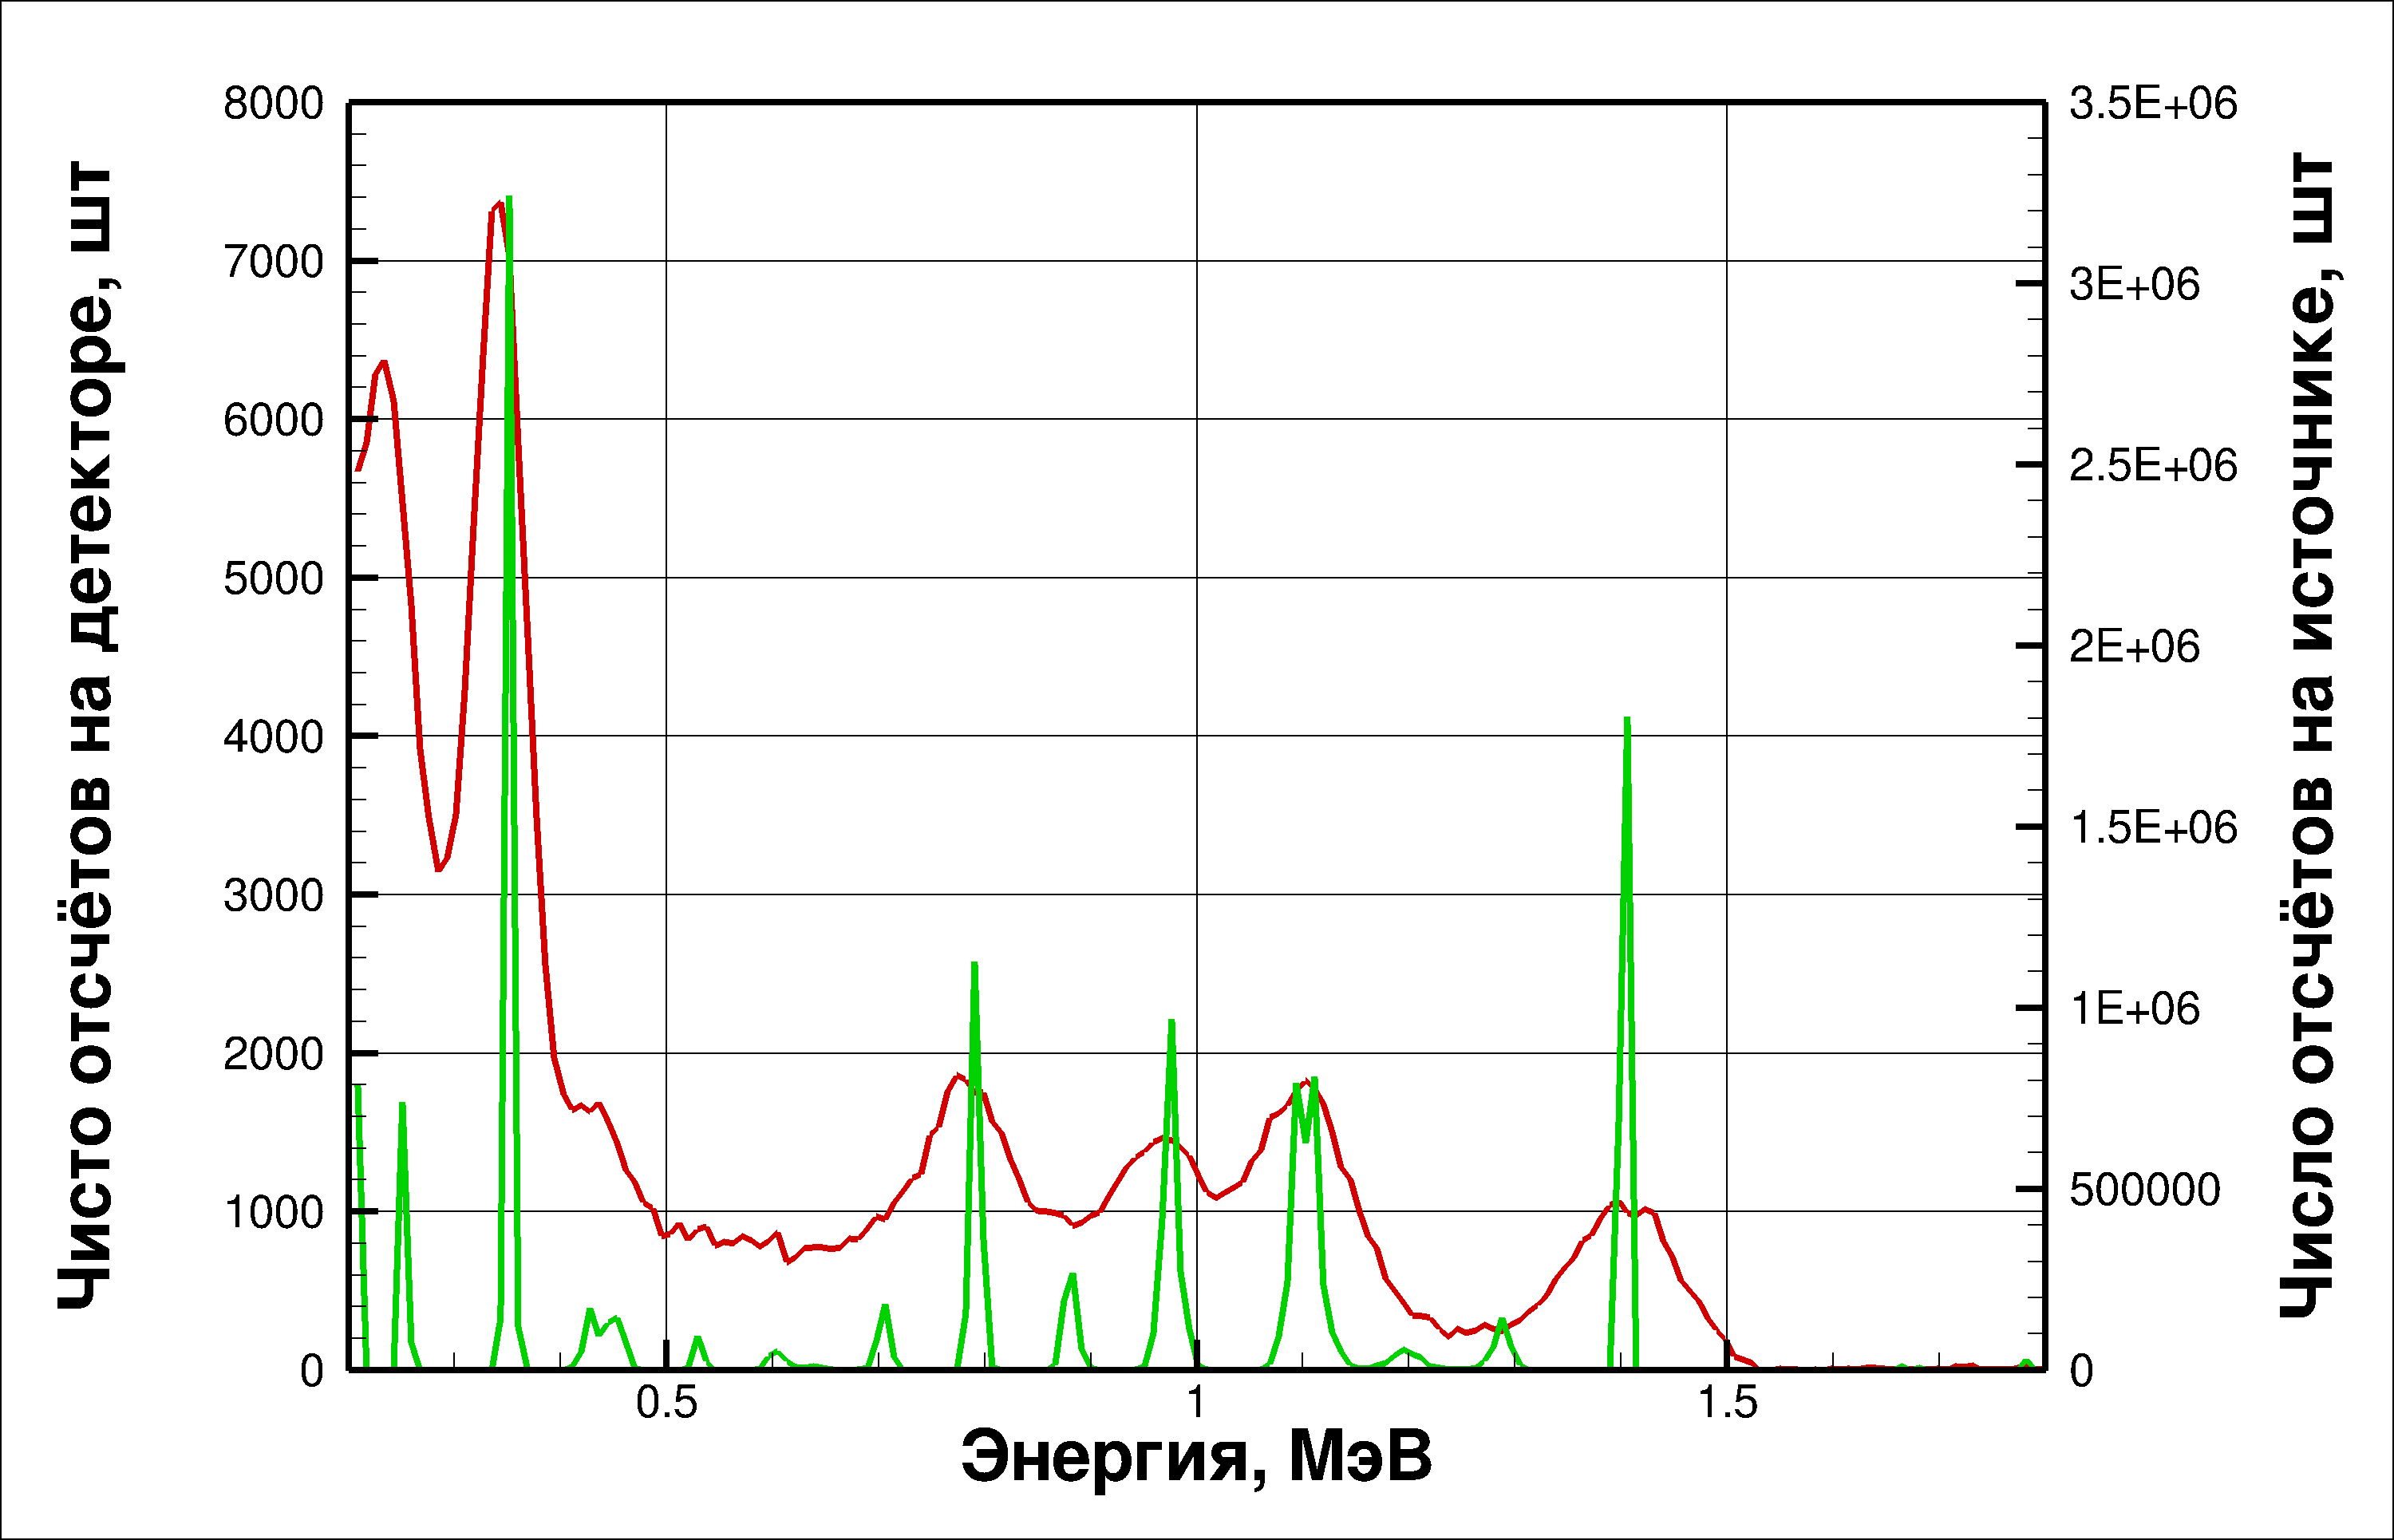
\includegraphics[width=0.52\linewidth]{euReconstructedSpectrum} }
  \caption{ Восстановленный спектр излучения источника ${}^{152}$Eu после вычитания фона. Время набора спектра --- 300 секунд. Красная линия --- измеренный спектр (отсчёты по левой оси), зелёная линия --- восстановленный спектр (отсчёты по правой оси).~\cite{Khilkevitch2013} }
  \label{fig:euReconstructedSpectrum}
\end{figure}

\begin{table}[htbp]
    \centering
    \begin{threeparttable}
      \caption{ Интенсивности и энергии пиков восстановленного спектра источника ${}^{152}$Eu. Интенсивность линий из паспорта представляет собой сумму линий с большой интенсивностью и рядом находящихся линий малой интенсивности (менее 1\%).~\cite{Khilkevitch2013} }
        \label{tab:euReconstructedLines}
        \begin{tabular}{| p{1cm} | p{3.5cm} | p{3.5cm} | p{3.5cm} | p{3.5cm} | }
            \hline
            \makecell{\textnumero} & \makecell{ Энергия линий \\ по паспорту, \\ МэВ } & \makecell{ Энергия \\ восстановлен-\\ных линий, МэВ } & 
                \makecell{Интенсивность \\ по паспорту, c${}^{-1}$} & \makecell{Восстанов-\\ленная \\ интенсив-\\ность, c${}^{-1}$ } \\
            \hline
             1 & 0.245 & 0.243 & 3018 & 2722 \\
             2 & 0.344 & 0.349 & 11115 & 11683 \\
             3 & 0.411 & 0.428 & 945 & 994 \\
             4 & 0.444 & 0.453 & 1269 & 1300 \\
             5 & 0.563 & 0.529 & 447 & 411 \\
             6 & 0.586 & 0.604 & 367 & 441 \\
             7 & 0.688 & 0.706 & 863 & 1033 \\
             8 & 0.778 & 0.790 & 5585 & 5529 \\
             9 & 0.867 & 0.883 & 1841 & 1800 \\
             10 & 0.964 & 0.975 & 6229 & 6316 \\
             11 & 1.085 & 1.035 & 4815 & 4392 \\
             12 & 1.112 & 1.111 & 5501 & 5326 \\
             13 & 1.212 & 1.195 & 673 & 653 \\
             14 & 1.299 & 1.288 & 710 & 1083 \\
             15 & 1.408 & 1.406 & 8469 & 8257 \\
            \hline
        \end{tabular}
    \end{threeparttable}
\end{table}

% ==========================================================

\FloatBarrier
\section{ Восстановление функции распределения убегающих электронов по измеренному спектру излучения }

\subsection{ Использование метода ML-EM для восстановления функции распределения убегающих электронов }
\label{sec:runawayReconstructionMlem}

При торможении электрон испускает поток квантов жёсткого рентгеновского излучения, которое может быть зарегистрировано гамма детекторов. Спектр рентгеновского излучения имеет почти непрерывный характер; максимальная энергия рождённых квантов равна кинетической энергии электрона, однако вероятность рождения единственного кванта с максимальной энергией не велика, большая часть спектра излучения приходится на меньшие энергии.~\cite{Kuznetsov1974}

Спектр рентгеновского излучения, генерируемый в процессе торможения электронов, может быть описан следующей формулой:
\begin{equation}
  \label{eq:RunawayConvolution}
  g( \varepsilon ) = \int \limits_0^{ \varepsilon } f(\varepsilon') k( \varepsilon, \varepsilon' ) d \varepsilon'
\end{equation}
где $f(\varepsilon)$ --- функция распределения электронов по энергии, $k( \varepsilon, \varepsilon' )$ --- функция генерации излучения убегающими электронами. Для моноэнергетического пучка электронов с энергией $\varepsilon_0$ и интенсивностью $I$, то есть $ f(\varepsilon) = I \cdot \delta( \varepsilon - \varepsilon_0 ) $, спектр тормозного рентгеновского излучения будет равен $g(\varepsilon) = I \cdot k( \varepsilon, \varepsilon_0 )$. Очевидно что при всех значениях $\varepsilon > \varepsilon'$ значения $k( \varepsilon, \varepsilon' ) = 0$, поскольку электрон не в состоянии сгенерировать гамма квант с энергией больше, чем энергия электрона.~\cite{Shevelev2013} 

Функция $k( \varepsilon, \varepsilon' )$ может быть рассчитана с помощью кода MCNP. Она зависит от угла между линией наблюдения и угловым распределением направления движения электронов, а так же от материала, на котором происходит торможение. Интенсивность излучения оказывается пропорциональна квадрату заряда ядер, на которых происходит рассеяние, а диаграмма углового распределения излучения имеет явно выраженную анизотропию в направлении налетающего пучка электронов.~\cite{Shevelev2013}

Уравнение~\ref{eq:RunawayConvolution} можно подставить в~\ref{eq:BaseConvolution}, тогда:
\begin{equation}
  \label{eq:RunawayBaseConvolution}
  \begin{alignedat}{1}
    s( \varepsilon ) = & \int \limits_0^{+\infty} d \varepsilon' h( \varepsilon, \varepsilon' ) \int \limits_0^{\varepsilon'} d \varepsilon'' f( \varepsilon'') k( \varepsilon', \varepsilon'' ) + n(\varepsilon) \\
    = & \int \limits_0^{+\infty} d \varepsilon'' f( \varepsilon'' ) \int \limits_0^{+\infty} d \varepsilon' h( \varepsilon, \varepsilon' ) k( \varepsilon', \varepsilon'' ) + n(\varepsilon) \\ 
    = & \int \limits_0^{+\infty} d \varepsilon'' f( \varepsilon'' ) h^{tot}( \varepsilon, \varepsilon'' ) + n(\varepsilon)
  \end{alignedat}  
\end{equation}
где $h^{tot}( \varepsilon, \varepsilon'' )$ --- свёртка функций отклика из уравнения~\ref{eq:RunawayConvolution} с передаточной функцией из уравнения~\ref{eq:BaseConvolution}. Вид этого уравнения полностью совпадает с видом уравнения~\ref{eq:BaseConvolution}, и далее для решения уравнения~\ref{eq:RunawayBaseConvolution} можно применять описанный выше метод ML-EM. В связи с характером искомого решения нецелесообразно использовать возведение в степень для вытягивания пиков (уравнение~\ref{eq:BoostMlemDisturb}), но целесообразно чаще применять процедуру сглаживания. Ошибку восстановления функции распределеня можно проводить описанным выше методом Монте-Карло.~\cite{Shevelev2013}

% ----------------------------------------------------------

\subsection{Определение максимальной энергии убегающих электронов}

По итогам восстановления функции распределения обычно имеет ненулевое значение во всём диапазоне энергий; однако в тех диапазонах энергий, где функция электронов фактически равна нулю, значение вычисленной восстановленной функции распределения оказывается близка к нулю с точностью до машинной погрешности, то есть на 10--14 порядков меньше, чем значение функции распределения в её максимуме. Поскольку в правой части функции распределения наблюдается спад значений функции к ненулевому значению, встаёт вопрос о том, какую именно энергию выбирать в качестве максимальной энергии убегающих электронов. Очевидно, что фактически такая энергия имеет физический смысл согласно уравнению~\ref{eq:MaxRunawayEnergyLimit} (в отличие например от максвелловского распределения, где понятие максимальной энергии не имеет строгого физического смысла). 

Предлагается для поиска максимальной энергии найти такое значение $\varepsilon_{max}$, что
\begin{equation}
  \label{eq:RunawayMaxEnergy}
  \rho = 1 - \frac{ \int \limits_{\varepsilon_0}^{\varepsilon_{max}} f(\varepsilon) d\varepsilon }{ \int \limits_{\varepsilon_0}^{+\infty} f(\varepsilon) d\varepsilon }
\end{equation}
где значение $\rho$ --- параметр, равный например $10^{-3}$. Значение начальной энергии интегрирования $\varepsilon_0$ ненулвевое, потому что в некоторых ситуациях функция распределения убегающих электронов очень сильно возрастает вблизи нуля, что приводит к сильной зависимости результата вычисления от порога. Обычно значение $\varepsilon_0$ имеет смысл выбирать в районе 1--2~МэВ. По физическому смыслу формулы~\ref{eq:RunawayMaxEnergy} больше выбранной максимальной энергии $\varepsilon_{max}$ на функции распределения находится статистически незначительное число электронов. Как показывает практика, значение $\varepsilon_{max}$ очень слабо зависит от произвольно выбираемых параметров $\rho$ и $\varepsilon_0$, поскольку обычно правый край полученной функции распределения имеет крутой правый край. Крутизна этого края определяется как физическими процессами, так и является следствием применения процедуры сглаживания, которая применяется при восстановлении функции распределения.~\cite{Shevelev2017}

% ----------------------------------------------------------

\subsection{ Проверка корректности восстановления и отработка методики восстановления функции распределения убегающих электронов по энергии на модельных спектрах }

Если для тестирования процедуры восстановления дискретного спектра можно использовать калибровочные источники гамма излучения, то для тестирования восстановления функции распределения убегающих электронов подобный удобный тестовый объект с известным распределением в нашем распоряжении отсутствует. Поэтому для проверки были использованы сгенерированные и обработаны модельные сигналы.

Для тестирования с помощью кода MCNP с учетом положения детектора NaI(Tl) в Roof lab с вертикальной линией обзора на токамаке JET были рассчитаны спектры тормозного излучения, соответствующие потокам жёсткого рентгена от моноэнергетических электронов в средней плоскости вакуумной камеры. Некоторые из этих спектров показаны на рисунке~\ref{fig:mcnpRunawayResponseJetSh2013}. В модели пучок ускоренных электронов с заданным распределением энергии в экваториальной плоскости корпуса JET взаимодействует с объемными ионами. Расчеты проводились в геометрии вакуумной камеры токамака JET для дейтериевой плазмы с плотностью электронов $ 5 \cdot 10^{19}$~м${}^{-3}$ и 2\% примеси углерода. Расчёты выполнены А.~Шевелевым.~\cite{Shevelev2013} 

\begin{figure}[ht!]
  \centerfloat{ 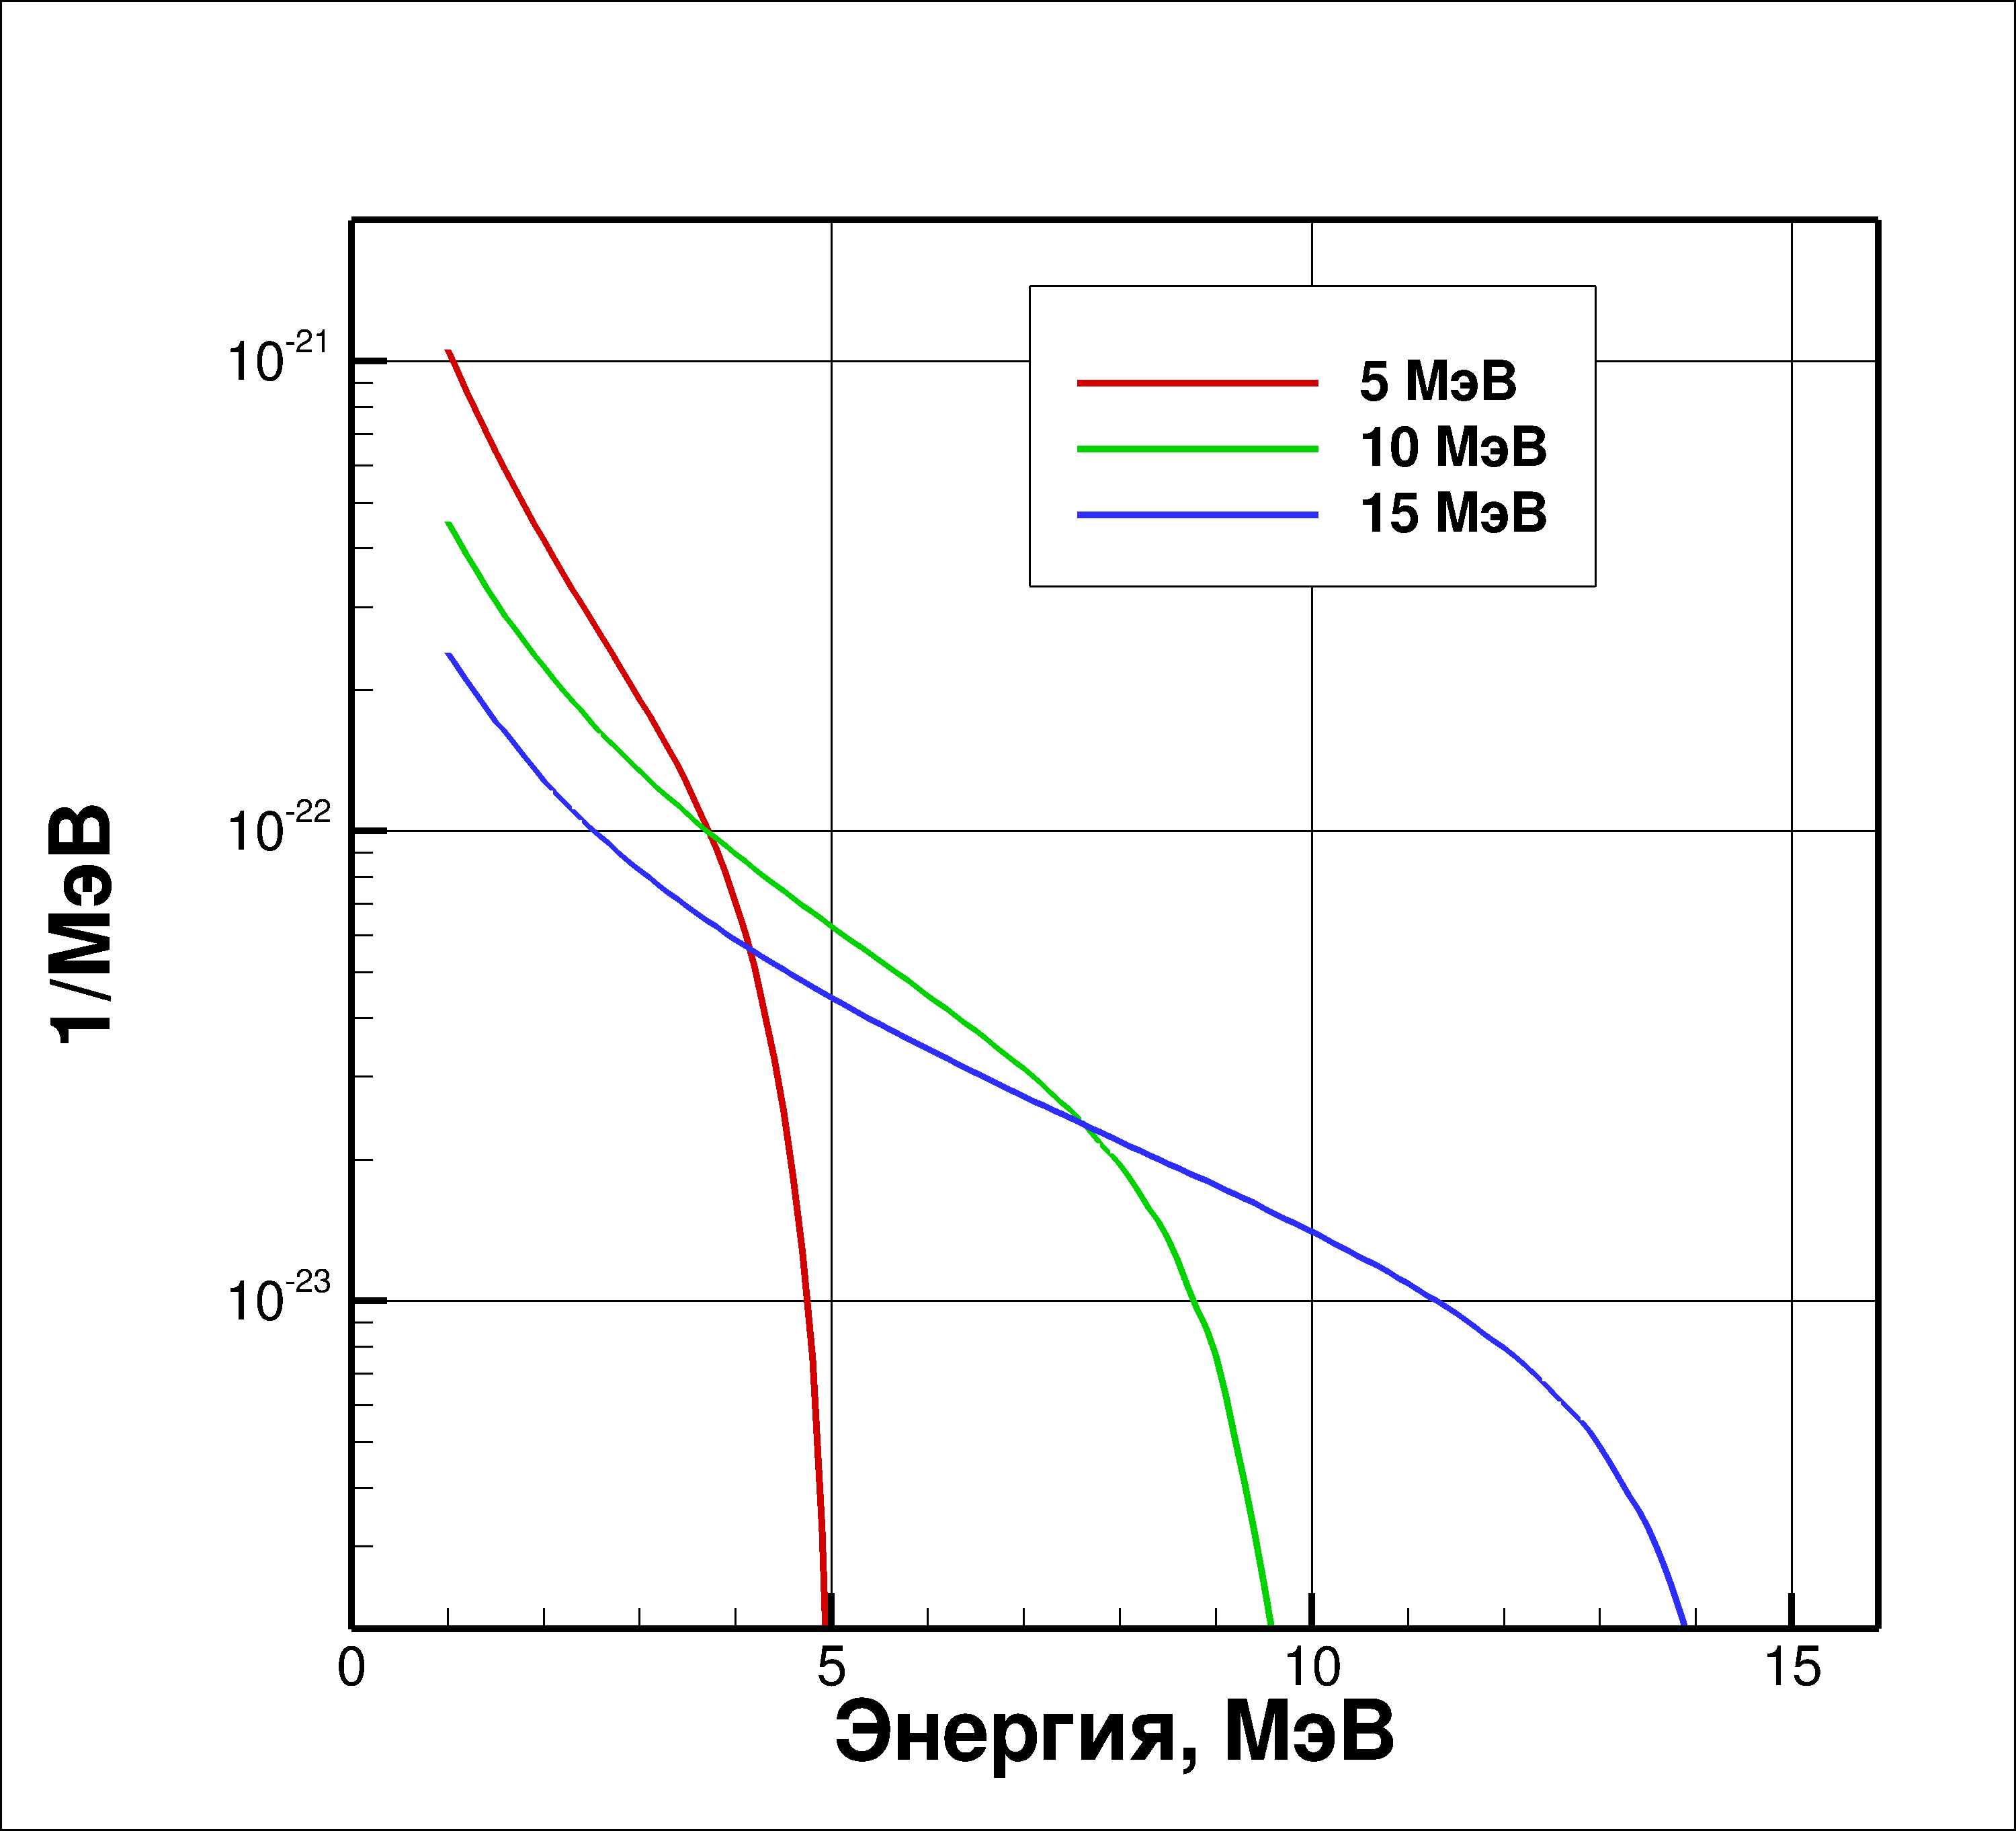
\includegraphics[width=0.52\linewidth]{mcnpRunawayResponseJetSh2013} }
  \caption{ Спектры жёсткого рентгеновского излучения, генерируемые убегающими электронами с энергиями 5, 10, 15~МэВ, рассчитанные с помощью кода MCNP. Расчёт проведён для условий токамака JET.~\cite{Shevelev2013} }
  \label{fig:mcnpRunawayResponseJetSh2013}
\end{figure}

Распределение энергии электронов, используемое в моделировании, показано на рисунке~\ref{fig:runawayJetSimulationEdfSh2013} зеленой линией с широким пиком в области высоких энергий. Такая форма распределения вполне реальна при наличии первичных и вторичных механизмов генерации убегающих электронов, а также в условиях, ограничивающих неуправляемый рост энергии, например, за счет потерь на синхротронное излучение~\cite{MartinSolis1999,Shevelev2013}. Интеграл по  распределению равен числу электронов, прошедших через видимый объем плазмы. По этой функции распределения с использованием функции генерации, изображённой на рисунке~\ref{fig:mcnpRunawayResponseJetSh2013} и с использованием функции, изображённой на рисунке~\ref{fig:mcnpInstFunctionsNaI} был построен спектр жёсткого рентгеновского излучения, который регистрируется детектором. Этот спектр изображён зелёными точками на рисунке~\ref{fig:runawayJetSimulationSpectrumSh2013}. На спектр был наложен шум, соответствующий пуассновской статистике.~\cite{Shevelev2013}

\begin{figure}[ht!]
  \centerfloat{ 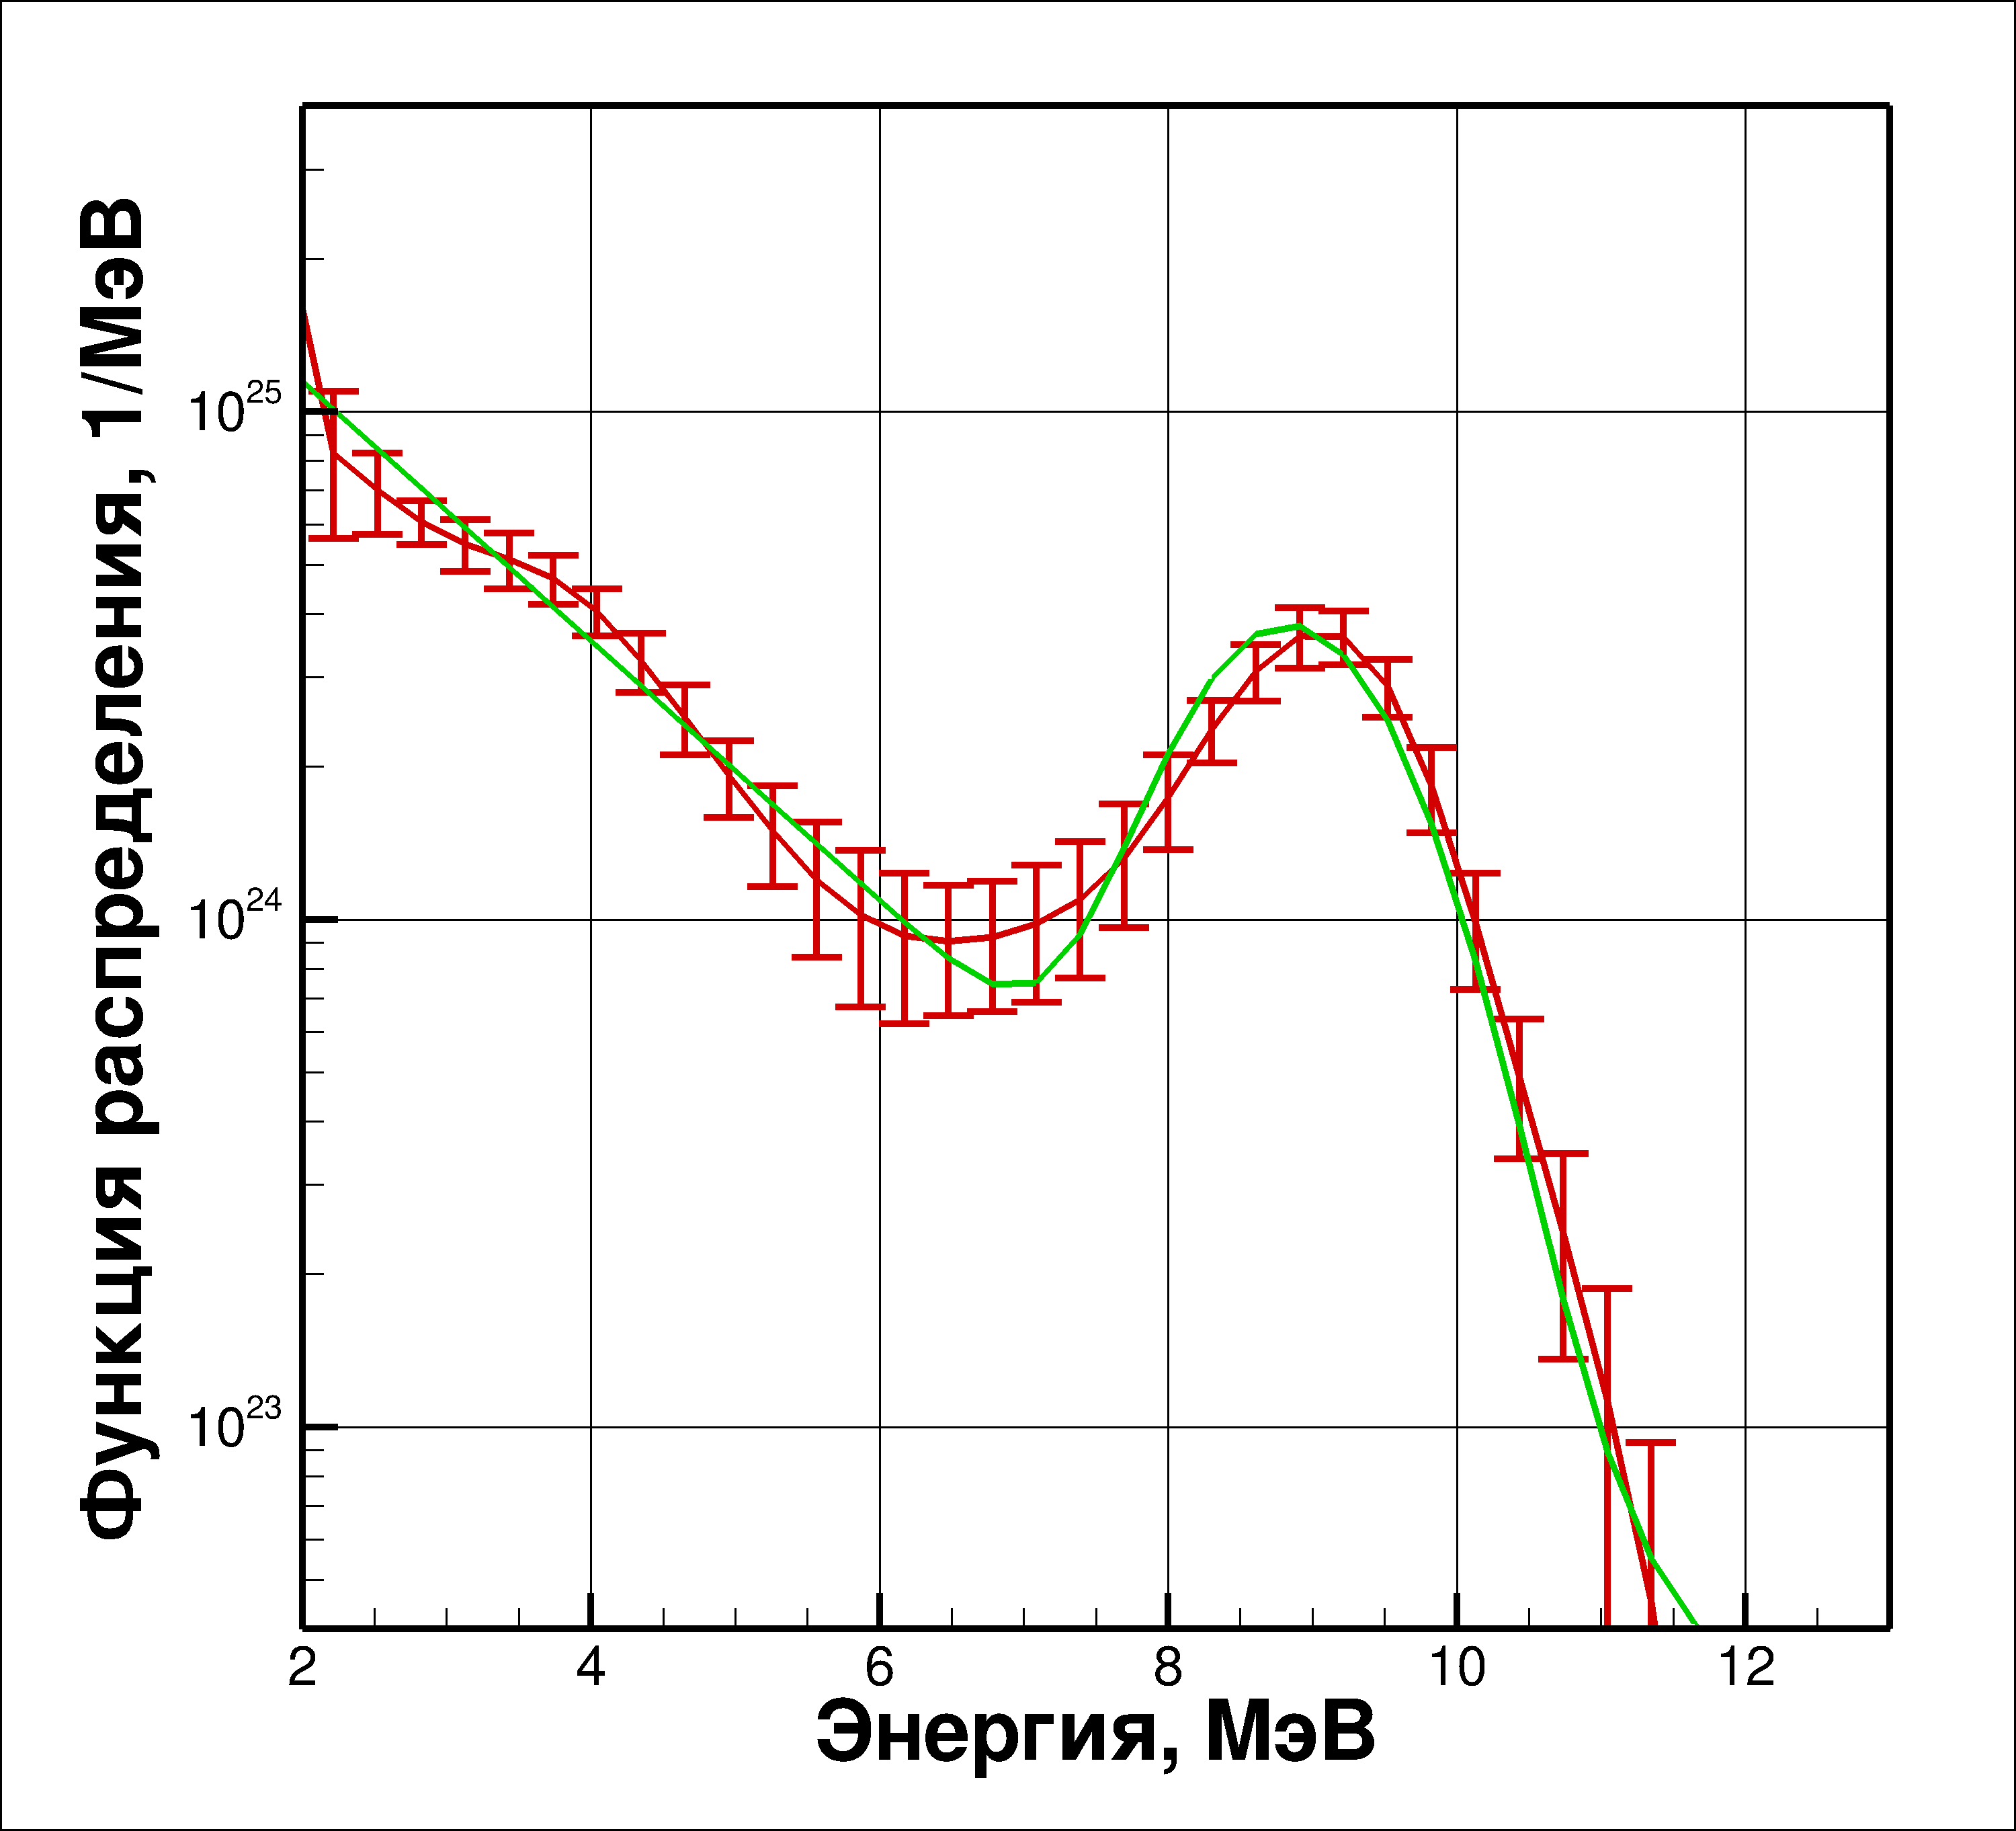
\includegraphics[width=0.52\linewidth]{runawayJetSimulationEdfSh2013} }
  \caption{ Функции распределения убегающих электронов: зелёным цветом показана сгеренированая функция распределения, красным --- восстановленная.~\cite{Shevelev2013} }
  \label{fig:runawayJetSimulationEdfSh2013}
\end{figure}

\begin{figure}[ht!]
  \centerfloat{ 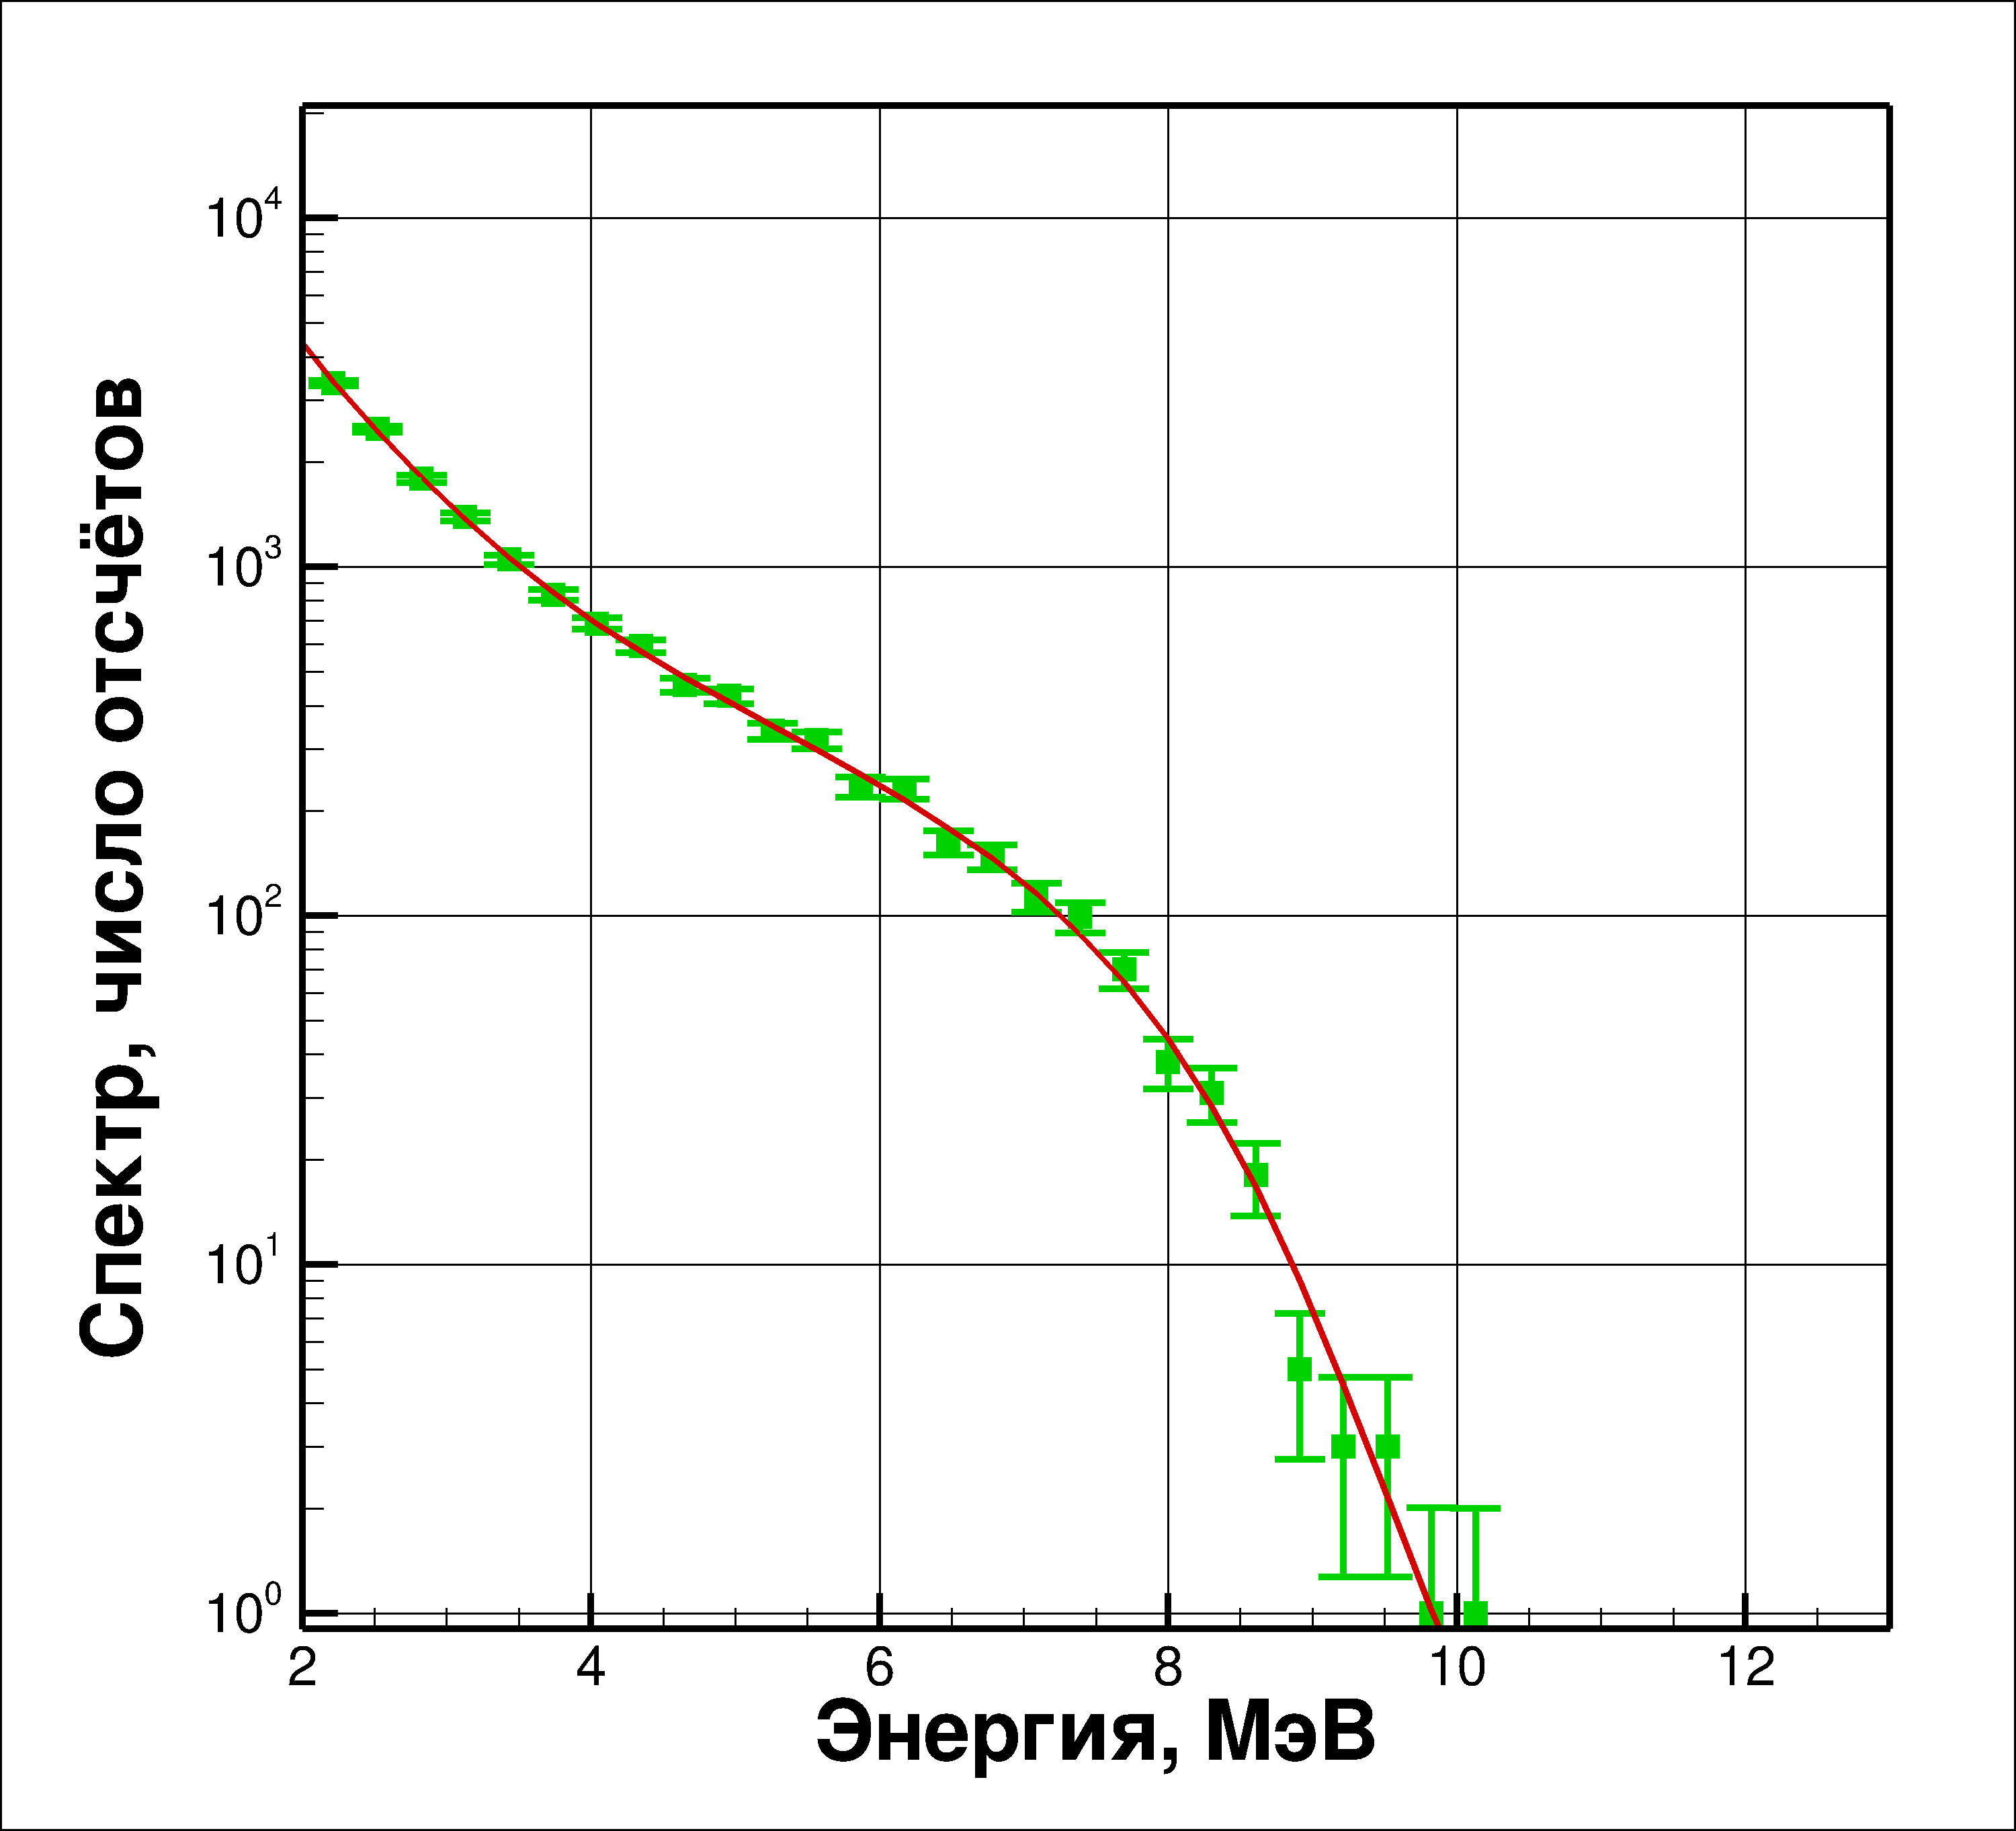
\includegraphics[width=0.52\linewidth]{runawayJetSimulationSpectrumSh2013} }
  \caption{ Спектр жёсткого рентгеновского излучения: зелёным цветом показан спектр, соответствующий сгенерированной функции распределения с рисунка~\ref{fig:runawayJetSimulationEdfSh2013}, полученный по формуле~\ref{eq:RunawayBaseConvolution}, красным цветом показан спектр, соответствующий восстановленной функции распределения с того же рисунка.~\cite{Shevelev2013} }
  \label{fig:runawayJetSimulationSpectrumSh2013}
\end{figure}

К сгеренрированному спектру была применена описанная в разделе~\ref{sec:runawayReconstructionMlem} процедура восстановления функции распределения убегающих электронов по энергии. Результат восстановления показан на рисунке~\ref{fig:runawayJetSimulationEdfSh2013} красным цветом. Восстановленное распределение электронов продемонстрировало очень близкое совпадение с модельным спектром и дало максимальную энергию 11~МэВ с очень высокой точностью. Отметим, что самые высокоэнергетичные отсчёты на спектре рентгеновского излучения не превышают значения по энергии в 10~МэВ. Причиной этого является ограниченная статистика регистрируемого спектра излучения: если бы спектр набирался бесконечно большое время, то и наиболее высокоэнергетичные кванты соответствовали бы максимальной энергии убегающих электронов. Однако поскольку убегающий электрон с энергией $\varepsilon$ с очень маленькой вероятностью генерирует квант с той же энергией $\varepsilon$, то при ограниченной статистике спектра с высокой вероятностью ни один из таких квантов не будет зарегистрирован, будут регистрироваться только кванты с меньшей энергией. Алгоритм восстановления использует информацию из всего спектра, тем самым он позволяет восстановить функцию распределения электронов для всей энергетической области.~\cite{Shevelev2013}

% ----------------------------------------------------------

\subsection{ Проверка корректности восстановления и отработка методики восстановления функции распределения убегающих электронов по энергии с помощью экспериментальных данных }

Не смотря на отсутствие подходящего контролируемого источника убегающих электронов с известным распределением, можно провесит косвенную проверку корректности процедуры восстановления функции распределения. Для этого были использованы результаты, полученные в ходе эксперимента на токамаке Туман-3М. На этом токамаке были установлены два гамма-спектрометра NaI(Tl) $\varnothing$70$\times$70~мм, направленные на лимиттер под разными углами. Принципиальная схема экспериментальной установки показана на рисунке~\ref{fig:tumanHxdDetectors}. Детектор~1 имеет направление обзора, противоположное направлению движения убегающих электронов по токамаку, а направление обзора детектора~2 наоборот совпадает с направлением их движения. Для обоих детекторов А.~Шевелевым рассчитаны функции отклика на тормозное излучение, вызванное торможением на лимиттере быстрыми электронами, в диапазоне энергий 0.1--15~МэВ. 

\begin{figure}[ht!]
  \centerfloat{ 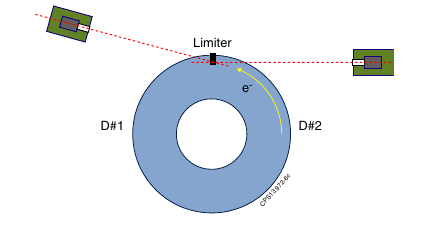
\includegraphics[width=0.72\linewidth]{tumanHxdDetectors} }
  \caption{ Расположение детекторов NaI(Tl) на токамаке Туман-3М.~\cite{Shevelev2013} }
  \label{fig:tumanHxdDetectors}
\end{figure}

Спектры жёсткого рентгеновского излучения, зарегистрированные детекторами 1 и 2 в процессе нарастания тока плазмы Туман-3М в разреженном (плотность $2-3 \times 10^{19}$~м${}^{-3}$) разряде, показаны на рисунках~\ref{fig:tumanHxdSpectrumsEdf}, (a) и (b) чёрными точками. Оба спектра наблюдают одно и то же место на лимиттере, различие в спектрах обусловлено различием в направлении наблюдения. Затем из спектра, измеренного детектором~1, была восстановлена функция распределения электронов по энергии. Она показана на рисунке~\ref{fig:tumanHxdSpectrumsEdf} (c). При восстановлении никак не использовалась информация с детектора~2. По полученной таким образом функции распределения были обратно рассчитаны спектры жёсткого рентгена для детекторов 1 и 2, которые показаны рисунках~\ref{fig:tumanHxdSpectrumsEdf}, (a) и (b) синими линиями. Видно, что рассчитанные таким образом спектры очень близки к экспериментальным. Для детектора~1 такое совпадение ожидаемо, поскольку для получения функции распределения использовался спектр с этого детектора в качестве исходных данных. Информация с детектора~2 не использовалась при получении функции распределения, однако и для него видно очень хорошее совпадение экспериментального и вычисленного спектров. Это может свидетельствовать о корректности всей процедуры --- как расчёта аппаратных функций и функций генерации излучения, так и собственно процедуры восстановления.~\cite{Shevelev2013}

\begin{figure}[ht!]
  \centerfloat{ 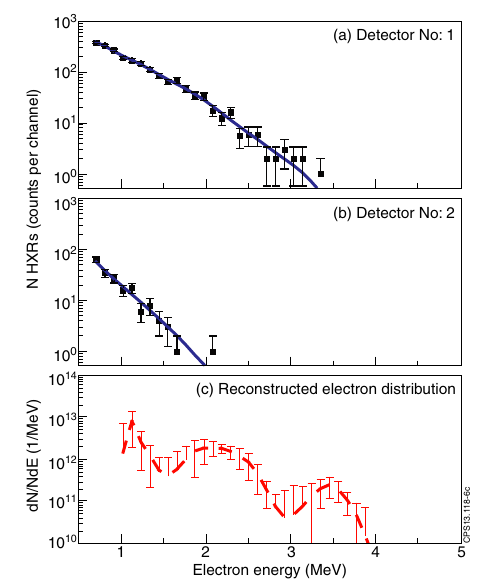
\includegraphics[width=0.52\linewidth]{tumanHxdSpectrumsEdf} }
  \caption{ a --- спектр, измеренный с помощью детектора~1; b --- спектр, измеренный с помощью детектора~2; c --- восстановленная функция распределения убегающих электронов по энергии. На рисунках (a) и (b) чёрными точками показан измеренный спектр, синий линией --- спектр излучения, соответствующий функции распределения, изображённой на рисунке (c).~\cite{Shevelev2013} }
  \label{fig:tumanHxdSpectrumsEdf}
\end{figure}

Стоит отметить, что было бы интересно восстановить функцию распределения убегающих электронов независимо с детекторов 1 и 2, и сравнивать уже сами функции распределения. Однако для более-менее корректного восстановления требуется достаточная статистика измеренных спектров. Для используемых на токамаке Туман-3М детекторов NaI(Tl) почти невозможно получить хорошую статистику на обоих детекторах: или на одном из детекторов она будет достаточно хорошей, а на другом --- недостаточной, или на втором она будет достаточной, но тогда загрузка первого детектора окажется чрезвычайно большой, и построить спектр окажется практически невозможно. 

% ----------------------------------------------------------

\subsection{ Влияние статистики и загрузки детектора на результаты восстановления функции распределения }

Очевидно что точность восстановления функции распределения будет зависеть от статистики измеренного спектра. На рисунке~\ref{fig:ft2TestReStatistics} представлены смоделированные спектры жесткого рентгеновского излучения. Исходная модельная функция распределения имела колокообразный профиль с максимальной энергией 8~МэВ, показанный на правых рисунках (d)--(f) красными линиями. Использовались функции отклика детектора LaBr3(Ce) $\varnothing$25.4$\times$76.2~мм, с помощью которого проводились измерения на токамаке ФТ-2; они показаны на рисунке~\ref{fig:ft2HxrDetectrorsAndReResponse}~(а). Были использованы функции генерации излучения убегающими электронами, соответствующие условиям токамака ФТ-2; они показаны на рисунке~\ref{fig:ft2HxrDetectrorsAndReResponse}~(б). После вычисления спектра на него был наложен пуассоновский шум. Полный интеграл числа событий в модельном спектре составлял $10^3$, b) $10^4$ и c) $10^5$~событий. Спектры показаны на рисунке~\ref{fig:ft2TestReStatistics} (a)--(c) чёрными точками.~\cite{Shevelev2016}

\begin{figure}[ht!]
    \begin{minipage}[b][][b]{0.45\linewidth}\centering
        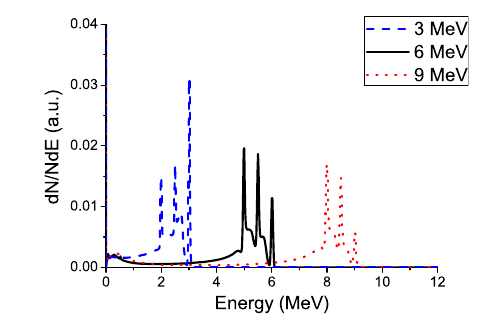
\includegraphics[width=0.92\linewidth]{ft2HxrDetectrorsResponse} \\ а) \\
    \end{minipage}
    \hfill
    \begin{minipage}[b][][b]{0.45\linewidth}\centering
        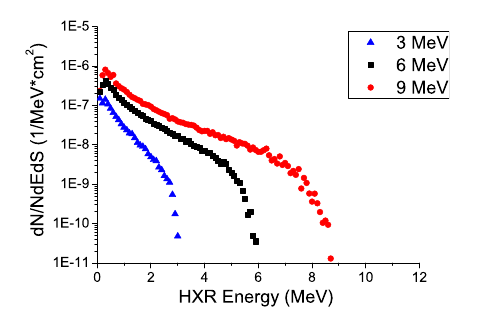
\includegraphics[width=0.92\linewidth]{ft2HxrReGenerationResponse} \\ б) \\
    \end{minipage}
    \vspace{5mm}
    \caption{ (а) --- отклик детектора LaBr3(Ce), использовавшегося в измерениях на токамаке ФТ-2, расчитанный кодом MCNP; (б) --- функции генерации тормозного жёсткого рентгеновского излучения убегающими электронами при взаимодействии с лимиттером, расчитанные кодом MCNP~\cite{Shevelev2016}. }
    \label{fig:ft2HxrDetectrorsAndReResponse}
\end{figure}

\begin{figure}[ht!]
  \centerfloat{ 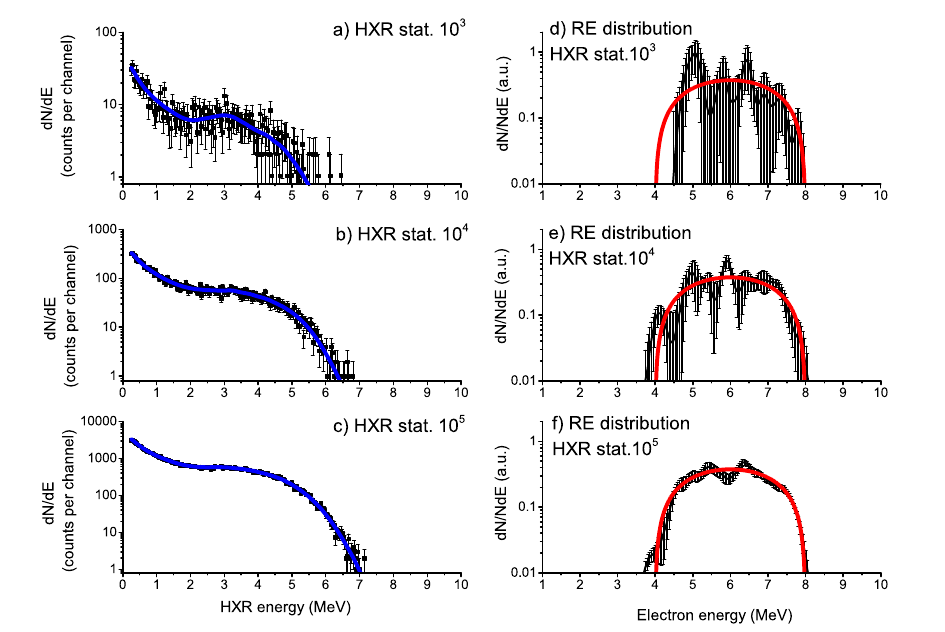
\includegraphics[width=0.95\linewidth]{ft2TestReStatistics} }
  \caption{ Левая колонка --- модельные спектры жёсткого рентгеновского излучения, сгенерированные с разной статистикой: a) $10^3$, b) $10^4$ и c) $10^5$~событий. Правая колонка --- результаты восстановления модельной функции распределения электронов для различной статистики спектров: d) $10^3$, e) $10^4$ и f) $10^5$~событий. Модельная функция распределения электронов показана красной линией, чёрная линия --- результат восстановления. На левых графиках чёрными точками показаны сгенреированные спектры, синими линиями показаны свертки полученных в результате восстановления электронных распределений с функцией отклика детектора и функцией генерации излучения.~\cite{Shevelev2016} }
  \label{fig:ft2TestReStatistics}
\end{figure}

Результат восстановления функции распределения по сгенерированным спектрам показан на рисунке~\ref{fig:ft2TestReStatistics} (d)--(f) чёрными линиями. Синие линии на левых графиках представляют собой свертки полученных распределений с функцией отклика детектора и функцией генерации излучения. На спектрах виден эффект улучшения результатов восстановления с улучшением статистики. Даже при низкой статистике в $10^3$~событий удалось корректно описать правый край функции распределения, а так же получить общую форму функции распределения. Отметим, что в экспериментах обычно статистика спектра лежит в исследуемом диапазоне $10^3$--$10^5$ событий в спектре~\cite{Shevelev2016}

Обращает на себя внимание то, что максимальная энергия зарегистрированных квантов жёсткого рентгеновского излучения оказывается всегда меньше чем максимальная энергия убегающих электронов. Разница между максимальной энергией квантов излучения и максимальной энергией электронов тем больше, чем меньше статистика спектра. Это обусловлено сильно спадающим характером функции генерации излучения убегающими электронами, который хорошо виден на рисунках~\ref{fig:mcnpRunawayResponseJetSh2013} и \ref{fig:ft2HxrDetectrorsAndReResponse}.~\cite{Shevelev2016}

%Так же отметим, что использовавшийся в старых работах метод определения максимальной энергии убегающих электронов по 

Для исследования влияния скорости счёта на процедуру восстановления функции распределения были сгенерированы модельные осциллограммы с различной загрузкой детектора. Генерация проводилась методом, описанным в разделе~\ref{sec:SignalGeneration}. Были сгенерированы осциллограммы, соответствующие разной скоростью счёта детектора ($10^5$, $10^6$, $3\times10^6$, $10^7$~с${}^{-1}$) с распределением событий по амплитуде, соответствующим исходному распределению убегающих электронов по энергии. Затем эти осциллограммы были обработаны методом фиттинга (раздел~\ref{sec:FittingProcessing}), были построены спектры, которые были обработаны в соответствии с процедурой из раздела~\ref{sec:runawayReconstructionMlem} для восстановления функции распределения убегающих электронов по энергии. Сравнение исходной сгенерированной функции распределения и восстановленной функции распределения показано на рисунке~\ref{fig:ft2TestReCountRate}.~\cite{Shevelev2016}


\begin{figure}[ht!]
  \centerfloat{ 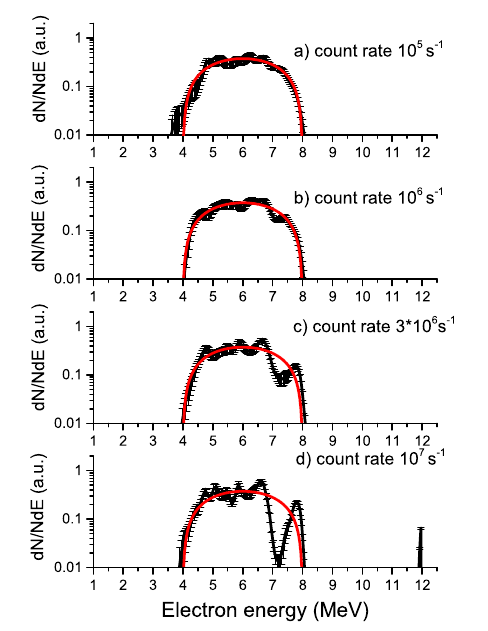
\includegraphics[width=0.95\linewidth]{ft2TestReCountRate} }
  \caption{ Восстановление функции распределения по модельным осциллограммам, соответствующим различной загрузке детектора. Красной линией показана сгенерированная осциллограмма, чёрной --- восстановленная из сгенерированного спектра.~\cite{Shevelev2016} }
  \label{fig:ft2TestReCountRate}
\end{figure}

При увеличении загрузки детектора улучшается статистика спектра и, соответственно, улучшается качество восстановления функции распределения. С другой стороны, при увеличении загрузки детектора растёт и количество наложенных импульсов на осциллограмме, что приводит к искажениям измеренного спектра (уменьшение доли низких квантов жёсткого рентгена и наоборот появлению ложных высокоэнергетичных событий). В свою очередь это приводит к аретфактам при восстановлении функции распределения. Тем не менее, отметим что максимальная энергия восстановленного распределения убегающих электронов смещается всего на 100--150~кэВ. Видно что при загрузке $10^7$~событий в секунду в области высоких энергий появлялся паразитный пик (однако число электронов в этом пике не превышает 0.5\% от общего распределения, и поэтому этот эффект следует считать пренебрежимо малым). Следует отметить, что при скорости счета детектора выше $10^7$~с${}^{-1}$ измеряемые спектры могут быть искажены из-за насыщения ФЭУ~\cite{Loher20121}, однако в моделировании этот эффект не учитывался.~\cite{Shevelev2016}

Таким образом, проведенный анализ смоделированных спектров жёсткого рентгеновского излучения с различной нагрузкой детектора и статистикой показал, что спектры, измеренные разработанным спектрометром LaBr 3(Ce) при скоростях счета до нескольких МГц, могут быть использованы для восстановления распределения энергии убегающих электронов во времени. В некоторых случаях восстановление полной функции распределения энергии убегающих электронов может привести к некоторым артефактам, которые следует тщательно анализировать. 

% ----------------------------------------------------------

\section{Выводы к главе 3}

Рассмотрено применение алгоритма ML-EM для восстановления спектра гамма излучения источников по измеренному с помощью сцинтилляционных детекторов спектру излучения. Для проведения процедуры восстановления требуется вычислить аппаратную функцию детектора и то, как ослабляется поток гамма квантов на пути от источника к детектору. Это вычисление может быть выполнено кодом MCNP. Был предложен ряд модификаций для адаптации базового алгоритма к условиям, которые имеются в задачах гамма-спектрометрии. Для вычисления погрешности восстановленного спектра предлагается использовать метод Монте-Карло.

Для проверки корректности процедуры восстановления были проведены эксперименты с калибровочными источниками ${}^{60}$Co и ${}^{137}$Cs излучения известной интенсивности. По восстановленным спектрам была рассчитана активность источников, которая совпала с точностью 1.5\% при обработке измеренного спектра с большой статистикой (время набора 300~с, расстояние до источника 25.5~см) и с точностью 2.5\% при обработке измеренного спектра с малой статистикой (время набора 2~с, расстояние до источника 25.5~см). Так же был проведён эксперимент с источником ${}^{152}$Eu, особенностью которого является наличие большого числа линий на спектре. В ходе восстановления удалось идентифицировать линии, в том числе не разрешённые на исходном измеренном спектре, и определить их интенсивность.  

Показано, что алгоритм ML-EM с модификациями применим для восстановления функции распределения убегающих электронов по энергии по измеренному спектру тормозного жёсткого рентгеновского излучения. Предложен метод определения максимальной энергии убегающих электронов по восстановленной функции распределения. 

Для проверки корректности процедуры восстановления функции распределения были проведены численные эксперименты. Было исследовано влияние статистики спектра и загрузки детектора на восстановленную функцию распределения. Показано, что при статистике спектра $10^3$ -- $10^5$~с${}^{-1}$ восстановленная функция соответствует исходной; показано, что при загрузке детектора $3 \times 10^6$~с${}^{-1}$ и выше восстановленная функция распределения оказывается искажённой из-за влияния наложений при обработке осциллограммы, однако в целом так же передаёт характер исходной функции распределения. Кроме того, для проверки процедуры восстановления были использованы результаты экспериментов на токамаке Туман-3М. В ходе этих экспериментов с помощью двух независимых детекторов измерялся спектр жёсткого рентгеновского излучения из одной и той же точки лимиттера, затем были проведены процедуры восстановления и сравнения, которые показали хорошее согласование результатов, полученных с различных независимых детекторов.

% ==========================================================

\FloatBarrier
           % Глава 3
\chapter{Диагностика убегающих электронов на токамаке Asdex Upgrade с помощью спектрометра на основе кристалла LaBr${}_3$(Ce)}\label{ch:ch5}

\FloatBarrier
           % Глава 4
\chapter{Диагоностика убегающих электронов на токамаке JET}
\label{ch:ch5}

% ==========================================================

\section{Спектрометы жёсткого рентгеновского излучения на токамаке JET}

В настоящее JET имеет самую совершенную систему гамма-спектрометрии среди действующих токамаков~\cite{Iliasova2022}. В экспериментах используются два спектрометра LaBr3(Ce) $\varnothing 76,2 \times 152,4$~мм~\cite{Nocente2010} с вертикальным и тангенциальным линиями обзора (рисунок~\ref{fig:jetHxrDetectorsScheme}, слева). Детектор с вертикальной линией обзора LaBr3(Ce) может быть заменён на один из двух других спектрометров. Первый --- HPGe-спектрометр~\cite{Tardocchi2011}, обеспечивающий высокоэффективную регистрацию гамма-излучения с исключительно высоким энергетическим разрешением (2,4~кэВ на линии 1,333~МэВ), который, однако, имеет гораздо меньшую по сравнению с LaBr3(Ce) максимальную скорость счёта. Второй --- спектрометр NaI(Tl) размером $\varnothing 5 \times 5$~дюймов, разрешение которого составляет 3\% на линии 4~МэВ~\cite{Tardocchi2008}. Спектрометр BGO с квазитангенциальной линией обзора, ранее работавший на токамаке, был заменен детектором LaBr3(Ce) ($\varnothing 76,2 \times 152,4$~мм)~\cite{Nocente2021}. В тангенциальном спектрометре полиэтиленовый аттенюатор был заменен на аттенюатор из гидрида лития (LiH)~\cite{Curuia2017}. На коллиматор вертикального спектрометра LaBr3(Ce) в дополнение к ранее существовавшему LiH-фильтру $\varnothing 30 \times 300$~мм, обогащенному изотопом ${}^6$Li, был установлен аттенюатор LiH с естественным соотношением изотопов лития длиной 400~мм~\cite{Murari2008}.

\begin{figure}[ht!]
  \centerfloat{ 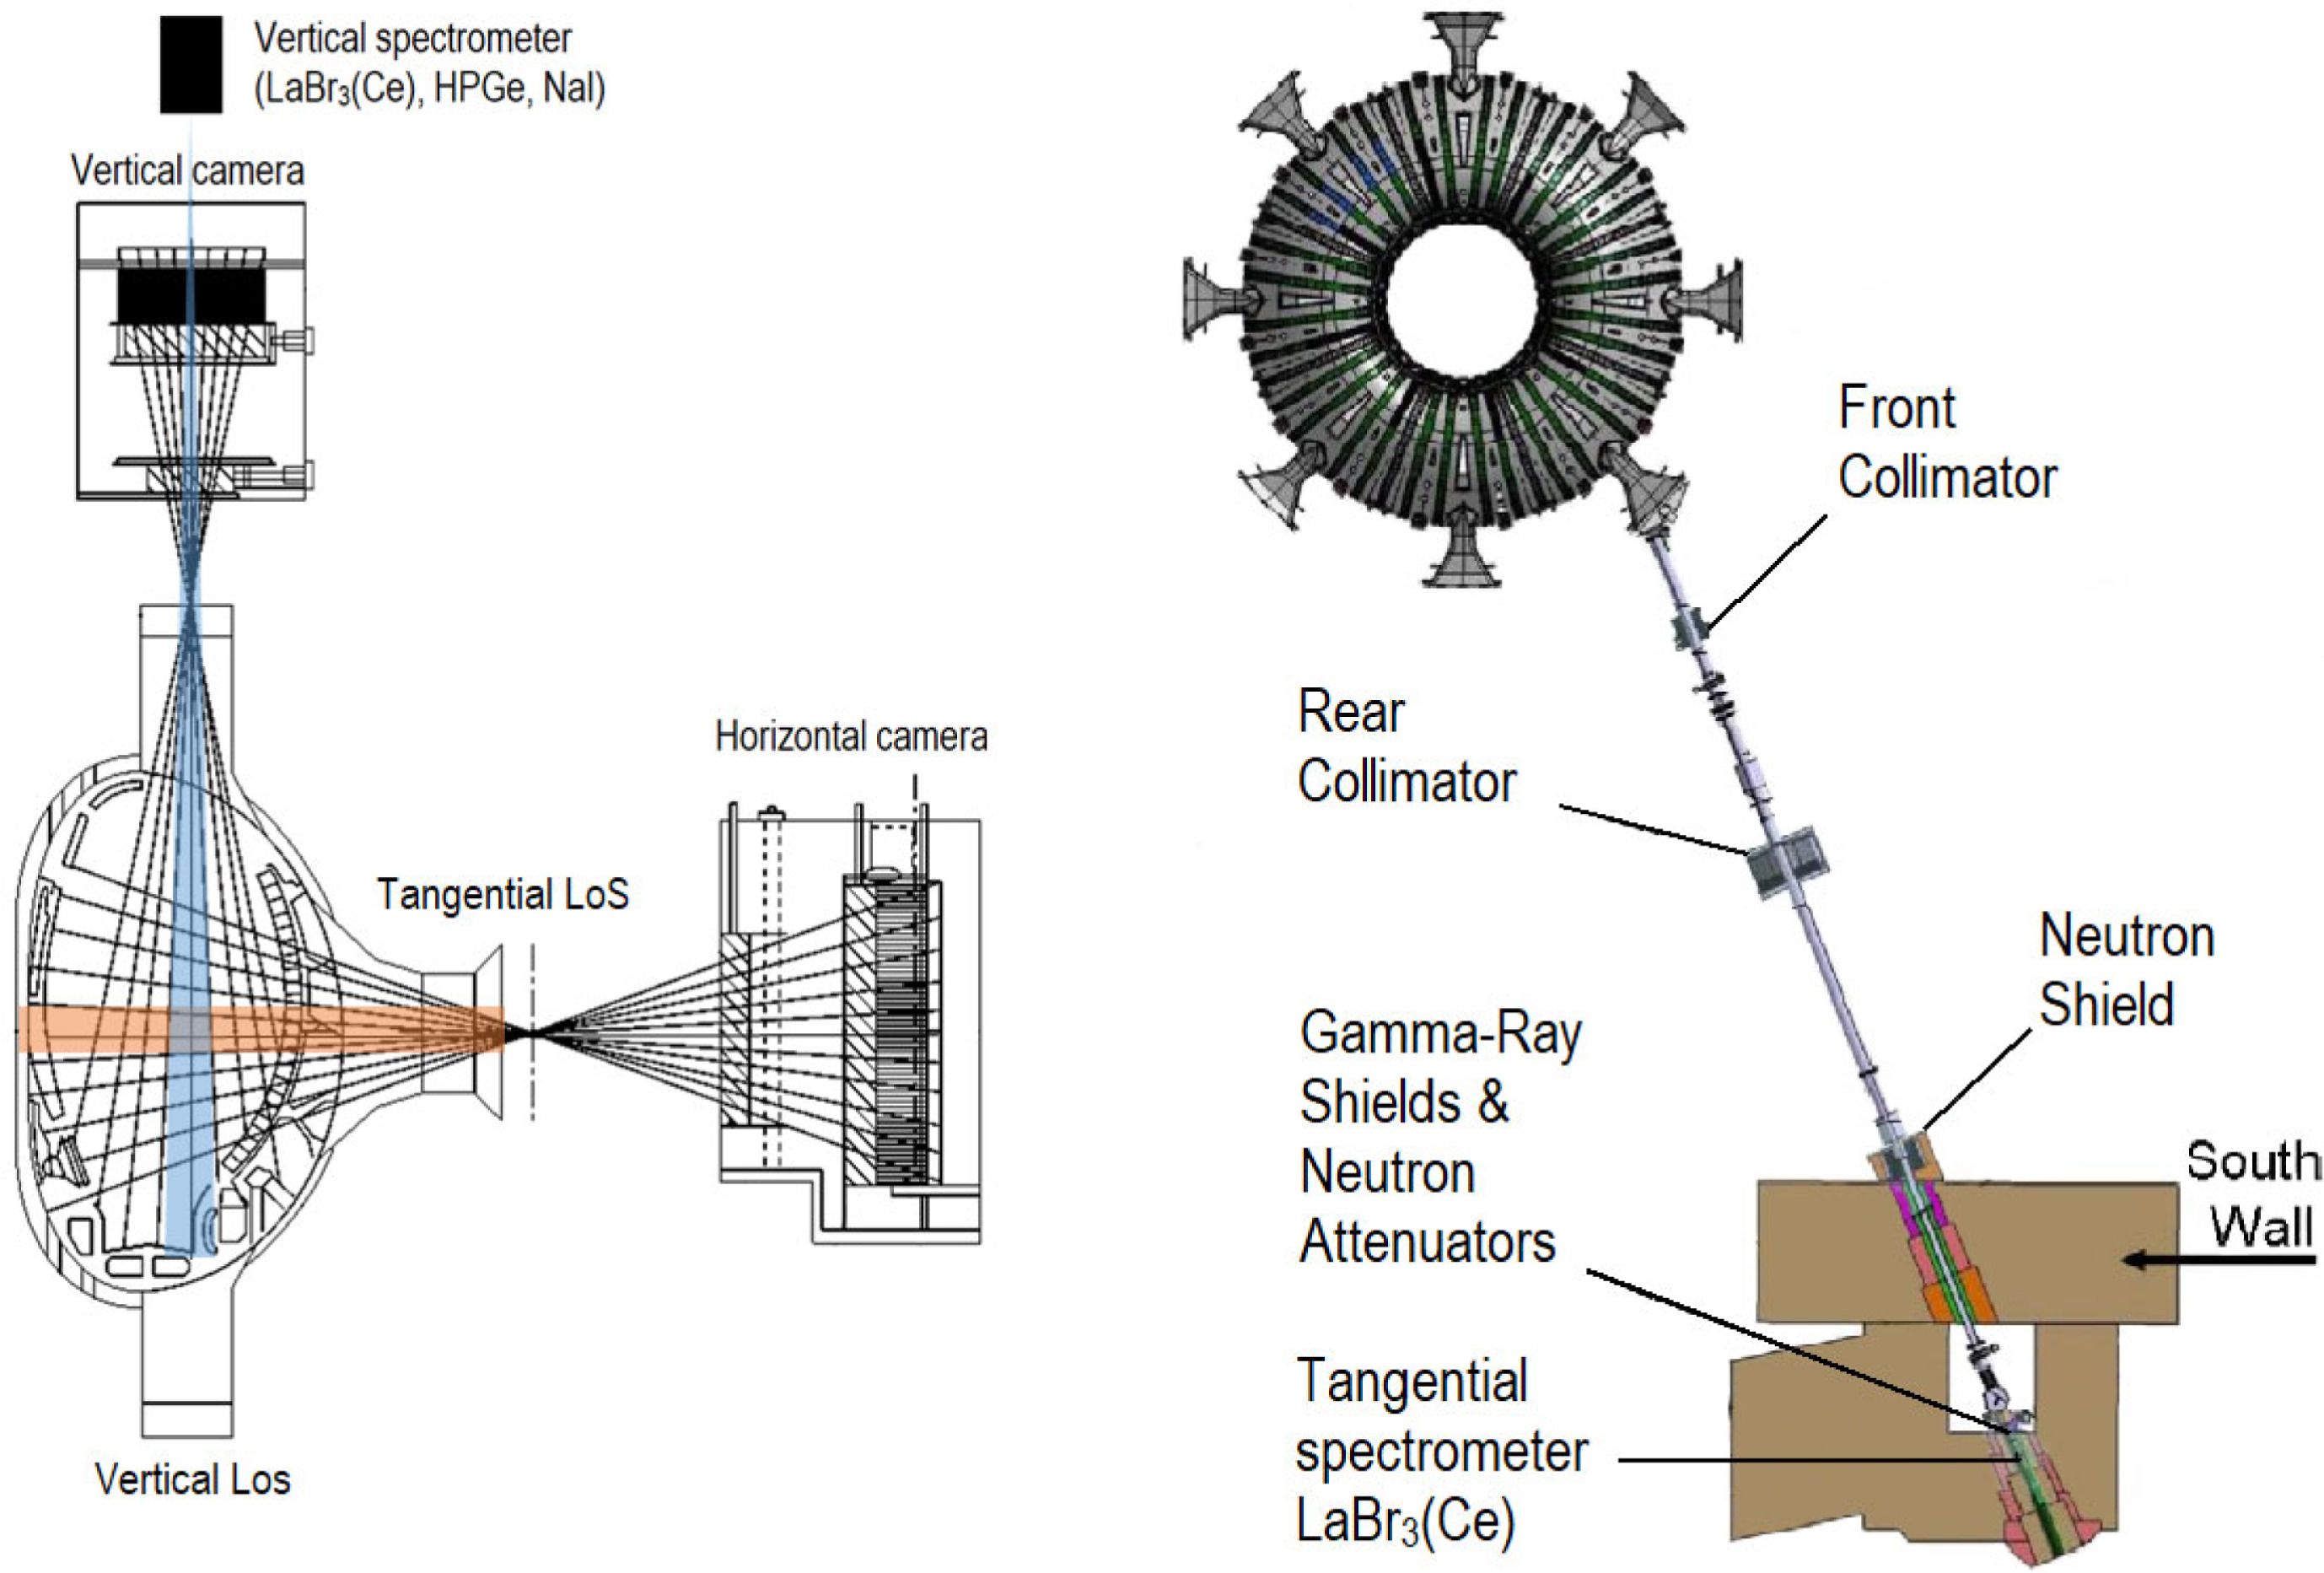
\includegraphics[width=0.92\linewidth]{jetHxrDetectorsScheme} }
  \caption{ Расположение гамма-спектрометров на токамаке JET.~\cite{Iliasova2022} }
  \label{fig:jetHxrDetectorsScheme}
\end{figure}

Сигнал со спектрометров LaBr3(Ce) записывается в сегментной моде~\cite{Pereira2008,Pereira2011} когда сохраняются только части осциллограммы, превышающие некоторый заданный порог, и их окрестности. Для оцифровки используется 14-битное АЦП с частотой 400~МГц. Сохранённые осциллограммы записываются в систему сбора и обработки данных CODAS, откуда могут быть впоследствии извлечены и обработаны, например, с помощью алгоритмов, описанных в главах~\ref{ch:ch2} и \ref{ch:ch3}. 

В дополнение к этим спектрометрам для получения двумерных измерений профилей гамма-излучения может использоваться гамма-камера, состоящая из 19~компактных детекторов с 10~горизонтальными и 9~вертикальными линиями обзора (рисунок~\ref{fig:jetHxrDetectorsScheme}, справа). Компактные детекторы изготовлены из кристаллов LaBr3(Ce) $\varnothing 25 \times 17$~мм~\cite{Rigamonti2018}. Выходной сигнал от каждого детектора оцифровывается 13-битном АЦП со скоростью 200 отсчётов в секунду~\cite{Fernandes2018}.

Все диагностики токамака JET сохраняют результаты измерений в системе CODAS~\cite{Jones1986}. Для обработки данных в компьютерный код ``DeGaSum'' была добавлена возможность загрузки данных из системы CODAS с всех вышеперечисленных гамма-диагностик. Для детекторов на основе BGO и HPGe доступны спектры, созданные в результате обработки с помощью программно-аппаратных средств диагностик. Для детекторов NaI(Tl), LaBr3(Ce) доступны осциллограммы, обработка которых с помощью продвинутых алгоритмов, описанных в главе~\ref{ch:ch2}, может позволить получить больше полезной информации. Итоговые спектры жёсткого рентгеновского излучения могут быть обработаны с помощью алгоритмов, описанных в главе~\ref{ch:ch3}. 

% ==========================================================

\section{Восстановление функции распределения убегающих электронов на токамаке JET}

Для восстановления функций распределения были предварительно рассчитаны функции отклика детектора и функции генерации убегающими электронами жёсткого рентгеновского излучения. Расчёты были выполнены А.~Е.~Шевелевым с помощью кода MCNP, примеры полученных функций показаны на рисунке~\ref{fig:jetGenerationFunctions}. 

\begin{figure}[ht!]
  \centerfloat{ 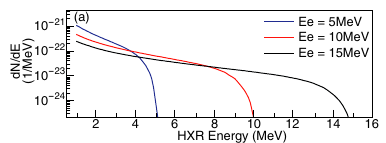
\includegraphics[width=0.85\linewidth]{jetGenerationFunctions} }
  \caption{ Спектры жёсткого рентгеновского излучения, генерируемые пучком моноэнергетических электронов с различной энергией, рассчитанные для условий токамака JET.~\cite{Shevelev2013} }
  \label{fig:jetGenerationFunctions}
\end{figure}


Разработанный код DeGaSum был использован для восстановления распределений убегающих электронов по измеренным спектрам жёсткого рентгеновского излучения на токамаке JET. Рисунок~\ref{fig:jetRunawayEdf82715} иллюстрируют применение кода DeGaSum для диагностики убегающих электронов на токамаке JET. В качестве примера можно рассмотреть разряд №~82715, в котором при нарастании тока возник пучок убегающих электронов. Спектры жёсткого рентгеновского излучения были измерены с помощью   детектором NaI(Tl) с вертикальной линией обзора, после чего были обработаны с помощью программы DeGaSum. Спектры излучения, генерируемые быстрыми электронами при взаимодействии с ионами плазмы и зарегистрированные спектрометром, показаны на верхних рисунках \ref{fig:jetRunawayEdf82715} черными точками. Восстановленные функции распределения убегающих электронов представлены красными линиями на нижних рисунках. Результаты свёрток полученных функций распределения с функциями отклика детектора показаны на рисунках синими линиями. В этом разряде генерация пучка убегающих электронов происходила при нарастании тока при малой плотности и прекращалась при увеличении плотности.~\cite{Shevelev2013} 

%\begin{figure}[ht!]
%  \centerfloat{ 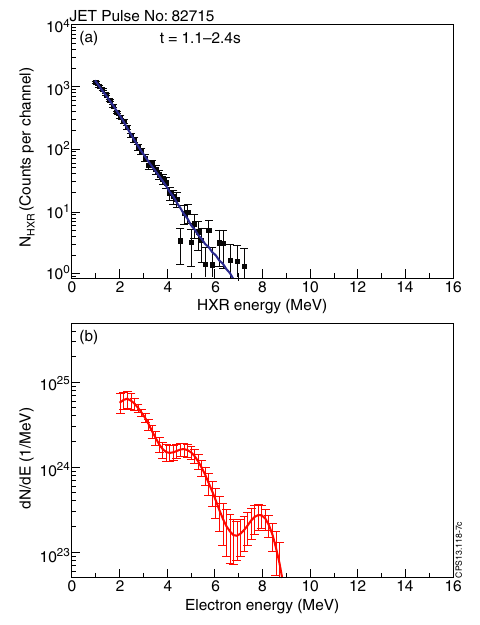
\includegraphics[width=0.55\linewidth]{jetRunawayEdf82715_t1} }
%  \caption{ (a) --- спектр жёсткого рентгеновского излучения, зарегистрированный в период 41,1--42,4 с помощью детектора NaI(Tl) в импульсе на токамаке JET №~82715 (черные точки), и спектр, полученный после свёртки восстановленной функции распределения электронов с функцией отклика детектора (синяя линия); (b) --- восстановленная функция распределения энергии убегающих электронов.~\cite{Shevelev2013} }
%  \label{fig:jetRunawayEdf82715_t1}
%\end{figure}
%
%\begin{figure}[ht!]
%  \centerfloat{ 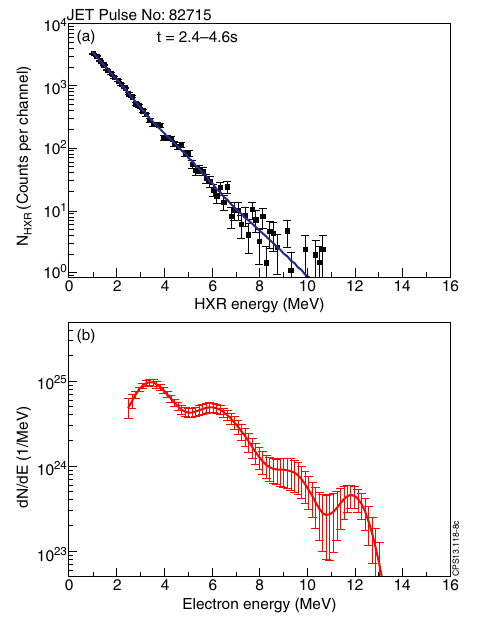
\includegraphics[width=0.55\linewidth]{jetRunawayEdf82715_t2} }
%  \caption{ (a) --- спектр жёсткого рентгеновского излучения, зарегистрированный в период 41,1--42,4 с помощью детектора NaI(Tl) в импульсе на токамаке JET №~82715 (черные точки), и спектр, полученный после свёртки восстановленной функции распределения электронов с функцией отклика детектора (синяя линия); (b) --- восстановленная функция распределения энергии убегающих электронов.~\cite{Shevelev2013} }
%  \label{fig:jetRunawayEdf82715_t2}
%\end{figure}
%
%\begin{figure}[ht!]
%  \centerfloat{ 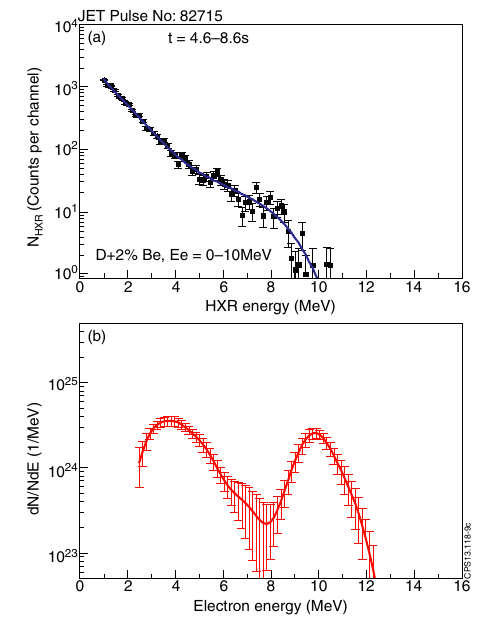
\includegraphics[width=0.55\linewidth]{jetRunawayEdf82715_t3} }
%  \caption{ (a) --- спектр жёсткого рентгеновского излучения, зарегистрированный в период 41,1--42,4 с помощью детектора NaI(Tl) в импульсе на токамаке JET №~82715 (черные точки), и спектр, полученный после свёртки восстановленной функции распределения электронов с функцией отклика детектора (синяя линия); (b) --- восстановленная функция распределения энергии убегающих электронов.~\cite{Shevelev2013} }
%  \label{fig:jetRunawayEdf82715_t3}
%\end{figure}

\begin{figure}[ht]
    \begin{minipage}[b][][b]{0.42\linewidth}\centering
        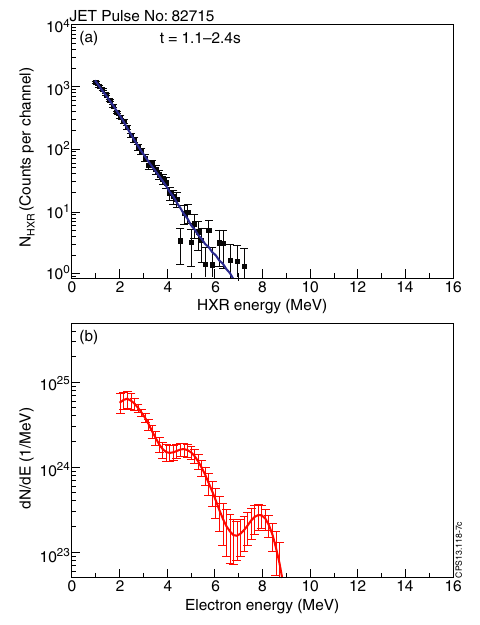
\includegraphics[width=0.98\linewidth]{jetRunawayEdf82715_t1} \\ а)
    \end{minipage}
    \hfill
    \begin{minipage}[b][][b]{0.42\linewidth}\centering
        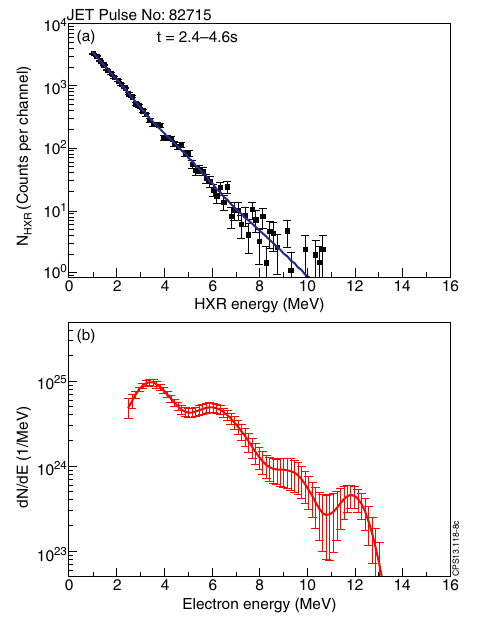
\includegraphics[width=0.98\linewidth]{jetRunawayEdf82715_t2} \\ б)
    \end{minipage}
    \hfill
    \begin{minipage}[b][][b]{0.42\linewidth}\centering
        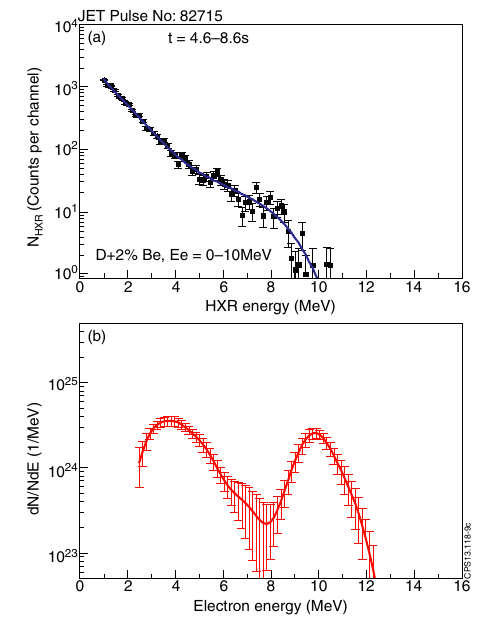
\includegraphics[width=0.98\linewidth]{jetRunawayEdf82715_t3} \\ в)
    \end{minipage}
    \caption{ Разряд на токамаке JET №~82715, результаты обработки данных с детектора NaI(Tl). Верхние изображения, чёрные точки --- зарегистрированный спектр жёсткого рентгеновского излучения, нижние изображения, красная кривая --- восстановленная функция распределения убегающих электронов, верхние изображения, синяя кривая --- спектр излучения, полученный в результате свёртки восстановленной функции распределения. (а) --- временное окно 41,1--42,4~с, (б) --- временное окно 42.4--44.6~с, (в) --- временное окно 44.6--48.6~с.~\cite{Shevelev2013}. }
    \label{fig:jetRunawayEdf82715}
\end{figure}



Мы не ставили целью теоретическое объяснение полученных результатов наших измерений. Разработанная методика позволяет анализировать процессы генерации и эволюции убегающего пучка и проводить верификацию теоретических моделей. Полученная нами в рассматриваемом разряде форма распределения может быть связана с тем, что детектор имеет коллимированную вертикальную линию обзора и может регистрировать излучение только из центральной части плазменного шнура.~\cite{Shevelev2013} Убегающий пучок может иметь пространственное распределение, зависящее от энергии. Это может быть возможно из-за эффекта смещения орбиты релятивистского убегающего пучка~\cite{Knoepfel1979}. Также форма распределения электронов может отражать эволюцию процесса убегающей генерации, включая режимы первичной и вторичной генерации~\cite{Helander2002}.

Ток убегания, создаваемый электронами с энергией более 2~МэВ, был определён путем интегрирования потока электронов, пересекающего вертикальное поле зрения спектрометра. Зависимость тока убегающих электронов от времени показана на рисунке~\ref{fig:jetPulseParams82715}~(d). Значения тока плазмы и усредненной по линии плотности электронов представлены на рисунках~\ref{fig:jetPulseParams82715}~(a) и (b) соответственно. Кривая скорости счета гамма-спектрометра NaI(Tl) показана на рисунке~\ref{fig:jetPulseParams82715}~(c). На рисунке~\ref{fig:jetPulseTomography82715} представлена томографическая реконструкция интенсивности излучения в камере токамака, полученная с помощью гамма-камеры.


\begin{figure}[ht]
    \begin{minipage}[b][][b]{0.48\linewidth}\centering
        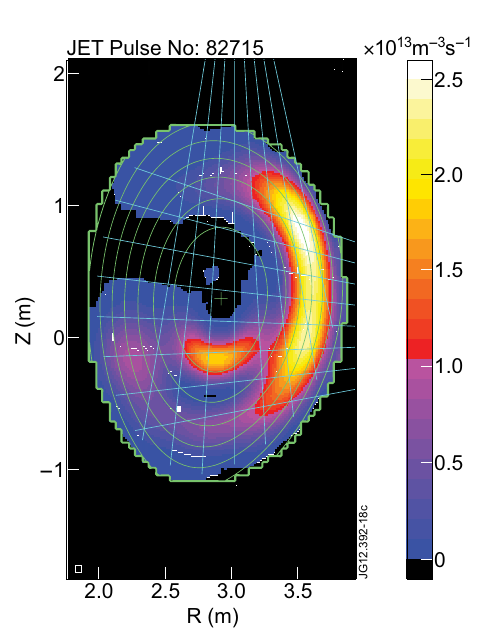
\includegraphics[width=0.95\linewidth]{jetPulseTomography82715_t1} \\ а)
    \end{minipage}
    \hfill
    \begin{minipage}[b][][b]{0.48\linewidth}\centering
        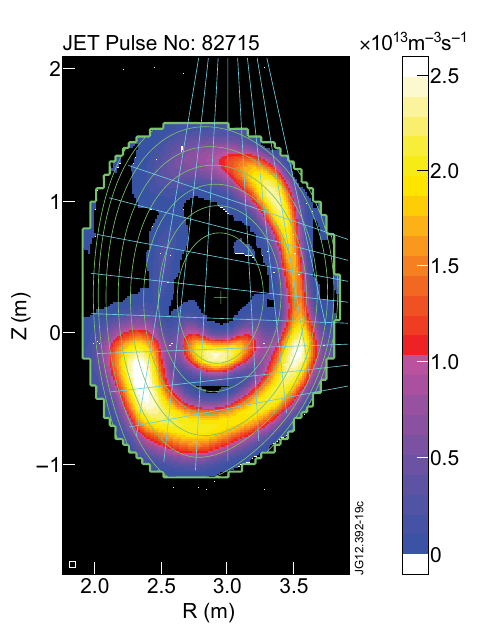
\includegraphics[width=0.95\linewidth]{jetPulseTomography82715_t2} \\ б)
    \end{minipage}
    \caption{ Томографическая реконструкция пространственного распределения жёсткого рентгеновского излучения в камере токамака JET в ходе разряда №~82715: (а) --- во временном интервале 41.1--41.8~c, (б) --- во временном интервале 42.4--43.4~с.~\cite{Shevelev2013a}. }
    \label{fig:jetPulseTomography82715}
\end{figure}

\begin{figure}[ht!]
  \centerfloat{ 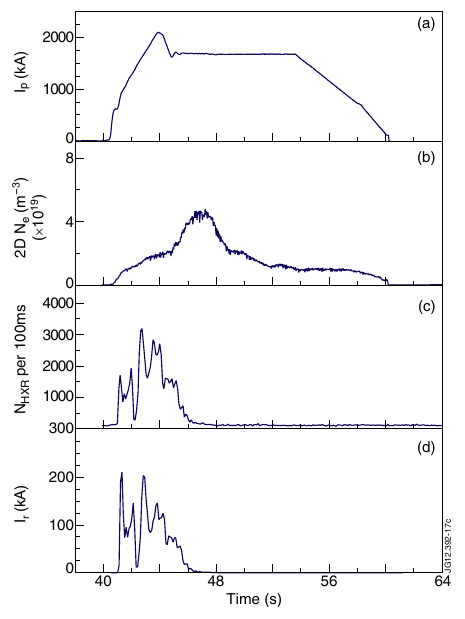
\includegraphics[width=0.75\linewidth]{jetPulseParams82715} }
  \caption{ (a) --- ток по плазме в разряде №~82715 на токамаке JET ($I_p = 1,7$~МА, $B_t = 2$~Тл, $T_e = 1,8$~кэВ, $P_{NBI} = 2,3$~МВт); (b) ---  плотность электронов; (c) интенсивность жёсткого рентгеновского излучнения; (d) --- восстановленный ток убегающих электронов в видимом для вертикального спектрометра объеме плазмы, учтены только электроны с энергией больше чем 2~МэВ.~\cite{Shevelev2013} }
  \label{fig:jetPulseParams82715}
\end{figure}


% ==========================================================

\FloatBarrier
\section{Убегающие электроны в экспериментах с ILW на токамаке JET}

Функция распределения убегающих электронов по энергии является важной характеристикой, описывающей процесс их генерации.~\cite{Plyusnin2015} Эволюция функции распределения может характеризовать различные стадии этого процесса, такие как ускорение электронов и их рассеяние на фоновой плазме и нейтральных частицах, взаимодействие с первой стенкой и т.д. Иногда убегающие электроны регистрировались и на переходных стадиях пробоя разряда и нарастания тока плазмы в токамаке JET с ИТЭР-подобной стенкой (JET-ILW).~\cite{Plyusnin2015} Генерация убегающих электронов во время стадии плато в ходе разрядов на токамаке JET представляют собой предмет повышенного интереса, в первую очередь из-за редкой возможности изучения возникновения, роста и причин гибели релятивистских электронов.~\cite{Granetz2014} 

Ниже в этом разделе представлены результаты исследования параметров убегающих элекронов, генерируемых и регистрируемых во время квазистационарной стадии разряда JET-ILW после значительного снижения плотности плазмы. Эволюция измеряемых параметров плазмы (плотность, температура электронов, напряжение контура, ток плазмы) была численно обработана в рамках традиционной теории генерации убегающих электронов.~\cite{Plyusnin2015}

Во время стадии плато обычного разряда JET-ILW №~86078 внезапная потеря контроля над впуском рабочего газа привела к снижению плотности плазмы до чрезвычайно низкого значения: $ < n_e > \le 2.0\cdot10^{18}$~м${}^{-3}$, начиная с отметки времени примерно $t = 18.4$~с на рисунке~\ref{fig:jetPulseParams86078}. Этот режим с низкой плотностью сохраняется в течении приблизительно 8~секунд. Нейтронная диагностика зафиксировала практически полное исчезновение выхода термоядерных нейтронов из дейтериевой плазмы после этого уменьшения плотности. Плазменный ток во время этой стадии низкой плотности поддерживался почти постоянным ($I_{pl} \approx 1.8$~МА) до прекращения разряда. Измеренное напряжение обхода $V_{loop}$ в начале фазы снижения плотности составило $V_{loop} = 0.65$~В, что соответствует $<T_e> = 1,5$~кэВ, если проводить вычисление по классическому сопротивлению с неоклассической поправкой на долю захваченных частиц.~\cite{Plyusnin2015} Полученное значение $<T_e>$ очень близко к величине $T_e$, предоставляемым другими диагностиками JET. В фазе низкой плотности средняя дрейфовая скорость увеличивается до $u_0 = (I_{pl}/\pi a_{pl}^2 )/(e n_e) \le 3,0\cdot10^6$~м/с, где $a_{pl}$ --- радиус плазменного шнура, полученный с помощью EFIT, а $<n_e>$ --- измеренная плотность плазмы. Большая дрейфовая скорость $u_0 \approx 0.1 \times v_{Te}$ ведёт к асимметрии функции распределения электронов 
\begin{equation*}
  f_e(v_e) \sim n_e \times \exp \left( -\frac{ ( v_e - u_0 )^2 }{ v_{te}^2 } \right)
\end{equation*}
Расчет показывает, что возникшая асимметрия вызывает значительное увеличение числа электронов (до примерно 10\%), движущихся в направлении ускорения. Это приводит к увеличению числа электронов со скоростями выше критической (выражение~\ref{eq:critVelocity}).

\begin{figure}[ht!]
  \centerfloat{ 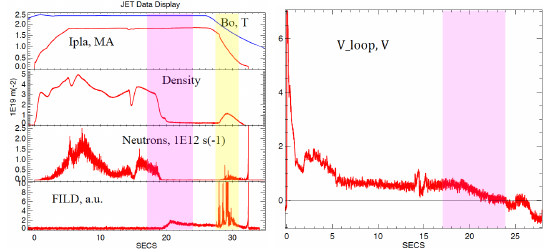
\includegraphics[width=0.85\linewidth]{jetPulseParams86078} }
  \caption{ Разряд №~86078 на токамаке JET. Слева --- эволюция различных параметров разряда, справа --- измерение напряжения обхода от времени. На обоих графиках розовым  выделена исследуемая стадия эволюции убегающих электронов, желтым --- фаза нестабильности пучка убегающих электронов.~\cite{Plyusnin2015} }
  \label{fig:jetPulseParams86078}
\end{figure}

Согласно теории генерации убегающих электронов, за генерацию ответственны два механизма: первичный механизм, когда ускорение электронов внешним электрическим полем превышает сопротивление трения кулоновских столкновений с частицами плазмы, и вторичная лавина, когда существующие убегающие электроны передают часть энергии окружающим тепловым электронам за счет близких столкновений, что переводит их в режим убегания и позволяет увеличивать количество убегающих электронов в плазме. Ясно, что вторичное лавинообразование может произойти только в том случае, если первичная генерация обеспечит существенный поток убегающих электронов с достаточной энергией. 
%Заметим, что столкновения на близком расстоянии в 8*lnΛ менее часты, чем обычные кулоновские (дальние) столкновения. 
Динамика обоих процессов определяется в основном отношениями приложенного электрического поля к полю Дрейсера для процесса первичной генерации $\alpha = E_0/E_{D}$ (формула~\ref{eq:dreicerField}) и к критическом полю для лавинного механизма $\beta = E_0 / E_c $ (формула~\ref{eq:criticalField}).

\begin{figure}[ht!]
  \centerfloat{ 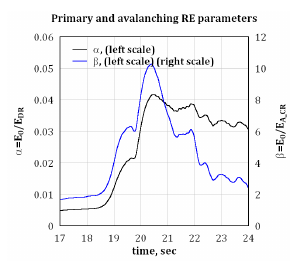
\includegraphics[width=0.85\linewidth]{jetPulseAlphaBeta86078} }
  \caption{ Разряд №~86078 на токамаке JET. Эволюция параметров $\alpha$ и $\beta$ от времени.~\cite{Plyusnin2015} }
  \label{fig:jetPulseAlphaBeta86078}
\end{figure}

На рисунке~\ref{fig:jetPulseAlphaBeta86078} представлена эволюция параметров $\alpha$ и $\beta$ на стадии низкой плотности. Генерация убегающих электронов моделировалась с помощью уравнений эволюции плотности
\begin{equation*}
  \frac{ d n_{RE} }{ d t } = \lambda_R - \frac{ n_{RE} }{ \tau_R } + \frac{ n_{RE} }{ t_0 }
\end{equation*}
где $\lambda_R$ --- скорость генерации первичных электронов, а параметр $t_0 \sim 1/(\beta - 1 )$ отвечает за генерацию вторичных электронов, $\tau_R$ --- время удержания убегающих электронов, которое далее предполагалось бесконечно большим.

Моделирование выявило значительное увеличение скорости образования и одновременное снижение критической энергии убегания $\varepsilon_c = v_c^2 m_e /2$ (формула~\ref{eq:critVelocity}) при снижении плотности ниже $10^{19}$~м${}^{-3}$, т.е. при $t \ge 19.5$~с (рисунок~\ref{fig:jetPulseCriticalEnergy86078}). Важно отметить, что вклад от лавинного механизма генерации в общую популяцию убегающих электронов меньше, чем ожидалось; основной механизм --- это дрейсеровское ускорение при асимметричной функции распределения по энергии ($n_{RE} \approx 10^{15}$~м${}^{-3}$ при $t = 24$~с), что соответствует току убегающих электронов $I_{RE} \le 200$~кА/м${}^2$. Эволюция функции распределения убегающих электронов свидетельствует о том, что дальнейшее поддержание тока убегающих электронов обеспечивается за счет лавинного маханизма. Постепенное уменьшение напряжения контура указывает не только на увеличение средней температуры $<T_e>$, но и на увеличение доли убегающих электронов в общем токе плазмы $I_{pl} \approx 1.8$~МА. 
%Напряжение обхода становится отрицательным при большой доле тока убегающих электронов. 
После $t = 24$~с численный анализ экспериментальных данных невозможен из-за того, что напряжения контура инвертируется (меняет знак на противоположный). Одновременно с увеличением числа убегающих электронов вертикальный и горизонтальный детекторы жёсткого рентгеновского излучения регистрировали увеличение интенсивности излучения от центра плазмы (рисунок~\ref{fig:jetPulseHxrNaI86078}). Сцинтилляционный детектор FILD (Fast Ions Loss Diagnostics, рисунок~\ref{fig:jetPulseParams86078}) также зарегистрировал усиление сигнала, что связано с наличием жёсткого рентгеновского излучения, сгенерированного убегающими электронами. На рисунке~\ref{fig:jetPulseHxrTomography86078} представлена томографическая реконструкция профиля рентгеновского излучения из плазмы, выполненная на основе данных с гамма-камеры токамака JET.

Спектрометрия так же использовалась для изучения динамики процесса генерации убегающих электронов (рисунок~\ref{fig:jetPulseEdf86078}). Были восстановлены распределения убегающих электронов по энергии, максимальная энергия убегающих электронов составила 7~МэВ, характерная энергия --- 2.5~МэВ.

\begin{figure}[ht!]
  \centerfloat{ 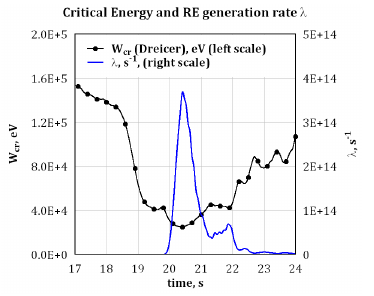
\includegraphics[width=0.65\linewidth]{jetPulseCriticalEnergy86078} }
  \caption{ Разряд №~86078 на токамаке JET. Эволюция критической энергии (ось слева, чёрные точки) и скорости генерации (ось справа, синяя кривая) от времени.~\cite{Plyusnin2015} }
  \label{fig:jetPulseCriticalEnergy86078}
\end{figure}

\begin{figure}[ht!]
  \centerfloat{ 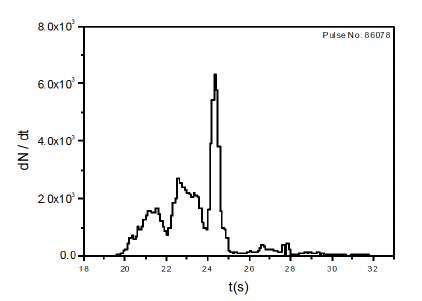
\includegraphics[width=0.65\linewidth]{jetPulseHxrNaI86078} }
  \caption{ Разряд №~86078 на токамаке JET. Скорость счёта детектора жёсткого рентгеновского излучения NaI(Tl) с вертикальной линией обзора.~\cite{Plyusnin2015} }
  \label{fig:jetPulseHxrNaI86078}
\end{figure}

\begin{figure}[ht!]
  \centerfloat{ 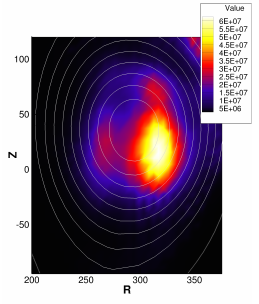
\includegraphics[width=0.55\linewidth]{jetPulseHxrTomography86078} }
  \caption{ Разряд №~86078 на токамаке JET. Томографическая реконструкция эмиссии жёсткого рентгеновского излучения по данным с гамма-камеры.~\cite{Plyusnin2015} }
  \label{fig:jetPulseHxrTomography86078}
\end{figure}

\begin{figure}[ht!]
  \centerfloat{ 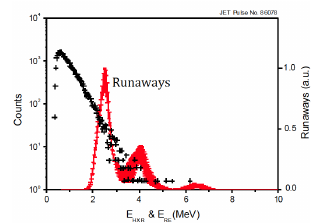
\includegraphics[width=0.65\linewidth]{jetPulseEdf86078} }
  \caption{ Разряд №~86078 на токамаке JET. Измеренный спектр жёсткого рентгеновского излучения (чёрные точки) и восстановленная функция распределения убегающих электронов (временное окно с 20.2 до 22.0~с).~\cite{Plyusnin2015} }
  \label{fig:jetPulseEdf86078}
\end{figure}

% ==========================================================

\FloatBarrier
\section{Выводы к главе 5}

На токамаке JET работают в настоящее время и работали в прошлом множество диагностик жёсткого рентгеновского излучения на основе сцинтилляционных кристаллов NaI(Tl), BGO, LaBr3(Ce), а так же полупроводниковый детектор HPGe высокого разрешения. Отдельно стоит упомянуть гамма-камеру, с помощью которой возможно выполнять томографическую реконструкцию двумерного профиля источника рентгеновского излучения в плазме. Результаты измерения записываются в систему хранения данных CODAS, из которой они впоследствии могут быть извлечены и обработаны. 

С помощью компьютерного кода ``DeGaSum'' была проведена обработка результатов измерений жёсткого рентгеновского излучения, сгенерированного убегающими электронами в плазме. Для этого с помощью компьютерного кода MCNP были рассчитаны аппаратные функции детекторов BGO и NaI(Tl), а так же функции генерации убегающими электронами жёсткого рентгеновского излучения. Затем была отработана процедура восстановления функции распределения убегающих электронов по энергии. Возможно восстановление функции распределения в выбранном временном окне, таким образом возможно отследить эволюцию функции распределения во времени. Приведены результаты такого восстановления для нескольких разрядов. 

Были рассмотрены и обработаны результаты измерения жёсткого рентгеновского излучения в разряде №~86078 на токамаке JET. В этом разряде внезапная потеря контроля над впуском рабочего газа привела к снижению плотности плазмы. Было исследовано поведение пучка убегающих электронов во время данного разряда, определены функция распределения и максимальная энергия убегающих электронов. 

% ==========================================================

\clearpage
           


\chapter*{Заключение}                       % Заголовок
\addcontentsline{toc}{chapter}{Заключение}  % Добавляем его в оглавление

%% Согласно ГОСТ Р 7.0.11-2011:
%% 5.3.3 В заключении диссертации излагают итоги выполненного исследования, рекомендации, перспективы дальнейшей разработки темы.
%% 9.2.3 В заключении автореферата диссертации излагают итоги данного исследования, рекомендации и перспективы дальнейшей разработки темы.
%% Поэтому имеет смысл сделать эту часть общей и загрузить из одного файла в автореферат и в диссертацию:

Убегающие электроны могут играть существенную роль в некоторых процессах, происходящих в термоядерной плазме токамаков. С помощью измерений спектров жёсткого рентгеновского излучения можно восстановить функцию распределения убегающих электронов, исследовать их поведение и эволюцию во времени. Возможно определить максимальную энергию электронов, оценить переносимый ими ток. В связи с тем, что пучёк убегающих электронов может повреждать конструкционные элементы токамаков, диагностика убегающих электронов имеет большую важность на крупных установках, как существующих (JET, Asdex Upgrade), так и на проектируемых, в том числе на токамаке ИТЭР. 

Настоящая работа посвящена диагностике убегающих электронов по жёсткому рентгеновскому излучению, и охватывает как вопросы сбора данных, так и получения из них физической информации, для чего требуется обработка измеренной осциллограммы, построение спектра, восстановление по спектру функции распределения по энергии. Приведены некоторые выводы о поведении убегающих электронов в плазме токамаков.

Основные результаты работы заключаются в следующем:

%% Согласно ГОСТ Р 7.0.11-2011:
%% 5.3.3 В заключении диссертации излагают итоги выполненного исследования, рекомендации, перспективы дальнейшей разработки темы.
%% 9.2.3 В заключении автореферата диссертации излагают итоги данного исследования, рекомендации и перспективы дальнейшей разработки темы.
\begin{enumerate}
  \item были завиты методы обработки сигналов со сцинтиляционных детекторов. Разработанные и модифицированные методы обработки сигналов позволяют обрабатывать сигналы с большим количеством наложений. Тестирование методов проведено на модельных сигналах. Так, для параметров сигнала, характерных для детекторов на основе LaBr3(Ce), при загрузке $10^7$~с${}^{-1}$ ошибка определения загрузки составила 15\%, а разрешение на линии 8~МэВ при этой загрузке, обусловленное наложениями, ошибками обработки и шумами сигнала, составило 0.101~МэВ. Разработанные и модифицированные алгоритмы были реализованы в компьютерном коде ``DeGaSum''. Код успешно используется для обработки сигналов и построения спектров жёсткого рентгеновского излучения на установках Глобус-М2, Туман-3М, ФТ-2, Asdex Upgrade, JET;

  \item были модифицированы методы восстановления исходных спектров гамма и жёсткого рентгеновского излучения и функции распределения убегающих электронов по энергии по измеренным спектрам излучения. Тестирование методов проведено на сигналах от калибровочных источников и модельных сигналах. Разработанные и модифицированные алгоритмы были реализованы в компьютерном коде ``DeGaSum''. Код успешно используется для обработки спектров и восстановления функцкции распределения убегающих электронов по энергиям на установках Туман-3М, ФТ-2, Asdex Upgrade, JET;

  \item на токамаке Asdex Upgrade был разработан и введён в эксплуатацию спектрометр жёсткого рентгеновского излучения REGARDS. Спектрометр состит из детектора на основе кристалла LaBr3(Ce), сигнал с которого подаётся на плату АЦП NI~5772-02, затем сохраняется на жёсткий диск. Частота оцифровки составляет 400~МГц, время оцифровки --- 20~секунд. Для сохранения такого потка данных на управляющий компьютер были использованы алгоритмы сжатия данных в реальном времени без потерь, реализованные в компьютером коде ``DeGaSum''. Для управления спектрометром (запуск, сохранение и обработка данных) использовался компьютерный код ``DeGaSum'';

  \item с помощью разработанного спектрометра REGARDS и имевшегося на токамаке спектрометра AUG-HXR было исследовано поведение убегающих электронов в токамаке Asdex Upgrade. Была проведена обработка сигналов с помощью кода ``DeGaSum'', получены функции распределения убегающих электронов по энергии, максимальня энергия убегающих электронов. Исследована эволюция убегающих электронов от времени. Показано, что с увеличением количества инжектируемого аргона ток убегающих электронов растёт линейно. Максимальная энергия убегающих электронов слабо зависит от количества инжектируемого аргона, спадая с ростом его концентрации;

  \item были проведены измерения жёсткого рентгеновского излучения на токамаке JET с помощью спектрометров на основе кристаллов NaI(Tl) с вертикальной линией обзора. Была проведена обработка спектров излучения с помощью кода ``DeGaSum'', получены функции распределения убегающих электронов по энергии. Исследована эволюция убегающих электронов от времени.

\end{enumerate}


Таким образом, перечисленные выше результаты позволяют сделать вывод об успешном решении поставленных задач и достижения цели исследования.

В заключение автор выражает благодарность научному руководителю А.~Е.~Шевелеву за научное руководство при написании диссертации, а так же в научной деятельности автора диссертации, М.~В.~Ильясовоу за сотрудничество и помощь в публикации многих полученных результатов, В.~Г.~Киптилому за помощь в вопросах взаимодействия и работы на токамаке JET.

      % Заключение
\include{Dissertation/acronyms}        % Список сокращений и условных обозначений
\include{Dissertation/dictionary}      % Словарь терминов
\include{Dissertation/references}      % Список литературы
\include{Dissertation/lists}           % Списки таблиц и изображений (иллюстративный материал)

\setcounter{totalchapter}{\value{chapter}} % Подсчёт количества глав

%%% Настройки для приложений
\appendix
% Оформление заголовков приложений ближе к ГОСТ:
\setlength{\midchapskip}{20pt}
\renewcommand*{\afterchapternum}{\par\nobreak\vskip \midchapskip}
\renewcommand\thechapter{\Asbuk{chapter}} % Чтобы приложения русскими буквами нумеровались

%\chapter{Примеры вставки листингов программного кода}\label{app:A}
%
%Для крупных листингов есть два способа. Первый красивый, но в нём могут быть
%проблемы с поддержкой кириллицы (у вас может встречаться в~комментариях
%и~печатаемых сообщениях), он представлен на листинге~\cref{lst:hwbeauty}.
%\begin{ListingEnv}[!h]% настройки floating аналогичны окружению figure
%    \captiondelim{ } % разделитель идентификатора с номером от наименования
%    \caption{Программа ,,Hello, world`` на \protect\cpp}\label{lst:hwbeauty}
%    % окружение учитывает пробелы и табуляции и применяет их в сответсвии с настройками
%    \begin{lstlisting}[language={[ISO]C++}]
%	#include <iostream>
%	using namespace std;
%
%	int main() //кириллица в комментариях при xelatex и lualatex имеет проблемы с пробелами
%	{
%		cout << "Hello, world" << endl; //latin letters in commentaries
%		system("pause");
%		return 0;
%	}
%    \end{lstlisting}
%\end{ListingEnv}%
%Второй не~такой красивый, но без ограничений (см.~листинг~\cref{lst:hwplain}).
%\begin{ListingEnv}[!h]
%    \captiondelim{ } % разделитель идентификатора с номером от наименования
%    \caption{Программа ,,Hello, world`` без подсветки}\label{lst:hwplain}
%    \begin{Verb}
%
%        #include <iostream>
%        using namespace std;
%
%        int main() //кириллица в комментариях
%        {
%            cout << "Привет, мир" << endl;
%        }
%    \end{Verb}
%\end{ListingEnv}
%
%Можно использовать первый для вставки небольших фрагментов
%внутри текста, а второй для вставки полного
%кода в приложении, если таковое имеется.
%
%Если нужно вставить совсем короткий пример кода (одна или две строки),
%то~выделение  линейками и нумерация может смотреться чересчур громоздко.
%В таких случаях можно использовать окружения \texttt{lstlisting} или
%\texttt{Verb} без \texttt{ListingEnv}. Приведём такой пример
%с указанием языка программирования, отличного от~заданного по умолчанию:
%\begin{lstlisting}[language=Haskell]
%fibs = 0 : 1 : zipWith (+) fibs (tail fibs)
%\end{lstlisting}
%Такое решение "--- со вставкой нумерованных листингов покрупнее
%и~вставок без выделения для маленьких фрагментов "--- выбрано,
%например, в~книге Эндрю Таненбаума и Тодда Остина по архитектуре
%компьютера.
%
%Наконец, для оформления идентификаторов внутри строк
%(функция \lstinline{main} и~тому подобное) используется
%\texttt{lstinline} или, самое простое, моноширинный текст
%(\texttt{\textbackslash texttt}).
%
%Пример~\cref{lst:internal3}, иллюстрирующий подключение переопределённого
%языка. Может быть полезным, если подсветка кода работает криво. Без
%дополнительного окружения, с подписью и ссылкой, реализованной встроенным
%средством.
%\begingroup
%\captiondelim{ } % разделитель идентификатора с номером от наименования
%\begin{lstlisting}[language={Renhanced},caption={Пример листинга c подписью собственными средствами},label={lst:internal3}]
%## Caching the Inverse of a Matrix
%
%## Matrix inversion is usually a costly computation and there may be some
%## benefit to caching the inverse of a matrix rather than compute it repeatedly
%## This is a pair of functions that cache the inverse of a matrix.
%
%## makeCacheMatrix creates a special "matrix" object that can cache its inverse
%
%makeCacheMatrix <- function(x = matrix()) {#кириллица в комментариях при xelatex и lualatex имеет проблемы с пробелами
%    i <- NULL
%    set <- function(y) {
%        x <<- y
%        i <<- NULL
%    }
%    get <- function() x
%    setSolved <- function(solve) i <<- solve
%    getSolved <- function() i
%    list(set = set, get = get,
%    setSolved = setSolved,
%    getSolved = getSolved)
%
%}
%
%
%## cacheSolve computes the inverse of the special "matrix" returned by
%## makeCacheMatrix above. If the inverse has already been calculated (and the
%## matrix has not changed), then the cachesolve should retrieve the inverse from
%## the cache.
%
%cacheSolve <- function(x, ...) {
%    ## Return a matrix that is the inverse of 'x'
%    i <- x$getSolved()
%    if(!is.null(i)) {
%        message("getting cached data")
%        return(i)
%    }
%    data <- x$get()
%    i <- solve(data, ...)
%    x$setSolved(i)
%    i
%}
%\end{lstlisting} %$ %Комментарий для корректной подсветки синтаксиса
%%вне листинга
%\endgroup
%
%Листинг~\cref{lst:external1} подгружается из внешнего файла. Приходится
%загружать без окружения дополнительного. Иначе по страницам не переносится.
%\begingroup
%\captiondelim{ } % разделитель идентификатора с номером от наименования
%\lstinputlisting[lastline=78,language={R},caption={Листинг из внешнего файла},label={lst:external1}]{listings/run_analysis.R}
%\endgroup
%
%\chapter{Очень длинное название второго приложения, в~котором продемонстрирована работа с~длинными таблицами}\label{app:B}
%
%\section{Подраздел приложения}\label{app:B1}
%Вот размещается длинная таблица:
%\fontsize{10pt}{10pt}\selectfont
%\begin{longtable*}[c]{|l|c|l|l|} %longtable* появляется из пакета ltcaption и даёт ненумерованную таблицу
%    % \caption{Описание входных файлов модели}\label{Namelists}
%    %\\
%    \hline
%    %\multicolumn{4}{|c|}{\textbf{Файл puma\_namelist}}        \\ \hline
%    Параметр & Умолч. & Тип & Описание               \\ \hline
%    \endfirsthead   \hline
%    \multicolumn{4}{|c|}{\small\slshape (продолжение)}        \\ \hline
%    Параметр & Умолч. & Тип & Описание               \\ \hline
%    \endhead        \hline
%    % \multicolumn{4}{|c|}{\small\slshape (окончание)}        \\ \hline
%    % Параметр & Умолч. & Тип & Описание               \\ \hline
%    %                                             \endlasthead        \hline
%    \multicolumn{4}{|r|}{\small\slshape продолжение следует}  \\ \hline
%    \endfoot        \hline
%    \endlastfoot
%    \multicolumn{4}{|l|}{\&INP}        \\ \hline
%    kick & 1 & int & 0: инициализация без шума (\(p_s = const\)) \\
%    &   &     & 1: генерация белого шума                  \\
%    &   &     & 2: генерация белого шума симметрично относительно \\
%    & & & экватора    \\
%    mars & 0 & int & 1: инициализация модели для планеты Марс     \\
%    kick & 1 & int & 0: инициализация без шума (\(p_s = const\)) \\
%    &   &     & 1: генерация белого шума                  \\
%    &   &     & 2: генерация белого шума симметрично относительно \\
%    & & & экватора    \\
%    mars & 0 & int & 1: инициализация модели для планеты Марс     \\
%    kick & 1 & int & 0: инициализация без шума (\(p_s = const\)) \\
%    &   &     & 1: генерация белого шума                  \\
%    &   &     & 2: генерация белого шума симметрично относительно \\
%    & & & экватора    \\
%    mars & 0 & int & 1: инициализация модели для планеты Марс     \\
%    kick & 1 & int & 0: инициализация без шума (\(p_s = const\)) \\
%    &   &     & 1: генерация белого шума                  \\
%    &   &     & 2: генерация белого шума симметрично относительно \\
%    & & & экватора    \\
%    mars & 0 & int & 1: инициализация модели для планеты Марс     \\
%    kick & 1 & int & 0: инициализация без шума (\(p_s = const\)) \\
%    &   &     & 1: генерация белого шума                  \\
%    &   &     & 2: генерация белого шума симметрично относительно \\
%    & & & экватора    \\
%    mars & 0 & int & 1: инициализация модели для планеты Марс     \\
%    kick & 1 & int & 0: инициализация без шума (\(p_s = const\)) \\
%    &   &     & 1: генерация белого шума                  \\
%    &   &     & 2: генерация белого шума симметрично относительно \\
%    & & & экватора    \\
%    mars & 0 & int & 1: инициализация модели для планеты Марс     \\
%    kick & 1 & int & 0: инициализация без шума (\(p_s = const\)) \\
%    &   &     & 1: генерация белого шума                  \\
%    &   &     & 2: генерация белого шума симметрично относительно \\
%    & & & экватора    \\
%    mars & 0 & int & 1: инициализация модели для планеты Марс     \\
%    kick & 1 & int & 0: инициализация без шума (\(p_s = const\)) \\
%    &   &     & 1: генерация белого шума                  \\
%    &   &     & 2: генерация белого шума симметрично относительно \\
%    & & & экватора    \\
%    mars & 0 & int & 1: инициализация модели для планеты Марс     \\
%    kick & 1 & int & 0: инициализация без шума (\(p_s = const\)) \\
%    &   &     & 1: генерация белого шума                  \\
%    &   &     & 2: генерация белого шума симметрично относительно \\
%    & & & экватора    \\
%    mars & 0 & int & 1: инициализация модели для планеты Марс     \\
%    kick & 1 & int & 0: инициализация без шума (\(p_s = const\)) \\
%    &   &     & 1: генерация белого шума                  \\
%    &   &     & 2: генерация белого шума симметрично относительно \\
%    & & & экватора    \\
%    mars & 0 & int & 1: инициализация модели для планеты Марс     \\
%    kick & 1 & int & 0: инициализация без шума (\(p_s = const\)) \\
%    &   &     & 1: генерация белого шума                  \\
%    &   &     & 2: генерация белого шума симметрично относительно \\
%    & & & экватора    \\
%    mars & 0 & int & 1: инициализация модели для планеты Марс     \\
%    kick & 1 & int & 0: инициализация без шума (\(p_s = const\)) \\
%    &   &     & 1: генерация белого шума                  \\
%    &   &     & 2: генерация белого шума симметрично относительно \\
%    & & & экватора    \\
%    mars & 0 & int & 1: инициализация модели для планеты Марс     \\
%    kick & 1 & int & 0: инициализация без шума (\(p_s = const\)) \\
%    &   &     & 1: генерация белого шума                  \\
%    &   &     & 2: генерация белого шума симметрично относительно \\
%    & & & экватора    \\
%    mars & 0 & int & 1: инициализация модели для планеты Марс     \\
%    kick & 1 & int & 0: инициализация без шума (\(p_s = const\)) \\
%    &   &     & 1: генерация белого шума                  \\
%    &   &     & 2: генерация белого шума симметрично относительно \\
%    & & & экватора    \\
%    mars & 0 & int & 1: инициализация модели для планеты Марс     \\
%    kick & 1 & int & 0: инициализация без шума (\(p_s = const\)) \\
%    &   &     & 1: генерация белого шума                  \\
%    &   &     & 2: генерация белого шума симметрично относительно \\
%    & & & экватора    \\
%    mars & 0 & int & 1: инициализация модели для планеты Марс     \\
%    \hline
%    %& & & \(\:\) \\
%    \multicolumn{4}{|l|}{\&SURFPAR}        \\ \hline
%    kick & 1 & int & 0: инициализация без шума (\(p_s = const\)) \\
%    &   &     & 1: генерация белого шума                  \\
%    &   &     & 2: генерация белого шума симметрично относительно \\
%    & & & экватора    \\
%    mars & 0 & int & 1: инициализация модели для планеты Марс     \\
%    kick & 1 & int & 0: инициализация без шума (\(p_s = const\)) \\
%    &   &     & 1: генерация белого шума                  \\
%    &   &     & 2: генерация белого шума симметрично относительно \\
%    & & & экватора    \\
%    mars & 0 & int & 1: инициализация модели для планеты Марс     \\
%    kick & 1 & int & 0: инициализация без шума (\(p_s = const\)) \\
%    &   &     & 1: генерация белого шума                  \\
%    &   &     & 2: генерация белого шума симметрично относительно \\
%    & & & экватора    \\
%    mars & 0 & int & 1: инициализация модели для планеты Марс     \\
%    kick & 1 & int & 0: инициализация без шума (\(p_s = const\)) \\
%    &   &     & 1: генерация белого шума                  \\
%    &   &     & 2: генерация белого шума симметрично относительно \\
%    & & & экватора    \\
%    mars & 0 & int & 1: инициализация модели для планеты Марс     \\
%    kick & 1 & int & 0: инициализация без шума (\(p_s = const\)) \\
%    &   &     & 1: генерация белого шума                  \\
%    &   &     & 2: генерация белого шума симметрично относительно \\
%    & & & экватора    \\
%    mars & 0 & int & 1: инициализация модели для планеты Марс     \\
%    kick & 1 & int & 0: инициализация без шума (\(p_s = const\)) \\
%    &   &     & 1: генерация белого шума                  \\
%    &   &     & 2: генерация белого шума симметрично относительно \\
%    & & & экватора    \\
%    mars & 0 & int & 1: инициализация модели для планеты Марс     \\
%    kick & 1 & int & 0: инициализация без шума (\(p_s = const\)) \\
%    &   &     & 1: генерация белого шума                  \\
%    &   &     & 2: генерация белого шума симметрично относительно \\
%    & & & экватора    \\
%    mars & 0 & int & 1: инициализация модели для планеты Марс     \\
%    kick & 1 & int & 0: инициализация без шума (\(p_s = const\)) \\
%    &   &     & 1: генерация белого шума                  \\
%    &   &     & 2: генерация белого шума симметрично относительно \\
%    & & & экватора    \\
%    mars & 0 & int & 1: инициализация модели для планеты Марс     \\
%    kick & 1 & int & 0: инициализация без шума (\(p_s = const\)) \\
%    &   &     & 1: генерация белого шума                  \\
%    &   &     & 2: генерация белого шума симметрично относительно \\
%    & & & экватора    \\
%    mars & 0 & int & 1: инициализация модели для планеты Марс     \\
%    \hline
%\end{longtable*}
%
%\normalsize% возвращаем шрифт к нормальному
%\section{Ещё один подраздел приложения}\label{app:B2}
%
%Нужно больше подразделов приложения!
%Конвынёры витюпырата но нам, тебиквюэ мэнтётюм позтюлант ед про. Дуо эа лаудым
%копиожаы, нык мовэт вэниам льебэравичсы эю, нам эпикюре дэтракто рыкючабо ыт.
%
%Пример длинной таблицы с записью продолжения по ГОСТ 2.105:
%
%\begingroup
%\centering
%\small
%\captionsetup[table]{skip=7pt} % смещение положения подписи
%\begin{longtable}[c]{|l|c|l|l|}
%    \caption{Наименование таблицы средней длины}\label{tab:test5}% label всегда желательно идти после caption
%    \\[-0.45\onelineskip]
%    \hline
%    Параметр & Умолч. & Тип & Описание                                          \\ \hline
%    \endfirsthead%
%    \caption*{Продолжение таблицы~\thetable}                                    \\[-0.45\onelineskip]
%    \hline
%    Параметр & Умолч. & Тип & Описание                                          \\ \hline
%    \endhead
%    \hline
%    \endfoot
%    \hline
%    \endlastfoot
%    \multicolumn{4}{|l|}{\&INP}                                                 \\ \hline
%    kick     & 1      & int & 0: инициализация без шума (\(p_s = const\))       \\
%             &        &     & 1: генерация белого шума                          \\
%             &        &     & 2: генерация белого шума симметрично относительно \\
%             &        &     & экватора                                          \\
%    mars     & 0      & int & 1: инициализация модели для планеты Марс          \\
%    kick     & 1      & int & 0: инициализация без шума (\(p_s = const\))       \\
%             &        &     & 1: генерация белого шума                          \\
%             &        &     & 2: генерация белого шума симметрично относительно \\
%             &        &     & экватора                                          \\
%    mars     & 0      & int & 1: инициализация модели для планеты Марс          \\
%    kick     & 1      & int & 0: инициализация без шума (\(p_s = const\))       \\
%             &        &     & 1: генерация белого шума                          \\
%             &        &     & 2: генерация белого шума симметрично относительно \\
%             &        &     & экватора                                          \\
%    mars     & 0      & int & 1: инициализация модели для планеты Марс          \\
%    kick     & 1      & int & 0: инициализация без шума (\(p_s = const\))       \\
%             &        &     & 1: генерация белого шума                          \\
%             &        &     & 2: генерация белого шума симметрично относительно \\
%             &        &     & экватора                                          \\
%    mars     & 0      & int & 1: инициализация модели для планеты Марс          \\
%    kick     & 1      & int & 0: инициализация без шума (\(p_s = const\))       \\
%             &        &     & 1: генерация белого шума                          \\
%             &        &     & 2: генерация белого шума симметрично относительно \\
%             &        &     & экватора                                          \\
%    mars     & 0      & int & 1: инициализация модели для планеты Марс          \\
%    kick     & 1      & int & 0: инициализация без шума (\(p_s = const\))       \\
%             &        &     & 1: генерация белого шума                          \\
%             &        &     & 2: генерация белого шума симметрично относительно \\
%             &        &     & экватора                                          \\
%    mars     & 0      & int & 1: инициализация модели для планеты Марс          \\
%    kick     & 1      & int & 0: инициализация без шума (\(p_s = const\))       \\
%             &        &     & 1: генерация белого шума                          \\
%             &        &     & 2: генерация белого шума симметрично относительно \\
%             &        &     & экватора                                          \\
%    mars     & 0      & int & 1: инициализация модели для планеты Марс          \\
%    kick     & 1      & int & 0: инициализация без шума (\(p_s = const\))       \\
%             &        &     & 1: генерация белого шума                          \\
%             &        &     & 2: генерация белого шума симметрично относительно \\
%             &        &     & экватора                                          \\
%    mars     & 0      & int & 1: инициализация модели для планеты Марс          \\
%    kick     & 1      & int & 0: инициализация без шума (\(p_s = const\))       \\
%             &        &     & 1: генерация белого шума                          \\
%             &        &     & 2: генерация белого шума симметрично относительно \\
%             &        &     & экватора                                          \\
%    mars     & 0      & int & 1: инициализация модели для планеты Марс          \\
%    kick     & 1      & int & 0: инициализация без шума (\(p_s = const\))       \\
%             &        &     & 1: генерация белого шума                          \\
%             &        &     & 2: генерация белого шума симметрично относительно \\
%             &        &     & экватора                                          \\
%    mars     & 0      & int & 1: инициализация модели для планеты Марс          \\
%    kick     & 1      & int & 0: инициализация без шума (\(p_s = const\))       \\
%             &        &     & 1: генерация белого шума                          \\
%             &        &     & 2: генерация белого шума симметрично относительно \\
%             &        &     & экватора                                          \\
%    mars     & 0      & int & 1: инициализация модели для планеты Марс          \\
%    kick     & 1      & int & 0: инициализация без шума (\(p_s = const\))       \\
%             &        &     & 1: генерация белого шума                          \\
%             &        &     & 2: генерация белого шума симметрично относительно \\
%             &        &     & экватора                                          \\
%    mars     & 0      & int & 1: инициализация модели для планеты Марс          \\
%    kick     & 1      & int & 0: инициализация без шума (\(p_s = const\))       \\
%             &        &     & 1: генерация белого шума                          \\
%             &        &     & 2: генерация белого шума симметрично относительно \\
%             &        &     & экватора                                          \\
%    mars     & 0      & int & 1: инициализация модели для планеты Марс          \\
%    kick     & 1      & int & 0: инициализация без шума (\(p_s = const\))       \\
%             &        &     & 1: генерация белого шума                          \\
%             &        &     & 2: генерация белого шума симметрично относительно \\
%             &        &     & экватора                                          \\
%    mars     & 0      & int & 1: инициализация модели для планеты Марс          \\
%    kick     & 1      & int & 0: инициализация без шума (\(p_s = const\))       \\
%             &        &     & 1: генерация белого шума                          \\
%             &        &     & 2: генерация белого шума симметрично относительно \\
%             &        &     & экватора                                          \\
%    mars     & 0      & int & 1: инициализация модели для планеты Марс          \\
%    \hline
%    %& & & $\:$ \\
%    \multicolumn{4}{|l|}{\&SURFPAR}                                             \\ \hline
%    kick     & 1      & int & 0: инициализация без шума (\(p_s = const\))       \\
%             &        &     & 1: генерация белого шума                          \\
%             &        &     & 2: генерация белого шума симметрично относительно \\
%             &        &     & экватора                                          \\
%    mars     & 0      & int & 1: инициализация модели для планеты Марс          \\
%    kick     & 1      & int & 0: инициализация без шума (\(p_s = const\))       \\
%             &        &     & 1: генерация белого шума                          \\
%             &        &     & 2: генерация белого шума симметрично относительно \\
%             &        &     & экватора                                          \\
%    mars     & 0      & int & 1: инициализация модели для планеты Марс          \\
%    kick     & 1      & int & 0: инициализация без шума (\(p_s = const\))       \\
%             &        &     & 1: генерация белого шума                          \\
%             &        &     & 2: генерация белого шума симметрично относительно \\
%             &        &     & экватора                                          \\
%    mars     & 0      & int & 1: инициализация модели для планеты Марс          \\
%    kick     & 1      & int & 0: инициализация без шума (\(p_s = const\))       \\
%             &        &     & 1: генерация белого шума                          \\
%             &        &     & 2: генерация белого шума симметрично относительно \\
%             &        &     & экватора                                          \\
%    mars     & 0      & int & 1: инициализация модели для планеты Марс          \\
%    kick     & 1      & int & 0: инициализация без шума (\(p_s = const\))       \\
%             &        &     & 1: генерация белого шума                          \\
%             &        &     & 2: генерация белого шума симметрично относительно \\
%             &        &     & экватора                                          \\
%    mars     & 0      & int & 1: инициализация модели для планеты Марс          \\
%    kick     & 1      & int & 0: инициализация без шума (\(p_s = const\))       \\
%             &        &     & 1: генерация белого шума                          \\
%             &        &     & 2: генерация белого шума симметрично относительно \\
%             &        &     & экватора                                          \\
%    mars     & 0      & int & 1: инициализация модели для планеты Марс          \\
%    kick     & 1      & int & 0: инициализация без шума (\(p_s = const\))       \\
%             &        &     & 1: генерация белого шума                          \\
%             &        &     & 2: генерация белого шума симметрично относительно \\
%             &        &     & экватора                                          \\
%    mars     & 0      & int & 1: инициализация модели для планеты Марс          \\
%    kick     & 1      & int & 0: инициализация без шума (\(p_s = const\))       \\
%             &        &     & 1: генерация белого шума                          \\
%             &        &     & 2: генерация белого шума симметрично относительно \\
%             &        &     & экватора                                          \\
%    mars     & 0      & int & 1: инициализация модели для планеты Марс          \\
%    kick     & 1      & int & 0: инициализация без шума (\(p_s = const\))       \\
%             &        &     & 1: генерация белого шума                          \\
%             &        &     & 2: генерация белого шума симметрично относительно \\
%             &        &     & экватора                                          \\
%    mars     & 0      & int & 1: инициализация модели для планеты Марс          \\
%\end{longtable}
%\normalsize% возвращаем шрифт к нормальному
%\endgroup
%\section{Использование длинных таблиц с окружением \textit{longtabu}}\label{app:B2a}
%
%В таблице \cref{tab:test-functions} более книжный вариант
%длинной таблицы, используя окружение \verb!longtabu! и разнообразные
%\verb!toprule! \verb!midrule! \verb!bottomrule! из~пакета
%\verb!booktabs!. Чтобы визуально таблица смотрелась лучше, можно
%использовать следующие параметры: в самом начале задаётся расстояние
%между строчками с~помощью \verb!arraystretch!. Таблица задаётся на
%всю ширину, \verb!longtabu! позволяет делить ширину колонок
%пропорционально "--- тут три колонки в~пропорции 1.1:1:4 "--- для каждой
%колонки первый параметр в~описании \verb!X[]!. Кроме того, в~таблице
%убраны отступы слева и справа с~помощью \verb!@{}!
%в~преамбуле таблицы. К~первому и~второму столбцу применяется
%модификатор
%
%\verb!>{\setlength{\baselineskip}{0.7\baselineskip}}!,
%
%\noindent который уменьшает межстрочный интервал в для текста таблиц (иначе
%заголовок второго столбца значительно шире, а двухстрочное имя
%сливается с~окружающими). Для первой и второй колонки текст в ячейках
%выравниваются по~центру как по~вертикали, так и по горизонтали "---
%задаётся буквами \verb!m!~и~\verb!c!~в~описании столбца \verb!X[]!.
%
%Так как формулы большие "--- используется окружение \verb!alignedat!,
%чтобы отступ был одинаковый у всех формул "--- он сделан для всех, хотя
%для большей части можно было и не использовать.  Чтобы формулы
%занимали поменьше места в~каждом столбце формулы (где надо)
%используется \verb!\textstyle! "--- он~делает дроби меньше, у~знаков
%суммы и произведения "--- индексы сбоку. Иногда формула слишком большая,
%сливается со следующей, поэтому после неё ставится небольшой
%дополнительный отступ \verb!\vspace*{2ex}!. Для штрафных функций "---
%размер фигурных скобок задан вручную \verb!\Big\{!, т.\:к. не~умеет
%\verb!alignedat! работать с~\verb!\left! и~\verb!\right! через
%несколько строк/колонок.
%
%В примечании к таблице наоборот, окружение \verb!cases! даёт слишком
%большие промежутки между вариантами, чтобы их уменьшить, в конце
%каждой строчки окружения использовался отрицательный дополнительный
%отступ \verb!\\[-0.5em]!.
%
%\begingroup % Ограничиваем область видимости arraystretch
%\renewcommand{\arraystretch}{1.6}%% Увеличение расстояния между рядами, для улучшения восприятия.
%\begin{longtabu} to \textwidth
%    {%
%    @{}>{\setlength{\baselineskip}{0.7\baselineskip}}X[1.1mc]%
%    >{\setlength{\baselineskip}{0.7\baselineskip}}X[1.1mc]%
%    X[4]@{}%
%    }
%    \caption{Тестовые функции для оптимизации, \(D\) "---
%        размерность. Для всех функций значение в точке глобального
%        минимума равно нулю.\label{tab:test-functions}}\\% label всегда желательно идти после caption
%
%    \toprule     %%% верхняя линейка
%    Имя           &Стартовый диапазон параметров &Функция  \\
%    \midrule %%% тонкий разделитель. Отделяет названия столбцов. Обязателен по ГОСТ 2.105 пункт 4.4.5
%    \endfirsthead
%
%    \multicolumn{3}{c}{\small\slshape (продолжение)}        \\
%    \toprule     %%% верхняя линейка
%    Имя           &Стартовый диапазон параметров &Функция  \\
%    \midrule %%% тонкий разделитель. Отделяет названия столбцов. Обязателен по ГОСТ 2.105 пункт 4.4.5
%    \endhead
%
%    \multicolumn{3}{c}{\small\slshape (окончание)}        \\
%    \toprule     %%% верхняя линейка
%    Имя           &Стартовый диапазон параметров &Функция  \\
%    \midrule %%% тонкий разделитель. Отделяет названия столбцов. Обязателен по ГОСТ 2.105 пункт 4.4.5
%    \endlasthead
%
%    \bottomrule %%% нижняя линейка
%    \multicolumn{3}{r}{\small\slshape продолжение следует}  \\
%    \endfoot
%    \endlastfoot
%
%    сфера         &\(\left[-100,\,100\right]^D\)   &
%    \(\begin{aligned}
%        \textstyle f_1(x)=\sum_{i=1}^Dx_i^2
%    \end{aligned}\) \\
%    Schwefel 2.22 &\(\left[-10,\,10\right]^D\)     &
%    \(\begin{aligned}
%        \textstyle f_2(x)=\sum_{i=1}^D|x_i|+\prod_{i=1}^D|x_i|
%    \end{aligned}\) \\
%    Schwefel 1.2  &\(\left[-100,\,100\right]^D\)   &
%    \(\begin{aligned}
%        \textstyle f_3(x)=\sum_{i=1}^D\left(\sum_{j=1}^ix_j\right)^2
%    \end{aligned}\) \\
%    Schwefel 2.21 &\(\left[-100,\,100\right]^D\)   &
%    \(\begin{aligned}
%        \textstyle f_4(x)=\max_i\!\left\{\left|x_i\right|\right\}
%    \end{aligned}\) \\
%    Rosenbrock    &\(\left[-30,\,30\right]^D\)     &
%    \(\begin{aligned}
%        \textstyle f_5(x)=
%        \sum_{i=1}^{D-1}
%        \left[100\!\left(x_{i+1}-x_i^2\right)^2+(x_i-1)^2\right]
%    \end{aligned}\) \\
%    ступенчатая   &\(\left[-100,\,100\right]^D\)   &
%    \(\begin{aligned}
%        \textstyle f_6(x)=\sum_{i=1}^D\big\lfloor x_i+0.5\big\rfloor^2
%    \end{aligned}\) \\
%    зашумлённая квартическая &\(\left[-1.28,\,1.28\right]^D\) &
%    \(\begin{aligned}
%        \textstyle f_7(x)=\sum_{i=1}^Dix_i^4+rand[0,1)
%    \end{aligned}\)\vspace*{2ex}\\
%    Schwefel 2.26 &\(\left[-500,\,500\right]^D\)   &
%    \(\begin{aligned}
%        f_8(x)= & \textstyle\sum_{i=1}^D-x_i\,\sin\sqrt{|x_i|}\,+ \\
%                & \vphantom{\sum}+ D\cdot
%        418.98288727243369
%    \end{aligned}\)\\
%    Rastrigin     &\(\left[-5.12,\,5.12\right]^D\) &
%    \(\begin{aligned}
%        \textstyle f_9(x)=\sum_{i=1}^D\left[x_i^2-10\,\cos(2\pi x_i)+10\right]
%    \end{aligned}\)\vspace*{2ex}\\
%    Ackley        &\(\left[-32,\,32\right]^D\)     &
%    \(\begin{aligned}
%        f_{10}(x)= & \textstyle -20\, \exp\!\left(
%        -0.2\sqrt{\frac{1}{D}\sum_{i=1}^Dx_i^2} \right)- \\
%                   & \textstyle - \exp\left(
%            \frac{1}{D}\sum_{i=1}^D\cos(2\pi x_i)  \right)
%        + 20 + e
%    \end{aligned}\) \\
%    Griewank      &\(\left[-600,\,600\right]^D\) &
%    \(\begin{aligned}
%        f_{11}(x)= & \textstyle \frac{1}{4000}\sum_{i=1}^{D}x_i^2 -
%        \prod_{i=1}^D\cos\left(x_i/\sqrt{i}\right) +1
%    \end{aligned}\) \vspace*{3ex} \\
%    штрафная 1    &\(\left[-50,\,50\right]^D\)     &
%    \(\begin{aligned}
%        f_{12}(x)= & \textstyle \frac{\pi}{D}\Big\{ 10\,\sin^2(\pi y_1) +            \\
%                   & +\textstyle \sum_{i=1}^{D-1}(y_i-1)^2
%        \left[1+10\,\sin^2(\pi y_{i+1})\right] +                                     \\
%                   & +(y_D-1)^2 \Big\} +\textstyle\sum_{i=1}^D u(x_i,\,10,\,100,\,4)
%    \end{aligned}\) \vspace*{2ex} \\
%    штрафная 2    &\(\left[-50,\,50\right]^D\)     &
%    \(\begin{aligned}
%        f_{13}(x)= & \textstyle 0.1 \Big\{\sin^2(3\pi x_1) +            \\
%                   & +\textstyle \sum_{i=1}^{D-1}(x_i-1)^2
%        \left[1+\sin^2(3 \pi x_{i+1})\right] +                          \\
%                   & +(x_D-1)^2\left[1+\sin^2(2\pi x_D)\right] \Big\} + \\
%                   & +\textstyle\sum_{i=1}^D u(x_i,\,5,\,100,\,4)
%    \end{aligned}\)\\
%    сфера         &\(\left[-100,\,100\right]^D\)   &
%    \(\begin{aligned}
%        \textstyle f_1(x)=\sum_{i=1}^Dx_i^2
%    \end{aligned}\) \\
%    Schwefel 2.22 &\(\left[-10,\,10\right]^D\)     &
%    \(\begin{aligned}
%        \textstyle f_2(x)=\sum_{i=1}^D|x_i|+\prod_{i=1}^D|x_i|
%    \end{aligned}\) \\
%    Schwefel 1.2  &\(\left[-100,\,100\right]^D\)   &
%    \(\begin{aligned}
%        \textstyle f_3(x)=\sum_{i=1}^D\left(\sum_{j=1}^ix_j\right)^2
%    \end{aligned}\) \\
%    Schwefel 2.21 &\(\left[-100,\,100\right]^D\)   &
%    \(\begin{aligned}
%        \textstyle f_4(x)=\max_i\!\left\{\left|x_i\right|\right\}
%    \end{aligned}\) \\
%    Rosenbrock    &\(\left[-30,\,30\right]^D\)     &
%    \(\begin{aligned}
%        \textstyle f_5(x)=
%        \sum_{i=1}^{D-1}
%        \left[100\!\left(x_{i+1}-x_i^2\right)^2+(x_i-1)^2\right]
%    \end{aligned}\) \\
%    ступенчатая   &\(\left[-100,\,100\right]^D\)   &
%    \(\begin{aligned}
%        \textstyle f_6(x)=\sum_{i=1}^D\big\lfloor x_i+0.5\big\rfloor^2
%    \end{aligned}\) \\
%    зашумлённая квартическая &\(\left[-1.28,\,1.28\right]^D\) &
%    \(\begin{aligned}
%        \textstyle f_7(x)=\sum_{i=1}^Dix_i^4+rand[0,1)
%    \end{aligned}\)\vspace*{2ex}\\
%    Schwefel 2.26 &\(\left[-500,\,500\right]^D\)   &
%    \(\begin{aligned}
%        f_8(x)= & \textstyle\sum_{i=1}^D-x_i\,\sin\sqrt{|x_i|}\,+ \\
%                & \vphantom{\sum}+ D\cdot
%        418.98288727243369
%    \end{aligned}\)\\
%    Rastrigin     &\(\left[-5.12,\,5.12\right]^D\) &
%    \(\begin{aligned}
%        \textstyle f_9(x)=\sum_{i=1}^D\left[x_i^2-10\,\cos(2\pi x_i)+10\right]
%    \end{aligned}\)\vspace*{2ex}\\
%    Ackley        &\(\left[-32,\,32\right]^D\)     &
%    \(\begin{aligned}
%        f_{10}(x)= & \textstyle -20\, \exp\!\left(
%        -0.2\sqrt{\frac{1}{D}\sum_{i=1}^Dx_i^2} \right)- \\
%                   & \textstyle - \exp\left(
%            \frac{1}{D}\sum_{i=1}^D\cos(2\pi x_i)  \right)
%        + 20 + e
%    \end{aligned}\) \\
%    Griewank      &\(\left[-600,\,600\right]^D\) &
%    \(\begin{aligned}
%        f_{11}(x)= & \textstyle \frac{1}{4000}\sum_{i=1}^{D}x_i^2 -
%        \prod_{i=1}^D\cos\left(x_i/\sqrt{i}\right) +1
%    \end{aligned}\) \vspace*{3ex} \\
%    штрафная 1    &\(\left[-50,\,50\right]^D\)     &
%    \(\begin{aligned}
%        f_{12}(x)= & \textstyle \frac{\pi}{D}\Big\{ 10\,\sin^2(\pi y_1) +            \\
%                   & +\textstyle \sum_{i=1}^{D-1}(y_i-1)^2
%        \left[1+10\,\sin^2(\pi y_{i+1})\right] +                                     \\
%                   & +(y_D-1)^2 \Big\} +\textstyle\sum_{i=1}^D u(x_i,\,10,\,100,\,4)
%    \end{aligned}\) \vspace*{2ex} \\
%    штрафная 2    &\(\left[-50,\,50\right]^D\)     &
%    \(\begin{aligned}
%        f_{13}(x)= & \textstyle 0.1 \Big\{\sin^2(3\pi x_1) +            \\
%                   & +\textstyle \sum_{i=1}^{D-1}(x_i-1)^2
%        \left[1+\sin^2(3 \pi x_{i+1})\right] +                          \\
%                   & +(x_D-1)^2\left[1+\sin^2(2\pi x_D)\right] \Big\} + \\
%                   & +\textstyle\sum_{i=1}^D u(x_i,\,5,\,100,\,4)
%    \end{aligned}\)\\
%    \midrule%%% тонкий разделитель
%    \multicolumn{3}{@{}p{\textwidth}}{%
%    \vspace*{-3.5ex}% этим подтягиваем повыше
%    \hspace*{2.5em}% абзацный отступ - требование ГОСТ 2.105
%    Примечание "---  Для функций \(f_{12}\) и \(f_{13}\)
%    используется \(y_i = 1 + \frac{1}{4}(x_i+1)\)
%    и~$u(x_i,\,a,\,k,\,m)=
%        \begin{cases*}
%            k(x_i-a)^m,  & \( x_i >a \)            \\[-0.5em]
%            0,           & \( -a\leq x_i \leq a \) \\[-0.5em]
%            k(-x_i-a)^m, & \( x_i <-a \)
%        \end{cases*}
%    $
%    }\\
%    \bottomrule %%% нижняя линейка
%\end{longtabu}
%\endgroup
%
%\section{Форматирование внутри таблиц}\label{app:B3}
%
%В таблице \cref{tab:other-row} пример с чересстрочным
%форматированием. В~файле \verb+userstyles.tex+  задаётся счётчик
%\verb+\newcounter{rowcnt}+ который увеличивается на~1 после каждой
%строчки (как указано в преамбуле таблицы). Кроме того, задаётся
%условный макрос \verb+\altshape+ который выдаёт одно
%из~двух типов форматирования в~зависимости от чётности счётчика.
%
%В таблице \cref{tab:other-row} каждая чётная строчка "--- синяя,
%нечётная "--- с наклоном и~слегка поднята вверх. Визуально это приводит
%к тому, что среднее значение и~среднеквадратичное изменение
%группируются и хорошо выделяются взглядом в~таблице. Сохраняется
%возможность отдельные значения в таблице выделить цветом или
%шрифтом. К первому и второму столбцу форматирование не применяется
%по~сути таблицы, к шестому общее форматирование не~применяется для
%наглядности.
%
%Так как заголовок таблицы тоже считается за строчку, то перед ним (для
%первого, промежуточного и финального варианта) счётчик обнуляется,
%а~в~\verb+\altshape+ для нулевого значения счётчика форматирования
%не~применяется.
%
%\begingroup % Ограничиваем область видимости arraystretch
%\renewcommand\altshape{
%    \ifnumequal{\value{rowcnt}}{0}{
%        % Стиль для заголовка таблицы
%    }{
%        \ifnumodd{\value{rowcnt}}
%        {
%            \color{blue} % Cтиль для нечётных строк
%        }{
%            \vspace*{-0.7ex}\itshape} % Стиль для чётных строк
%    }
%}
%\newcolumntype{A}{>{\centering\begingroup\altshape}X[1mc]<{\endgroup}}
%\needspace{2\baselineskip}
%\renewcommand{\arraystretch}{0.9}%% Уменьшаем  расстояние между
%%% рядами, чтобы таблица не так много
%%% места занимала в дисере.
%\begin{longtabu} to \textwidth {@{}X[0.27ml]@{}X[0.7mc]@{}A@{}A@{}A@{}X[0.98mc]@{}>{\setlength{\baselineskip}{0.7\baselineskip}}A@{}A<{\stepcounter{rowcnt}}@{}}
%    % \begin{longtabu} to \textwidth {@{}X[0.2ml]X[1mc]X[1mc]X[1mc]X[1mc]X[1mc]>{\setlength{\baselineskip}{0.7\baselineskip}}X[1mc]X[1mc]@{}}
%    \caption{Длинная таблица с примером чересстрочного форматирования\label{tab:other-row}}\vspace*{1ex}\\% label всегда желательно идти после caption
%    % \vspace*{1ex}     \\
%
%    \toprule %%% верхняя линейка
%    \setcounter{rowcnt}{0} &Итера\-ции & JADE\texttt{++} & JADE & jDE & SaDE
%    & DE/rand /1/bin & PSO \\
%    \midrule %%% тонкий разделитель. Отделяет названия столбцов. Обязателен по ГОСТ 2.105 пункт 4.4.5
%    \endfirsthead
%
%    \multicolumn{8}{c}{\small\slshape (продолжение)} \\
%    \toprule %%% верхняя линейка
%    \setcounter{rowcnt}{0} &Итера\-ции & JADE\texttt{++} & JADE & jDE & SaDE
%    & DE/rand /1/bin & PSO \\
%    \midrule %%% тонкий разделитель. Отделяет названия столбцов. Обязателен по ГОСТ 2.105 пункт 4.4.5
%    \endhead
%
%    \multicolumn{8}{c}{\small\slshape (окончание)} \\
%    \toprule %%% верхняя линейка
%    \setcounter{rowcnt}{0} &Итера\-ции & JADE\texttt{++} & JADE & jDE & SaDE
%    & DE/rand /1/bin & PSO \\
%    \midrule %%% тонкий разделитель. Отделяет названия столбцов. Обязателен по ГОСТ 2.105 пункт 4.4.5
%    \endlasthead
%
%    \bottomrule %%% нижняя линейка
%    \multicolumn{8}{r}{\small\slshape продолжение следует}     \\
%    \endfoot
%    \endlastfoot
%
%    f1  & 1500 & \textbf{1.8E-60}   & 1.3E-54   & 2.5E-28   & 4.5E-20   & 9.8E-14   & 9.6E-42   \\\nopagebreak
%    &      & (8.4E-60) & (9.2E-54) & {\color{red}(3.5E-28)} & (6.9E-20) & (8.4E-14) & (2.7E-41) \\
%    f2  & 2000 & 1.8E-25   & 3.9E-22   & 1.5E-23   & 1.9E-14   & 1.6E-09   & 9.3E-21   \\\nopagebreak
%    &      & (8.8E-25) & (2.7E-21) & (1.0E-23) & (1.1E-14) & (1.1E-09) & (6.3E-20) \\
%    f3  & 5000 & 5.7E-61   & 6.0E-87   & 5.2E-14   & {\color{green}9.0E-37}   & 6.6E-11   & 2.5E-19   \\\nopagebreak
%    &      & (2.7E-60) & (1.9E-86) & (1.1E-13) & (5.4E-36) & (8.8E-11) & (3.9E-19) \\
%    f4  & 5000 & 8.2E-24   & 4.3E-66   & 1.4E-15   & 7.4E-11   & 4.2E-01   & 4.4E-14   \\\nopagebreak
%    &      & (4.0E-23) & (1.2E-65) & (1.0E-15) & (1.8E-10) & (1.1E+00) & (9.3E-14) \\
%    f5  & 3000 & 8.0E-02   & 3.2E-01   & 1.3E+01   & 2.1E+01   & 2.1E+00   & 2.5E+01   \\\nopagebreak
%    &      & (5.6E-01) & (1.1E+00) & (1.4E+01) & (7.8E+00) & (1.5E+00) & (3.2E+01) \\
%    f6  & 100  & 2.9E+00   & 5.6E+00   & 1.0E+03   & 9.3E+02   & 4.7E+03   & 4.5E+01   \\\nopagebreak
%    &      & (1.2E+00) & (1.6E+00) & (2.2E+02) & (1.8E+02) & (1.1E+03) & (2.4E+01) \\
%    f7  & 3000 & 6.4E-04   & 6.8E-04   & 3.3E-03   & 4.8E-03   & 4.7E-03   & 2.5E-03   \\\nopagebreak
%    &      & (2.5E-04) & (2.5E-04) & (8.5E-04) & (1.2E-03) & (1.2E-03) & (1.4E-03) \\
%    f8  & 1000 & 3.3E-05   & 7.1E+00   & 7.9E-11   & 4.7E+00   & 5.9E+03   & 2.4E+03   \\\nopagebreak
%    &      & (2.3E-05) & (2.8E+01) & (1.3E-10) & (3.3E+01) & (1.1E+03) & (6.7E+02) \\
%    f9  & 1000 & 1.0E-04   & 1.4E-04   & 1.5E-04   & 1.2E-03   & 1.8E+02   & 5.2E+01   \\\nopagebreak
%    &      & (6.0E-05) & (6.5E-05) & (2.0E-04) & (6.5E-04) & (1.3E+01) & (1.6E+01) \\
%    f10 & 500  & 8.2E-10   & 3.0E-09   & 3.5E-04   & 2.7E-03   & 1.1E-01   & 4.6E-01   \\\nopagebreak
%    &      & (6.9E-10) & (2.2E-09) & (1.0E-04) & (5.1E-04) & (3.9E-02) & (6.6E-01) \\
%    f11 & 500  & 9.9E-08   & 2.0E-04   & 1.9E-05   & 7.8E-04  & 2.0E-01   & 1.3E-02   \\\nopagebreak
%    &      & (6.0E-07) & (1.4E-03) & (5.8E-05) & (1.2E-03)  & (1.1E-01) & (1.7E-02) \\
%    f12 & 500  & 4.6E-17   & 3.8E-16   & 1.6E-07   & 1.9E-05   & 1.2E-02   & 1.9E-01   \\\nopagebreak
%    &      & (1.9E-16) & (8.3E-16) & (1.5E-07) & (9.2E-06) & (1.0E-02) & (3.9E-01) \\
%    f13 & 500  & 2.0E-16   & 1.2E-15   & 1.5E-06   & 6.1E-05   & 7.5E-02   & 2.9E-03   \\\nopagebreak
%    &      & (6.5E-16) & (2.8E-15) & (9.8E-07) & (2.0E-05) & (3.8E-02) & (4.8E-03) \\
%    f1  & 1500 & \textbf{1.8E-60}   & 1.3E-54   & 2.5E-28   & 4.5E-20   & 9.8E-14   & 9.6E-42   \\\nopagebreak
%    &      & (8.4E-60) & (9.2E-54) & {\color{red}(3.5E-28)} & (6.9E-20) & (8.4E-14) & (2.7E-41) \\
%    f2  & 2000 & 1.8E-25   & 3.9E-22   & 1.5E-23   & 1.9E-14   & 1.6E-09   & 9.3E-21   \\\nopagebreak
%    &      & (8.8E-25) & (2.7E-21) & (1.0E-23) & (1.1E-14) & (1.1E-09) & (6.3E-20) \\
%    f3  & 5000 & 5.7E-61   & 6.0E-87   & 5.2E-14   & 9.0E-37   & 6.6E-11   & 2.5E-19   \\\nopagebreak
%    &      & (2.7E-60) & (1.9E-86) & (1.1E-13) & (5.4E-36) & (8.8E-11) & (3.9E-19) \\
%    f4  & 5000 & 8.2E-24   & 4.3E-66   & 1.4E-15   & 7.4E-11   & 4.2E-01   & 4.4E-14   \\\nopagebreak
%    &      & (4.0E-23) & (1.2E-65) & (1.0E-15) & (1.8E-10) & (1.1E+00) & (9.3E-14) \\
%    f5  & 3000 & 8.0E-02   & 3.2E-01   & 1.3E+01   & 2.1E+01   & 2.1E+00   & 2.5E+01   \\\nopagebreak
%    &      & (5.6E-01) & (1.1E+00) & (1.4E+01) & (7.8E+00) & (1.5E+00) & (3.2E+01) \\
%    f6  & 100  & 2.9E+00   & 5.6E+00   & 1.0E+03   & 9.3E+02   & 4.7E+03   & 4.5E+01   \\\nopagebreak
%    &      & (1.2E+00) & (1.6E+00) & (2.2E+02) & (1.8E+02) & (1.1E+03) & (2.4E+01) \\
%    f7  & 3000 & 6.4E-04   & 6.8E-04   & 3.3E-03   & 4.8E-03   & 4.7E-03   & 2.5E-03   \\\nopagebreak
%    &      & (2.5E-04) & (2.5E-04) & (8.5E-04) & (1.2E-03) & (1.2E-03) & (1.4E-03) \\
%    f8  & 1000 & 3.3E-05   & 7.1E+00   & 7.9E-11   & 4.7E+00   & 5.9E+03   & 2.4E+03   \\\nopagebreak
%    &      & (2.3E-05) & (2.8E+01) & (1.3E-10) & (3.3E+01) & (1.1E+03) & (6.7E+02) \\
%    f9  & 1000 & 1.0E-04   & 1.4E-04   & 1.5E-04   & 1.2E-03   & 1.8E+02   & 5.2E+01   \\\nopagebreak
%    &      & (6.0E-05) & (6.5E-05) & (2.0E-04) & (6.5E-04) & (1.3E+01) & (1.6E+01) \\
%    f10 & 500  & 8.2E-10   & 3.0E-09   & 3.5E-04   & 2.7E-03   & 1.1E-01   & 4.6E-01   \\\nopagebreak
%    &      & (6.9E-10) & (2.2E-09) & (1.0E-04) & (5.1E-04) & (3.9E-02) & (6.6E-01) \\
%    f11 & 500  & 9.9E-08   & 2.0E-04   & 1.9E-05   & 7.8E-04  & 2.0E-01   & 1.3E-02   \\\nopagebreak
%    &      & (6.0E-07) & (1.4E-03) & (5.8E-05) & (1.2E-03)  & (1.1E-01) & (1.7E-02) \\
%    f12 & 500  & 4.6E-17   & 3.8E-16   & 1.6E-07   & 1.9E-05   & 1.2E-02   & 1.9E-01   \\\nopagebreak
%    &      & (1.9E-16) & (8.3E-16) & (1.5E-07) & (9.2E-06) & (1.0E-02) & (3.9E-01) \\
%    f13 & 500  & 2.0E-16   & 1.2E-15   & 1.5E-06   & 6.1E-05   & 7.5E-02   & 2.9E-03   \\\nopagebreak
%    &      & (6.5E-16) & (2.8E-15) & (9.8E-07) & (2.0E-05) & (3.8E-02) & (4.8E-03) \\
%    \bottomrule %%% нижняя линейка
%\end{longtabu} \endgroup
%
%\section{Стандартные префиксы ссылок}\label{app:B4}
%
%Общепринятым является следующий формат ссылок: \texttt{<prefix>:<label>}.
%Например, \verb+\label{fig:knuth}+; \verb+\ref{tab:test1}+; \verb+label={lst:external1}+.
%В~таблице \cref{tab:tab_pref} приведены стандартные префиксы для различных
%типов ссылок.
%
%\begin{table}[htbp]
%    \captionsetup{justification=centering}
%    \centering{
%        \caption{\label{tab:tab_pref}Стандартные префиксы ссылок}
%        \begin{tabular}{ll}
%            \toprule
%            \textbf{Префикс} & \textbf{Описание} \\
%            \midrule
%            ch:              & Глава             \\
%            sec:             & Секция            \\
%            subsec:          & Подсекция         \\
%            fig:             & Рисунок           \\
%            tab:             & Таблица           \\
%            eq:              & Уравнение         \\
%            lst:             & Листинг программы \\
%            itm:             & Элемент списка    \\
%            alg:             & Алгоритм          \\
%            app:             & Секция приложения \\
%            \bottomrule
%        \end{tabular}
%    }
%\end{table}
%
%
%Для упорядочивания ссылок можно использовать разделительные символы.
%Например, \verb+\label{fig:scheemes/my_scheeme}+ или \\ \verb+\label{lst:dts/linked_list}+.
%
%\section{Очередной подраздел приложения}\label{app:B5}
%
%Нужно больше подразделов приложения!
%
%\section{И ещё один подраздел приложения}\label{app:B6}
%
%Нужно больше подразделов приложения!
%
%\clearpage
%\refstepcounter{chapter}
%\addcontentsline{toc}{appendix}{\protect\chapternumberline{\thechapter}Чертёж детали}
%
%\includepdf[pages=-]{Dissertation/images/drawing.pdf}
        % Приложения

\setcounter{totalappendix}{\value{chapter}} % Подсчёт количества приложений

\end{document}
